\documentclass[UTF8,12pt]{ctexart}
\usepackage{amsmath,amssymb,geometry,bm,graphicx,fontspec,amssymb,amsthm}
\usepackage[mathscr]{euscript}


\usepackage{multirow}
\usepackage{tabularx}
\usepackage{tabularray}

\usepackage[colorlinks,
linkcolor=black,
anchorcolor=blue,
citecolor=green
]{hyperref} % 目录中的超链接
\usepackage{cleveref}

%数学定理
\newtheorem{Def}{定义}[section]
\newtheorem{Theo}{定理}[section]
\newtheorem{Lemm}{引理}[section]
\newtheorem{Prop}{命题}[section]
\newtheorem{Assu}{假设}[section]
\newtheorem{Axiom}{Axiom}

\newenvironment{Dr}{%
	\begin{list}{}%
		{
			\setlength{\leftmargin}{2em}
			\setlength{\labelwidth}{2em}
			\setlength{\labelsep}{0pt}
			\setlength{\itemindent}{0pt}
			\setlength{\listparindent}{0pt}
			\setlength{\parsep}{0pt}
			\setlength{\topsep}{0pt}
		}
		\item[\textbf{借:}]
	}{%
	\end{list}
}
\newenvironment{Cr}{%
	\begin{list}{}%
		{
			\setlength{\leftmargin}{2em}
			\setlength{\labelwidth}{2em}
			\setlength{\labelsep}{0pt}
			\setlength{\itemindent}{0pt}
			\setlength{\listparindent}{0pt}
			\setlength{\parsep}{0pt}
			\setlength{\topsep}{0pt}
		}
		\item[\textbf{贷:}]
	}{%
	\end{list}
}

\numberwithin{equation}{section} % 按章节进行排序与编号
\numberwithin{figure}{section}
\numberwithin{table}{section}

\usepackage{draftwatermark} % 所有页加水印
\SetWatermarkText{EconNerd} % 设置水印内容
\SetWatermarkLightness{0.99} % 设置水印透明度 0-1
\SetWatermarkScale{1} % 设置水印大小    

\title{会计} % 文档相关信息
\author{EconNerd}
\date{\today}
\geometry{scale=0.8}

\begin{document}
	\maketitle
	\tableofcontents
	\newpage
	
	\section{基础知识}
	
	会计科目众多分可为四类,资产负债类、损益类、所有者权益类、成本类。
	
	损益类科目:主营业务成本、其他业务成本、税金及附加、销售费用、管理费用、财务费用、资产减值损失、信用减值损失、营业外支出、所得税费用。
	
	主营业务收入、其他业务收入、公允价值变动损益、投资收益、资产处置损益、其他收益、营业外收入、以前年度损益调整。除了以前年度损益调整外的所有科目就是\textbf{当期损益}。
	
	\subsection{利率相关}
	在利率中经常出现年金现值系数(P/A)和复利现值系数(P/F).
	
	其中P代表现在,F代表未来,A代表年金。通常这些系数都会给出。结合终值,我们就可以计算出现值。
	
	实际利率、经信用调整的实际利率
	
	\subsection{每章和费用相关}
	无形资产开发中的费用化计入管理费用

	\begin{Dr}
		固定资产 \par
		无形资产
	\end{Dr}
	\begin{Cr}
		银行存款
		
		应付票据
	\end{Cr}

	\subsection{能转回的减值准备}
	\begin{enumerate}
		\item 存货跌价准备
		
		\item 信用减值损失。具体包括债权投资减值准备、其他综合收益-信用减值准备、坏账准备
		
		\item 合同资产减值准备。包括合同取得成本、合同履约成本
		
		\item 应收融资租赁款
		
		\item 持有待售
		
		\item 递减所得税资产
	\end{enumerate}
	
	\subsection{报表项目与会计科目}
	不同的会计科目借贷代表不同的增减
	
	\subsection{可能}
	\begin{enumerate}
		\item 基本确定。95\% < 发生的可能性 < 100\%
		
		\item 很可能。50\% < 发生的可能性 <= 95\%
		
		\item 可能。5\% < 发生的可能性 <= 50\%
		
		\item 极小可能。0\% < 发生的可能性 <= 5\%
	\end{enumerate}
	
	
	\newpage
	
	\section{存货}
	存货照字面意思理解。对于企业来说,存货可以继续用于继续生产、也可以用于直接销售。
	
	因此对于存货来说,主要考虑四个事情。初始计量、后续计量、发出、清查。
	
	\subsection{存货的确认和初始计量}
	\paragraph{什么是存货} 
	\textit{存货的概念}:日常活动中\textbf{持有以备出售}的。 
	\textit{确认条件}:1.经济利益很可能流入企业 2.可以可靠计量
	
	\paragraph{初始计量}
	总体来说以\textbf{成本}进行计量,根据取得方式不同采用不同的计量方式。(\textbf{包括低值易耗品},\textbf{合理损耗计入成本},\textbf{季节性停工的制造费用计入成本},入库无发票或发票无入库都算存货,摊销期不超过一年的确认为资产的合同履约成本,生产成本余额,以发出但不符合收入确认条件的存货)
	
	不同的取得方式:
	\begin{enumerate}
		\item 外购所得。外购成本包括\textbf{购买价款}、\textbf{相关税费}(不可抵扣的税费)、\textbf{其他相关费用}(入库前的合理损耗)。\textbf{商品流通企业}进货\textbf{金额较小}可以直接计入\textbf{当期损益}(销售费用)
		
		\item 加工所得。存货的加工成本,包括直接人工以及按照\textbf{一定方法分配的制造费用}。制造费用是一种间接生产成本,包括企业生产部门管理人员的职工薪酬、办公费、水电费、折旧费、机物料损耗、劳动保护费、季节性和修理期间停工损失等。(包括生产设备发生的日常维修费用)
		
		\item 其他方式。收投资者投资,按照\textbf{公允价值}入账,差额计资本溢价或股本溢价。剩余方式按照其他准则来确定。
		
		\item 劳务取得。劳务人员的直接人口和其他费用计入成本。
	\end{enumerate}
	
	\paragraph{确认损益,不计入成本的情况}
	\begin{enumerate}
		\item 非正常消耗的直接材料、直接人工和制造费用。运输过程中因自然灾害发生的损失。
		
		\item 存货在采购\textbf{入库后}领用前所发生的仓储费用,应计入当期损益(管理费用)
		
		\item 不能归属于使存货达到目前场所和状态的其他支出
		
		\item 企业采购用于广告营销活动的特定商品,向客户预付货款未取得商品时,应作为预付账款进行会计处理,待取得相关商品时计入当期损益(销售费用)。企业取得广告营销性质的服务比照该原则进行处理 
	\end{enumerate}
	
	\subsection{发出存货的计量}
	\paragraph{发出的计量} 发出的计量主要有四种不同的方法:先进先出、移动加权平均、月末一次加权平均、个别计价法。
	\begin{enumerate}
		\item 先进先出。字面意思。
		
		\item 移动加权平均。每次进货计算成本,加权计算存货的成本来运用到下次进货前发出存货中。
		
		\item 月末一次加权平均。月末计算成本,以库存和本月来进行加权计算,并运用到本月的发出存货中。
		
		\item 个别计价法。字面意思。
	\end{enumerate}
	
	\paragraph{成本的结转} 发出存货代表这我们将存货进行销售了,销售也存在不同的情况,因此有着不同的会计分录
	\begin{enumerate}
		\item 对外销售商品,结转成本。
		
		\begin{Dr}
			主营业务成本
			
			存货跌价准备
		\end{Dr}
		\begin{Cr}
			库存商品
		\end{Cr}
		
		\item 对外销售材料,结转成本。
		
		\begin{Dr}
			其他业务成本
			
			存货跌价准备
		\end{Dr}
		\begin{Cr}
			原材料
		\end{Cr}
		
		\item 包装物的会计处理。生产领用的计入\textbf{制造费用};出借或不单独计价的计入\textbf{销售费用};出租或单独计价的计入\textbf{其他业务成本}。
	\end{enumerate}
	
	\subsection{期末存货的计量}
	期末存货与可变现净值进行比较,若小于可变现净值,则需要计提存货跌价准备,并计入当期损益。
	
	\paragraph{期末计量}
	如果\textbf{存货直接售卖},则按\textbf{有无合同}进行区分。无合同则按市场价计算,有合同在合同数量内的按合同价计算,合同外的数量按市场价计算。\textbf{两部分分开算跌价准备}
	
	\textbf{材料直接出售},可变现净值为预计售价-相关销售费用和税费。
	
	\textbf{材料用于生产},则需要看\textbf{最终产品是否发生减值}。不发生减值则不做处理,发生减值则需要按照可变现净值进行处理,且可变现净值为估计售价-达到产品状态所需成本-相关销售费用和税费。
	
	\paragraph{跌价准备} 主要涉及计提、转回和结转三个方面。
	
	可变现净值较低时就需要计提跌价准备,通常按照单个存货项目计提。种类繁多、单价较低可以按照类别进行计提。计提的存货跌价准备应当计入当期损益(资产减值损失)。
	
	当以前减计存货价值的影响因素消失时,可以在已计提的跌价准备金额内转回,转回金额计入当期损益。
	
	结转方面,存货跌价准备结转至主营业务成本或其他业务成本。此时存货已经销售。
	
	\subsection{存货的清查盘点}
	
	主要分为盘盈与盘亏,还要考虑所得税的因素。无论盘盈还是盘亏,首先都要通过“待处理财产损溢”科目。
	
	通常因为自然灾害或者计量手法差错原因产生的情形,不处理进项税额。如果因为管理不善等原因造成的盘盈盘亏,则进项税额需要转出到待处理财产损益。
	
	\paragraph{盘盈} 盘盈有不同类别。
	\begin{enumerate}
		\item 自然溢余,调整库存存货数量以及存货的单位成本
		
		\item 重大会计差错的按照会计变更处理
		
		\item 其他原因导致的盘盈按照重置成本冲减当期管理费用或计入营业外收入
	\end{enumerate}
	
	
	\paragraph{盘亏} 盘亏可能存在着不同的原因,但是在批准前都是计入“待处理财产损溢”科目。
	\begin{enumerate}
		\item 自然灾害等非常原因。残料入库计原材料、残料变现计银行存款、应收的赔款计其他应收款、差额计入\textbf{营业外支出}。
		
		\item 计量收发差错和管理不善。残料入库计原材料、残料变现计银行存款、应收的赔款计其他应收款、差额计入\textbf{管理费用}。
		
	\end{enumerate}
	
	\paragraph{增值税相关}
	因\textbf{管理不善}或\textbf{违反法律}造成的盘亏,不能抵扣的进项税额应当转出。
	
	\subsection{其他}
	资产负债表日后事项,只有确凿证据才能改变存货的计量
	
	房地产开发企业的土地使用权确认为存货
	
	还有一个值得注意的问题就是,当你加工完成准备出售的商品已经运送到客户的仓库,但是没有转移控制权时,关于其中的一些费用以及商品应该如何进行会计处理    
	
	\newpage
	\section{固定资产}
	\textit{固定资产的概念}:使用寿命\textbf{超过一个会计年度}的,为生产商品等目的而持有的。
	
	\subsection{确认和初始计量}
	
	整体来说,固定资产当按照\textbf{取得成本}进行初始计量。
	
	取得成本为\textbf{达到预定可使用状态}前所发生的所有合理必要的支出,如借款利息资本化的部分。根据取得方式不同有着不同的成本计算。
	
	\begin{enumerate}
		\item \textit{外购固定资产}。如果需要\textbf{安装},先计入在建工程,最后转入固定资产。不需要安装则直接转入固定资产。如果\textbf{一次购买了多个}固定资产,则将成本以公允价值进行分配。
		
		企业购买固定资产的价款超过正常信用条件延期支付,实质上具有\textbf{融资性质}的.固定资产的成本以\textbf{购买价格的现值为基础确定} 。 实际支付的价款与购买价款的现值之间的差额,采用\textbf{实际利率法进行摊销}。满足资本化计入成本,其他计入损益(财务费用)。
		
		简单来说,如果以融资方式购买了1000万的资产,那么虽然公司在未来的几期内总共支付了1000万,但是其中并不是所有都算入成本,而是有一部分算入利息。
		
		因此在入账的时候要区分所有的支付款(长期应付款)和利息(未确认融资费用)。在每次支付款项的时候都进行利息的摊销。
		
		\begin{Dr}
			在建工程(或固定资产)(购买价款现值)
			
			未确认融资费用(未来应付利息)
		\end{Dr}
		\begin{Cr}
			长期应付款(未来应付本金和利息)
		\end{Cr}
		
		若处置固定资产时,合同要求购买方同时承担尚未支付的应付款,则应同时终止确认长期应付款和未确认融资费用,否则继续作为负债核算
		
		\item \textit{自营方式自行建造}的固定资产。以直接材料、直接人工等进行计量。处理方式和外购固定资产中需要安装的情况类似
		
		首先把直接材料、直接人工等计入在建工程。达到预定可使用状态后转入固定资产
		
		\textbf{建设期间}工程物资可能发生盘亏或盘盈。在建设期间先冲减在建工程,计入或冲减成本。完工后计入\textbf{当期损益}(营业外收入或营业外支出)。以盘亏为例做下列分录
		
		\begin{Dr}
			工程物资
		\end{Dr}
		\begin{Cr}
			在建工程(净损失)
		\end{Cr}
		
		\begin{Dr}
			营业外支出
		\end{Dr}
		\begin{Cr}
			工程物资
		\end{Cr}
		
		
		\textbf{已达到预定可使用状态,但尚未办理竣工的}。以暂时估值转入固定资产,并计提折旧。办理竣工后调整估值,但是\textbf{不调整已经计提的折旧}。(理由:因为这是会计估计变更,采用未来适用法)
		
		\item \textit{出包方式建造固定资产}。出包方式建造整体和外购和自营建造处理方法类似。
		
		区别点在于其中有额外的一项待摊支出。\textbf{待摊支出}是指在建设期间发生的,\textbf{不能直接计入某项固定资产价值}、而应由所建造固定资产共同负担的相关费用。类比为存货中的制造费用
		
		主要就是算出整体待摊费用中的占比,然后在其中某个在建工程达到可使用状态后,对单个工程把待摊费用计入成本。
		
		
		\item \textit{其他方式取得的固定资产}。投资者投入的固定资产,贷记实收资本与资本公积。盘盈的固定资产作为前期会计差错处理,在按管理权限报经批准处理前,应先通过以前年度损益调整科目核算。
		
		\item \textit{存在弃置费用的固定资产}。将弃置费用的限制计入固定资产成本,通过计提折旧的方式计入费用,未来发生的弃置费用和弃置费用限制的差额通过计提利息的方式计入费用
		
		\begin{Dr}
			固定资产
		\end{Dr}
		\begin{Cr}
			在建工程(实际发生的建造成本)
			
			预计负债(弃置费用的现值)
		\end{Cr}
		
		\begin{Dr}
			财务费用(每期期初预计负债的摊余成本*实际利率)
		\end{Dr}
		\begin{Cr}
			预计负债
		\end{Cr}
		
		\begin{Dr}
			预计负债
		\end{Dr}
		\begin{Cr}
			银行存款(发生弃置费用支出时)
		\end{Cr}
		
		如果预计负债增加,增加该固定资产的成本。如果预计负债减少,以账面价值为限扣减固定资产成本。超出部分确认为当期损益。
		
		\item \textit{生产中的副产品}。如果是试运行销售产出的产品或副产品,那么应该确认收入和成本。如果是用于测试固定资产是否正常运转,则计入固定资产成本。
		
	\end{enumerate}
	
	保险费用如何计量?
	
	设备维修费用如何计量?
	
	如果在试运行的时候生产出来的产品如何计算
	
	高危行业需要提取\textbf{安全生产费},安全生产费处理的整体思路时先计提,支出后进行冲减,如果费用化支出直接冲减,资本化支出达到预定可使用状态冲减。处理如下
	
	\textbf{提取安全生产费时}
	
	\begin{Dr}
		生产成本
		
		制造费用(或当期损益)
	\end{Dr}
	\begin{Cr}
		专项储备
	\end{Cr}
	
	
	\textbf{使用提取的安全生产费时,可能形成资产,也可能是费用化支出,费用性支出分录如下}
	
	\begin{Dr}
		专项储备
	\end{Dr}
	\begin{Cr}
		银行存款
	\end{Cr}
	
	\textbf{形成固定资产的支出}
	
	\textit{发生支出时}
	
	\begin{Dr}
		在建工程
	\end{Dr}
	\begin{Cr}
		银行存款或应付职工薪酬
	\end{Cr}
	
	\textit{达到预定可使用状态}
	
	\begin{Dr}
		固定资产
	\end{Dr}
	\begin{Cr}
		在建工程
	\end{Cr}
	
	\begin{Dr}
		专项储备
	\end{Dr}
	\begin{Cr}
		累计折旧(按照固定资产入账金额一次性计提折旧)
	\end{Cr}
	
	此外,专项储备科目期末余额在资产负债表所有者权益项目下其他综合收益项目和盈余公积项目之间增设专项储备反映。
	
	
	
	\subsection{后续计量}
	固定资产的后续计量主要包括两方面:固定资产的\textbf{折旧}、固定资产的\textbf{后续支出}。还有一个减值统一放在资产减值章节
	
	\subsubsection{折旧}
	注意事项:1.转入在建工程后不计提折旧2.\textbf{大修期间计提}折旧3.\textbf{季节性修理需要计提}折旧
	
	时间范围上,当月增加的下月开始提折旧。当月减少的当月仍然提折旧(和无形资产对应)
	
	\textbf{经营租赁}方式租出的固定资产\textbf{计提折旧}、\textbf{融资租赁}方式租出的固定资产\textbf{不计提折旧}。
	
	折旧方法主要包括年限平均法、工作量法、双倍余额递减法和年数总和法。折旧方法确定后不得随意更改。
	
	\begin{enumerate}
		\item 年限平均法。以年来平均提折旧。
		
		\item 工作量法。以工作量来平均提折旧。
		
		\item 双倍余额递减法。年折旧额=期初固定资产净值*2/预计使用年限。最后两年改为年限平均法。(改为年限平均法前不考虑净残值)
		
		\item 年数总和法。年折旧额=(原价-预计净残值)*年折旧额。年折旧额=年数之和做分母,年数倒转顺序作为分子
	\end{enumerate}
	
	会计处理为:
	
	\begin{Dr}
		制造费用(生产车间计提折旧)、管理费用、销售费用、其他业务成本、研发支出、在建工程。
	\end{Dr}
	\begin{Cr}
		累计折旧
	\end{Cr}
	
	\subsubsection{后续支出}
	
	固定资产在后期可能会进行更新改造或修理,存在后续支出。资本化的后续支出计入成本,并将被替换部分的账面价值扣除。会计分录为
	
	\textit{固定资产账面价值转入在建工程}
	
	\begin{Dr}
		在建工程
		
		累计折旧
		
		固定资产减值准备
	\end{Dr}
	\begin{Cr}
		固定资产
	\end{Cr}
	
	\textit{扣除被替换部分价值}
	
	\begin{Dr}
		银行存款
		
		营业外支出(差额)
	\end{Dr}
	\begin{Cr}
		在建工程
	\end{Cr}

	
	\textit{发生资本化后续支出}
	
	\begin{Dr}
		在建工程
	\end{Dr}
	\begin{Cr}
		应付职工薪酬
		
		原材料等
	\end{Cr}
	
	\textit{达到预定可使用状态}
	
	\begin{Dr}
		固定资产
	\end{Dr}
	\begin{Cr}
		在建工程
	\end{Cr}

	
	费用化的后续支出计入当期管理费用或销售费用。
	
	
	
	\subsection{处置}
	
	处置包括固定资产的出售、转让、报废或损毁、对外投资、非货币性资产交换、债务重组等。
	
	所有处置都先转入固定资产清理,然后在转入最终科目
	
	报废清理净损益计入营业外收支,不影响营业利润
	
	出售、转让等净损益计入资产处置损益,影响营业利润
	
	固定资产的处置方式不同,适用不同的处理方法。
	\begin{enumerate}
		\item 生产期间正常报废清理
		\begin{Dr}
			营业外支出-非流动资产报废
		\end{Dr}
		\begin{Cr}
			固定资产清理
		\end{Cr}
		
		\item 自然灾害造成的
		\begin{Dr}
			营业外支出-非常损失
		\end{Dr}
		\begin{Cr}
			固定资产清理
		\end{Cr}
		
		\item 因出售或转让产生的利得或损失计入资产处置损益,产生净损失的
		\begin{Dr}
			资产处置损益
		\end{Dr}
		\begin{Cr}
			固定资产清理
		\end{Cr}
	\end{enumerate}
	
	\subsubsection{固定资产的清查}
	清查可能出现盘盈或盘亏。
	
	盘盈情况下\textbf{作为前期差错处理}。\textit{批准前}
	\begin{Dr}
		固定资产(重置成本)
	\end{Dr}
	\begin{Cr}
		以前年度损益调整
	\end{Cr}
	
	\textit{批准后}
	\begin{Dr}
		以前年度损益调整
	\end{Dr}
	\begin{Cr}
		盈余公积
		
		利润分配-未分配利润
	\end{Cr}
	
	固定资产盘亏的情况下应当计入营业外支出。
	
	整理下存货等其他项目盘亏的处理方法。
	\begin{figure}[htp]
		\centering
		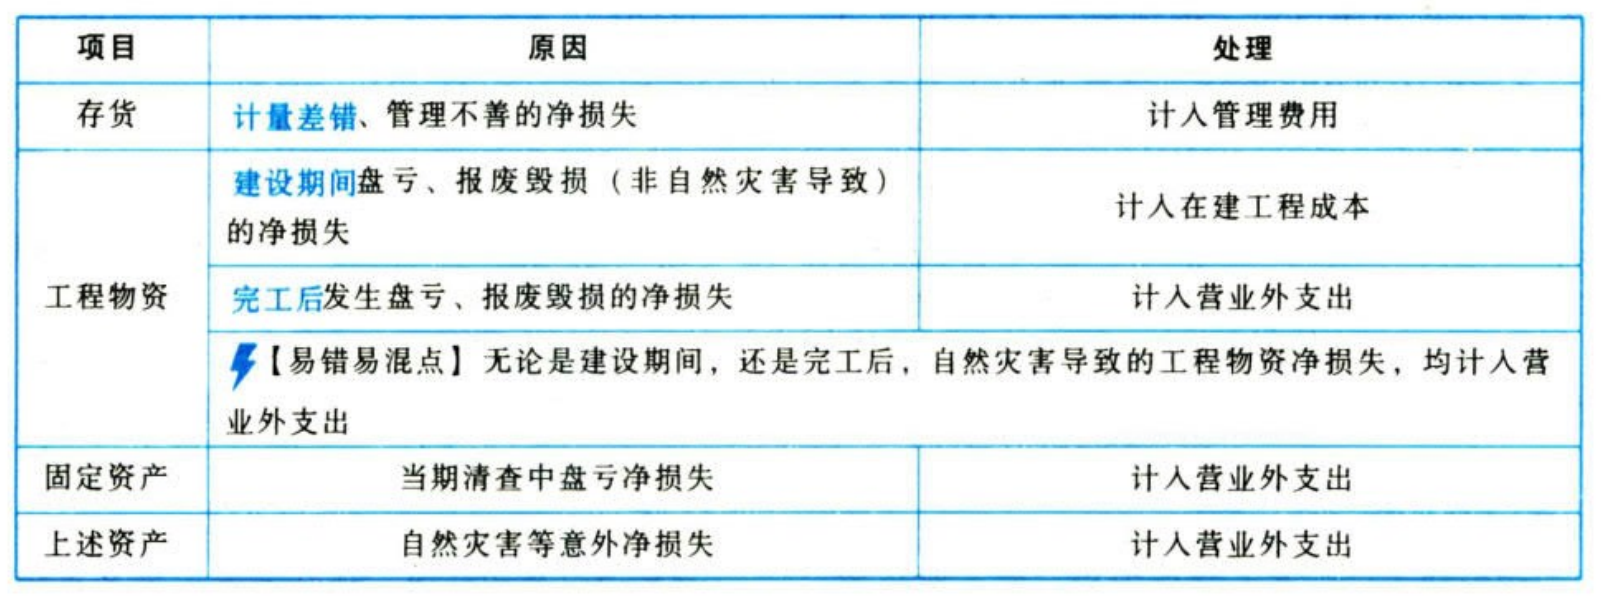
\includegraphics[width=1\linewidth]{pic/3.4.png}
		\caption{Caption}
		\label{fig:enter-label}
	\end{figure}
	
	\subsection{其他}
	由于固定资产的取得可能涉及到融资的方式取得,因此这里涉及到借款费用的问题
	
	
	
	\newpage
	\section{无形资产}
	
	无形资产:没有实物形态的可辨认非货币性资产。主要包括专利权、非专利技术、商标权、著作权、土地使用权、特许权等。
	
	\subsection{确认与初始计量}
	
	按照实际成本进行初始计量。不同的取得方式有着不同的计量方法。
	\begin{enumerate}
		\item 外购获得。达到预定可使用状态前的费用。具有融资性质的,以现值为基础进行摊销,采用实际利率法摊销(和固定资产类似)。
		
		\item 投资者投入。根据投资合同或协议确定成本。
		
		\item 非货币性资产交换、债务重组。根据另外两个细分准则进行确定。
		
		\item 政府补助。按公允价值进行计量。无公允价值按照名义金额。
		
		\item 土地使用权。可能作为不同的资产进行核算。固定资产、无形资产、投资性房地产、存货。
		
		土地使用权用于自行开发建造厂房等地上建筑物时,土地使用权与地上建筑物\textbf{分别}进行摊销和计提折旧。如果难以分配,则全部作为固定资产处理。
		
		\item 企业通过外购方式取得确认为无形资产的数据资源成本
		
		\item 企业合并中取得的无形资产成本。同控账面价值,非同控公允价值。
	\end{enumerate}
	
	\subsection{内部研究开发支出的确认和计量}
	内部研究需要区分\textbf{研究阶段与开发阶段}。
	
	研发支出可以可能\textbf{资本化计入无形资产},也可能\textbf{费用化计入管理费用}。
	
	一般来说开发阶段支出进行资本化、研究阶段以及无法资本化的开发阶段支出进行费用化。如果无法区分两个阶段则全部计入管理费用。(管理费用是会计科目、研发支出是报表项目)
	
	如果所发生的支出同时用于支持多项开发活动的,无法明确分配的不计入开发活动的成本。新产品专利支出属于无形资产成本。
	
	\paragraph{会计处理}
	企业发生的研发支出通过“研发支出”科目归集。下设子科目费用化支出与资本化支出。
	
	列报上,两个不同的子科目有着不同的列报方法。
	
	费用化支出科目余额期末转入管理费用-研究费用科目。研发项目形成无形资产后,管理用无形资产摊销计入管理费用-无形资产摊销。管理费用-研究费用与管理费用-无形资产摊销科目发生额在利润表研发费用项目列报
	
	资本化支出科目在达到预定可使用状态前在资产负债表开发支出列报。达到预定可使用状态后在无形资产列报。
	
	
	
	\subsection{后续计量}
	后续计量主要考虑摊销,分为寿命确定与不确定两种情况。预期寿命的确定还要收到和同行权利或其他法定权利规定的期限,不得高于这个值。如果有多个值,通常取最小的
	
	\textbf{寿命确定}的情况下需要进行摊销,方法与经济利益\textbf{预期消耗方式}有关(不是预期实现形式)。摊销一般计入当期损益,如果用于生产产品则会计入生产成本或制造费用。
	
	特殊情况下,收入可以作为无形资产摊销的基础,但是固定资产永远不行。
	
	一般情况下,无形资产残值都为0。
	
	\textbf{寿命不确定}的情况下需要在每期期末进行减值测试。
	
	这里需要注意无形资产摊销和固定资产折旧的\textbf{区别}。无形资产摊头不摊尾,固定资产摊尾不摊头。
	
	\subsection{处置}
	
	处置主要包括三种情况:出售、出租、报废。
	
	\subsubsection{出售}
	差额计入\textbf{资产处置损益}。值得注意,这里没有像固定资产一样有固定资产清理科目。
	
	\begin{Dr}
		银行存款
		
		无形资产减值准备
		
		累计摊销
	\end{Dr}
	\begin{Cr}
		无形资产
		
		应交税费-应交增值税(销项税额)
		
		资产处置损益
	\end{Cr}
	
	\subsubsection{出租}
	
	\textbf{确认收入}
	
	\begin{Dr}
		银行存款
	\end{Dr}
	\begin{Cr}
		其他业务收入
		
		应交税费-应交增值税(销项税额)
	\end{Cr}

	
	\textbf{相关费用计入成本}
	
	\begin{Dr}
		其他业务成本
	\end{Dr}
	\begin{Cr}
		累计摊销
		
		银行存款
	\end{Cr}
	
	
	\subsubsection{报废}
	
	不能带来价值,以账面价值\textbf{计入当期损益}
	
	\begin{Dr}
		营业外支出
		
		累计摊销
		
		无形资产减值准备
	\end{Dr}
	\begin{Cr}
		无形资产
	\end{Cr}

	
	\newpage
	\section{投资性房地产}
	
	本章主要关注后续计量模式的变更以及转换。
	
	投资性房地产:为\textbf{赚取租金}或\textbf{资本增值}而持有的房地产。
	
	主要包括\textbf{已出租的土地使用权}(计划但尚未的不算)、\textbf{持有并准备增值后转让的土地使用权}、\textbf{已出租的建筑物}(转租不算、管理层决定出租的也算,必须通过书面决议)。
	
	房地产可以有很多用途,如果无法区分则不确认为投资性房地产。
	
	\subsection{确认与初始计量}
	不同类型的房地产有着不同的确认时点
	\begin{enumerate}
		\item 已出租的土地使用权、建筑物。确认时点为租赁开始日
		
		\item 持有并准备增值后转让的土地使用权。确认时点为将自用土地使用权停止自用,准备增值后转让的日期
		
		\item 持有以被经营出租的控制建筑物或在建建筑物。确认时点为董事会或类似机构做出书面决议的日期。
	\end{enumerate}
	
	
	投资性房地产按成本计量。不同方式有着不同的计量方式。
	
	\begin{enumerate}
		\item 外购。外购直接用于投资和增值则计入无形资产,否则先计入固定资产和无形资产,后续开始租赁或用于增值则转换为投资性房地产。
		
		\item 自行建造。非正常损失计入当期损益,不计入建造成本。
	\end{enumerate}
	
	后续支出满足资本化的计入成本,在改扩建期间不进行折旧或摊销,分录上转入投资性房地产-在建(与固定资产的在建工程做区分)。不计入在建工程的原因是不利于财报的纵向分析(因为投资性房地产通常价值很高,这样会使得在建工程价值很高)
	
	后续费用化的支出计入当期损益(其他业务成本)。注意区分其他业务收入与营业外收入、主营业务收入。
	
	\subsection{后续计量}
	投资性房地产的后续计量可以分为\textbf{成本模式}或\textbf{公允价值模式}。两者的科目设置不同,会计处理也不同。
	
	成本模式类比固定资产和无形资产,损益类科目通常使用其他业务收入、其他业务成本。
	
	\subsubsection{成本模式}
	成本模式下科目为:投资性房地产、投资性房地产累计折旧(摊销)、投资性房地产减值准备。会计处理如下。
	
	\textit{计提折旧或摊销}
	
	\begin{Dr}
		其他业务成本
	\end{Dr}
	\begin{Cr}
		投资性房地产累计折旧(摊销)
	\end{Cr}
	
	\textit{计提减值准备}
	
	\begin{Dr}
		资产减值损失
	\end{Dr}
	\begin{Cr}
		投资性房地产减值准备
	\end{Cr}

	
	\textit{取得租金收入}
	
	\begin{Dr}
		银行存款
	\end{Dr}
	\begin{Cr}
		其他业务收入
		
		应交税费-应交增值税(销项税额)
	\end{Cr}
	
	值得注意的是,投资性房地产中土地使用权与建筑物的折旧和摊销和无形资产与固定资产的摊销方式相同。
	
	\subsubsection{公允价值模式}
	只有公允价值\textbf{可以可靠获得时}才可以使用公允价值模式。
	
	科目设置:投资性房地产-成本、投资性房地产-公允价值变动、公允价值变动损益。
	
	\textit{公允价值上升},下降做相反目录
	
	\begin{Dr}
		投资性房地产-公允价值变动
	\end{Dr}
	\begin{Cr}
		公允价值变动损益
	\end{Cr}

	\textit{取得租金收入}
	
	\begin{Dr}
		银行存款
	\end{Dr}
	\begin{Cr}
		其他业务收入
		
		应交税费-应交增值税
	\end{Cr}
	
	如果提供免租期,则应当将租金总额在不扣除免租期的整个租赁期间进行分配
	
	\subsubsection{模式改变}
	可以由成本模式转为公允价值模式,反之不行。此时作\textbf{为会计政策变更}处理,根据公允价值与账面价值的差额调整\textbf{期初留存收益}(不是其他损益类科目)。会计处理如下。
	
	\begin{Dr}
		投资性房地产(变更日公允价值)
		
		投资性房地产累计折旧(摊销)
		
		投资性房地产减值准备
	\end{Dr}
	\begin{Cr}
		投资性房地产(原价)
		
		盈余公积(或借方)
		
		利润分配-未分配利润(或借方)
	\end{Cr}

	首先冲减盈余公积,不够则冲减未分配利润
	
	\subsection{转换与处置}
	\subsubsection{转换}
	转换上可能存在“自用房地产与存货”和“投资性房地产”之间的转换。
	
	在成本模式下,两者之间按照账面价值进行互相转换。
	
	公允价值模式下,投资性房地产转非投资性,差额计入公允价值变动损益。\textbf{非投资性转投资性},借方差额计入公允价值变动损益,\textbf{贷方差额}计入其他综合收益。(首次确认公允价值调整,不直接计入损益,避免利润操纵)
	
	\subsubsection{处置}
	成本模式下和销售很类似,但是公允价值模式下需要额外考虑后续计量中的公允价值变动损益以及转换时产生的其他综合收益
	
	公允价值模式下公允价值变动不影响营业利润。其他综合收益对利润的影响需要调整
	
	
	\paragraph{成本模式下}
	
	\textbf{1.确认收入}
	
	\begin{Dr}
		银行存款
	\end{Dr}
	\begin{Cr}
		其他业务收入
		
		应交税费-应交增值税(销项税额)
	\end{Cr}

	
	\textbf{2.确认成本}
	
	\begin{Dr}
		其他业务成本
		
		投资性房地产累计折旧
		
		投资性房地产减值准备
	\end{Dr}
	\begin{Cr}
		投资性房地产
	\end{Cr}

	
	\paragraph{公允价值模式下}
	\textbf{1.确认收入}
	
	\begin{Dr}
		银行存款
	\end{Dr}
	\begin{Cr}
		其他业务收入
		
		应交税费-应交增值税
	\end{Cr}
	
	
	\textbf{2.确认成本}
	
	\begin{Dr}
		其他业务成本
	\end{Dr}
	\begin{Cr}
		投资性房地产-成本
		
		投资性房地产-公允价值变动
	\end{Cr}
	
	
	\textit{转出公允价值变动损益,不影响营业利润}
	
	\begin{Dr}
		公允价值变动损益
	\end{Dr}
	\begin{Cr}
		其他业务成本
	\end{Cr}
	
	若涉及其他综合收益(公允价值模式下其他资产转为投资性房地产)做下列分录,使得\textbf{营业利润增加}
	
	\begin{Dr}
		其他综合收益
	\end{Dr}
	\begin{Cr}
		其他业务成本
	\end{Cr}

	\subsection{其他}
	自然灾害损失如何计量
	
	各种类型的修理费用如何计量
	
	\newpage
	\section{长期股权投资与合营安排}
	\subsection{基本概念}
	\paragraph{股权投资}
	首先对外投资来说可以分为股权投资和其他投资。而股权投资又包括了长期股权投资以及《金融工具确认与计量》所规定的股权投资。
	
	只有\textbf{控制的子公司}、\textbf{共同控制的合营企业}以及\textbf{重大影响的联营企业}才能使用长期股权投资准则进行核算。
	
	有关控制的定义,则和持股比例有关。持股100-50可以称作控制,持股50-20可以称作共同控制或重大影响,持股20以下则属于三无。
	
	\paragraph{联营企业投资}
	对联营企业投资,是指投资方能够对被投资单位施加重大影响的股权投资。重大影响是指投资方对被投资单位的财务和生产经营决策有参与决策的权力,但并不能控制或与其他方一起共同控制这些政策的制定。
	
	通常可以通过以下几种方式来判断
	\begin{enumerate}
		\item 在被投资单位的董事会中派有代表
		
		\item 参与被投资单位财务和经营决策制定过程
		
		\item 与被投资单位之间发生重要交易
		
		\item 向被投资单位派出管理人员
		
		\item 向被投资单位提供关键技术材料
	\end{enumerate}
	
	重大影响的判断关键是分析投资方是否有实质性的参与权而不是决定权。
	
	\paragraph{合营企业投资}
	对合营企业投资,是指投资方与其他合营方一同对被投资单位实施共同控制且对被投资单位净资产享有权利的权益性投资。
	
	共同控制包含合营企业以及共同经营两种情况。本章最后一节会详细分析共同控制
	
	\paragraph{对子公司投资}
	对子公司投资,是指投资方持有的能够对被投资单位施加控制的权益性投资。控制的界定及判断请见二十七章。
	
	\subsection{初始计量}
	初始计量最主要的是要确定\textbf{初始投资成本}。虽然都叫初始投资成本,但是不同的长投初始投资成本计量方式不同。
	
	对联营企业、合营企业的投资,初始投资成本用\textbf{支付价款的公允价值+初始直接费用}计量
	
	对子公司投资(企业合并)需要区分同一控制下和非同一控制下。
	\begin{enumerate}
		\item 同一控制下,取得被合并方所有者权益在\textbf{最终控制方合并财务报表中的账面价值份额+最终控制方收购被合并方时形成的商誉}。
		
		\item 非同一控制下,通常情况下为\textbf{公允价值}。
	\end{enumerate}
	
	\textbf{同控}是指参与合并的企业在合并前后均受同一方或相同的多方最终控制且该控制并非暂时性的
	
	\textbf{非同控}是指参与合并各方在合并前后不受同一方或相同的多方最终控制的合并交易,即同控下企业合并以外的其他企业合并。
	
	\subsubsection{长期股权投资的确认}
	长期股权投资的\textbf{确认的时点}:是指投资方能够在自身账簿和报表中确认对被投资单位股权投资的时点。购买方(或合并方)应于购买日(或合并日)确认对子公司的长期股权投资。
	
	对于合并日(或购买日)的判断,满足以下有关条件的,通常可认为实现了控制权的转移
	\begin{enumerate}
		\item 企业合并合同或协议已获股东大会通过;
		
		\item 企业合并事项需要经过国家有关主管部门审批的,已获得批准;
			
		\item 参与合并各方已办理了必要的财产权转移手续;
		
		\item 合并方或购买方已支付了合并价款的大部分(一般应超过50\%),并且有能力、有计划支付剩余款项;
		
		\item 合并方或购买方实际上已经控制了被合并方或被购买方的财务和经营政策,并享有相应的利益、承担相应的风险。
	\end{enumerate}
	
	
	对于认缴制下尚未出资的股权投资,投资方在未实际出资前是否应确认与所认缴出资相关的股权投资,应结合法律法规规定与具体合同协议确定(\textbf{有合同,同时确认资产与负债;无合同不确认}):
	\begin{enumerate}
		\item 若合同明确约定认缴出资的时间和金额,且投资方按认缴比例有相应的股东权益,则投资方应确认一项金融负债(其他应付款)及相应的资产(长期股权投资);
		
		\item 若合同没有明确约定,则属于一项未来的出资承诺,不确认金融负债及相应的资产。
	\end{enumerate}

	\subsubsection{对联营企业、合营企业投资的初始计量}
	取得的方式不同,初始投资成本计量不同。但是大致思路是以\textbf{付出对价的公允价值进行计量}。需要注意的是对于其中费用的计量。
	\begin{enumerate}
		\item 以支付现金取得。实际支付的购买价款(包括与取得长期股权投资直接相关的费用、税金及其他必要支出)
		
		\item 以发行权益性证券取得。权益性证券的公允价值+直接相关费用
		
		\item 以债务重组、非货币性资产交换等方式取得。按债务重组、非货币性资产交换等相关准则规定处理
	\end{enumerate}
	
	\subsubsection{对子公司的初始计量}
	\paragraph{同一控制下控股合并形成的对子公司长期股权投资}
	同控下的处理基本原则是\textbf{权益结合法},和购买法不同。因为当完成合并后,从母公司的角度来看并未流出资产、也未承担子公司的债务。因此有观点认为在合并报表中被合并方的资产和负债可以按\textbf{账面价值}入账。
	
	因此同控下企业合并不产生新的资产、负债或商誉,确认的商誉应作为资产确认。
	
	不同的取得方式下有着不同的会计分录,具体情形如下
	
	\textit{合并方以支付现金、转让非现金资产或承担债务方式作为合并对价}
	
	\begin{Dr}
		长期股权投资(取得被合并方所有者权益在最终控制方合并财务报表中的账面价值份额+最终控制方收购被合并方时形成的商誉)
	\end{Dr}
	\begin{Cr}
		负债(承担债务账面价值)
		
		资产(投出资产账面价值)
		
		资本公积-资本溢价/股本溢价(差额)
	\end{Cr}
	
	\begin{Dr}
		管理费用(审计、法律服务、评估咨询等中介费用以及其他相关管理费用)
	\end{Dr}
	\begin{Cr}
		银行存款
	\end{Cr}
	
	\textit{合并方以发行权益性证券作为合并对价}。发行证券冲减资本公积
	
	\begin{Dr}
		长期股权投资(取得被合并方所有者权益在最终控制方合并财务报表中的账面价值份额+最终控制方收购被合并方时形成的商誉)
	\end{Dr}
	\begin{Cr}
		股本
		
		资本公积-股本溢价
	\end{Cr}
	
	\begin{Dr}
		资本公积-股本溢价等(权益性证券发行费用)
	\end{Dr}
	\begin{Cr}
		银行存款
	\end{Cr}
	
	同控下的企业合并,无论是一次交易还是多次交易,初始投资成本都类似。但是多次交易时,可能存在调整的情况
	
	初始投资成本与达到合并前的长期股权投资账面价值加上合并日进一步取得股份新支付对价的账面价值之和的差额,调整资本公积(股本溢价或资本溢价),资本公积不足冲减的,冲减留存收益。
	
	
	
	\paragraph{非同一控制下控股合并形成的对子公司长期股权投资}
	
	基本处理原则是购买法
	
	\textit{一次交易形成的}
	将企业合并成本作为长期股权投资的初始投资成本。企业合并成本包括付出所有东西在购买日的公允价值。公允价值和账面价值的差额计入当期损益或留存收益
	
	相关费用和同控处理情况类似。
	
	具体来说,根据付出的资产不同,账面价值和公允价值之间差额的处理也不同。核心思想是把资产卖了,然后再买长投
	\begin{enumerate}
		\item 固定资产/无形资产。计入资产处置损益
		
		\item 存货。确认收入结转成本,同时结转存货跌价准备
		
		\item 其他债权投资。公允价值与账面价值的差额计入投资收益,持有期间因公允价值变动形成的其他综合收益一并转入投资收益。
		
		\item 投资性房地产。确认其他业务收入与成本。同时结转确认期间的公允价值变动损益与其他综合收益
	\end{enumerate}
	
	\textit{多次交易形成的}
	如果原投资为权益法核算的长期股权投资。购买日长期股权投资初始投资成本=购买日原投资账面价值+新增投资公允价值
	
	原投资为以公允价值计量且其变动计入当期损益的金融资产。初始投资成本=购买日原投资公允价值+新增投资公允价值
	
	原投资为以公允价值计量且其变动计入其他综合收益的非交易性权益工具投资。初始投资成本=购买日原投资公允价值+新增投资公允价值
	
	
	\paragraph{投资成本中包含的已宣告但尚未发放的现金股利或利润的处理}
	不构成长期股权投资成本,单独作为应收项目处理,计入应收股利科目。
	
	有关长投初始计量和相关费用的计量总结在章节最后表\ref{longterm investment initial,longterm investment initial fee}
	
	
	\subsection{后续计量}
	
	\subsubsection{成本法}
	投资方能够对被投资单位实施\textbf{控制}的长期股权投资应当采用成本法核算。
	
	成本法是指投资按成本计价的方法。长期股权投资科目反映取得时的成本。长投的入账减值就通过初始投资成本来计量,不需要调整(和权益法对应)。在核算过程中主要注意的事项有发放现金股利和计提减值准备。
	
	\textit{被投资单位宣告发放现金股利时}
	
	\begin{Dr}
		应收股利
	\end{Dr}
	\begin{Cr}
		投资收益
	\end{Cr}
	
	\textit{计提减值准备时(长投减值准备不可转回)}
	
	\begin{Dr}
		资产减值损失
	\end{Dr}
	\begin{Cr}
		长期股权投资减值准备
	\end{Cr}
	
	处置长期股权投资,应将长期股权投资账面价值与实际取得价款的差额计入当期损益(投资收益)
	
	\subsubsection{权益法}
	成本法不关注被投资单位所有者权益的变动。权益法关注。权益法更复杂的原因是被投资单位的许多经营活动会影响利润,从而影响所有者权益,因此权益法需要考虑更多的因素。
	
	
	权益法的使用范围主要包括共同控制的合营企业、重大影响的联营企业。
	
	权益法的会计科目有四个
	\begin{enumerate}
		\item 投资成本。投资时点
		
		\item 损益调整。持有期间被投资单位净损益变动及利润分配
		
		\item 其他综合收益。持有期间被投资单位其他综合收益变动
		
		\item 其他权益变动。持有期间被投资单位其他权益变动
	\end{enumerate}
	投资成本核算投资时点,后三个明细科目核算投资后。
	
	
	
	
	\paragraph{初始投资成本的调整}
	长期股权投资的初始投资成本\textbf{大于}投资时应享有的被投资单位可辨认净资产公允价值份额,则\textbf{不调整}长期股权投资的初始投资成本。(实际上是商誉,不在个别报表体现,在合并报表体现)
	
	长期股权投资的初始投资成本\textbf{小于}投资时应享有的被投资单位可辨认净资产公允价值份额,其差额体现主体经济利益流入,应作为收益计入营业外收入(简单来说就是投资赚钱了记营业外收入),分录为
	
	\begin{Dr}
		长期股权投资-投资成本
	\end{Dr}
	\begin{Cr}
		营业外收入
	\end{Cr}
	
	
	
	\paragraph{投资损益的确认}
	投资企业取得长期股权投资后,应当按照应享有的或应分担的被投资单位实现的净损益的份额,确认投资损益并调整长期股权投资的账面价值。
	
	\textit{被投资单位实现净利润}
	
	\begin{Dr}
		长期股权投资-损益调整
	\end{Dr}
	\begin{Cr}
		投资收益
	\end{Cr}
	
	\textit{被投资单位实现净亏损}
	
	\begin{Dr}
		投资收益
	\end{Dr}
	\begin{Cr}
		长期股权投资-损益调整
	\end{Cr}
	
	此外还有一些需要注意的事项
	\begin{enumerate}
		\item 被投资单位采用的会计政策与会计期间与投资方不一致的,应按投资方的口径进行调整
		
		\item 投资方在确认应享有被投资单位净损益的份额时,应当以取得投资时被投资单位\textbf{可辨认净资产的公允价值为基础},对被投资单位的\textbf{净损益进行调整后确认}。
	\end{enumerate}
	
	此外还有一个非常重要且复杂的影响损益的因素,\textbf{内部交易}。首先我们要区分内部交易是否构成业务
	\begin{enumerate}
		\item 构成业务。(简言之就是不需要抵销,而不构成业务则可能需要在合并报表层面抵销)
		\begin{enumerate}
			\item \textbf{被投资方向投资方出售业务的},投资采用权益法进行核算时,对于出售该业务而产生的损益,\textbf{不予抵销}。
			
			\item \textbf{投资方向被投资方投出业务},投资方因此取得长期股权投资但未取得控制的,以投出业务的公允价值作为新增长期股权投资的初始成本,与账面价值之间的差额计入当期损益(回忆初始投资的情形,和多次交易形成类似)
			
			\item \textbf{投资方向被投资方出售业务},取得对价与业务的账面价值之间的差额,全额计入当期损益。
		\end{enumerate}
		
		\item 不构成业务。则区分逆流交易与顺流交易进行处理
	\end{enumerate}	
	
	如果不构成业务,则对于\textbf{投资方或纳入投资方}合并财务报表范围的子公司与\textbf{其联营企业及合营企业之间}发生的未实现内部交易损益应予以抵消。(但是存在区别,母子公司是全额抵销,合营联营是按比例取消)
	
	首先区分逆流交易和顺流交易。逆流交易就是\textbf{被投资企业出售资产给投资企业},顺流交易则时\textbf{投资企业投出或出售资产给被投资企业}。这两种交易重点都是需要在合并报表中进行抵消操作。
	
	对于\textbf{逆流交易}来说,投资企业应该抵销未实现内部交易的损益的影响。损益影响了两方面的问题
	\begin{enumerate}
		\item 被投资方的净收益需要进行调整,根据调整后的净收益来计算长投的损益调整
		
		\item 投资方的合并财务报表中(如果投资方还控制其他子公司,则需要编制合并财务报表),抵销有关资产账面价值中包含的未实现内部交易损益,并调整对应的长投。调整分录如下
	\end{enumerate}
	
	\begin{Dr}
		长期股权投资
	\end{Dr}
	\begin{Cr}
		xx资产(结存资产中的未实现内部销售利润*投资方持股比例)
	\end{Cr}
	
	调整的主要原因在于,因逆流交易而产生的未实现内部交易损益在为对外部独立第三方出售或被耗用之前,体现在投资企业持有资产的账面价值之中。因此需要调整。(就是合并报表中的抵销分录)
	
	对于\textbf{顺流交易}来说,投资企业也应当抵销该未实现内部交易损益的影响。损益主要影响了两个方面的问题(第一个和逆流相同,第二个和逆流不同)
	\begin{enumerate}
		\item 被投资方的净收益需要进行调整,根据调整后的净收益来计算长投的损益调整
		
		\item 投资方的合并财务报表中(如果投资方还控制其他子公司,则需要编制合并财务报表)调整收入,只确认归属于被投资方其他投资者部分的损益,归属于本企业的部分不予确认(即进行抵销)。调整分录如下
	\end{enumerate}
	
	\begin{Dr}
		营业收入(内部销售收入 $\times$ 内部结存比例 $\times$ 投资方持股比例)
	\end{Dr}
	\begin{Cr}
		营业成本(内部销售成本 $\times$ 内部结存比例 $\times$ 投资方持股比例)
		
		投资收益
	\end{Cr}
	
	后续期间商品实现对外出售时,应对前期顺流交易未实现损益确认有关收入并结转成本,或
	
	\begin{Dr}
		资产处置收益(内部交易产生的资产处置损益中未实现部分 $\times$ 投资方持股比例)
	\end{Dr}
	\begin{Cr}
		投资收益 
	\end{Cr}
	
	
	总结来看,所有这些内部交易都要考虑\textbf{两部分问题,即长投在个别报表的分录以及在合并报表中的抵消分录}。
	\begin{enumerate}
		\item 子公司利润变化对于母公司个别报表中长投损益调整科目的影响
		
		\item 子公司经营活动在母公司合并报表中是否需要做抵销分录,抵销分录根据顺流和逆流交易情况做不同分录。
	\end{enumerate}
	
	有关损益的总结在本章最后表\ref{profits and losses to longterm investment}
	
	
	
	
	\paragraph{被投资单位宣告分配现金股利或利润的处理}股票股利不做处理,但应于除权日注明所增加的股数,普通现金股利分录如下
	
	\begin{Dr}
		应收股利
	\end{Dr}
	\begin{Cr}
		长期股权投资-损益调整
	\end{Cr}
	
	
	
	\paragraph{其他综合收益的处理}
	被投资单位其他综合收益发生变动的,投资方应当按照归属于本企业的部分,相应调整长期股权投资的账面价值,同时增加或减少其他综合收益
	
	\begin{Dr}
		长期股权投资-其他综合收益
	\end{Dr}
	\begin{Cr}
		其他综合收益
	\end{Cr}
	
	\paragraph{被投资单位所有者权益其他变动的处理}
	被投资单位除净损益、其他综合收益以及利润分配以外的所有者权益的其他变动,应按所持股权比例计算应享有的份额,调整长期股权投资的账面价值,同时计入\textbf{资本公积-其他资本公积},并在备查簿中予以登记
	
	\begin{Dr}
		长期股权投资-其他权益变动
	\end{Dr}
	\begin{Cr}
		资本公积-其他资本公积
	\end{Cr}
	
	投资方在后续处置股权投资但对剩余股权仍采用权益法核算时,应按\textbf{处置比例将这部分资本公积转入当期投资收益}。对剩余股权终止权益法核算时,将这部分资本公积全部转入当期投资收益。
	
	\begin{Dr}
		资本公积-其他资本公积
	\end{Dr}
	\begin{Cr}
		投资收益
	\end{Cr}
	
	所有者权益的其他变动主要包括
	\begin{enumerate}
		\item 被投资单位接受其他股东的资本性投入
		
		\item 被投资单位发行可分离可交易的可转换公司债券中包含的权益成分
		
		\item 以权益结算的股份支付
		
		\item 其他股东对被投资单位增资导致投资方持股比例变化(稀释股权)等
	\end{enumerate}
	
	\paragraph{超额亏损}
	发生亏损时,以0为限。但是存在特殊情况。如果不扣抵扣,则按以下顺序抵扣:长期股权投资、长期应收款、预计负债。如果后续盈利则反向
	
	\paragraph{因被动稀释导致持股比例下降时,内含商誉的结转} 这里是将所有者权益其他变动的第四种情况展开来进行分析。
	
	这一情形下,如果因稀释而产生损失,则应该作为减值迹象,进行减值测试。
	
	此外,还要考虑稀释后的账面价值,根据商誉以及稀释后享有净资产公允价值的份额(从购买日开始计算至稀释日)计算长投账面价值
	
	\paragraph{减值}
	同其他资产、略过。
	
	\subsection{核算方法的转换与处置}
	总体来说,需要考虑转换情形是上升还是下降了。核算方法从持股高低可以分为成本法、权益法、公允价值。所以总共有六种情况,上升有三种情况,下降有三种情况。
	
	值得注意的是,长期股权投资的核算方法只有成本法和权益法,但是金融工具的核算方法有公允价值计量。这里的转换是考虑到了金融工具转化为长期股权投资的情况
	
	无论上升还是下降的情况,总体原则都是基于\textbf{公允价值}去进行调整。上升的情况下,将原投资调整到公允价值;下降的情况下,将剩余投资调整到公允价值。
	
	但是成本法和权益法之间互相转换的情况下,在个别报表调整到公允价值会违背历史成本计量属性,因此在合并财务报表中将原投资调整到公允价值。
	
	不同情形的会计处理如下
	\begin{enumerate}
		\item 公允价值计量转为权益法,个别财务报表中原投资调整到公允价值。
		
		\item 权益法转为成本法,个别财务报表保持原投资账面价值,合并财务报表原投资调整到公允价值
		
		\item 公允价值计量转为成本法(非同控),个别财务报表中原投资调整到公允价值。
		
		\item 成本法转为权益法,剩余投资调整追溯调整未权益法核算的账面价值,合并财务报表剩余投资调整到公允价值。
		
		\item 权益法转为公允价值计量,个别财务报表中原投资调整到公允价值。
		
		\item 成本法转为公允价值计量,个别财务报表中原投资调整到公允价值。
	\end{enumerate}
	
	
	\subsubsection{成本法转权益法}
	这种情况下需要分别考虑个别报表和合并报表的情况。
	
	首先考虑\textbf{个别报表}的情况,个别报表主要做两个事情,一个是处置时分录,另一个是基于权益法追溯调整账面价值。处置部分分录如下
	
	\begin{Dr}
		银行存款
	\end{Dr}
	\begin{Cr}
		长期股权投资
		
		投资收益
	\end{Cr}
	
	剩余部分\textbf{追溯调整}。首先追溯调整投资时点的商誉,如果成本大于份额,则不调整长投账面价值,如果小于份额,则调整长投成本的同时调整留存收益,如果在同一个会计年度,则调整当期损益(营业外收入)
	
	此外投资后的时点也需要追溯调整,如果是期初之前的损益则调整留存收益,如果是期初之后的则调整投资收益(逻辑和商誉的调整类似)
	
	\begin{Dr}
		长期股权投资
	\end{Dr}
	\begin{Cr}
		留存收益(原投资时至处置投资当期期初被投资单位实现的净损益(扣除已发放的现金股利与利润分配)*剩余持股比例)
		
		投资收益(处置投资当期期初至处置投资日被投资单位实现的净损益(扣除已发放的现金股利与利润分配)*剩余持股比例)
		
		其他综合收益(被投资单位其他综合收益变动*剩余持股比例)
		
		资本公积-其他资本公积(其他原因导致的被投资单位所有者权益的变动)
	\end{Cr}
	
	在\textbf{合并报表}中,因为处置部分股权投资而丧失控制的,应当按照\textbf{丧失控制权日的公允价值}进行重新计量。处置股权取得的对价和剩余股权公允价值之和,减去按原持股比例计算应享有原子公司子购买日开始持续计算的净资产份额与商誉之和的差额,计入丧失控制权当期的投资收益。
	
	此外,与原有子公司股权投资相关的其他综合收益、其他所有者权益变动应当在丧失控制权时一并转入投资收益。
	
	简单来说,可以视为把所有股权卖了,然后再以公允价值购买股权。
	
	丧失控制权日合并财务报表中的投资收益=处置股权取得的对价与剩余股权公允价值之和-按原持股比例计算应享有原有子公司自购买日开始持续计算的净资产份额-商誉+与原有子公司股权投资相关的其他综合收益、其他权益变动
	
	在合并报表中主要做三个调整分录
	\begin{enumerate}
		\item 将剩余股权投资有个别报表中按权益法追溯调整后的账面价值调整到丧失控制权日的公允价值,调整分录未借记长期股权投资、贷记投资收益
		
		\item 对个别报表中确认的投资收益的归属期间进行调整,其调整分录为借记投资收益,贷记盈余公积、未分配利润、其他综合收益、资本公积
		
		\item 调整原有投资相关的其他综合收益、其他权益变动计入投资收益或留存收益。根据是否可以转损益以及是否可以转留存收益来决定
	\end{enumerate}
	
	\subsubsection{公允价值或权益法转成本法(非同控)}
	如果原投资是权益法,则追加投资日的长投投资成本=转换日原投资账面价值+新增投资成本
	
	如果原投资是公允价值,则追加投资日的长投投资成本=转换日原投资公允价值+新增投资成本
	
	合并报表的处理参见合并报表章节中,企业因追加投资等原因能够对非同一控制下的被投资方实施控制的相关处理。
	
	\subsubsection{公允价值计量转为权益法}
	
	追加投资日长期股权投资初始投资成本=转换日原投资公允价值+新增投资成本
	
	原持有的股权投资分类为其他权益工具投资的,将其他权益工具投资账面价值调整到公允价值,计入其他综合收益的累计公允价值变动应当转入留存收益
	
	在此基础上,和权益法类似,需要比较初始投资成本呢与可辨认净资产公允价值份额之间的差别,大于不调整,小于计入当期营业外收入。
	
	\subsubsection{权益法转为公允价值计量}
	\textit{处置部分}
	
	\begin{Dr}
		银行存款
	\end{Dr}
	\begin{Cr}
		长期股权投资(处置部分的投资的账面价值)
		
		投资收益(可借可贷)
	\end{Cr}
	
	\textit{原权益法核算确认的全部其他综合收益转入当期损益或留存收益}
	
	\begin{Dr}
		其他综合收益
	\end{Dr}
	\begin{Cr}
		投资收益(可转损益部分)
		
		盈余公积(不可转损益部分)
		
		利润分配-未分配利润
	\end{Cr}
	
	\textit{原权益法核算确认的全部资本公积转入当期损益}
	
	\begin{Dr}
		资本公积-其他资本公积
	\end{Dr}
	\begin{Cr}
		投资收益
	\end{Cr}
	
	\textit{剩余股转为交易性金融资产或其他权益工具}
	
	\begin{Dr}
		交易性金融资产/其他权益工具(公允价值)
	\end{Dr}
	\begin{Cr}
		长期股权投资(账面价值)
		
		投资收益(差额)
	\end{Cr}
	
	要结转其他综合收益以及资本公积是因为,这里的操作也视为把原有股权全部卖出然后再以公允价值买入。
	
	\subsubsection{成本法转为公允价值计量}
	\textit{确认有关股权投资的处置损益}
	
	\begin{Dr}
		银行存款
	\end{Dr}
	\begin{Cr}
		长期股权投资
		
		投资收益
	\end{Cr}
	
	\textit{剩余股权投资转为交易性金融资产或其他权益性工具}
	
	\begin{Dr}
		交易性金融资产/其他权益工具投资
	\end{Dr}
	\begin{Cr}
		长期股权投资
		
		投资收益
	\end{Cr}
	
	
	
	\subsubsection{长期股权投资处置}
	出售所得价款与长投账面价值之间的差额计入投资收益。
	
	此外,由于权益法核算中会涉及到其他综合收益以及资本公积等其他项目,所以处置时还需要做额外的会计分录。
	
	原权益法核算的相关其他综合收益应当采用与被投资单位直接处置相关资产或负债相同的基础进行会计处理。
	
	权益法核算投资处置后还是权益法核算,其他综合收益与资本公积-其他资本公积按处置比例结转。如果转为公允价值计量,则全部结转。
	
	
	
	\subsection{合营安排}
	合营安排:是指一项由两个或两个以上的参与方共同控制的安排。
	
	合营安排同时具有以下特征(2 个特征)
	1.	各参与方受到该安排的约束
	2.	两个或两个以上的参与方对该安排实施共同控制
	
	共同控制:是指按照相关约定对某项安排所共同的控制,并且该安排的相关活动必须经过分享控制权的参与方一致同意后才能决策。共同控制的判断中,首先判断是否由所有参与方或参与方组合集体控制该安排;再判断该安排相关活动的决策是否必须经过这些参与方一致同意
	
	①如果所有参与方或一组参与方必须一致行动才能决定某项安排的相关活动,则称所有参与方或一组参与方集体控制该安排。(不能是单独一方)
	②在判断集体控制时,需要注意以下3点:
	a.集体控制不是单独一方控制。
	b.尽管所有参与方联合起来一定能够控制该安排,但集体控制下,集体控制该安排的组合指的是那些既能联合起来控制该安排,又使得参与方数量最少的一个或几个参与方组合。
	c.能够集体控制一项安排的参与方组合很可能不止一个。
	
	如果存在两个或以上的参与方组合能够集体控制某安排,则不构成共同控制。
	
	只要两个或两个以上的参与方对该安排实施共同控制,一项安排就可以被认定为合营安排,并不要求所有参与方都对该安排享有共同控制。
	
	对合营安排享有共同控制的参与方(分享控制权的参与方)被称为“合营方”;对合营安排不享有共同控制的参与方被称为“非合营方”
	
	合营安排可以分为共同经营与合营企业。共同经营:是指合营方享有该安排相关资产且承担该安排相关负债的合营安排。营企业:是指合营方仅对该安排的净资产享有权利的合营安排
	
	单独主体是指具有单独可辨认的财务架构的主体,包括单独的法人主体和不具备法人资格但法律所认可的主体。单独主体并不一定要具备法人资格,但必须具有法律所认可的单独可辨认的财务架构,确认某主体是否属于单独主体必须靠考虑使用的法律法规。
	
	\begin{figure}
		\centering
		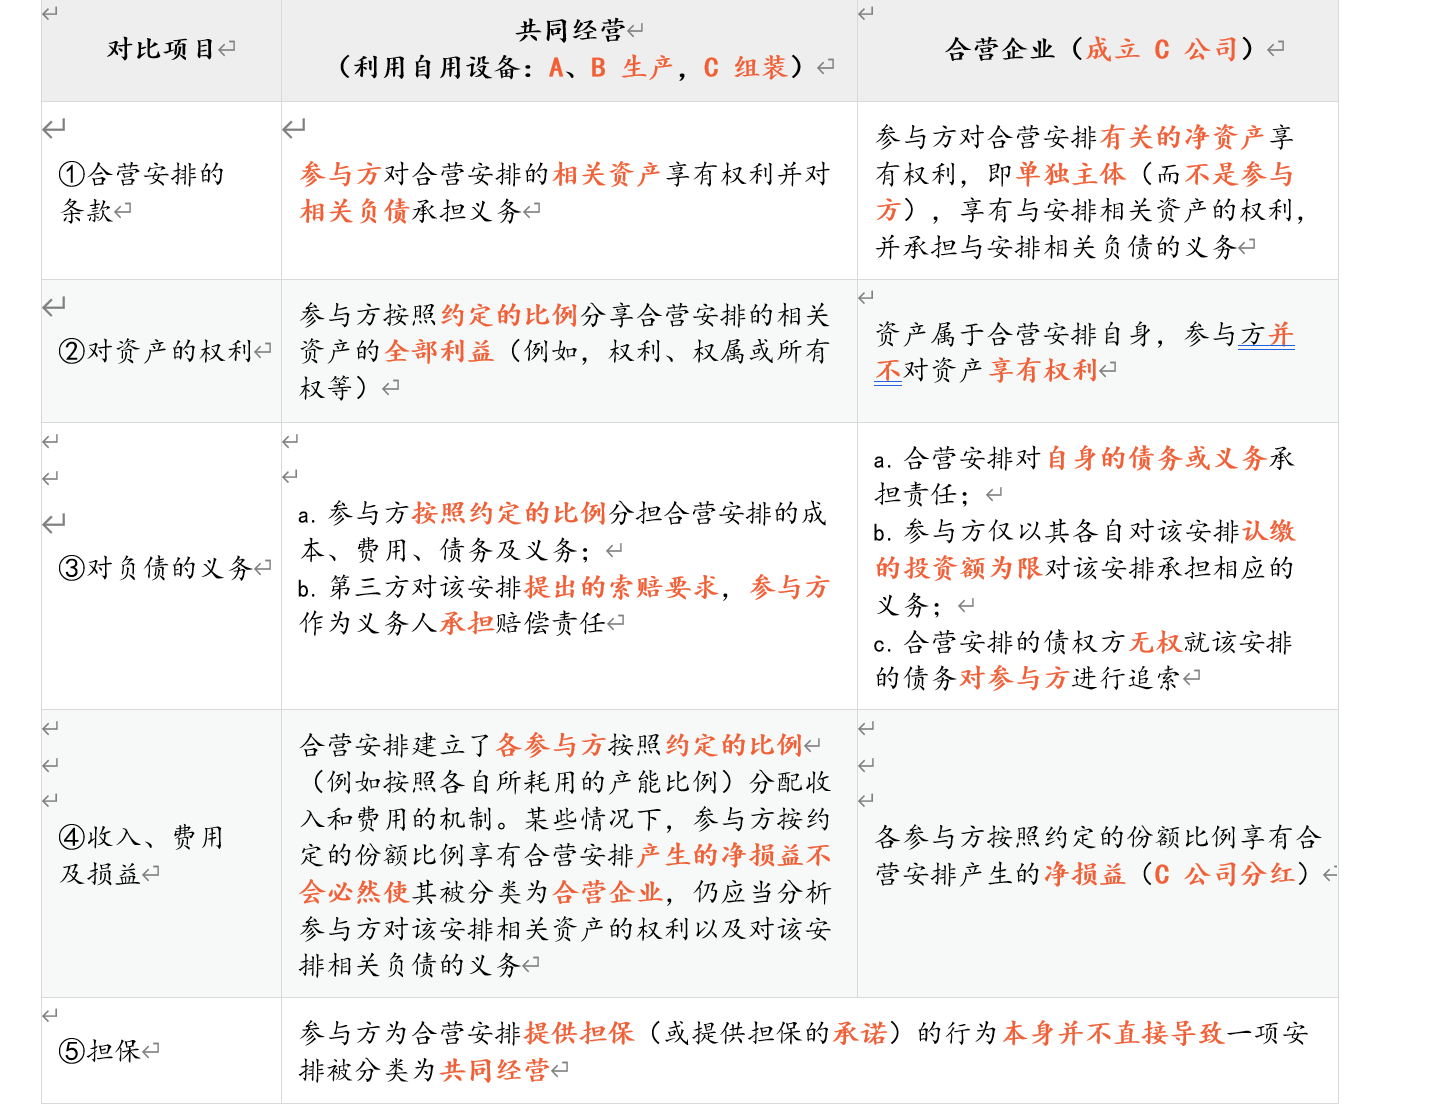
\includegraphics[width=0.7\linewidth]{pic/合营安排}
		\caption{}
		\label{fig:}
	\end{figure}
	
	企业对合营安排是否拥有共同控制权,以及评估该合营安排是共同经营还是合营企业,这需要企业予以判断并持续评估。在进行判断时,企业需要对所有的相关事实和情况加以考虑。
	
	\subsubsection{合营方的会计处理原则}
	1.一般会计处理原则(A生产甲配件、B生产乙配件,C组装后,进行销售)除合营方对持有合营企业投资应当采用权益法核算以外,其他合营安排中的合营方应当确认自身所承担的以及按比例享有或承担的合营安排中按照合同、协议等的规定归属于本企业的资产、负债、收入及费用。该处理方法一定程度上类似于比例合并,但与比例合并又存在差异。具体如下:合营方应当确认其与共同经营中利益份额相关的下列项目,并按照相关企业会计准则的规定进行会计处理:
	①确认单独所持有的资产,以及按其份额确认共同持有的资产
	②确认单独所承担的负债,以及按其份额确认共同承担的负债;
	③确认出售其享有的共同经营产出份额所产生的收入;
	④按其份额确认共同经营因出售产出所产生的收入;
	⑤确认单独所发生的费用,以及按其份额确认共同经营发生的费用。
	
	2.合营方向共同经营投出或者出售不构成业务的资产的会计处理(类似顺流交易)
	合营方向共同经营投出或出售资产等(该资产构成业务的除外),在共同经营将相关资产出售给第三<方或相关资产消耗之前(即未实现内部利润仍包括在共同经营持有的资产账面价值中时),应当仅确认归属于共同经营其他参与方的利得或损失。
	
	交易表明投出或出售的资产发生符合《企业会计准则第8号--资产减值》等规定的资产减值损失的,合营方应当全额确认该损失。
	
	3.合营方自共同经营购买不构成业务的资产的会计处理(类似逆流交易
	合营方自共同经营购买资产等(该资产构成业务的除外),在将该资产等出售给第三方之前(即未实现内部利润仍包括在合营方持有的资产账面价值中时),不应当确认因该交易产生的损益中该合营方应享有的部分。即,此时应当仅确认因该交易产生的损益中归属于共同经营其他参与方的部分。
	
	4.合营方取得构成业务的共同经营的利益份额的会计处理(换入)
	合营方取得共同经营中的利益份额、且该共同经营构成业务时,应当按照企业合并准则等相关准则进行相应的会计处理。(可以理解为购买企业,确认商誉)(
	合营方增加其持有的一项构成业务的共同经营的利益份额时,如果合营方对该共同经营仍然是共同控制,则合营方之前持有的共同经营的利益份额,不应按照新增投资日的公允价值重新计量。(A、B共同设立安排C,甲将A在C的利益份额全部购买,则不应该对C重新计量)
	
	\subsubsection{对非合营方的会计处理原则}
	对共同经营不享有共同控制的参与方(非合营方),如果享有该共同经营相关资产且承担该共同经营相关负债的,比照合营方进行会计处理。
	否则,应当按照相关企业会计准则的规定对其利益份额进行会计处理。
	例如:1.如果该参与方对于合营安排的净资产享有权利并且具有重大影响,则按照长期股权投资准则等相关规定进行会计处理;。
	2.如果该参与方对于合营安排的净资产享有权利并且无重大影响,则按照金融工具确认和计量准则等相关规定进行会计处理;
	3.向共同经营投出构成业务的资产的,以及取得共同经营的利益份额的,则按照合并财务报表及企业合并等相关准则进行会计处理。
	
	\subsection{其他}
	关于交易中其他交易费用的处理。为取得一项资产发生的直接相关费用一般应计入取得资产成本(参考固定资产、无形资产),但是对子公司投资发生的直接相关费用计入管理费用,具体原因参见26章企业合并。
	
	区分风投机构对于长投的处理方法。
	
	初始投资成本与入账价值之间存在着差异。
	
	需要分清到底是账面价值还是公允价值
	
	和合并财务报表的抵销分录结合起来记忆。合并财务报表和重大影响这块结合起来分析
	
	所有关于稀释相关的处理
	
	结合企业合并与合并财务报表一起分析
	
	合并财务报表
	
	最难的一点是权益法的损益调整,这里面涉及到很多个问题。1.个别财务报表和合并财务报表分别怎么处理 2.内部交易怎么处理 3.净利润怎么调整
	
	
	\subsection{图表总结}
	
	% \usepackage{tabularray}
	\begin{table}
		\centering
		\caption{长投的初始计量}
		\begin{tblr}{
				width = \linewidth,
				colspec = {Q[138]Q[52]Q[292]Q[52]Q[246]Q[150]},
				cell{1}{2} = {c=2}{0.344\linewidth},
				cell{1}{4} = {c=2}{0.298\linewidth},
				cell{2}{1} = {r=2}{},
				cell{2}{3} = {r=2}{},
				cell{2}{6} = {r=2}{},
				cell{4}{2} = {c=5}{0.791\linewidth},
				cell{5}{1} = {r=2}{},
				cell{5}{2} = {c=2}{0.344\linewidth},
				cell{5}{4} = {c=3}{0.447\linewidth},
				cell{6}{2} = {c=5}{0.791\linewidth},
				vlines,
				hline{1-2,4-5,7} = {-}{},
				hline{3} = {2,4-5}{},
				hline{6} = {2-6}{},
			}
			项目                       & 同控合并                                                                                                                                  &                                                        & 非同控合并                                  &                                            & 合并以外其他方式                \\
			初始计量                     & 一次交易                                                                                                                                  & 初始投资成本=取得被合并方在最终控制方合并财务报表中的净资产的账面价值份额+最终控制方收购被合并方形成的商誉 & 一次交易                                   & 初始投资成本=付出对价的公允价值                           & 初始投资成本=付出对价的公允价值+初始直接费用 \\
			& 多次交易                                                                                                                                  &                                                        & 多次交易                                   & 追加投资为公允价值计量,原投资公允价值计量则公允+公允;原投资权益法计量则账面+公允 &                         \\
			付出对价中包含的已宣告但尚未发放的现金股利或利润 & 不构成长期股权投资成本,单独作为应收项目处理,计入应收股利科目                                                                                                       &                                                        &                                        &                                            &                         \\
			支付对价的差额                  & 支付对价的账面价值与长期股权投资初始投资成本的差额计入资本公积、留存收益                                                                                                  &                                                        & 付出资产比照处置相关资产处理;发行权一行证券公允价值与面值的差额计入资本公积 &                                            &                         \\
			& 同控企业合并是同一集团内部事项,是权益性交易,不确认损益,相关差额调整资本公积和留存收益;非同控企业合并和合并以外的方式取得长期股权投资视同购买,以付出对价公允价值为基础确定长期股权投资初始投资成本,付出对价为非货币性资产的,视同出售资产后用取得款项购买长期股权投资 &                                                        &                                        &                                            &                         
		\end{tblr}
		\label{longterm investment initial}
	\end{table}
	
	
	\begin{table}
		\centering
		\caption{初始计量中和交易相关费用的处理}
		\begin{tblr}{
				width = \linewidth,
				colspec = {Q[83]Q[129]Q[108]Q[271]Q[344]},
				cell{1}{1} = {c=2}{0.212\linewidth},
				cell{2}{1} = {r=3}{},
				cell{2}{4} = {r=6}{},
				cell{2}{5} = {r=6}{},
				cell{5}{1} = {c=2}{0.212\linewidth},
				cell{6}{1} = {c=2}{0.212\linewidth},
				cell{7}{1} = {c=2}{0.212\linewidth},
				vlines,
				hline{1-2,8} = {-}{},
				hline{3-4} = {2-3}{},
				hline{5-7} = {1-3}{},
			}
			项目                       &           & 直接相关的费用、税金 & 发行权益性证券支付的手续费、佣金等                         & 发行债务性证券支付的手续费、佣金等                                       \\
			长期股权投资                   & 同一控制      & 计入管理费用     & 应自权益性证券等溢价发行中扣除,溢价收入不足冲减的,应依次冲减盈余公积和未分配利润 & 计入应付债券的初始确认金额,其中债券如为折价发行的,该部分费用增加折价的金额;如为溢价发行的,应减少溢价的金额 \\
			& 非同一控制     & 计入管理费用     &                                           &                                                         \\
			& 联营、合营企业投资 & 计入成本       &                                           &                                                         \\
			以公允价值计量且其变动计入当期损益的金融资产   &           & 计入投资收益     &                                           &                                                         \\
			以摊余成本计量的金融资产             &           & 计入成本       &                                           &                                                         \\
			以公允价值计量且其变动计入其他综合收益的金融资产 &           & 计入成本       &                                           &                                                         
		\end{tblr}
		\label{longterm investment initial fee}
	\end{table}
	
	
	% \usepackage{tabularray}
	\begin{table}
		\centering
		\caption{当期损益和内部交易对长投的影响}
		\begin{tblr}{
				width = \linewidth,
				colspec = {Q[94]Q[342]Q[504]},
				cell{2}{1} = {r=2}{},
				cell{2}{2} = {r=2}{},
				cell{4}{1} = {r=2}{},
				cell{4}{2} = {r=2}{},
				vlines,
				hline{1-2,4,6} = {-}{},
				hline{3,5} = {3}{},
			}
			项目           & 投资时点被投资单位公允价值与账面价值差额对当期损益的影响                               & 内部交易对当期损益的影响                                                                                                                                               \\
			存货           & 调整后的净利润=被投资单位当期实现净利润-(投资时点存货公允价值-存货账面价值) $\times$ 当期出售比例            & {交易发生当期\\调整后的净利润=被投资单位当期实现净利润-(存货内部交易售价-存货账面价值)$\times$(1-当期出售比例)}                                                                                                 \\
			&                                                            & {后续期间\\调整后的净利润=被投资单位当期实现净利润+(存货内部交易售价-存货账面价值)$\times$当期出售比例}                                                                                                       \\
			固定资产以年限平均法为例 & 调整后的净利润=被投资单位当期实现净利润-(资产公允价值-资产账面价值)/尚可使用年限 $\times$(当期折旧、摊销月数/12) & {交易发生当期\\调整后的净利润=被投资单位当期实现净利润-(资产售价-资产账面价值)+(资产售价-资产账面价值)/预计尚可使用年限 $\times$ (当期折旧、摊销月数/12)}                                                                         \\
			&                                                            & {后续期间\\调整后的净利润=被投资单位当期实现净利润+(资产售价-资产账面价值)/预计尚可使用年限 $\times$(当期折旧、摊销月数/12)\\【与固定资产相关的未实现内部交易损益时通过在以后期间多计提折旧予以实现的,所以在内部交易的以后期间该项资产的售价与账面价值的差额对应的折旧的金额应调整增加后续期间的净利润】} 
		\end{tblr}
		\label{profits and losses to longterm investment}
	\end{table}
	
	% \usepackage{tabularray}
	\begin{table}
		\centering
		\caption{长投核算方法的转换}
		\begin{tblr}{
				width = \linewidth,
				colspec = {Q[56]Q[323]Q[348]Q[210]},
				hlines,
				vlines,
			}
			& 转换形式              & 个别财务报表              & 合并财务报表      \\
			上升 & 公允价值计量转为权益法       & 原投资调整到公允价值          &             \\
			& 权益法转换为成本法(非同控)    & 保持原投资账面价值           & 原投资调整到公允价值  \\
			& 公允价值计量转换为成本法(非同控) & 原投资调整到公允价值          &             \\
			下降 & 成本法转为权益法          & 剩余投资追溯调整为权益法核算的账面价值 & 剩余投资调整到公允价值 \\
			& 权益法转换为公允价值计量      & 剩余投资调整到公允价值         &             \\
			& 成本法转为公允价值计量       & 剩余投资调整到公允价值         &             
		\end{tblr}
	\end{table}
	
	
	
	\clearpage
	\section{资产减值}
	主要内容:什么是资产减值、资产可收回金额的计量、资产减值损失的确认和计量、资产组的认定及减值处理、商誉减值测试与处理
	
	资产的减值和存货的跌价准备进行区分 
	
	\subsection{资产减值概述}
	\paragraph{什么是资产减值}资产减值是指资产的可收回金额低于其账面价值(账面余额减备抵项目)。整体思路和存货的跌价准备类似。
	
	但是资产减值使用范围是8号准则,主要适用于\textbf{非流动资产}。具体来说包括
	\begin{enumerate}
		\item 对子公司(控制)、联营企业(重大影响)和合营企业(共同控制)的\textbf{长期股权投资}
		
		\item 成本模式后续计量的\textbf{投资性房地产}
		
		\item \textbf{固定资}产
		
		\item 生产性生物资产
		
		\item \textbf{无形资产}
		
		\item \textbf{商誉}
		
		\item 探明石油天然气矿区权益和井及相关设施 
	\end{enumerate}
	
	资产减值要在\textbf{资产负债表日判断资产是否存在可能发生减值的迹象}。如果存在减值迹象,应当进行减值测试,估计资产的\textbf{可收回金额}。可收回金额低于账面价值的应当按照可收回金额低于账面价值的差额计提减值准备,确认减值损失。
	
	\paragraph{特殊情况}资产减值还存在着以下三种特殊情况,不需要基于减值迹象斤判断是否进行减值测试,而是无论如何至少每年需要进行减值测试:
	\begin{enumerate}
		\item 因企业合并所形成的商誉
		
		\item 使用寿命不确定的无形资产
		
		\item 对于尚未达到预定用途的无形资产(研发支出-资本化支出:因其价值通常有较大不确定性)
	\end{enumerate}
	
	企业存在以下情况的,可以不估计其可收回金额(重要性原则):
	\begin{enumerate}
		\item 前报告期间的计算结果表明,资产可收回金额远高于其账面价值,之后又没有发生消除这一差异的交易或者事项的,企业在资产负债表日可以不需重新估计该资产的可收回金额。
		\item 以前报告期间的计算与分析表明,资产可收回金额对于资产减值准则中所列示的一种或者多种减值迹象反应不敏感(出现的减值迹象对本企业没有影响),在本报告期间又发生了这些减值迹象的,在资产负债表日企业可以不需因为上述减值迹象的出现而重新估计  该资产的可收回金额。
	\end{enumerate}
	
	\subsection{资产可收回金额的计量}
	什么是资产可收回金额:公允价值减处置费用和未来现金流量现值两者的\textbf{较高值}。(为数不多的较高者,和存货跌价准备区分)
	
	资产可收回金额存在着以下特殊情况:
	\begin{enumerate}
		\item 资产的公允价值减去处置费用后的净额与资产预计未来现金流量的现值,只要有一项超过了资产的账面价值,就表明资产没有发生减值,\textbf{ }。
		\item 没有确凿证据或者理由表明,资产预计未来现金流量现值显著高于其公允价值减去处置费用后的净额,可以\textbf{将资产的公允价值减去处置费用后的净额视为资产的可收回金额}。(如:持有待售的非流动资产)
		\item 资产的公允价值减去处置费用后的净额如果无法可靠估计的,应当以该\textbf{资产预计未来现金流量的现值作为其可收回金额}。
		
	\end{enumerate}
	
	\subsubsection{资产公允价值减去处置费用}
	处置费用是指可以直接归属于资产处置的增量成本,包括与资产处置有关的法律费用、相关税费、搬运费以及为使资产达到可销售状态所发生的直接费用。但是\textbf{财务费用}(筹资活动不是经营活动)和\textbf{所得税费用}(我们用的是税前的金额)不包括在内。
	
	公允价值应当按照以下顺序进行:
	\begin{enumerate}
		\item 公平交易中资产的销售协议价格(有协议)
		
		\item 该资产的市场价格(无协议,市场价)
		
		\item 熟悉情况的交易双方资源进行公平交易愿意提供的交易价格(无协议、无市场)
	\end{enumerate}
	以上三种情况都不存在,则公允价值无法可靠估计,按照未来现金流量的现值进行估计
	
	\subsubsection{未来现金流量的现值}
	考虑持续使用过程中和最终处置时产生的现金流量。因此考虑因素包括三个:\textbf{资产的预计未来现金流量}(现金流入、流出、处置资产得到的现金流量)、\textbf{资产的预计使用寿命}、\textbf{折现率} (由于考虑因素较多,计算难度大于未来现金流量,因此宁可确认公允价值减处置费用)
	
	预测现金流量应在剩余使用寿命内,\textbf{最多涵盖5年,好像没有最多5年的要求了},除非存在更多证据,可以进行延长。
	
	在建工程和开发中的无形资产,还需要考虑达到预定可使用状态的现金流出。
	
	接下来我们考虑如何预计资产未来现金流量。预计资产未来现金流量需要考虑以下因素
	\begin{enumerate}
		\item 以资产当前状况为基础预计资产未来现金流量。不考虑未来可能发生、尚未做出承诺的重组事项或资产改良相关的未来现金流量。
		
		已经承诺重组的,应当反应重组所节约的费用或者其他利益,以及相关的未来现金流出数。
		
		\item 预计未来现金流量不应当包括筹资活动和所得税收付产生的现金流量(不包括财务费用与所得税,和公允价值方法类似)
		
		\item 对通货膨胀的考虑应当与折现率一致
		
		\item 内部转移价格应当予以调整
	\end{enumerate}
	
	预计资产未来现金流量有两种方法
	\begin{enumerate}
		\item \textbf{传统法}:根据资产未来每期最有可能产生现金流量进行预测
		
		\item \textbf{期望现金流量法}:概率加权平均
	\end{enumerate}
	
	针对折现率,也有不同的预计方法。 
	\begin{enumerate}
		\item 由于现金流量也是税前的概念,因此\textbf{折现率也是税前利率}。折现率时企业在购置或者投资资产时所要求的必要报酬率。
		
		\item 企业确定这些率时,应当以该\textbf{资产的市场利率作为依据},无法获得时使用替代利率。(加权平均资金成本、增量借款利率或者其他相关市场借款利率作适当调整后确定)
		
		\item 通常使用单一折现率,如果未来现金流量现值对不同旗舰的风险差异或者利率的期限结构反应敏感,企业应当采用不同的折现率。 
	\end{enumerate}
	
	当存在外币的未来现金流量时,遵循原则(\textbf{先折现、后折算}),按照当日的即期汇率进行折算
	
	\subsection{资产减值损失的确认与计量}
	资产可收回金额低于账面价值,计提资产减值损失,计入当期损益,同时计提相应的资产减值准备。
	
	资产减值损失确认后,资产的折旧或摊销应在未来期间作相应调整。
	
	\paragraph{关于转回}
	资产减值损失确认一经确认,在以后会计期间\textbf{不得转回}。以前期间计提的资产减值准备,需要等到资产处置时才可转出。(准备减少记方)
	
	可以转回的占少数(存货跌价准备,对应的信用减值损失(22号准则(金融工具的减值)坏账准备、债券投资减值准备、综债、应收融资租赁款),递延所得税资产发生减值,持有待售的减值准备)
	
	存货、持有待售资产、合同履约成本和合同取得成本、金融工具可以转回
	
	合同资产减值准备用的对应科目是资产减值损失,原本用的信用减值损失,也可以转回。 
	
	\paragraph{账务处理}
	资产减值的账务处理如下:
	
	\begin{Dr}
		资产减值损失
	\end{Dr}
	\begin{Cr}
		固定资产减值准备
		
		在建工程减值准备
		
		投资性房地产减值准备
		
		无形资产减值准备
		
		商誉减值准备
		
		长期股权投资减值准备
		
		生产性生物资产减值准备
	\end{Cr}
	
	
	\subsection{资产组的认定及减值处理}
	单项可以计提减值的,以单项进行减值。不行就以资产组进行减值。或者以资产组组合。基本思路是以资产组进行减值,然后以账面价值分摊到单个资产上。
	
	资产组:是指企业可以认定的最小资产组合,期产生的现金流入应当基本上独立于其他资产或资产组产生的现金流入(能产生共同的现金流入,必须放在一起才能赚钱,各项资产没有单独的收入)
	
	资产组的认定应当考虑企业管理层管理生产经营活动的方式和对资产的持续使用或者处置的决策方式。
	
	资产组确认后,在各个会计期间应当保持一致,不得随意变更。
	
	如果由于企业重组、变更资产用途等原因导致需要变更,需要在附录中作相应说明。
	
	\paragraph{资产组减值测试} 资产组的可收回金额也使用公允价值-处置费用和预计未来现金流量的现值较高者。并将可收回金额和账面价值进行比较,确认是否减值
	
	资产组的账面价值包括各个单个资产的账面价值,\textbf{不包括已经确认负债的账面价值}。其中包括一个特殊情况\textbf{弃置费用}:一部分固定资产会将弃置费用的现值计入资产,并确定为预计负债,进行资产组的计算时要将这一部分值删除。(口径一致)
	
	\paragraph{资产组减值的会计处理}
	减值损失金额应当按照以下顺序进行分摊。
	\begin{enumerate}
		\item 首先抵减分摊至资产组中商誉的账面价值。(商誉理解为炮灰,所有减值先让商誉背)
		
		\item 然后根据其他各项资产的账面价值所占比重,按比例递减其他各项资产的账面价值
	\end{enumerate}
	
	以上资产账面价值的递减应当作为各单项资产的减值损失处理,计入当期损益。各个资产减值也要考虑公允价值-处置费用和未来现金流量的现值,\textbf{可收回金额不能低于前两者的最高值},因此可能出现二次分配。尚未分摊的减值损失在剩下的单个资产中进行分摊。 
	
	\paragraph{总部资产的减值测试}
	总部资产的显著特征:难以脱离其他资产或者资产组来产生独立的现金流入,而且其账面价值难以完全归属于某一资产组。(如:集团或事业部的办公楼、电子数据处理设备、研发中心)
	
	总部资产通常难以单独进行减值测试,需要结合其他资产组或资产组组合进行测试。企业对某一资产组进行减值测试,应当先认定所有与该资产组相关的总部资产,再根据相关总部资产能否按照合理和一致的基础分摊至该资产组分别下列情况处理。
	
	如果\textbf{能够按照合理和一致的基础进行分摊}的,先把总部资产账面价值进行分摊至该资产组,再据以比较该资产组的账面价值和可收回,进行减值测试。
	
	如果\textbf{不能进行分摊}的,首先再不考虑相关总部资产的情况下,估计和比较资产组的账面价值和可收回金额,并按照前述有关资产组减值测试的顺序和方法处理。其次再对资产组组成的最小资产组组合进行减值测试,分摊到各个资产组上。(计算分摊比例时使用寿命不一致考虑账面价值时需要考虑)
	
	\subsection{商誉减值测试与处理}
	商誉是不可辨认的。商誉是在企业合并时形成的(非同控),控制带来商誉。无论是否存在减值迹象,都应当至少于每年年度终了进行减值测试。商誉难以独立产生现金流量,因此商誉应当结合与其相关的资产组或资产组组合进行减值测试。商誉是炮灰,有减值先让商誉全额背负。
	
	\paragraph{商誉减值测试的方法与会计处理}
	商誉主要来源于吸收合并和控股合并,只有非同一控制才有可能形成商誉。在测试中,首先对不包含商誉的资产组或资产组组合进行减值测试(起到一个判断的作用)。其次对包含商誉的资产组和资产组的组合进行测试。如果发生减值,先递减商誉的账面价值,剩余价值按照比例进行递减。
	
	如果持股不是100,那么减值就减自己持股的部分。吸收合并不需要合并报表,控股合并就需要根据控股比例来减值相应的商誉。
	
	\subsection{小结}
	\begin{enumerate}
		\item 理解资产减值的范围
		
		\item 掌握资产可收回金额的计量(两者高:资产的公允价值减去处置费用后的净额、资产预计未来现金流量的现值)
		
		\item 掌握资产减值损失的会计处理
		
		\item 掌握资产组的认定及其减值处理
		
		\item 掌握总部资产减值处理
		
		\item 熟悉商誉减值测试的方法与会计处理 
	\end{enumerate}
	
	\newpage
	\section{负债}
	主要包括两个内容:\textbf{流动负债}和\textbf{非流动负债}。流动负债包括了短期借款、应付票据、应付账款、应交税费、应付股利、其他应付款。非流动负债包括了长期借款、公司债券、长期应付款。其中\textbf{应交税费}和\textbf{公司债券}是重点内容。
	
	\subsection{流动负债}
	
	\subsubsection{短期借款}
	定义:企业向\textbf{银行或其他金融机构}等借入的\textbf{期限在一年以下的各种借款}。在账务处理中包含了借入款项、计提利息、支付利息三个流程。
	
	\textit{借入款项}
	
	\begin{Dr}
		银行存款
	\end{Dr}
	\begin{Cr}
		短期借款
	\end{Cr}

	
	\textit{计提利息}
	
	\begin{Dr}
		财务费用/利息支出(金融企业)
	\end{Dr}
	\begin{Cr}
		应付利息/银行存款
	\end{Cr}

	
	\textit{支付利息}
	
	\begin{Dr}
		应付利息(已经计提部分)
		
		财务费用/利息支出(金融企业)(未计提部分)
	\end{Dr}
	\begin{Cr}
		银行存款
	\end{Cr}
	

	
	\subsubsection{应付票据}
	应付票据可以分为带息和不带息。带息票据利息计入财务费用,\textbf{账务处理和短期借款类似}。不带息面值就是应付金额。
	
	如果票据到期不能如期支付,\textbf{商业承兑汇票改为应付账款},\textbf{银行承兑汇票改为短期借款}。账务处理如下
	
	\textit{商业承兑汇票}
	
	\begin{Dr}
		应付票据
	\end{Dr}
	\begin{Cr}
		应付账款
	\end{Cr}

	
	\textit{银行承兑汇票}
	
	\begin{Dr}
		应付票据
	\end{Dr}
	\begin{Cr}
		短期借款
	\end{Cr}

	
	\subsubsection{应付账款}
	
	应付账款指因购买材料、商品或接受服务供应等而发生的债务。这是买卖双方由于去的物资或服务与支付货款在时间上不一致而产生的负债。
	
	按应付账款的金额入账。
	
	\subsubsection{应交税费}
	
	需要考虑许多税种。比较重要的税种有\textbf{增值税、消费税和所得税},本章着重介绍增值税与消费税。
	
	\paragraph{应交税费-增值税}
	
	增值税是以商品在流转过程中产生的增值额作为计税基础而征收的一种流转税。
	
	在增值税上要分为不同的纳税人:\textbf{一般纳税人}和\textbf{小规模纳税人}。一般纳税人有十个明细科目、小规模纳税人有三个明细科目。
	
	对于一般纳税人来说,应交税费的子项目包括:
	\begin{enumerate}
		\item 应交增值税(进项税额、销项税额抵扣、已交税金、转出未交增值税、减免税款、出口递减内销产品应纳税额、销项税额、出口退税、进项税额转出、转出多交增值税)
		
		\item 未交增值税
		
		\item 预交增值税
		
		\item 待抵扣进项税额
		
		\item 待认证进项税额(取得扣税凭证,未及时认证)
		
		\item 待转销项税额(会计:确认收入、税法:尚未发生纳税义务,如:保证金)
		
		\item 增值税留抵税额
		
		\item 简易计税
		
		\item 转让金融商品应交增值税
		
		\item 代扣代交增值税
	\end{enumerate}
	
	小规模纳税人的应交税费子项目包括:
	\begin{enumerate}
		\item 应交增值税
		
		\item 转让金融商品应交增值税
		
		\item 代扣代交增值税
	\end{enumerate}
	
	\paragraph{小规模纳税人的简易计税方法}
	小规模纳税人发生的应税行为适用\textbf{简易计税}方式计税(不考虑进项税额、只考虑销项税额)。支付的增值税税额不计入进项税额、不得由销项税额抵扣,直接计入相关成本费用。
	
	小规模纳税企业应设置“应交税费-应交增值税”科目,应采用三帐式账户。计算税额用含税额的销售价格除以征收率,即$\text{销售额} = \text{含税销售额} \div (1+\text{征收率})$。
	
	\paragraph{增值税-销购业务的会计处理}
	增值税的基本会计处理如下。
	
	\textit{采购等业务(进项税额允许抵扣)}
	
	\begin{Dr}
		库存商品
		
		应交税费-应交增值税(进项税额)(当月已认证的可抵扣增值税额)
		
		应交税费-待认证进项税额(当月未认证的可抵扣增值税额)
	\end{Dr}
	\begin{Cr}
		银行存款
	\end{Cr}
	
	\textit{销售业务}
	
	\begin{Dr}
		应收帐款
	\end{Dr}
	\begin{Cr}
		主营业务收入等
		
		应交税费-应交增值税(销项税额)
		
		应交税费-简易计税(采用简易计税方法计算的应纳增值税税额)
	\end{Cr}
	
	\paragraph{增值税-视同销售的情况}视同销售(东西没了,也可以视同销售)的会计处理分为两类:
	
	\textit{不确认收入}
	
	\begin{Dr}
		销售费用(市场推广、样品)
		
		管理费用(交际应酬)等
	\end{Dr}
	\begin{Cr}
		库存商品(成本价)
		
		应交税费-应交增值税(销项税额)(按计税价格计税)
	\end{Cr}

	
	\textit{确认收入}
	
	\begin{Dr}
		长期股权投资(用于投资:同一控制下企业合并除外)
		
		应付职工薪酬(用于职工福利)
		
		应付股利(用于分红)
	\end{Dr}
	\begin{Cr}
		主营业务收入
		
		应交税费-应交增值税(销项税额)
	\end{Cr}
	
	\begin{Dr}
		主营业务成本
	\end{Dr}
	\begin{Cr}
		库存商品
	\end{Cr}

	
	\paragraph{增值税-进项税额不予抵扣的情况}进项税额不予抵扣及抵扣情况发生变化的会计处理:
	\begin{enumerate}
		\item 一般纳税人购进货物、加工修理修配劳务、服务、无形资产或不动产,用于\textbf{简易计税方法计税项目}、免征增值税项目、计提福利或个人消费等,其进项税额不得从销项税额中抵扣的,应当\textbf{计入有关成本费用}。
		
		\item 因发生\textbf{非正常损失或改变用途}等,导致原已计入进项税额但按现行增值税制度规定不得从销项税额中抵扣的,应当将\textbf{进项税额转出}。
		
		\item 原不得抵扣且未抵扣进项税额的固定资产、无形资产等,因改变用途等用于允许抵扣进项税额的应税项目的,应当在改变用途的次月调整相关账面价值,并按调整后的账面价值计提折旧或摊销。
	\end{enumerate}

	上述2可以用用原材料损毁100万的例子来说明,此时的会计处理为
	
	\begin{Dr}
		待处理财产损益 113
	\end{Dr}
	\begin{Cr}
		原材料 100
		
		应交税费-应交增值税(进项税额转出) 13
	\end{Cr}

	\paragraph{增值税-差额征税}差额征税时有着不同的会计处理。一般纳税人提供应税服务,按照营业税改征增值税相关规定允许从销售额中扣除其支付给其他单位个人价款的,有两种方法:总额法和净额法。
	
	\begin{enumerate}
		\item 一般纳税人采用总额法。减少的销项税额:借:应交税费-应交增值税(销项税额抵减)
		
		\item 一般纳税人采用净额法。按规定确认的销售额计算的销项税额:计入应交税费-应交增值税(销项税额)
		
		\item 小规模纳税人采用总额法。减少的销项税额:借:应交税费-应交增值税。
	\end{enumerate}

	\paragraph{增值税-多交与未交}多交增值税和未交增值税的会计处理如下。
	
	\textit{应交未交的情况下,1.首先计算出应交未交的增值税}
	
	\begin{Dr}
		应交税费-应交增值税(转出未交增值税)
	\end{Dr}
	\begin{Cr}
		应交税费-未交增值税
	\end{Cr}
	
	\textit{应交未交情况下2.下期缴纳}
	
	\begin{Dr}
		应交税费-未交增值税
	\end{Dr}
	\begin{Cr}
		银行存款
	\end{Cr}

	\textit{当月多交的情况下,月份终了,企业计算出当月多交的增值税(注意区别留抵税额、当期实际多缴)}
	
	\begin{Dr}
		应交税费-未交增值税
	\end{Dr}
	\begin{Cr}
		应交税费-应交增值税
	\end{Cr}

	\paragraph{增值税-缴纳增值税}缴纳增值税的会计处理如下,不同类型的纳税人也有不同的会计处理
	
	\textit{一般纳税人当月交纳当月的增值税}
	
	\begin{Dr}
		应交税费-应交增值税(已交税金)
	\end{Dr}
	\begin{Cr}
		银行存款
	\end{Cr}

	\textit{小规模纳税人当月交纳当月的增值税}
	
	\begin{Dr}
		应交税费-应交增值税
	\end{Dr}
	\begin{Cr}
		银行存款
	\end{Cr}

	\textit{预缴增值税在预交时}
	
	\begin{Dr}
		应交税费-预交增值税
	\end{Dr}
	\begin{Cr}
		银行存款
	\end{Cr}

	\textit{预缴增值税在月末时}
	
	\begin{Dr}
		应交税费-未交增值税
	\end{Dr}
	\begin{Cr}
		应交税费-预交增值税
	\end{Cr}

	\paragraph{增值税税控系统专用设备和技术维护费用抵减增值税额的会计处理}
	这块有两种情况需要考虑,一个是购入设备时,另一个是设备的维护费用支出。购置设备或维护支出都可以抵减增值税,从而增加企业的利润。
	
	\textit{购入增值税税控系统专用设备-初次购买时}
	
	\begin{Dr}
		固定资产(税款直接计入成本)
	\end{Dr}
	\begin{Cr}
		银行存款/应付账款
	\end{Cr}

	\textit{-按规定抵减的增值税应纳税额}
	
	\begin{Dr}
		应交税费-应交增值税(减免税额)(小规模纳税人没有减免税额)
	\end{Dr}
	\begin{Cr}
		管理费用
	\end{Cr}

	\textit{发生技术维护费}

	\begin{Dr}
		管理费用
	\end{Dr}
	\begin{Cr}
		银行存款
	\end{Cr}

	\textit{-按规定抵减的增值税应纳税额}
	
	\begin{Dr}
		应交税费-应交增值税(减免税额)(小规模纳税人没有减免税额,因此不填写减免税款)
	\end{Dr}
	\begin{Cr}
		管理费用
	\end{Cr}

	\paragraph{减免增值税的处理}
	对于当期直接减免的增值税
	
	\begin{Dr}
		应交税费-应交增值税(减免税款)
	\end{Dr}
	\begin{Cr}
		其他收益
	\end{Cr}

	\paragraph{消费税}
	并不是所有东西都要交消费税,科目为应交税费-应交消费税。
	
	\textit{产品对外销售时,确认收入后应计算应交消费税}
	
	\begin{Dr}
		税金及附加
	\end{Dr}
	\begin{Cr}
		应交税费-应交消费税
	\end{Cr}

	\textit{企业用应税消费品用于在建工程、非生产机构等其他方面,按规定缴纳的消费税计入成本}
	
	\begin{Dr}
		在建工程
	\end{Dr}
	\begin{Cr}
		库存商品
		
		\ \ 应交税费-应交消费税
	\end{Cr}

	\textit{委托加工应税消费品的会计处理,受托方代收代缴消费税。对于委托方,有着两种情况,如果委外加工的商品用于连续生产,可以抵税}
	
	\begin{Dr}
		应交税费-应交消费税
	\end{Dr}

	\textit{如果直接出售,不再缴纳消费税}
	
	\begin{Dr}
		委托加工物资(高于受托方的计税价格出售的需要补税)
	\end{Dr}

	消费税主要考察的点就是委外加工获得的存货成本中是否需要包含消费税。直接出售成本需要包含消费税,继续生产则不需要包含
	
	委外加工完成的存货,存货成本包括:1.实际耗用的原材料或半成品2.加工费3.运杂费4.收回狗以不高于受托方计税价格出售的应税消费品支付的由受托方代收代缴的消费税。
	
	进出口产品的会计处理一般不通过应交税费核算。
	
	\paragraph{资源税}
	\textit{销售产品相关的资源税}
	
	\begin{Dr}
		税金及附加
	\end{Dr}
	\begin{Cr}
		应交税费-应交资源税
	\end{Cr}
	
	\paragraph{土地增值税}
	\textit{正常情况下}
	
	\begin{Dr}
		固定资产清理/在建工程(房地合一)/税金及附加(兼营房地产业务)
	\end{Dr}
	\begin{Cr}
		应交税费-应交土地增值税
	\end{Cr}

	\textit{预交的情况下,记借方,竣工后退回做相反分录}
	
	\begin{Dr}
		应交税费-应交土地增值税
	\end{Dr}
	\begin{Cr}
		银行存款
	\end{Cr}
	
	\paragraph{房产税、土地使用税、车船税和印花税}
	\textit{交房产税、土地使用税、车船税计算时}
	
	\begin{Dr}
		税金及附加
	\end{Dr}
	\begin{Cr}
		应交税费-应交房产税(或土地使用税、车船税)
	\end{Cr}

	\textit{上交时}
	
	\begin{Dr}
		应交税费-应交房产税(或土地使用税、车船税)
	\end{Dr}
	\begin{Cr}
		银行存款
	\end{Cr}

	\textit{印花税不用通过应交税费核算}
	
	\begin{Dr}
		税金及附加
	\end{Dr}
	\begin{Cr}
		银行存款
	\end{Cr}

	\paragraph{城市维护建设税}
	和房产税等三小税类似
	
	\paragraph{所得税}
	19章
	
	\paragraph{耕地占用税}
	缴纳时不用通过应交税费核算
	
	\begin{Dr}
		在建工程
	\end{Dr}
	\begin{Cr}
		银行存款
	\end{Cr}

	不需要通过应交税费核算的税金包括印花税、耕地占用税、关税、进口时的消费税。
	
	\subsubsection{应付股利(现金股利)}
	应付股利:是指企业经\textbf{股东大会或类似机构}审议批准分配的现金股利或利润。企业股东大会或类似机构审议批准的利润分配方案、宣告分派的现金股利或利润,在实际支付前,形成企业的负债。
	
	董事会或类似机构通过的利润分配方案不应确认为负债,但应在附注中披露。
	
	会计处理如下
	
	\textit{计提时}
	
	\begin{Dr}
		利润分配-应付现金股利或利润
	\end{Dr}
	\begin{Cr}
		应付股利
	\end{Cr}

	\textit{实际支付时}
	
	\begin{Dr}
		应付股利
	\end{Dr}
	\begin{Cr}
		银行存款
	\end{Cr}
	
	\subsubsection{其他应付款}
	前面没涉及的负债计入其他应付款,主要核算的内容包括
	\begin{enumerate}
		\item 应付租入包装物租金
		
		\item 存入保证金(如收取的包装物押金)
		
		\item 应付、暂收所属单位、个人的款项
	\end{enumerate}
	
	此外采用售后回购方式融资形成的负债计入其他应付款
	
	
	\subsection{非流动负债}
	\subsubsection{长期借款}
	和短期借款对应,向\textbf{金融机构借的期限超过一年的借款}。长期借款可以分为两种,\textbf{分次付息}和\textbf{一次还本付息}的。两者在借入款项时的会计处理相同,但是每年年末时的会计处理不同。(需要明确哪些科目会影响摊余成本,摊余成本影响借款费用的计算)
	
	\textit{借入款项时}
	
	\begin{Dr}
		银行存款
		
		长期借款-利息调整(倒挤)
	\end{Dr}	
	\begin{Cr}
		长期借款-本金
	\end{Cr}

	\paragraph{分次付息} 分次付息主要使用应付利息科目

	\textit{分次付息情况下-每年年末}
	
	\begin{Dr}
		在建工程/制造费用/财务费用/研发支出等(也叫做借款费用,根据摊余成本与实际利率计算)
	\end{Dr}
	\begin{Cr}
		应付利息(账面规定利息)
		
		\ \ 长期借款-利息调整
	\end{Cr}
	\begin{Dr}
		应付利息
	\end{Dr}
	\begin{Cr}
		银行存款
	\end{Cr}

	
	\textit{分次付息-到期时}
	
	\begin{Dr}
		长期借款-本金
	\end{Dr}
	\begin{Cr}
		银行存款
	\end{Cr}

	\paragraph{到期一次还本付息} 到期一次还本付息主要使用长期借款-应计利息科目

	\textit{到期一次还本付息-每年年末}
	
	\begin{Dr}
		在建工程/制造费用/财务费用/研发支出等(也叫做借款费用,根据摊余成本与实际利率计算)
	\end{Dr}
	\begin{Cr}
		长期借款-应计利息(账面规定利息)
		
		长期借款-利息调整
	\end{Cr}

	\textit{到期一次还本付息-到期时}
	
	\begin{Dr}
		长期借款-本金
	\end{Dr}
	\begin{Cr}
		银行存款
	\end{Cr}

	\begin{Dr}
		长期借款-应计利息
	\end{Dr}
	\begin{Cr}
		银行存款
	\end{Cr}
	
	\subsubsection{公司债券}
	\textbf{处理原则和长期借款相同},不同在于科目不同。应付债券有着以下三个会计科目:面值(对应长期借款的本金)、利息调整(倒挤、可能在借方或贷方)、应计利息。
	
	公司债券的发行有着以下三种情况:
	
	\begin{enumerate}
		\item 面值发行/平价发行(以票面价格发行):债券的票面利率=同期银行存款利率
		
		\item 折价发行(低于债券票面价格发行):债券的票面利率<同期银行存款利率
		
		\item 溢价发行(低于债券票面价格发行):债券的票面利率>同期银行存款利率
	\end{enumerate}

	会计处理上还是可以分为两种,\textbf{分次付息}以及\textbf{到期一次还本付息}。两者在发行时会计处理相同,但是在后续处理时存在不同
	
	\paragraph{分次付息} 分次付息主要使用应付利息科目
	
	\textit{发行债券时}
	
	\begin{Dr}
		银行存款(实际收款)
		
		应付债券-利息调整(倒挤,可借可贷)
	\end{Dr}
	\begin{Cr}
		应付债券-面值
	\end{Cr}

	发行债券的发行费用应计入发行债券的初始成本,反映在利息调整明细科目中。
	
	\textit{分次付息情况下-资产负债表日}
	
	\begin{Dr}
		在建工程/制造费用/财务费用/研发支出等(也叫做借款费用,根据摊余成本与实际利率计算)
	\end{Dr}
	\begin{Cr}
		应付利息(账面规定利息)
		
		应付债券-利息调整
	\end{Cr}
	
	\textit{分次付息情况下-资产负债表日,支付利息时}

	\begin{Dr}
		应付利息
	\end{Dr}
	\begin{Cr}
		银行存款
	\end{Cr}

	\textit{分次付息情况下-债券偿还时}
	
	\begin{Dr}
		在建工程/制造费用/财务费用/研发支出等
	\end{Dr}
	\begin{Cr}
		应付利息
		
		\ \ 应付债券-利息调整(先算,最后一期)
	\end{Cr}
	\begin{Dr}
		应付债券-面值
		
		应付利息
	\end{Dr}
	\begin{Cr}
		银行存款
	\end{Cr}
	也可以把上述的两个会计分录合起来

	\paragraph{到期一次还本付息} 到期一次还本付息主要使用应付债券-应计利息科目

	\textit{到期一次还本付息-资产负债表日}
	
	\begin{Dr}
		在建工程/制造费用/财务费用/研发支出等
	\end{Dr}
	\begin{Cr}
		应付债券-应计利息
		
		\ \ 应付债券-利息调整
	\end{Cr}
	
	\textit{到期一次还本付息-债券偿还时}
	
	\begin{Dr}
		在建工程/制造费用/财务费用/研发支出等(倒挤)
	\end{Dr}
	\begin{Cr}
		应付债券-应计利息
		
		\ \ 应付债券-利息调整(先算)
	\end{Cr}
	
	\begin{Dr}
		应付债券-面值
		
		应付债券-应计利息
	\end{Dr}
	\begin{Cr}
		银行存款
	\end{Cr}

	
	\vspace{5pt}
	\hrule
	\vspace{5pt}
	注:可转换公司债券已经与2024年在教材中删除

	\paragraph{可转换公司债券}
	债券可以转换成股票。等于花了一笔钱买了债券和可以转换为股票的选择权。可转换公司债券在应付债券科目下设置可转换公司债券明细科目。
	
	账务处理原则是在初始确认时将其包含的负债成分和权益成分进行拆分,负债成分却认为应付债券,权益成分确认为其他权益工具。
	
	在进行拆分时,先对负债成分的未来现金流量进行折现确定负债成分的初始确认金额,再按发行价格总额扣除负债成分初始确认金额后的金额确定权益成分的初始确认金额。
	
	交易费用应当再负债成分和权益成分之间按照各自的相对公允价值进行分摊。
	
	会计分录处理如下
	
	\textit{发行时}
	
	\begin{Dr}
		银行存款
	\end{Dr}
	\begin{Cr}
		应付债券-可转换公司债券(面值)
		
		\ \ 应付债券-可转换公司债券(利息调整)(可借可贷,倒挤)
		
		\ \ 其他权益工具
	\end{Cr}

	\textit{转股前,负债成分处理方法与一般公司债券相同}
	
	\textit{转股时}
	
	\begin{Dr}
		应付债券-可转换公司债券(面值、利息调整)(账面余额)
		
		其他权益工具
	\end{Dr}
	\begin{Cr}
		股本
		
		\ \ 资本公积-股份溢价
	\end{Cr}

	如果不是全部一次性转股,则按比例进行账务处理  
	
	企业发行附有赎回选择权的可转换公司债券,其再赎回日可能支付的利息补偿金,即债券约定赎回期届满日应当支付的利息减去应付债券票面利息的差额,应当在债券发行日至债券约定赎回届满日期间计提应付利息,计提的应付利息,分别计入相关资产成分或财务费用。
	
	\vspace{5pt}
	\hrule
	\vspace{5pt}
	
	\subsubsection{长期应付款}
	延期付款购买资产,购买价款超过正常信用条件,实质上具有融资性质的,用实际利率进行摊销。(实际利率摊销法在资产章节中购买资产时提及过)
	
	\subsection{小结}
	\begin{enumerate}
		\item 熟悉短期借款、应付票据、应付账款、其他应付款、长期应付款、应付股利、长期借款的会计处理
		
		\item 掌握应付债券的账务处理
		
		\item 重点掌握应交税费中的增值税与消费税,增值税和消费税中委外加工的情况
	\end{enumerate}
	
	\newpage
	\section{职工薪酬}
	
	\subsection{职工和职工薪酬的范围及分类}
	职工是订立劳动合同的所有人员以及企业正式任命人员。(包括董事会和监事会成员)
	
	职工薪酬指为获得职工提供的福利或终止劳动合同而基于的各种形式的报酬。主要包括\textbf{短期薪酬}、\textbf{离职后福利}、\textbf{辞退福利}和\textbf{长期职工福利}。(给职工相关人员的福利也算入职工薪酬)
	
	\paragraph{分类}
	\begin{enumerate}
		\item 短期薪酬:年度报告期间结束后12月内需要全部支付的职工薪酬。
		\begin{enumerate}
			\item 职工工资、奖金、津贴和补贴
			
			\item 职工福利费
			
			\item 医疗保险、工伤保险费(两险,养老保险和失业保险作为离职后福利)
			
			\item 住房公积金
			
			\item 工会经费和职工教育经费
			
			\item 短期带薪缺勤:指企业支付工资或提供补偿的职工缺勤,包括年休假、病假、短期伤残、婚假、产假、丧假、探亲假等。
			
			\item 短期利润分享计划:是指因职工提供服务而与职工达成的基于利润或其他经营成果提供薪酬的协议(考试重点,长期利润分享计划属于其他长期职工福利)
			
			\item 非货币性福利
			
			\item 其他短期薪酬
		\end{enumerate}
		
		\item 离职后福利:是指企业为获得职工提供的服务而在职工退休或与企业解除劳动关系后,提供的各种形式的报酬和福利,属于短期薪酬和辞退福利的除外。 离职后福利计划按其特征可以分为\textbf{设定提存计划}和\textbf{设定受益计划}
		
		\item 辞退福利:是指企业在职工劳动合同到期之前解除与职工的劳动合同关系,或者为鼓励职工自愿接受裁减而给予职工的补偿。(强制或自愿)
		
		\item 长期职工福利:是指除短期薪酬、离职后福利、辞退福利之外所有的职工薪酬,包括长期带薪缺勤、其他长期服务福利、长期残疾福利、长期利润分享计划和长期奖金计划等
	\end{enumerate}
	
	\subsection{短期薪酬的确认与计量}
	总的原则是将实际发生的短期薪酬确认为负债,并计入\textbf{当期损益},其他会计准则要求或允许的计入\textbf{资产成本}的除外。
	
	\subsubsection{货币性短期薪酬}
	包括工资、福利费、二险一金、三项经费。根据收益对象不同,进行不同的会计处理
	
	\begin{Dr}
		生产成本(生产工人)
		
		制造费用(车间管理人员)
		
		管理费用(行政管理人员)
		
		销售费用(销售人员)
		
		在建工程(基建人员)
		
		研发支出-资本化支出/费用化支出(研发人员)
	\end{Dr}
	\begin{Cr}
		应付职工薪酬-工资
		
		\ \ 应付职工薪酬-职工福利费
		
		\ \ 应付职工薪酬-社会保险费
		
		\ \ 应付职工薪酬-住房公积金
		
		\ \ 应付职工薪酬-工会经费
		
		\ \ 应付职工薪酬-职工教育经费等
	\end{Cr}

	\subsubsection{带薪缺勤}
	
	分为累积与非累积两类。
	
	\paragraph{累积带薪缺勤}累积带薪缺勤:是指带薪权利可以结转下期的带薪缺勤,本期尚未用完的带薪缺勤权利可以在未来期间使用。
	
	企业应当在职工提供了服务从而增加了其未来享有的带薪缺勤权利时,确认与累积带薪缺勤相关的职工薪酬,并以累积未行使权利而增加的预期支付金额计量。(今年确认明年的)
	
	\textit{今年确认明年的}
	
	\begin{Dr}
		管理费用
	\end{Dr}
	\begin{Cr}
		应付职工薪酬
	\end{Cr}

	\textit{如果明年未享受年假,则做反向分录}
	
	\paragraph{非累积带薪缺勤}非累积带薪缺勤:是指带薪权利不能结转下期的带薪缺勤,本期尚未用完的带薪缺勤权利将予以取消,并且职工离开企业时也无权获得现金支付。我国企业职工休婚假、产假、丧假、探亲假、病假期间的工资通常属于非累积带薪缺勤。
	
	\begin{enumerate}
		\item 企业应当在职工实际发生缺勤的会计期间确认与非累积带薪缺勤相关的职工薪酬。
		
		\item 通常情况下,与\textbf{非累积带薪缺勤相关的职工薪酬已经包括在企业每期向职工发放的工资等薪酬中,因此,不必作额外的账务处理}。
	\end{enumerate}

	
	\subsubsection{短期利润分享计划}
	利润分享计划同时满足下列条件的,企业应当确认相关的应付职工薪酬,并计入当期损益或者相关资产成本(按收益对象进行计量):
	\begin{enumerate}
		\item 企业因过去事项导致现在具有支付职工薪酬的法定义务
		
		\item 因利润分享计划所产生的应付职工薪酬义务能够可靠估计(满足负债的条件)
	\end{enumerate}
	
	属于以下三种情形之一的,视为义务金额能够可靠估计:
	\begin{enumerate}
		\item 在财务报告批准报出之前企业已确定应支付的薪酬金额
		
		\item 该利润分享计划的正式条款中包括确定薪酬金额的方式
		
		\item 过去的惯例为企业确定推定义务金额提供了明显证据
	\end{enumerate}

	经常和差错更正一起考,出现差错先做反向分录,然后写正确的分录。
	
	企业根据经营业绩或职工贡献等情况提取的奖金,属于奖金计划,应当比照利润分享计划进行处理
	
	企业在计量利润分享计划产生的应付职工薪酬时,应当考虑反映职工因离职而没有得到利润分享计划支付的可能性
	
	\subsubsection{非货币性福利}
	基本原则按照公允价值计量,公允价值无法获得按成本计量。产品可以分为自己生产与外购两种情况
	
	\paragraph{自产产品}
	企业以其生产的产品作为非货币性福利提供给职工的,应当按照该产品的公允价值和相关税费,计量应计入成本费用的职工薪酬金额,相关收入的确认、销售成本的结转和相关税费的处理,与正常商品销售相同。(\textbf{简单说就是视同销售})
	
	不过整体思路都是决定发放时先计提应付职工薪酬,实际发放时再抵减应付职工薪酬。
	
	会计处理如下,注意是含税价格,经常考差错更正。
	
	\textit{决定发放货币性福利时}
	
	\begin{Dr}
		生产成本
		
		管理费用
		
		在建工程
		
		研发支出等
	\end{Dr}
	\begin{Cr}
		应付职工薪酬-非货币性福利
	\end{Cr}
	
	\textit{将自产产品实际发放时}
	
	\begin{Dr}
		应付职工薪酬-非货币性福利
	\end{Dr}
	\begin{Cr}
		主营业务收入
		
		\ \ 应交税费-应交增值税
	\end{Cr}

	\begin{Dr}
		主营业务成本
	\end{Dr}
	\begin{Cr}
		库存商品
	\end{Cr}

	\paragraph{外购产品}
	以外购商品作为非货币性福利提供给职工的,应当按照该商品的公允价值和相关税费计入成本费用。
	
	\textit{外购时会计处理}
	
	\begin{Dr}
		库存商品
		
		应交税费-应交增值税(进项税额)
	\end{Dr}
	\begin{Cr}
		银行存款
	\end{Cr}
	
	\textit{决定发放货币性福利时}
	
	\begin{Dr}
		生产成本
		
		管理费用
		
		在建工程
		
		研发支出等
	\end{Dr}
	\begin{Cr}
		应付职工薪酬-非货币性福利
	\end{Cr}

	\textit{发放时会计处理}
	
	\begin{Dr}
		应付职工薪酬-非货币性福利
	\end{Dr}
	\begin{Cr}
		库存商品
		
		\ \ 应交税费-应交增值税(进项税额转出)
	\end{Cr}

	\vspace{5pt}
	\hrule
	\vspace{5pt}
	注:已经与2024年在教材中删除

	\paragraph{自有住房无偿给员工使用}
	企业将拥有的房屋等资产无偿提供给职工使用的,应当根据受益对象,将住房每期应计提的折旧计入当期损益或相关资产成本,同时确认应付职工薪酬。公允价值无法可靠取得的,可以按照成本计量。(代价是折旧)
	
	会计处理如下
	
	\begin{Dr}
		管理费用
	\end{Dr}
	\begin{Cr}
		应付职工薪酬-非货币性福利
	\end{Cr}

	\begin{Dr}
		应付职工薪酬-非货币性福利
	\end{Dr}
	\begin{Cr}
		累积折旧
	\end{Cr}
	
	
	\paragraph{租赁住房无偿给员工使用}
	租赁住房等资产供职工无偿使用的,应当根据受益对象,将每期应付的租金计入相关资产成本或当期损益,并确认应付职工薪酬。
	(代价是租金)
	
	会计处理如下
	
	\begin{Dr}
		管理费用
	\end{Dr}
	\begin{Cr}
		应付职工薪酬-非货币性福利
	\end{Cr}
	
	\begin{Dr}
		应付职工薪酬-非货币性福利
	\end{Dr}
	\begin{Cr}
		其他应付款/银行存款
	\end{Cr}
	
	\vspace{5pt}
	\hrule
	\vspace{5pt}


	\paragraph{提供支付了补贴的商品或服务}
	需要分为两种情况:规定了服务年限和未规定服务年限两种情况
	
	规定了服务年限情况下,如果出售住房的合同或协议中规定了职工在购得住房后至少应当提供服务的年限,且如果职工提前离开则应退回部分差价,企业应当将该项差额作为“长期待摊费用”处理,并在合同或协议规定的服务年限内平均摊销,根据受益对象分别计入相关资产成本或当期损益。
	
	\textit{出售住房时}
	
	\begin{Dr}
		银行存款(向职工收取的款项)
		
		长期待摊费用(企业补贴的金额)
	\end{Dr}
	\begin{Cr}
		固定资产(购置价款、公允价值) 
	\end{Cr}
	
	\textit{出售住房后,每年摊销}
	
	\begin{Dr}
		生产成本/管理费用
	\end{Dr}
	\begin{Cr}
		应付职工薪酬-非货币性福利
	\end{Cr}
	
	\begin{Dr}
		应付职工薪酬-非货币性福利
	\end{Dr}
	\begin{Cr}
		长期待摊费用
	\end{Cr}

	未规定服务年限情况下,如果出售住房的合同或协议中未规定职工在购得住房后必须服务的年限,企业应当将该项差额直接计入出售住房当期相关资产成本或当期损益。
	
	\textit{会计处理如下}
	
	\begin{Dr}
		银行存款(向职工收取的款项)
		
		生产成本/管理费用等(企业补贴金额,差额) 
	\end{Dr}
	\begin{Cr}
		固定资产(购置价款、公允价值)
	\end{Cr}
	
	\subsection{离职后福利的确认与计量}
	离职后福利:是指企业为获得职工提供的服务而在职工退休或与企业解除劳动关系后,提供的各种形式的报酬和福利,短期薪酬和辞退福利除外。
	
	离职后福利计划分类为\textbf{设定提存计划}和\textbf{设定受益计划}两种类型。
	
	\subsubsection{设定提存计划}
	设定提存计划:是指企业向单独主体(如:独立的基金)缴存固定费用后,企业不再承担进一步支付义务的离职后福利计划。(如养老保险和失业保险等)这里\textbf{精算风险和投资风险由职工负担}。
	
	确认原则如下
	\begin{enumerate}
		\item 企业应在资产负债表日确认为换取职工在会计期间内为企业提供的服务而应付给设定提存计划的提存金,\textbf{并作为一项费用计入当期损益或相关资产成本}。
		
		\item 设定提存计划的会计处理比较简单,因为企业在每一期间的义务取决于该期间将要提存的金额。因此,在计量义务或费用时不需要精算假设,通常也\textbf{不存在精算利得或损失}。
	\end{enumerate}
	
	会计处理如下
	
	\textit{计提}
	
	\begin{Dr}
		管理费用
	\end{Dr}
	\begin{Cr}
		应付职工薪酬
	\end{Cr}

	\textit{缴存}

	\begin{Dr}
		应付职工薪酬
	\end{Dr}
	\begin{Cr}
		银行存款
	\end{Cr}
	
	\subsubsection{设定收益计划}
	设定提存计划以外的是设定收益计划
	
	设定收益计划中,企业向独立基金缴费金额要以满足未来养老金给付义务的顺利进行为限,\textbf{负有进一步支付义务。与基金有关风险由企业承担},不由员工承担。
	
	当企业通过以下方式负有法定义务时,该计划就是一项设定收益计划
	\begin{enumerate}
		\item 计划福利公式不仅仅与提存金金额相关,且要求企业在资产不足以满足该公式的福利时提供进一步的提存金。
		
		\item 通过计划间接地或直接地对提存金的特定回报做出担保。
	\end{enumerate}

	在这里,企业实际上承担着与计划相关的精算风险和投资风险。因此,\textbf{设定收益计划所确认的费用并不一定是本期应付的提存金额}。
	
	设定收益计划的核算步骤如下所示
	\begin{enumerate}
		\item 确定设定收益义务现值和当期服务成分
		\begin{enumerate}
			\item 根据预期累积福利单位法,采用无偏且相互一致的精算假设对有关人口统计变量(如职工离职率和死亡率)和财务变量(如未来薪金和医疗费用的增加)等做出估计,计量设定收益计划所产生的义务,并确定相关义务的归属期间
			
			\item 根据资产负债表日与设定收益计划义务期限和币种相匹配的国债或活跃市场上的高质量公司债券的市场收益率确定折现率,将设定收益计划所产生的义务予以折现,以确定设定收益计划有无的现值和当期服务成本
		\end{enumerate}
		
		\item 确定设定收益计划净负债或净资产
		\begin{enumerate}
			\item 设定收益计划存在知产的,企业应当将设定收益计划义务现值减去设定收益计划资产公允价值所形成的赤字或英语却认为一项设定受益计划净资产或净负债。
			
			\item 设定受益计划净负债或净资产=设定受益计划义务现值-设定受益计划资产公允价值。
		\end{enumerate}
		
		\item 确定\textbf{应当计入当期损益}的金额,分为两部分来核算
		\begin{enumerate}
			\item 服务成本。服务成本包括当期服务成本、过去服务成本、结算利得或损失。
			
			\item 设定收益净资产或净负债的利息净额。计入财务费用。
		\end{enumerate}
		
		\item 确定\textbf{应当计入其他综合收益}的金额。基本原则是设定受益计划净负债或净资产的重新计量应当计入其他综合收益,且在后续期间不应重分类计入损益,但是企业可以在权益范围内转移这些在其他综合收益中确认的金额。内容包括
		\begin{enumerate}
			\item 精算利得和损失.由于精算假设和经验调整导致之前所计量的设定受益计划义务现值的增加或减少。
			
			\item 计划资产回报,扣除包括在设定受益净负债或净资产的利息净额中的金额。其中:
			计划资产的回报:指计划资产产生的利息、股利和其他收入,以及计划资产已实现和未实现的利得或损失。
			
			\item 资产上限影响的变动,扣除包括在设定受益净负债或净资产的利息净额中的金额。
		\end{enumerate}
	\end{enumerate}

	重点区分计入当期损益和其他综合收益的金额。
	
	\subsection{辞退福利的确认与计量}
	辞退福利:是指企业在职工劳动合同到期之前解除与职工的劳动关系,或者为鼓励职工自愿接受裁减而给予职工的补偿。	
	
	\paragraph{主要内容}辞退福利主要包含三方面的内容
	\begin{enumerate}
		\item 在职工劳动合同尚未到期前,不论职工本人是否愿意,企业决定解除与职工的劳动关系而给予的补偿。
		
		\item 在职工劳动合同尚未到期前,为鼓励职工自愿接受裁减而给予的补偿,职工有权利选择继续在职或接受补偿离职
		
		\item 辞退福利还包括当公司控制权发生变动时,对辞退的管理层人员进行补偿的情况。
	\end{enumerate}

	内退比照辞退福利来处理

	\paragraph{确认日期}企业向职工提供辞退福利的,应当在\textbf{以下两者孰早日}确认辞退福利产生的职工薪酬负债,并计入当期损益
	\begin{enumerate}
		\item 企业不能单方面撤回解除劳动关系计划或裁减建议所提供的辞退福利时。
		
		\item 企业确认涉及支付辞退福利的重组相关的成本或费用时。
	\end{enumerate}

	当企业同时存在下列情况时,表明承担了重组义务
	\begin{enumerate}
		\item 企业有详细、正式的重组计划,其中包括重组涉及的业务、需要补偿的员工人数及其岗位性质、预计重组支出等

		\item 该重组计划已对外公告。
	\end{enumerate}

	由于被辞退的职工不再为企业带来未来经济利益,因此,对于所有辞退福利,均应当于辞退计划满足负债确认条件的当期一次计入管理费用,不计入资产成本 。
	
	\begin{Dr}
		管理费用
	\end{Dr}
	\begin{Cr}
		应付职工薪酬
	\end{Cr}
	
	\paragraph{计量}
	计量根据职工有无选择权而有所不同
	\begin{enumerate}
		\item 强制辞退:对于职工没有选择权的辞退计划,应当根据计划条款规定拟解除劳动关系的职工数量、每一职位的辞退补偿等计提应付职工薪酬。
		
		\item 自愿接受裁减:对于自愿接受裁减的建议,因接受裁减的职工数量不确定,企业应当根据《企业会计准则第 13 号——或有事项》规定,预计将会接受裁减建议的职工数量,根据预计的职工数量和每一职位的辞退补偿等计提应付职工薪酬。
	\end{enumerate}

	\paragraph{其他注意事项}
	\begin{enumerate}
		\item 辞退福利预期在其确认的年度报告期间期末后12个月内完全支付的,应当适用短期薪酬的相关规定
		
		\item 对于辞退福利预期在年度报告期间期末后12个月内不能完全支付的,企业应当适用其他长期职工福利的相关规定。
	\end{enumerate}


	\subsection{其他长期职工福利的确认与计量}
	其他长期职工福利:指除短期薪酬、离职后福利和辞退福利\textbf{以外的其他所有职工福利}。
	
	其他长期职工福利包括以下各项(假设预计在职工提供相关服务的年度报告期末以后 12 个月内不会全部结算):
	1.	长期带薪缺勤,如其他长期服务福利、长期残疾福利、长期利润分享计划和长期奖金计划;
	2.	递延酬劳等。
	
	\paragraph{设定提存计划}
	符合设定提存计划条件的,应当按照设定提存计划的有关规定进行会计处理。
	
	\paragraph{设定受益计划}
	符合设定受益计划条件的,应当按照设定受益计划的有关规定,确认和计量其他长期职工福利净负债或净资产。
	
	在报告期末,企业应当将其他长期职工福利产生的职工薪酬成本确认为下列组成部分:
	1.	服务成本。
	2.	其他长期职工福利净负债或净资产的利息净额。
	3.	重新计量其他长期职工福利净负债或净资产所产生的变动。(\textbf{与设定受益计划不同:其他综合收益})
	为了简化相关会计处理,上述项目的总净额应计入当期损益或相关资产成本。
	
	\subsection{总结}
	
	首先是需要明确什么是职工薪酬,以及职工薪酬有哪几类。
	
	短期薪酬主要考察几个点。如何处理带薪缺勤、如何处理非货币性福利(自产产品与外购产品)、如何处理补贴产品(长期待摊费用)
	
	离职后福利主要考察设定提存计划以及设定受益计划。以及设定受益计划中变动是计入损益还是其他综合受益
	
	辞退福利的计量时点,一次全部计入管理费用
	
	
	
	
	\newpage
	\section{股份支付}
	股份支付放在职工薪酬后面也是为了区分两者之间的关系。
	\subsection{股份支付概述}
	
	\subsubsection{股份支付的含义和特征}
	股份支付:是“以股份为基础的支付”的简称,是指企业为获取职工和其他方提供服务而授予权益工具(资本公积)或者承担以权益工具为基础确定的负债(应付职工薪酬)的交易。
	
	\begin{enumerate}
		\item 股份支付是企业与职工或其他方之间发生的交易(不包括:企业和股东之间、合并方与被合并方之间、以股票抵偿债务等情形)
		
		\item 股份支付是以\textbf{获取职工或其他方服务为目的}的交易
		
		\item 股份支付交易的对价或其定价与企业自身权益工具未来的价值密切相关
	\end{enumerate}
	
	\subsubsection{股份支付的四个主要环节}
	以薪酬性股票期权为例,典型的股份支付通常涉及四个主要环节:\textbf{授予}、\textbf{可行权}、\textbf{行权}和\textbf{出售}
	
	\begin{enumerate}
		\item \textbf{授予日}是指股份支付协议\textbf{获得批准的日期}
		
		【特别提示】
		实务中,常见上市公司股东大会审议通过股权激励方案,并确定了授予价格,但未确定拟授予股份的激励对象及股份数量,股东大会授权董事会后续确定具体激励对象及股份数量。
		在此情况下,授予日为董事会后续确定具体激励对象及股份数量,并将经批准的股权激励方案的具体条款或条件与员工进行沟通并达成一致的日期。
		
		\item \textbf{可行权日}是指可行权条件得到满足、职工或其他方具有从企业取得权益工具或现金权利的日期
		
		\item \textbf{等待期是从授予日至可行权日的时段},是可行权条件得到满足的期间,因此称为“等待期”, 又称“行权限制期”
		
		\item \textbf{行权日}是指职工和其他方行使权利、获取现金或权益工具的日期
		
		\item \textbf{出售日}是指股票的持有人将行使期权所取得的期权股票出售的日期。应在\textbf{行权日与出售日之间设立禁售期},其中国有控股上市公司的禁售期不得低于两年
		
		\item 可行权日和失效日之间的期间被称作\textbf{行权有效期}
	\end{enumerate}

	\paragraph{一次授予、分期行权}“一次授予、分期行权”:在授予日一次授予员工若干权益工具,之后每年分批达到可行权条件。每个批次是否可行权的结果通常是相对独立的,即每一期是否达到可行权条件并不会直接影响其他几期是否能够达到可行权条件。
	
	处理原则如下
	\begin{enumerate}
		\item 应将其作为同时授予的\textbf{几个独立的股份支付计划}。
		
		\item 企业应根据每个计划在授予日的公允价值估计股份支付费用,在其相应的等待期内,按照各计划在某会计期间内等待期长度占整个等待期长度的比例进行分摊。
	\end{enumerate}

	
	在一次授予、分三年行权的股份支付计划中,应当将其视同为三个独立的股份支付计划, 分别确定每个计划的等待期。
	
	
	\subsubsection{股份支付工具的主要类型}
	
	主要类型分为两种:权益结算和现金结算
	\begin{enumerate}
		\item 权益结算。是指企业为获取服务而以股份或其他权益工具作为对价进行结算的交易。常见工具为限制性股票和股票期权(在未来以某预先确定的价格和条件购买本企业  一定数量股票的权利,更常见)
		
		\item 现金结算。是指企业为获取服务而承担的以股份或其他权益工具为基础计算的交付现金或其他资产的义务的交易。常见工具为模拟股票和现金股票增值权(与股票挂钩,以现金支付)其中:模拟股票与限制性股票类似,现金股票增值权与股票期权类似
		
	\end{enumerate}
	
	实务中存在着第二类限制性股票。激励对象在授予日无须出资购买限制性股票;待满足可行权条件后,激励对象可以选择按原授予价格购买股票,也可以选择不缴纳认股款,放弃取得相应股票。
	
	此类安排的实质是公司赋予员工在满足可行权条件后以约定价格(授予价格)购买公司股票的权利,员工可获取行权日股票价格高于授予价格的上行收益,但不承担股价下行风 险,\textbf{实质上也是一项股票期权}。
	
	
	\subsection{股份支付的确认和计量}
	
	\subsubsection{股份支付工具的确认和计量原则}
	原则根据支付工具不同也有着不同的原则。
	
	\paragraph{权益结算}对于换取职工服务的股份支付,企业应当以股份支付\textbf{授予日的权益工具的公允价值计量(不确认后续公允价值变动)}。公允价值为股票价格减去行权价格。
	
	具体还需要区分有等待期、无等待期的情况进行分析。
	
	\begin{enumerate}
		\item 如果\textbf{有等待期},企业应在等待期内的每个资产负债表日,以对可行权权益工具数量的\textbf{最佳估计为基础},按照权益工具在授予日的公允价值(始终不变),将当期取得的服务计入相关资产成本或当期费用,同时计入资本公积中的其他资本公积
		
		\item 如果\textbf{没有等待期},对于授予后立即可行权(没有等待期)的换取职工提供服务的权益结算的股份支付(例如授予限制性股票的股份支付),应在授予日按照权益工具的公允价值,将取得的服务计入相关资产成本或当期费用,同时计入资本公积中的股本溢价
	\end{enumerate}
	
	\textit{有等待期的会计处理}
	
	\begin{Dr}
		管理费用等
	\end{Dr}
	\begin{Cr}
		资本公积-其他资本公积
	\end{Cr}

	\textit{无等待期的会计处理}
	
	\begin{Dr}
		管理费用等
	\end{Dr}
	\begin{Cr}
		资本公积-股本溢价
	\end{Cr}

	\textbf{对于不是获取职工服务,而是换取其他服务的股份支付},根据换取的服务公允价值是否可靠计量分为两种情况
	\begin{enumerate}
		\item \textbf{可以可靠计量的},企业应当按照其他方服务在取得日的公允价值,将取得的服务计入相关资产成本或费用
		
		\item 如果其他方服务的\textbf{公允价值不能可靠计量},但权益工具的公允价值能够可靠计量时,应当按照权益工具在服务取得日的公允价值,将取得的服务计入相关资产成本或费用
	\end{enumerate}

	\textbf{权益工具公允价值无法可靠计量时},企业应在获取服务的时点、后续的每一个资产负债表日和结算日,以内在价值计量该权益工具,内在价值的变动应计入当期损益。
	
	内在价值是指交易对方有权认购或取得的股份的公允价值,与其按照股份支付协议应当支付的价格间的差额。
	
	\paragraph{现金结算}
	
	现金结算也分为有无等待期两种情况
	
	\begin{enumerate}
		\item 有等待期,企业应当在等待期内的每个资产负债表日,以对可行权情况的最佳估计为基础,按照企业承担负债的公允价值(随时可能变),将当期取得的服务计入相关资产成本或当期费用,同时计入负债,并在结算前的每个资产负债表日和结算日对负债的公允价值重新计量,将其变动计入损益
		
		\item 没有等待期,对于授予后立即可行权(没有等待期)的现金结算的股份支付(例如授予虚拟股票或业绩股票的股份支付),企业应当在授予日按照企业承担负债的公允价值计入相关资产成本或费用,同时计入负债,并在结算前的每个资产负债表日和结算日对负债的公允价值重新计量,将其变动计入损益
	\end{enumerate}
	
	\textit{等待期内}
	
	\begin{Dr}
		管理费用等
	\end{Dr}
	\begin{Cr}
		应付职工薪酬
	\end{Cr}
	
	\textit{等待期后}
	
	\begin{Dr}
		公允价值变动损益
	\end{Dr}
	\begin{Cr}
		应付职工薪酬
	\end{Cr}
	
	
	\subsubsection{可行权条件的种类、处理和修改}
	\paragraph{可行权条件}可行权条件:是指能够确定企业是否得到职工或其他方提供的服务、且该服务使职工或其他方具有获取股份支付协议规定的权益工具或现金等权利的条件
	【特别提示】在满足这些条件之前,职工或其他方无法获得股份
	
	可行权条件包括\textbf{服务期限条件}和\textbf{业绩条件}
	\begin{enumerate}
		\item 服务期限条件:是指职工或其他方完成规定\textbf{服务期限}才可行 权的条件(如:连续服务 3 年)
		
		\item 业绩条件:是指职工或其他方完成规定服务期限且企业已达到\textbf{特定业绩目标}才可行权的条件,具体包括市场条件和非市场条件
		\begin{enumerate}
			\item 市场条件:是指\textbf{行权价格、可行权条件以及行权可能性与权益工具的市场价格相关的业绩条件},如股份支付协议中关于股价至少上升至何种水平职工可相应取得多少股份的规定
			(与股价有关的)(如:最低股价增长率、股东报酬率)
			
			\item 非市场条件:是指除市场条件之外的其他业绩条件,如 股份支付协议中关于达到最低盈利目标或销售目标才可行权的规定(如:销售指标的实现情况、最低利润指标的实现)
		\end{enumerate}
	\end{enumerate}
	
	权益工具在授予日的\textbf{公允价值取决于市场条件和非可行权条件}。\textbf{可行权情况的最佳估计取决于非市场条件和服务期限条件}。公允价值决定了权益工具的价格(例如给多少股)、可行权情况的最佳估计决定了权益工具的量(给多少员工股份)
	
	公司关注的是要给多少量,而职工关注的是是否可以行权,两者的关注点存在不同。
	
	根据公司和职工的关注点不同,股份支付的会计处理也存在着不同。资产负债表日累计确认成本费用总额 $=$ 预计可行权股票期权数量 $\times$ 授予日权益工具的公允价值 $\times$ (授予日至资产负债表日期间/等待期)
	
	以权益结算为例,会计处理如下
	
	\textit{每个资产负债表日确认成本费用}
	
	\begin{Dr}
		管理费用
	\end{Dr}
	\begin{Cr}
		资本公积-其他资本公积
	\end{Cr}

	\textit{如果企业能够保住量,即满足非市场条件与服务期限条件,那么不做会计处理}
	
	\textit{如果企业不能够保住量,反向冲减}
	
	\begin{Dr}
		资本公积-其他资本公积
	\end{Dr}
	\begin{Cr}
		管理费用
	\end{Cr}

	\textit{最后判断是否可以行权,如果正常行权}
	
	\begin{Dr}
		银行存款
		
		资本公积-其他资本公积
	\end{Dr}
	\begin{Cr}
		股本
		
		\ \ 资本公积-股本溢价
	\end{Cr}

	\textit{如果不可以行权(企业没保住量必然不能行权)}
	
	\begin{Dr}
		资本公积-其他资本公积
	\end{Dr}
	\begin{Cr}
		资本公积-股本溢价
	\end{Cr}
	
	\paragraph{特殊情况处理}
	实务中,部分股权激励计划约定员工须服务至企业成功完成首次公开募股,否则其持有的股份将以原认购价回售给企业或其实际控制人。
	
	\begin{enumerate}
		\item 员工须完成规定的服务期限方可从股权激励计划中获益,属于可行权条件中的服务期限条件;
		
		\item 企业成功完成首次公开募股属于可行权条件中业绩条件的非市场条件。
	\end{enumerate}

	企业应当合理估计未来成功完成首次公开募股的可能性及完成时点,将授予日至该时点的期间作为等待期。
	
	在等待期内每个资产负债表日对预计可行权数量作出估计,确认相应的股权激励费用,等待期内企业估计其成功完成首次公开募股的时点发生变化的,应当根据重估时点确定等待期。
	
	\paragraph{股份支付条件和条款的修改}
	条款的修改可以分为两种,有利于职工的修改和不利于职工的修改。
	
	有利于职工的修改形式主要包含增加所授予的权益工具的公允价值以及增加所授予权益工具的数量。企业按照有利于职工的方式修改可行权条件,如缩短等待期、变更或取消业绩条件(非市场条件),企业在处理可行权条件时,应当考虑修改后的可行权条件。
	
	\paragraph{有利修改}
	如果修改发生在等待期内,在确认修改日至修改后的可行权日之间取得服务的公允价值时,应当既包括在剩余原等待期内以原权益工具授予日公允价值为基础确定的服务金额,也包括权益工具公允价值的增加。
	
	如果修改发生在可行权日之后,企业应当立即确认权益工具公允价值的增加。
	
	如果股份支付协议要求职工只有先完成更长期间的服务才能取得修改后的权  益工具,则企业应在整个等待期内确认权益工具公允价值的增加。
	
	权益工具数量的增加,原理同上。
	
	\paragraph{不利修改}
	如果企业以减少股份支付公允价值总额或其他不利于职工的方式修改条款和条件,企业仍应继续对取得的服务进行会计处理,\textbf{如同该变更从未发生},除非企业取消了部分或全部已授予的权益工具。具体包括以下几种情形:
	\begin{enumerate}
		\item 修改减少了授予的权益工具的公允价值;(不应考虑权益工具公允价值的减少)
		
		\item 修改减少了授予的权益工具的数量,企业应当将减少部分作为已授予的权益工具的取消来进行处理
	\end{enumerate}
	
	企业以不利于职工的方式修改了可行权条件,如延长等待期、增加或变更业绩条件(非市场条件),企业在处理可行权条件时,不应考虑修改后的可行权条件。
	
	两种修改情况插入例题。
	
	\paragraph{取消或结算}
	如果企业在等待期内取消了所收于的权益工具或结算了所授予的权益工具(因为满足可行权条件而被取消的除外),企业应当
	\begin{enumerate}
		\item 将取消或结算作为加速可行权处理,立即确认原本应在剩余等待期内确认的金额
		
		\item 在取消或结算时支付给职工的所有款项均应当作为权益的回购处理,回购支付的金额高于该权益工具在回购日公允价值的部分,计入当期费用
		
		\item 如果向职工授予新的权益工具,并在新权益工具授予日认定所授予的新权益工具是用于替代被取消的权益工具的,企业应以与处理原权益工具条款和条件修改相同的方式,对所授予的替代权益工具进行处理
	\end{enumerate}
	
	
	\subsubsection{权益工具的公允价值的确定}
	\begin{enumerate}
		\item 股份支付中权益工具公允价值的确定,应当以市场价格为基础。
		
		\item 如果没有活跃的交易市场,应当考虑估值技术。
	\end{enumerate}
	
	对于股份来说
	\begin{enumerate}
		\item 对于授予职工的股份,企业应按照其股份的市场价格计量。
		
		\item 如果其股份未公开交易,则应考虑其条款和条件估计其市场价格。
		
	\end{enumerate}
	
	对于股票期权来说
	\begin{enumerate}
		\item 对于授予职工的股票期权,因其通常受到一些不同于交易期权的条款和条件的限制, 因而在许多情况下难以获得其市场价格。
		
		\item 如果不存在条款和条件相似的交易期权,就应通过期权定价模型来估计所授予的期权的公允价值。
	\end{enumerate}

	\subsubsection{股份支付的处理}
	首先考虑股份支付的基础账务处理,股份支付的会计处理以完整、有效的股份支付协议为基础。在不同时期有着不同的处理方法。
	
	\paragraph{授予日}
	无等待期,立即进行账务处理。有等待期,授予日不做处理,等待期内的每个资产负债表日进行账务处理。
	
	\paragraph{等待期内每个资产负债表日}
	总原则:
	\begin{enumerate}
		\item 企业应当在等待期内的每个资产负债表日,将取得职工或其他方提供的服务计入成本费用(借方),同时按相同金额确认\textbf{所有者权益或负债}(贷方)
		
		\item 在等待期内每个资产负债表日,企业应当根据最新取得的可行权职工人数变动等后续信息作出最佳估计,修正预计可行权的权益工具数量
		根据上述权益工具的公允价值和预计可行权的权益工具数量,计算截至当期累计应确认的成本费用金额,再减去前期累计已确认金额,作为当期应确认的成本费用金额
		
		【特别提示】
		对于附有市场条件的股份支付,只要职工满足了所有非市场条件, 企业就应当确认已取得的服务
		
	\end{enumerate}

	权益结算。应当按照授予日权益工具的公允价值计入成本费用和“资本公积——其他资本公积”后,不确认其后续公允价值变动
	
	\begin{Dr}
		管理费用等
	\end{Dr}
	\begin{Cr}
		资本公积-其他资本公积
	\end{Cr}
	
	现金结算。应当按照每个资产负债表日权益工具的公允价值重新计量,确定成本费用和应付职工薪酬
	
	\begin{Dr}
		管理费用等
	\end{Dr}
	\begin{Cr}
		应付职工薪酬
	\end{Cr}
	
	\paragraph{可行权日之后}
	\textbf{权益结算}在可行权日之后不再对已确认的成本费用和所有者权益总额进行调整。
	
	\textbf{现金结算}的股份支付,可行权日之后不再确认成本费用,负债(应付职工薪酬)公允价值变动应计入当期损益(公允价值变动损益)

	\begin{Dr}
		公允价值变动损益
	\end{Dr}	
	\begin{Cr}
		应付职工薪酬
	\end{Cr}

	
	\paragraph{回购股份进行职工期权激励}
	(1)	企业回购股份时,应按回购股份的全部支出作为“库存股”处理。
	
	\begin{Dr}
		库存股
	\end{Dr}
	\begin{Cr}
		银行存款
	\end{Cr}

	(2)	企业以回购股份形式奖励本企业职工的,属于权益结算的股份支付。按照对职工的权益结算股份支付规定,在等待期内每个资产负债表日:
	
	\begin{Dr}
		管理费用等
	\end{Dr}
	\begin{Cr}
		资本公积——其他资本公积
	\end{Cr}

	(3)	在职工行权购买本企业股份收到价款时,转销交付职工的库存股成本和等待期内资本公积(其他资本公积)累计金额,同时,按照其差额调整资本公积(股本溢价)
	
	\begin{Dr}
		银行存款(企业收到的股票价款)
		
		资本公积——其他资本公积(等待期内资本公积累计确认的金额)
	\end{Dr}
	\begin{Cr}
		库存股(交付给职工的库存股成本) 
		
		\ \ 资本公积——股本溢价(倒挤)
	\end{Cr}

	注:
	如果库存股未全部进行激励,则按比例进行结转,剩余的库存股作注销处理。
	
	\paragraph{限制性股票的股权激励的账务处理}
	对于此类授予限制性股票的股权激励计划,向职工发行的限制性股票按有关规定履行了注册登记等增资手续的,上市公司应当根据受到职工缴纳的认股款确认股本和资本公积(股本溢价)同时,就回购义务确认负债(作收购库存股处理)会计处理如下
	
	\textit{收到认股款}
	
	\begin{Dr}
		银行存款等(职工缴纳的认股款)
	\end{Dr}
	\begin{Cr}
		股本
		
		\ \ 资本公积-股本溢价
	\end{Cr}
	
	\textit{同时就回购义务确认负债}

	\begin{Dr}
		库存股(发行限制性股票的数量*回购价格)
	\end{Dr}
	\begin{Cr}
		其他应付款-限制性股票回购义务(包括未满足条件而需立即回购的部分)
	\end{Cr}

	\textit{等待期内比照权益结算进行处理}
	
	\begin{Dr}
		管理费用
	\end{Dr}	
	\begin{Cr}
		资本公积-其他资本公积
	\end{Cr}

	\textit{需回购股票的后续账务处理}

	\begin{Dr}
		其他应付款-限制性股票回购义务(应支付的金额)
	\end{Dr}
	\begin{Cr}
		银行存款
	\end{Cr}
	\begin{Dr}
		股本
		
		\ \ 资本公积-股本溢价(倒挤)
	\end{Dr}
	\begin{Cr}
		库存股(按照注销的限制性股票数量相对应的库存股的账面价值)
	\end{Cr}

	\textit{无需回购股票的后续账务处理}
	
	\begin{Dr}
		其他应付款-限制性股票回购义务(按照解锁的股票相对应的负债的账面价值)
	\end{Dr}
	\begin{Cr}
		库存股(按照解锁的股票相对应的负债的账面价值)
	\end{Cr}

	\paragraph{发放现金股利的处理原则}
	我们要考虑现金股利是否可撤销,根据\textbf{是否可撤销}以及\textbf{预计未来是否解锁}可以分为四种情况进行讨论。
	
	现金股利可撤销,即一旦未达到解锁条件,被回购限制性股票的持有者将无法获得(或需要退回)其在等待期内应收(或已收)的现金股利
	
	现金股利不可撤销,即不论是否达到解锁条件,限制性股票持有者仍有权获得(或不得被要求退回)其在等待期内应收(或已收)的现金股利
	
	\textit{现金股利可撤销、预计未来可解锁}
	
	\begin{Dr}
		利润分配——应付现金股利或利润
	\end{Dr}
	\begin{Cr}
		应付股利——限制性股票股利
	\end{Cr}

	同时,按分配的现金股利金额

	\begin{Dr}
		其他应付款——限制性股票回购义务(分配的现金股利金额)
	\end{Dr}
	\begin{Cr}
		库存股
	\end{Cr}

	实际支付时:
	
	\begin{Dr}
		应付股利——限制性股票股利
	\end{Dr}
	\begin{Cr}
		银行存款等
	\end{Cr}
	
	
	\textit{现金股利可撤销、预计未来不可解锁}
	
	\begin{Dr}
		其他应付款——限制性股票回购义务(不能作为“利润分配”)
	\end{Dr}
	\begin{Cr}
		应付股利——限制性股票股利
	\end{Cr}

	实际支付时:

	\begin{Dr}
		应付股利——限制性股票股利
	\end{Dr}
	\begin{Cr}
		银行存款等
	\end{Cr}
	
	
	\textit{现金股利不可撤销、预计未来可解锁}
	
	\begin{Dr}
		利润分配——应付现金股利或利润
	\end{Dr}
	\begin{Cr}
		应付股利——限制性股票股利
	\end{Cr}

	实际支付时:
	
	\begin{Dr}
		应付股利——限制性股票股利
	\end{Dr}
	\begin{Cr}
		银行存款等
	\end{Cr}
	
	\textit{现金股利不可撤销、预计未来不可解锁}
	
	\begin{Dr}
		管理费用等(不作“利润分配” 或“冲减负债”)
	\end{Dr}
	\begin{Cr}
		应付股利——限制性股票股利
	\end{Cr}
	
	实际支付时:
	
	\begin{Dr}
		应付股利——限制性股票股利
	\end{Dr}
	\begin{Cr}
		银行存款等
	\end{Cr}
	
	可撤销的情况下可以冲减其他应付款。因此可撤销的情况中一定存在\textbf{其他应付款}。
	
	未来可解锁的情况下,现金股利通过\textbf{利润分配}科目来结算。一般都只要做两个分录,只有可撤销、可解锁的情况下要做三个分录。
	
	二者相同点:后续信息表明不可解锁限制性股票的数量与以前估计不同的,应当作为会计估计变更处理,直到解锁日预计不可解锁限制性股票的数量与实际未解锁限制性股票的数量一致
	
	\subsubsection{集团股份支付的处理}
	母公司拿自己的股票(或其他公司股票)奖励子公司的高管。根据结算方式不同有着不同的会计处理方法。
	
	\paragraph{以自身权益工具进行结算}
	结算企业(母公司)以其本身权益工具结算的,母公司是接受服务企业子公司的投资者,作为权益结算的股份支付进行会计处理
	★★注:接受服务的企业没有结算义务
	
	\textit{母公司会计分录}
	
	\begin{Dr}
		长期股权投资
	\end{Dr}
	\begin{Cr}
		资本公积—其他资本公积
	\end{Cr}
	
	\textit{子公司会计分录}
	
	\begin{Dr}
		管理费用等
	\end{Dr}
	\begin{Cr}
		资本公积—其他资本公积
	\end{Cr}
	
	\textit{合并报表}抵销母公司长期股权投资和子公司资本公积。注:合并报表抵销的是各年累计数
	
	\begin{Dr}
		资本公积(子公司)
	\end{Dr}
	\begin{Cr}
		长期股权投资(母公司)
	\end{Cr}
	
	\paragraph{以其他权益工具进行结算}
	结算企业(母公司)不是以其本身权益工具而是以集团内其他企业的权益工具结算的,母公司是接受服务企业的投资者,作为现金结算的股份支付进行会计处理
	★★注:接受服务的企业没有结算义务
	
	\textit{母公司会计分录}
	
	\begin{Dr}
		长期股权投资
	\end{Dr}
	\begin{Cr}
		应付职工薪酬
	\end{Cr}
	
	\textit{子公司会计分录}
	
	\begin{Dr}
		管理费用等
	\end{Dr}
	\begin{Cr}
		资本公积—其他资本公积
	\end{Cr}
	
	\textit{合并报表}第二年以后抵销时,将“管理费用”换为“期初未分配利润”
	
	\begin{Dr}
		资本公积(子公司)
		
		管理费用等(倒挤差额,可借可贷)
	\end{Dr}
	\begin{Cr}
		长期股权投资(母公司)
	\end{Cr}
	
	\paragraph{子公司有结算义务,拿其他子公司权益工具进行支付}
	视为子公司进行现金结算
	
	\textit{子公司会计分录}
	
	\begin{Dr}
		管理费用等
	\end{Dr}
	\begin{Cr}
		应付职工薪酬
	\end{Cr}
	
	\paragraph{特殊情况}
	\begin{enumerate}
		\item 母公司向子公司高管授予股份支付,在合并财务报表中计算子公司少数股东损益时,虽然子公司的股权激励全部是由母公司结算,子公司少数股东损益中应包含按照少数股东持股比例分享的子公司股权激励费用。(注意:计算少数股东损益时,不需要对子公司的净利润进行调整,即无需剔除股权激励费用,直接按照子公司的净利润进行计算即可)
		
		\item 如果受到激励的高管在集团内调动导致接受服务的企业变更,但高管人员应取得的股权激励并未发生实质性变化,则应根据受益情况,在等待期内按照合理的标准(例如按服务时间)在原接受服务的企业与新接受服务的企业间分摊该高管的股权激励费用。即谁受益、谁确认费用。
		
		\item 集团内股份支付,包括集团内任何主体的任何股东,并未限定结算的主体为控股股东,非控股股东授予职工公司的权益工具满足股份支付条件时,也应当视同集团内股份支付进行处理。
	\end{enumerate}

	
	\subsection{应用举例}
	主要就是分析三个例题
	
	\subsubsection{附带服务年限条件的权益结算的股份支付}
	
	\subsubsection{附带市场业绩条件的权益结算的股份支付}
	
	\subsubsection{现金结算的股份支付}
	
	\newpage
	\section{借款费用}
	
	\subsection{借款费用概述}
	借款费用是指企业因借入资金所付出的代价。
	
	\subsubsection{借款费用的范围}
	借款费用主要包含以下四类
	\begin{enumerate}
		\item \textbf{因借款而发生的利息}。
		\begin{enumerate}
			\item 企业向银行或者其他金融机构等借入资金发生的利息、发行公司债券发生的利息
			
			\item 为购建或者生产符合资本化条件的资产而发生的带息债务(带息应付票据)所承担的利息等
		\end{enumerate}
		
		\item \textbf{发行债券中的折价或者溢价的摊销}。其实质是对债券票面利息的调整(即将债券票面利率调整为实际利率)属于借款费用的范畴
		
		\item \textbf{辅助费用}。包括企业在借款过程中发生的诸如手续费、佣金(发行债券产生的, 不包括发行股票产生的)、印刷费等交易费用
		
		\item \textbf{因外币借款而发生的汇兑差额}。是指由于汇率变动导致市场汇率与账面汇率出现差异,从而对外币借款本金及其利息的记账本位币金额所产生的影响金额
	\end{enumerate}
	
	权益性融资费用和根据租赁会计准则确认的融资费用都不包括在借款费用中。
	
	\subsubsection{借款的范围}
	借款费用应予资本化的借款范围既包括\textbf{专门借款},也可包括\textbf{一般借款}
	
	\textbf{专门借款}是指为购建或者生产符合资本化条件的资产而专门借入的款项。
	
	\textbf{一般借款}是指除专门借款之外的借款。相对于专门借款而言,一般借款在借入时, 其用途通常没有特指用于符合资本化条件的资产的购建或者生产。
	
	处理原则上\textbf{先处理专门借款,后一般借款}。
	
	\subsubsection{符合资本化条件的资产}
	
	\textbf{符合资本化条件的资产}:是指需要经过相当长时间的购建或者生产活动(通常为1年或以上)才能达到预定可使用或者可销售状态的固定资产、投资性房地产和存货等资产。
	
	建造合同成本、确认为无形资产的开发支出等在符合条件的情况下,也可以认定为符合资本化条件的资产。
	
	在实务中,如果由于人为或故意等非正常因素导致资产的购建或者生产时间相当长的,该资产不属于符合资本化条件的资产。
	
	\subsection{借款费用的确认}
	确认原则。借款费用只能\textbf{资本化或费用化},企业发生的借款费用,可直接归属于符合资本化条件的资产的购建或者生产的,应当予以资本化,计入符合资本化条件的资产成本(在建工程等)。其他借款费用,应当在发生时根据其发生额确认为费用,计入当期损益(财务费用)。
	
	企业\textbf{只有发生在资本化期间(不包含暂停资本化的期间)内的有关借款费用,才允许资本化}。
	
	\subsubsection{借款费用开始资本化的时点}
	开始资本化必须\textbf{同时满足}以下三个条件
	\begin{enumerate}
		\item 资产支出已经发生(开始占用资金)
		\begin{enumerate}
			\item 支付现金:是指用货币资金支付符合资本化条件的资产的购建或生产支出
			
			\item 转移非现金资产:是指企业将自己的非新鲜劲资产直接用于符合资本化条件的资产的购建或生产(将自己的产品用于工程)
			
			\item 承担带息债务:是指企业为了购建或生产符合资本化条件的资产所需用物资等而承担的带息应付款项(如:带息应付票据)
		\end{enumerate}
		
		\item 借款费用已经发生(开始计息)
		
		\item 为使资产达到预定可使用状态或者可销售状态所必要的购建或生产活动已经开始(开始动工)
	\end{enumerate}
	
	\subsubsection{借款费用暂停资本化的时间}
	处理原则如下
	\begin{enumerate}
		\item 符合资本化条件的资产在购建或者生产过程中发生非正常中断且\textbf{中断时间连续超过3个月的},应当暂停借款费用的资本化。
		
		\item 中断的原因\textbf{如属于正常中断的,相关借款费用仍可资本化}。
	\end{enumerate}
	
	\paragraph{非正常中断}通常是由于企业管理决策上的原因或者其他不可预见的原因等所导致的中断。
	\begin{enumerate}
		\item 企业因与施工方发生了质量纠纷;
		
		\item 工程生产用料没有及时供应;
			
		\item 资金周转发生了困难;
		
		\item 施工、生产发生了安全事故;
	
		\item 发生了与资产购建、生产有关的劳动纠纷等原因导致资产购建或者生产活动发生中断,均属于非正常中断。
	\end{enumerate}
	
	
	
	\paragraph{正常中断}通常仅限于因购建或者生产符合资本化条件的资产达到预定可使用或者可销售状态所必要的程序,或者事先可预见的不可抗力因素导致的中断。
	
	某些地区的工程在建造过程中,由于可预见的不可抗力因素(如雨季或冰冻季节等原因)导致施工出现停顿,属于正常中断,在正常中断期间所发生的借款费用可以继续资本化,计入相关资产的成本。
	
	\subsubsection{借款费用停止资本化的时点}
	\paragraph{基本原则}
	\begin{enumerate}
		\item 购建或生产符合资本化条件的资产\textbf{达到预定可使用状态或者可销售状态}时,借款费用应当停止资本化
		
		\item 在符合资本化条件的资产达到预定可使用或者可销售状态之后所发生的借款费用,应当在发生时根据其发生额确认为费用,计入当期损益(财务费用)
	\end{enumerate}

	\paragraph{如何判断达到预定可使用或可销售状态}
	\begin{enumerate}
		\item 符合资本化条件的资产的实体建造(包括安装)或者生产工作已经全部完成或者实质上已经完成(实质重于形式)
		
		\item 所购建或者生产的符合资本化条件的资产余设计要求、合同规定或者生产要求相符或者基本相符,即使有极个别与涉及、合同或者生产要求不相符的地方,也不影响其正常使用或者销售(重要性)
		
		\item 继续发生在所购建或生产的符合资本化条件的资产上的支出金额很少或者几乎不再发生
		
		\item 购建或者生产符合资本化条件的资产需要试生产或者试运行的,在试生产结果表明资产能够正常生产除合格产品,或者试运行结果表明资产能够争产运转或者营业时应当认定该资产已经达到预定可使用或者可销售状态
	\end{enumerate}
	
	\paragraph{分别建造、分别完工}如果部分可供使用或者可对外销售,则分部分停止。如果需要整体才能使用或者对外销售,则在整体建造完成时停止。
	
	\subsection{借款费用的计量}
	
	\subsubsection{借款利息资本化金额的确认}
	最常考的就是在建工程。我们分别考虑专门借款和一般借款
	
	\paragraph{专门借款}
	在资本化期间,\textbf{资本化金额} $=$ \textbf{资本化期间总利息}(发行债券:摊余成本 $\times$ 实际利率)$-$\textbf{闲置资金的投资收益}(存入银行或暂时性投资,基于摊余成本进行计量)\textit{会计分录如下}
	
	\begin{Dr}
		在建工程
		
		应收利息(银行存款)
	\end{Dr}
	\begin{Cr}
		应付利息
	\end{Cr}
	
	在费用化期间,\textbf{费用化金额} $=$ \textbf{暂停资本化期间总利息}(发行债券:摊余成本×实际利率) $-$ \textbf{闲置资金的投资收益}(存入银行或暂时性投资)\textit{会计分录如下}
	
	\begin{Dr}
		财务费用
		
		应收利息(银行存款)
	\end{Dr}
	\begin{Cr}
		应付利息
	\end{Cr}
	
	闲置资金算闲置时间时,只闲置到下一次支出为止,最后一次算闲置时间,至完工时。
	
	\paragraph{一般借款}
	资本化期间,\textbf{资本化金额} $=$ \textbf{累计资产支出的加权平均数}(超过专门借款部分) $\times$ \textbf{所占用一般借款的资本化率}(先专门,后一般)
	
	\textbf{资产支出的加权平均数}(只算至完工) $=\sum$ (每笔资产支出金额×该笔资产支出在当期所占用的天数/当期天数)
	
	\textbf{所占用一般借款的资本化率} $=$ 所占用一般借款加权平均利率=所占用一般借款当期实际利息之和÷所占用一般借款本金加权平均数
	
	\textbf{所占用一般借款本金加权平均数} $=\sum$(所占用每笔一般借款本金×每笔一般借款在当期所占用的天数/当期天数)
	
	如果只有一笔一般借款,资本化率则为该借款的利率
	
	\textit{会计处理如下}
	
	\begin{Dr}
		在建工程
		
		财务费用
	\end{Dr}
	\begin{Cr}
		应付利息
	\end{Cr}

	\textit{暂停资本化期间,全部费用化,会计分录如下}
	
	\begin{Dr}
		财务费用
	\end{Dr}
	\begin{Cr}
		应付利息
	\end{Cr}

	每一会计期间的利息资本化金额,不应当超过当期相关借款实际发生的利息金额。
	
	\paragraph{与土地使用权相关的资本化金额确认的}
	自行开发的,企业应当以建造支出(包括土地使用权在房屋建造期间计入在建工程的摊销金额)为基础,而不是以土地使用权支出为基础,确定应予资本化的借款费用金额。【理由:土地使用权在取得时通常已达到预定使用状态,不满足准则规定的“符合资本化条件的资产”定义】
	
	房地产开发企业,企业应当以包括土地使用权支出的建造成本为基础,确定应予资本化的借款费用的金额【理由:建造的房屋建筑物满足准则规定的“符合资本化条件的资产”定义】
	
	\subsubsection{借款辅助费用资本化金额的确认}
	
	辅助费用:是企业为了安排借款而发生的必要费用,包括借款手续费(如发行债券手续费)、佣金等
	
	总原则:符合条件可以资本化,其他的计入财务费用(一般借款的辅助费用与专门借款的辅助费用处理原则相同)
	
	\subsubsection{外币专门借款汇兑差额资本化金额的确定}
	
	\begin{enumerate}
		\item 在资本化期间内,\textbf{外币专门借款}本金及利息的汇兑差额,应当予以资本化,计入符合资本化条件的资产的成本
		
		\item 除外币专门借款之外的\textbf{其他外币借款}本金及其利息所产生的汇兑差额,应当作为财务费用计入当期损益。
	\end{enumerate}
	
	\newpage
	\section{或有事项}
	或有事项主要关注或有事项的确认和计量以及列报。确认和计量中负债通过预计负债来核算、资产通过其他应收款来核算。列报中设计预计负债、或有负债、或有资产的列报。
	
	
	\subsection{或有事项概述}
	\subsubsection{或有事项的概念和特征}
	或有事项:是指\textbf{过去的交易或者事项形成的},其结果须由\textbf{某些未来事项}的发生或不发生才能决定的不确定事项
	
	常见的或有事项有未决诉讼或未决仲裁、债务担保、产品质量保证(含产品安全保证)、亏损合同、重组义务、承诺、环境污染整治等
	
	特征如下
	\begin{enumerate}
		\item 或有事项是由过去的交易或者事项形成的未来可能发生的自然灾害、交通事故、经营亏损等事项,都不属于或有事项
		
		\item 或有事项的结果具有\textbf{不确定性}
		\begin{enumerate}
			\item 或有事项的结果是否发生具有不确定性(如:债务担保)
			
			\item 或有事项的结果预计将会发生,但发生的具体时间或金额具有不确定性。(如:  排污引起的诉讼)
		\end{enumerate}
		
		\item 或有事项的结果须由未来事项决定
	\end{enumerate}

	或有事项与不确定性联系在一起,但会计处理过程中存在不确定性的事项并不都是或有事项。(对固定资产计提折旧、对无形资产进行摊销不属于或有事项。)
	
	\subsubsection{或有资产和或有负债}
	\paragraph{或有负债}
	或有负债主要指
	\begin{enumerate}
		\item 过去的交易或事项形成的\textbf{潜在义}务,其存在须通过未来不确定事项的发生或不发生予以证实
		
		\item 过去的交易或事项形成的\textbf{现时义务},履行该义务不是很可能导致经济利益流出企业或者该义务的金额不能可靠计量(不合格的现时义务)
	\end{enumerate}
	
	\paragraph{或有资产}
	或有资产是指过去的交易或事项形成的\textbf{潜在资产},其存在须通过未来不确定事项的发生或不发生予以证实。
	
	\begin{enumerate}
		\item 或有负债和或有资产也都符合负债或资产确认条件,因而也不能在会计报表中确认
		
		\item 随着时间的推移和事态的进展,或有负债对应的潜在义务可能转化为现时义务,原来不是很可能导致经济利益流出的现时义务也可能被证实将很可能导致企业流出经济利益,并且现时义务的金额也能够可靠计量。
		
		企业应当对或有负债相关义务进行评估、分析判断其是否符合预计负债确认条件。如符合预计负债确认条件,应将其确认为负债
		
		\item 类似的,或有资产对应的潜在权利也坑你随着相关因素的改变而发生变化,如果基本确定可以收到且金额能够可靠计量,应将其予以确认。
	\end{enumerate}
	
	\subsection{或有事项的确认和计量}
	\subsubsection{或有事项的确认}
	与或有事项有关的义务应当在\textbf{同时符合以下三个条件时确认为负债},作为预计负债进行确  认和计量:
	\begin{enumerate}
		\item 该义务是企业承担的\textbf{现时义务(包括法定义务、推定义务)}
		
		\item 履行该义务很可能(>50\%)导致经济利益流出企业
		
		\item 该义务的金额能够可靠地计量
	\end{enumerate}
	
	\textit{会计分录如下}
	
	\begin{Dr}
		管理费用(预计的诉讼费)
		
		营业外支出(预计的赔偿支出) 
		
		销售费用(产品质量保证)
	\end{Dr}
	\begin{Cr}
		预计负债
	\end{Cr}
	
	\subsubsection{预计负债的计量}
	预计负债的计量主要涉及两方面:一是对\textbf{最佳估计数的确定};二是对\textbf{预期可获得补偿的处理}。
	
	\paragraph{最佳估计数的确定}
	\begin{enumerate}
		\item 所需支出存在一个连续范围(或区间),且该范围内各种结果发生的可能性相同,则最佳估计数应当按照该范围内的中间值,即上下限金额的平均数确定。
		
		\item 所需支出不存在一个连续分为(或区间),或者虽然存在一个连续范围,但该范围内各种结果发生的可能性不相同,那么
		\begin{enumerate}
			\item 如果或有事项涉及单个项目,最佳估计数按照最可能发生金额确定;(单个项目:如一项未决诉讼、一项未决仲裁、一项债务担保等)
			
			\item 如果或有事项涉及多个项目,最佳估计数按照各种可能结果及相关概率计算确定(加权平均数)。(产品质量保证:涉及多个客户)
		\end{enumerate}
	\end{enumerate}
	
	
	\paragraph{预期可获得补偿的处理}
	确认条件为企业清偿因或有事项而确认的负债所需支出全部或部分预期由第三方或其他方补偿,该补偿金额只有在\textbf{基本确定}(>95\%)能够收到时(确认时间),才能作为资产单独确认,确认的补偿金额不能超过所确认预计负债的账面价值(确认金额)。
	
	\textit{会计处理如下}
	
	\begin{Dr}
		其他应收款
	\end{Dr}
	\begin{Cr}
		营业外支出(冲减原来确认的损失)
	\end{Cr}
	
	预期可能获得补偿的情况通常有:
	\begin{enumerate}
		\item 发生交通事故等情况时,企业通常可以从保险公司获得合理的赔偿
		
		\item 在某些索赔诉讼中,企业可对索赔人或第三方另行提出赔偿要求
		
		\item 在债务担保业务中,企业在履行担保义务的同时,通常可向被担保企业提出追偿要求
	\end{enumerate}
	
	注意事项有
	\begin{enumerate}
		\item 或有事项确认为资产的前提条件是\textbf{或有事项已经确认为负债}
		
		\item 或有事项确认为资产通过“其他应收款”科目核算,但\textbf{不能冲减}预计负债的账面价值
	\end{enumerate}
	
	\paragraph{预计负债的计量需要考虑的其他因素}
	\begin{enumerate}
		\item 风险和不确定性
		
		\item 货币时间价值。
		\begin{enumerate}
			\item 预计负债的金额通常应当等于未来应支付的金额。
			
			\item 如果未来应付金额与其现值相差较大的,应当按照未来应付金额的现值确定。
		\end{enumerate}
		
		\item 未来事项(如:未来技术进步、相关法规出台)。企业应当考虑可能影响履行现时义务所需金额的相关未来事项。有确凿证据表明相关  未来事项将会发生的,确定预计负债金额时应当考虑未来事项的影响,确定预计负债的金额不应考虑预期处置相关资产形成的利得。
	\end{enumerate}
	
	
	\subsubsection{对预计负债账面价值的复核}
	处理原则为
	\begin{enumerate}
		\item 企业\textbf{应当在资产负债表日}对预计负债的账面价值进行复核。
		
		\item 有确凿证据表明该账面价值\textbf{不能真实反映当前最佳估计数的},应当按照当前最佳估计数对该账面价值进行调整。
	\end{enumerate}
	
	比如某化工企业对环境造成了污染,按照当时的法律规定,只需要对污染进行清理。随着国家对环境保护越来越重视,按照现在的法律规定,该企业不但需要对污染进行清理,还很可能要对居民进行赔偿。这种法律要求的变化,会对企业预计负债的计量产生影响(调增预计负债)。
	
	\subsection{或有事项会计处理的具体应用}
	当期实际发生的诉讼损失金额与已计提的相关预计负债之间差额的处理
	
	\subsubsection{未决诉讼或未决仲裁}
	\begin{enumerate}
		\item 前期\textbf{已合理预计}了预计负债。差额直接计入或冲减当期营业外支出\textit{支付时}:
		
		\begin{Dr}
			预计负债
			
			\ \ \ \ \ \ 营业外支出(可借可贷) 
		\end{Dr}
		\begin{Cr}
			银行存款
		\end{Cr}
		
		\item 前期确实\textbf{无法合理预计诉讼损失,而未确认}预计负债。在该损失实际发生的当期,直接计入营业外支出\textit{支付时}:
		
		\begin{Dr}
			营业外支出
		\end{Dr}
		\begin{Cr}
			银行存款
		\end{Cr}
		
		
		\item 前期\textbf{作出的估计与当时的事实严重不符}(如:未合理预计损失或不恰当的多计或少计损失)(金额重大)。按照\textbf{重大会计差错更正}的方法进行会计处理(以前年度损益调整——营业外支出)
		
		
		\item 资产负债表日至财务报告批准报出日之间发生的需要调整或说明的未决诉讼。按照\textbf{资产负债表日后事项}的有关规定进行会计处理
	\end{enumerate}


	\subsubsection{债务担保}
	会计分录为
	
	\begin{Dr}
		营业外支出(担保损失)
	\end{Dr}
	\begin{Cr}
		预计负债
	\end{Cr}

	企业对外提供债务担保常常会涉及未决诉讼,这时可以分别以下情况进行处理:
	\begin{enumerate}
		\item 企业\textbf{已被判决败诉},则应当按照人民法院判决的应承担的损失金额,\textbf{确认为负债,并计入当期营业外支出}
		
		\item 已\textbf{判决败诉,但企业正在上诉},或者经上一级人民法院裁定暂缓执行,或者由上一级人民法院发回重审等,企业应当在资产负债表日,根据已有判决结果\textbf{合理估计可能发生的损失金额,确认为预计负债,并计入当前营业外支出}

		\item 人民法院\textbf{尚未判决}的,企业应向其律师或法律顾问等咨询,估计败诉的可能性,以及败诉后可能发生的损失金额,并取得有关书面意见。如果败诉的可能性大于胜诉的可能性,并且损失金额能够合理估计的,应当在资产负债表日预计担保损失金额,确认为预计负债,并计入当期营业外支出
	\end{enumerate}
	
	
	\subsubsection{产品质量保证}

	或有事项规定的是保证类质保。区分保证类质保和服务类质保,服务类质保算作一项业务计入收入。
	
	\textit{计提保修费时}
	
	\begin{Dr}
		主营业务成本
	\end{Dr}
	\begin{Cr}
		预计负债
	\end{Cr}
	
	\textit{实际发生时}
	
	\begin{Dr}
		预计负债
	\end{Dr}
	\begin{Cr}
		银行存款等
	\end{Cr}
	
	如果企业针对特定批次产品确认预计负债,则在保修期结束时,应将“预计负债——产品质量保证”余额冲销,不留余额;
	
	已对其确认预计负债的产品,如企业不再生产了,那么应在相应的产品质量保证期满后,将“预计负债—— 产品质量保证”余额冲销,不留余额。
	
	\textit{冲销预计负债的分录如下}
	
	\begin{Dr}
		预计负债
	\end{Dr}
	\begin{Cr}
		主营业务成本
	\end{Cr}

	
	\subsubsection{亏损合同}
	待执行合同:是指合同各方未履行任何合同义务,或部分履行了同等义务的合同。
	
	亏损合同:是指履行合同义务不可避免发生的成本超过预期经济利益的合同。
	
	处理原则如下
	\begin{enumerate}
		\item 待执行合同不属于或有事项。但是,待执行合同变为亏损合同的,应当作为或有事项
		
		\item 待执行合同变为亏损合同,同时该亏损合同产生的义务满足预计负债的确认条件的,应当确认为预计负债
		
		\item 预计负债的计量(即“履行合同义务不可避免会发生的成本”)应当反映退出该合同的最低净成本:即\textbf{履行该合同的成本}与\textbf{未能履行该合同而发生的补偿或处罚}两者之中的较低者
	\end{enumerate}

	具体处理时需要考虑两项:\textbf{是否确认预计负债的判断}以及\textbf{待执行合同变为亏损合同时预计负债的确认原则}
	
	是否确认预计负债的判断
	\begin{enumerate}
		\item 如果与亏损合同相关的义务不需支付任何补偿即可撤销,企业通常就不存在现时义务,不应确认预计负债
		
		\item 如果与亏损合同相关的义务不可撤销,企业就存在了现时义务,同时满足该义务  很可能导致经济利益流出企业且金额能够可靠地计量的,应当确认预计负债
	\end{enumerate}
	
	待执行合同变为亏损合同时预计负债的确认原则与会计处理
	\begin{enumerate}
		\item \textbf{合同存在标的资产}。合同存在标的资产的,应当\textbf{对标的资产进行减值测试并按规定确认减值损失},在这种情况下,企业通常不需确认预计负债,\textbf{如果预计亏损超过该减值损失,  应将超过部分确认为预计负债}
		
		\item \textbf{合同不存在标的资产}。合同不存在标的资产的,亏损合同相关义务满足预计负债确认条件时,应当确认预计负债。
	\end{enumerate}
	
	\subsubsection{重组义务}
	重组:是指企业制定和控制的,将显著改变企业组织形式、经营范围或经营方式的计划实施行为。
	
	属于重组的事项\textbf{主要包括}:
	\begin{enumerate}
		\item 出售或终止企业的部分业务;
		
		\item 对企业的组织结构进行较大调整;
		
		\item 关闭企业的部分营业场所,或将营业活动由一个国家或地区迁移到其他国家或地区
	\end{enumerate}
	
	
	\textbf{确认条件}为
	\begin{enumerate}
		\item 企业因重组而承担了重组义务,并且同时满足预计负债的三项确认条件时,才能确认预计负债
		
		\item 同时满足下列情况的,表明企业承担了重组义务:(2 个条件)
		\begin{enumerate}
			\item 有详细、正式的重组计划,包括重组涉及的业务、主要地点、需要补偿的职工人数、预计重   组支出、计划实施时间等
			
			\item 该重组计划已对外公告
		\end{enumerate}
		
	\end{enumerate}

	企业应当按照与重组有关的直接支出确定预计负债金额,计入当期损益。其中直接支出:是企业重组必须承担的直接支出,\textbf{不包括}留用职工岗前培训、市场推广、新系统和营销网络投入等支出。(因为这些支出与未来经营活动有关,在资产负债表日不是重组义务)
	
	辞退福利属于职工薪酬,因辞退福利确认的预计负债通过应付职工薪酬科目核算。
	
	
	\subsection{或有事项的列报}
	\subsubsection{预计负债的列报}
	在资产负债表中,因或有事项而确认的负债(预计负债)应与其他负债项目区别开来,\textbf{单独反映}。如果企业因多项或有事项确认了预计负债,在资产负债表上一般只需通过“预计负债”项目进行总括反映。
	
	在利润表中,在将或有事项确认为负债的同时,应确认一项支出或费用。这项费用或支出在利润表中不应单列项目反映,而应与其他费用或支出项目合并反映。(管理费用、销售费用、营业外支出等)
	
	为了使会计报表使用者获得充分、详细的有关或有事项的信息,企业应在会计报表  附注中披露以下内容:
	\begin{enumerate}
		\item 预计负债的种类、形成原因以及经济利益流出不确定性的说明。
		
		\item 各类预计负债的期初、期末余额和本期变动情况。
		
		\item 与预计负债有关的预期补偿金额和本期已确认的预期补偿金额。
	\end{enumerate}
	
	
	\subsubsection{或有负债的披露}
	或有负债无论作为潜在义务还是现时义务,\textbf{均不符合负债的确认条件,因而不予确认}。但是,除非或有负债极小可能导致经济利益流出企业,否则企业应当在附注中披露有关信息,具体包括:
	
	\begin{enumerate}
		\item 或有负债的种类及其形成原因,包括已贴现商业承兑汇票、未决诉讼、未决仲裁、对外提供担保等形成的或有负债
		
		\item 经济利益流出不确定性的说明
		
		\item 或有负债预计产生的财务影响,以及获得补偿的可能性;无法预计的,应当说明原因
	\end{enumerate}
	
	需要注意的是,在涉及未决诉讼、未决仲裁的情况下,如果披露全部或部分信息预期对企业会造成重大不利影响,企业无须披露这些信息,但应当披露该未决诉讼、未决仲裁的性质,以及没有披露这些信息的事实和原因。
	
	
	\subsubsection{或有资产的披露}
	或有资产作为一种潜在资产,\textbf{不符合资产确认的条件,因而不予确认}。企业\textbf{通常不应当披露或有资产}, 但或有资产很可能会给企业带来经济利益的,应当披露其形成的原因、预计产生的财务影响等。
	
	
	\newpage
	\section{金融工具}
	包含了22、23、24号准则的内容。
	\subsection{金融工具概述}
	金融工具是指形成一方的金融资产并形成其他方的金融负债或权益工具的合同。金融工具包括金融资产、金融负债和权益工具,也可能包括一些尚未确认的项目。
	
	非合同的资产和负债不属于金融工具
	
	\subsubsection{金融资产和金融负债的含义}
	
	\paragraph{金融资产}
	金融资产:是指企业持有的现金(广义)、其他方的权益工具以及符合下列条件之一的资产:(4 个方面)
	\begin{enumerate}
		\item 从其他方收取现金或其他金融资产的合同权利(收款权,如:应收账款、应收票据和贷款等)
		
		\item 在潜在有利条件下,与其他方交换金融资产或金融负债的合同权利(如:企业购入的看涨期权等)
		
		\item 将来须用或可用\textbf{企业自身权益工具}进行结算的\textbf{非衍生工具合同},且企业根据该合同将收到\textbf{可变数量的自身权益工具}
		
		\item 将来须用或可用\textbf{企业自身权益工具}进行结算的\textbf{衍生工具合同},但以\textbf{固定数量的自身权益工具交换固定金额的现金}或其他金融资产的衍生工具合同除外
	\end{enumerate}
	
	\paragraph{金融负债}
	
	金融负债:是指企业符合下列条件之一的负债(金额固定、必须还):(4 个方面)
	\begin{enumerate}
		\item 向其他方交付现金或其他金融资产的合同义务
		(付款义务,如:应付账款、应付票据、发行公司债券等)
		
		\item 在潜在不利条件下,与其他方交换金融资产或金融负债的合同义务(如:企业签出的看涨期权等)
		
		\item 将来须用或可用\textbf{企业自身权益工具}进行结算的\textbf{非衍生工具}的合同义务,且企业根据该合同将交付\textbf{可变数量的自身权益工具}(现金的替代品:数量可变,价格随行就市,总金额固定)
		
		\item 将来须用或可用企业自身权益工具进行结算的\textbf{衍生工具的合同义务},但以\textbf{固定数量的自身权益工具交换固定金额的现金}或其他金融资产的衍生 工具合同除外
	\end{enumerate}

	着重判断金融负债,因为要和权益工具进行区分。
	
	\paragraph{特别提示}
	预付账款不是金融资产,因其产生的未来经济利益是商品或服务,不是收取现金或其他金融资产的权利。
	
	预售账款不是金融负债,因其导致的未来经济利益流出的是商品或服务,不是交付现金或其他金融资产的合同义务。
	
	
	\subsubsection{衍生工具}
	金融工具分为基础金融工具和衍生工具
	
	衍生工具是指属于金融工具准则范围并同时具备下列特征的金融工具或其他合同
	\begin{enumerate}
		\item 其价值随特定利率、金融工具价格、商品价格、汇率、价格指数、费率指数、信用等级、信用指数或其他变量的变动而变动,变量为非金融变量
		
		\item 不要求初始净投资,或者与对市场因素变化预期有类似反应的其他合同相比,要求较少的初始净投资
		
		\item 在未来某一日期结算
	\end{enumerate}
	
	\subsection{金融资产和金融负债的分类}
	企业应当根据其管理金融资产的业务模式和金融资产的合同现金流量特征,对金融资产进行合理的分类。金融资产一般包括股权性投资和债权性投资,一般划分为以下三类
	\begin{enumerate}
		\item 以摊余成本计量的金融资产(摊债)
		
		\item 以公允价值计量且其变动计入其他综合收益的金融资产(综股、综债)
		
		\item 以公允价值计量且其变动计入当期损益的金融资产(损股、损债)
	\end{enumerate}

	综股用其他权益工具进行核算、损股用交易性金融资产核算。
	
	企业应当结合自身业务特点和风险管理要求,对金融负债进行合理的分类。对金融资产的分类一经确定,不得随意变更(债权性投资可以变)。对金融负债的分类一经确定,不得变更
	
	\subsubsection{分类的前提}
	一项金融资产的分类主要从\textbf{业务模式和合同现金流量特征}两个方面来判断。因此我们得首先了解业务模式和合同现金流量特征
	
	\paragraph{业务模式}首先我们要明确业务模式的定义是如何的
	
	企业管理金融资产的业务模式:是指\textbf{企业如何管理其金融资产以产生现金流量}。主要有以下几种情况
	\begin{enumerate}
		\item 收取合同现金流量
		
		\item 收取合同现金流量+出售金融资产
		
		\item 其他
	\end{enumerate}
	
	企业确定其管理金融资产的业务模式时,应当注意以下方面:(6 个方面)
	\begin{enumerate}
		\item 企业应当在金融资产组合的层次上确定管理金融资产的业务模式,而不必按照单个金融资产逐项确定业务模式。
		
		\item 一个企业可能会采用多个业务模式管理其金融资产。
		
		\item 企业应当以企业关键管理人员决定的对金融资产进行管理的特定业务目标为基础,确定管理金融资产的业务模式。
		
		\item 企业的业务模式\textbf{并非企业自愿指定},而是一种客观事实,通常可以从企业为实现其目标而开展的特定活动中得以反映。
		
		\item 企业不得以按照合理预期不会发生的情形为基础确定管理金融资产的业务模式。
		
		\item 如果金融资产实际现金流量的实现方式不同于评估业务模式时的预期(如企业出售的金融资产数量超出或少于在对资产作出分类时的预期),只要企业在评估业务模式时已经考虑了当时所有可获得的相关信息,这一差异不构成企业财务报表的前期差错,也不改变企业在该业务模式下持有的剩余金融资产的分类。但是,企业在评估新的金融资产的业务模式时, 应当考虑这些信息。
	\end{enumerate}
	
	集团及各子公司应当根据各自的实际情况确定其管理金融资产的业务模式。对于同一金融资产组合,集团和子公司对其管理改组合的业务模式的判断通常一致。
	
	\paragraph{收取合同现金流量为目标的业务模式}
	在以收取合同现金流量为目标的业务模式下,企业管理金融资产旨在通过在金融资产存续期内收取合同付款来实现现金流量,而不是通过持有并出售金融资产产生整体回报。
	
	\begin{enumerate}
		\item 尽管企业持有金融资产是以收取合同现金流量为目标,但是企业无须将所有此类金融资产持有至到期。
		
		\item 此前出售资产的事实只是为企业提供相关依据,而不能决定业务模式。
		
		\item 即使企业在金融资产的信用风险增加时为减少信用损失而将其出售,金融资产的业务模式仍然可能是以收取合同现金流量为目标的业务模式。(止损)
		
		\item 如果企业在金融资产到期日前出售金融资产,即使与信用风险管理活动无关,在出售只是偶然发生(即使价值重大),或者单独及汇总而言出售的价值非常小(即使频繁发生)的情况  下,金融资产的业务模式仍然可能是以收取合同现金流量为目标。(非双高)
		
		\item 如果出售发生在金融资产临近到期时,且出售所得接近待收取的剩余合同现金流量,金融资产的业务模式仍然可能是以收取合同现金流量为目标。(几乎都收回)
		
		\item 不能仅因存在出售情况或者出售超过一定比例而认为管理该金融资产的业务模式不是以收取合同现金流量为目标。
	\end{enumerate}
	
	首先我们考虑是否到期,持有到期肯定是收取合同现金流量。持有未到期也有几种情形可以是收取合同现金流量,比如止损、非双高、几乎都收回。
	
	\paragraph{收取合同现金流量和出售金融资产为目标的业务模式}
	在以收取合同现金流量和出售金融资产为目标的业务模式下,企业的关键管理人员认为收取合同现金流量和出售金融资产对于实现其管理目标而言都是不可或缺的。
	
	特点为
	1.	涉及的出售通常频率更高、金额更大;
	2.	不存在出售金融资产的频率或者价值的明确界限
	
	例子为
	1.	管理日常流动性需求同时维持特定的收益率;
	2.	将金融资产的存续期与相关负债的存续期进行匹配。
	
	\paragraph{合同现金流量特征}
	金融资产的合同现金流量特征:是指金融工具合同约定的、反映相关金融资产经济特征的现金流量属性。
	
	企业分类为以摊余成本计量的金融资产【摊】和以公允价值计量且其变动计入其他综合收益的金融资产【综(债)】,\textbf{其合同现金流量特征应当与基本借贷安排相一致}。(本金、利息、且利息要纯)(以下简称“\textbf{本金加利息的合同现金流量的特征}”)。
	
	无论金融资产的法律形式是否为一项贷款,都可能是一项基本借贷安排。股权性投资不可能通过现金流量测试,债权性投资有可能通过现金流量测试、也有可能不通过现金流量测试。
	
	企业判断以“贷款基准利率”为基础确定利息的金融资产符合本金加利息的合同现金流量特征
	
	企业根据中国人民银行改革完善贷款市场报价利率(LPR)形成机制的决定,将确定该金融资产利息的基础调整为“贷款市场报价利率”的,除非存在其他导致不符合本金加利息的合同现金流量特征的因素,从“贷款基准利率”调整为“贷款市场报价利率”本身不会导致相关金融资产不符合本金加利息的合同现金流量特征。
	
	
	
	\subsubsection{金融资产的分类}
	
	\begin{enumerate}
		\item 以摊余成本计量的金融资产【摊】。同时符合下列条件:
		\begin{enumerate}
			\item 企业管理该金融资产的业务模式是以收取合同现金流量为目标。
			
			\item 该金融资产的合同条款规定,在特定日期产生的现金流 量,仅为对本金和以未偿付本金金额为基础的利息的支付。(合同现金流量测试)
		\end{enumerate}
	
		使用会计科目为:银行存款、贷款、\textbf{应收账款}、\textbf{债权投资}等
		
		\item 以公允价值计量且其变动计入其他综合收益的金融资产【综(债)】。同时符合下列条件:
		\begin{enumerate}
			\item 企业管理该金融资产的业务模式既以收取合同现金流量为目标又以出售该金融资产为目标。
			
			\item 该金融资产的合同条款规定,在特定日期产生的现金流量,仅为对本金和以未偿付本金金额为基础的利息的支付。(合同现金流量测试)
		\end{enumerate}
	
		使用会计科目为\textbf{其他债权投资}
		
		\item 以公允价值计量且其变动计入当期损益的金融资产【损(债)、损(股)】(含直接指定)为按照上述 1 和 2 分类之外的金融资产。使用会计科目为\textbf{交易性金融资产}
		
		企业持有的符合条件的\textbf{结构性存款},通常应当分类以公允价值计量且其变动计入当期损益的金融资产。
	\end{enumerate}
	
	\paragraph{金融资产分类的特殊规定}
	权益工具投资一般不符合本金加利息的合同现金流量特征,因此应当分类为以\textbf{公允价值计量且其变动计入当期损益}的金融资产。但是初始确认时,企业可以将非交易性的权益工具投资指定为以公允价值计量且其变动计入其他综合收益的金融资产,该指定一经做出,不得撤销,也不需计提减值准备。
	
	即股一般是损股,但是也可以指定为综股。【综(股)】使用会计科目为\textbf{其他权益工具投资}
	
	企业在非同一控制下的企业合并中确认的或有对价构成金融资产的,该金融资产应当分类为以公允价值计量且其变动计入当期损益的金融资产(交易性金融资产),不得指定为以公允价值计量且其变动计入其他综合收益的金融资产。

	\paragraph{交易性的判断}
	
	金融资产或金融负债满足下列条件之一的,表明企业持有该金融资产或承担该金融负债的目的是交易性的(短、平、快):
	\begin{enumerate}
		\item 取得相关金融资产或承担相关金融负债的目的主要是\textbf{为了近期出售或回购}
		
		\item 相关金融资产或金融负债在初始确认时属于几种管理的可辨认金融工具组合的一部分,且有客观证据表明近期\textbf{实际存在短期获利}
		
		\item 相关金融资产或金融负债\textbf{属于衍生工具}。但符合财务担保合同定义的衍生工具以及被指定为有效套期工具的衍生工具除外
	\end{enumerate}
	

	
	\subsubsection{金融负债的分类}
	
	金融负债不像金融资产需要确定股权和债券的区分,总体就两种,一种以摊余成本计量,一种以公允价值计量且其变动计入损益。除下述三类之外的金融负债分类为\textbf{以摊余成本计量的金融负债}(如:应付账款、应付债券等)。
	
	\begin{enumerate}
		\item 以公允价值计量且其变动计入当期损益的金融负债包括\textbf{交易性金融负债}和\textbf{指定为以公允价值计量且其变动计入当期损益的金融负债}
		
		\item 不符合终止确认条件的金融资产的转移或继续涉入被转移金融资产所形成的金融负债。按照本章第五节相关规定进行计量
		
		\item 部分\textbf{财务担保合同},以及不属于以公允价值计量且其变动计入当期损益的金融负债的以\textbf{低于市场利率贷款的贷款承诺}
		
	\end{enumerate}

	非同一控制下的企业合并中,企业作为购买方确认的或有对价形成金融负债的,该金融负债应当按照公允价值计量且其变动计入当期损益进行会计处理。
	
	\paragraph{公允价值选择权}
	\begin{enumerate}
		\item 在初始确认时,为了提供更相关的会计信息,企业可以将一项金融资产、一项金融负债或者一组金融工具\textbf{指定为以公允价值计量且其变动计入当期损益},但该指定应当满足下列条件之一
		\begin{enumerate}
			\item 该指定能够消除或显著减少会计错配
			
			\item 根据正式书面文件载明的企业风险管理或投资策略,以公允价值为基础对金融负债组合或金融资产和金融负债组合进行管理和业绩评价,并在企业内部以次为基础向关键人员报告。
		\end{enumerate}
		
		\item 企业将一项金融资产、一项金融负债或者一组金融工具(金融资产、金融负债或者金融资产及负债)指定为以公允价值计量且其变动计入当期损益的,一经做出不得撤销。即使造成会计错配的金融工具被终止确认,也不得撤销这一指定。
	\end{enumerate}
	
	这一块可以比照着金融资产中对于权益工具的处理进行记忆,权益工具也一般是损股,但是可以指定为综股。
	
	\subsubsection{嵌入式衍生工具}
	衍生工具通常是独立存在的,但也可能嵌入非衍生金融工具或其他合同中,这种衍生工具称为\textbf{嵌入衍生工具}。嵌入衍生工具与主合同构成混合合同。
	\begin{enumerate}
		\item 主合同通常包括租赁合同、保险合同、服务合同、特许权合同、债务合同、合营合同等
		
		\item 在混合合同中,嵌入衍生工具通常以具体合同条款体现。例如,甲公司签订了按一般物价指数调整租金的3年期租赁合同
		
		\item 衍生工具如果附属于一项金融工具但根据合同规定可以独立于该金融工具进行转让,或者具有与该金融工具不同的交易对手方,则该衍生工具不是嵌入衍生工具,应当作为一项单独存在的衍生工具处理
	\end{enumerate}
	
	嵌入衍生工具的核算有两种模式,从混合合同中分拆或不分拆
	\begin{enumerate}
		\item 主合同属于金融工具准则规范的资产。不分拆,应当将该混合合同作为一个整体适用关于金融资产分类的相关规定。
		
		\item 主合同不属于金融资产准则规范的资产。如果经纪特征和风险与主合同的经济特征和风险紧密相关,不分拆;如果并不紧密相关,则结合其他条件决定是否分拆。
	\end{enumerate}
	
	\subsection{金融负债和权益工具的区分}
	本章主要关注收钱的一方如何区分金融负债和权益工具。总体原则是实质重于形式。
	
	\subsubsection{金融负债和权益工具的区分}
	首先我们关注金融负债和权益工具的定义。
	
	金融负债的定义在本章最开始就有提及,需要满足四个条件,总结下来就是金额固定、必须还。
	

	权益工具是指能证明拥有某个企业在扣除所有负债后的资产中剩余权益的合同。(数量固定、不是必须还)同时满足下列条件的,发行方应当将发行的金融工具分类为权益工具(和金融负债的定义正好相反):
	\begin{enumerate}
		\item 该金融工具应当不包括交付现金或其他金融资产给其他方,或在潜在不利条件下与其他方交换金融资产或金融负债的合同义务;如:发行股票
		
		\item 将来须用或可用企业自身权益工具结算该金融工具的:
		\begin{enumerate}
			\item 如为非衍生工具,不包括交付可变数量的自身权益工具进行结算的合同义务;(数量固定)
			
			\item 如为衍生工具,企业只能通过以固定数量的自身权益工具交换固定金额的现金或其他金融资产结算该金融工具。例如:认股权证。(固定换固定)
		\end{enumerate}
	\end{enumerate}

	区分金融负债和权益工具需要考虑以下因素
	\begin{enumerate}
		\item 合同所反映的经济实质(而非仅以法律形式为依据)
		
		\item 工具的特征(整体评估:权益工具?金融负债?复合金融工具)
	\end{enumerate}
	
	在具体的分类原则上,需要考虑两个原则:是否无法避免交付现金以及是否交付固定数量的自身权益工具结算
	
	\paragraph{基本原则-无法避免交付现金}
	
	如果企业\textbf{不能无条件地避免}以交付现金或其他金融资产来履行一项合同义务,则该\textbf{合同义务符合金融负债}的定义。场景情形可能是金融工具发行方不能无条件地避免赎回此金融工具。(本金部分),也可能是 金融工具发行方被要求强制支付利息。(利息部分)
	
	无条件避免还存在一些特殊情况
	\begin{enumerate}
		\item 如果一项合同使发行方承担了以现金或其他金融资产回购自身权益工具的义务,即使发行方的回购义务取决于合同对手是否行使回售权,发行方应当在初始确认时将该义务确认为一项金融负债,其金额等于回购所需支付金额的现值(如远期回购价格的现值、期权行权价格的现值或其他回售金额的现值)。(★★你的命运掌握在别人手里)
		举例:A公司向B公司发行股票,收到发行价款500万元。同时双方约定A公司应达到某项业绩条件的规定(如:A公司连续3年净利润增长率达到10\%),否则B公司有权回售A公司向其发行的股份。(若未达到业绩条件,则回购)
		
		\item 如果发行方最终无须以现金或其他金融资产回购自身权益工具,应当在合同对手回售权到期时将该项金融负债按照账面价值重分类为权益工具。
		举例:(★★★)接上例,若A公司达到业绩条件,此时无须回购,A公司应当将原来的金融负债重分类为权益工具)
	\end{enumerate}

	\textbf{如果企业能够无条件地避免交付现金或其他金融资产,则不构成金融负债。}(属于权益工具:既无支付本金的义务,也无支付利息的义务)
	
	能够根据相应的议事机制自主决定是否支付股息(即,无支付股息的义务),同时,所发行的金融工具没有到期日,且合同对手方没有回售权(或者虽有固定期限,但发行方有权无期限递延(即,无支付本金的义务)
	
	判断一项金融工具是划分为权益工具还是金融负债,不受下列因素的影响:
	\begin{enumerate}
		\item \textbf{以前实施分配}的情况;(重要)
		
		\item \textbf{未来实施分配}的意向;(重要)
		
		\item 相关金融工具如果没有发放股利对发行方普通股的价格可能产生的负面影响;
		
		\item 发行方的未分配利润等可供分配的权益的金额;
		
		\item 发行方对一段期间内的损益的预期;
		
		\item 发行方是否有能力影响其当期损益。
	\end{enumerate}
	
	如果发行方根据相应议事机制,能够自主决定普通股股利的支付,则“股利推动机制”(支付普通股股利则必须支付优先股股利或永续债票息)“股利制动机制”(如果不支付优先股股利或永续债票息则不支付普通股股利)本身均不会导致某项金融工具被分类为一项金融负债。
	
	\paragraph{基本原则-交付固定数量自身权益工具结算}
	第二个判断\textbf{是否交付固定数量自身权益工具结算}。(给股)
	
	如果发行方未来有义务交付可变数量的自身权益工具进行结算,是现金或其他金融资产的替代品,属于金融负债。其他情况的非衍生工具属于权益工具。
	
	如果发行方\textbf{只能通过以固定数量的自身权益工具交换固定金额的现金或其他金融资产进行结算,属于权益工具}。其他情况属于金融资产。如果发行方有下列情形之一(除固定换固定之外):
	\begin{enumerate}
		\item 以固定数量自身权益工具交换可变金额的现金或其他金融资产
		
		\item 以可变数量自身权益工具交换固定金额的现金或其他金融资产
		
		\item 以可变数量自身权益工具交换可变金额的现金或其他金融资产
	\end{enumerate}
	则该衍生工具应当确认为衍生金融负债或衍生金融资产。
	
	
	\paragraph{以外币计价的配股权、期权或认股权证}
	如果企业的某项合同是通过固定金额的外币交换固定数量的自身权益工具进行结算,由于固定金额的外币代表的是以企业记账本位币计价的可变金额,因此不符合“固定换固定”原则。(划分为金融负债)
	
	
	①全部现有同类别非衍生自身权益工具的持有方
	②同比例发行配股权、期权或认股权证,使之有权按比例
	③以固定金额的任何货币交换固定数量的该企业自身权益工具的,该类配股权、期权或认股权证应当分类为权益工具。
	
	\paragraph{或有结算条款}
	
	或有结算条款(由发行方和持有方均不能控制的未来不确定事项的发生或不发生来确定的金融工具:股价指数、消费价格指数、利率或税法变动、发行方未来收入、净收益或债务权益比率等)
	
	对于附有或有结算条款的金融工具:
	\begin{enumerate}
		\item 发行方\textbf{不能无条件地避免}交付现金、其他金融资产或以其他导致该工具成为金融负债的方式进行结算的,应当分类为\textbf{金融负债}
		
		\item 满足下列条件之一的,发行方应当将其分类为权益工具:
		\begin{enumerate}
			\item 要求以现金、其他金融资产或以其他导致该工具成为金融负债的方式进行结算的或有结算条款\textbf{几乎不具有可能性},即相关情形极端罕见、显著异常或几乎不可能发生
			
			\item 只有在发行方清算时,才需以现金、其他金融资产或以其他导致该工具成为金融负债的方式进行结算。
			
			\item 特殊金融工具中分类为权益工具的可回售工具
		\end{enumerate}
	\end{enumerate}
	
	\paragraph{合并财务报表中金融负债和权益工具的区分}
	在合并财务报表中对金融工具(或其组成部分)进行分类时,企业应考虑集团成员和金融工具的持有方之间达成的所有条款和条件,以确定集团作为一个整体是否由于该工具而承担了交付现金或其他金融资产的义务,或者承担了以其他导致该工具分类为金融负债的方式进行结算的义务。(联想集团股份支付)
	
	\paragraph{特殊金融工具的区分}
	分为两种类型:可回售工具和发行方仅在清算时才有义务向另一方按比例交付其净资产的金融工具。
	
	\textbf{可回售工具}:是指根据合同约定,持有方有权将该工具回售给发行方以获取现金或其他金融资产的权利,或者在未来某一不确定事项发生或者持有方死亡或退休时,自动回售给发行方的金融工具。例如某些合作制法人的可随时回售的“权益”或者某些开放式基金的可随时赎回的基金份额。
	
	\textbf{一般归类为金融负债,但并非绝对}。符合金融负债定义,但同时具有下列特征的可回售工具,应当分类为权益工具:
	\begin{enumerate}
		\item 赋予持有方在企业清算时按比例份额获得该企业净资产的权利
		
		\item 该工具所属的类别次于其他所有工具类别,即该工具在归属于该类别前无须转换为另一种工具,且在清算时对企业资产没有优先于其他工具的要求权
		
		\item 该类别的所有工具具有相同的特征(例如它们必须都具有可回售特征,并且用于计算回购或赎回价格的公式或其他方法都相同)
		
		\item 除了发行方应当以现金或其他金融资产回购或赎回该工具的合同义务外,该工具不满足金融负债定义中的任何其他特征
		
		\item 该工具在存续期内的预计现金流量总额,应当实质上基于该工具存续期内企业的损益、已确认净资产的变动、已确认和未确认净资产的公允价值变动(不包括该工具的任何影响)
	\end{enumerate}

	\textbf{符合金融负债定义,但同时具有下列特征的发行方仅在清算时才有义务向另一方按比例交付其净资产的金融工具},应当分类为权益工具:
	\begin{enumerate}
		\item 赋予持有方在企业清算时按比例份额获得该企业净资产的权利
		
		\item 该工具所属的类别次于其他所有工具类别
		
		\item 在次于其他所有类别的工具类别中,发行方对该类别中所有工具都应当在清算时承担按比例份额交付其净资产的同等合同义务
	\end{enumerate}
	产生上述合同义务的清算确定将会发生并且不受发行方的控制(如发行方本身是有限寿命主体),或者发生与否取决于该工具的持有方。
	
	例如有限寿命工具(封闭式基金、理财产品的份额、信托计划等寿命固定的结构化主体的份额)、中外合作经营企业等。清算是触发该合同义务的唯一条件,可以不考虑其他特征(如:股利分配等)(区别于可回售工具)
	
	特殊金融工具在母公司合并财务报表中的处理时,子公司在个别财务报表中作为权益工具列报的特殊金融工具,在其母公司合并财务报表中对应的少数股东权益部分,应当分类为金融负债。
	
	特殊金融工具对于发行方而言不满足权益工具的定义,对于投资方而言也不属于权益工具投资,投资方不能将其指定为以公允价值计量且其变动计入其他综合收益的金融资产。
	
	\paragraph{金融负债和权益工具之间的重分类}
	\begin{enumerate}
		\item 权益工具重分类为金融负债。金融负债按公允价值计量,权益工具账面价值与金融负债公允价值的差额确认为权益 
		
		\item 金融负债重分类为权益工具。权益工具按重分类日金融负债的账面价值计量,无差额
	\end{enumerate}
	
	\paragraph{收益和库存股}
	发行方对利息、股利、利得和损失的处理如下
	\begin{enumerate}
		\item 属于金融负债:计入当期损益
		
		\item 属于权益工具:作为权益的变动处理
	\end{enumerate}

	库存股:回购自身权益工具(库存股)支付的对价和交易费用,应当减少所有者权益,不得确认金融资产。
	
	\begin{Dr}
		库存股
	\end{Dr}
	\begin{Cr}
		银行存款
	\end{Cr}
	
	如果企业持有库存股之后又将其重新出售,反映的是不同所有者之间的转让,而非企业本身的利得或损失,因此,无论这些库存股的公允价值如何波动,企业应直接将支付或收取的任何对价在权益中确认,而不产生任何损益影响。
	
	\begin{Dr}
		银行存款...
	\end{Dr}
	\begin{Cr}
		库存股(购入时支付的款项)
		
		\ \ 资本公积——股本溢价(可借可贷)
	\end{Cr}
	
	
	对每股收益计算的影响(详见第28章内容)
	
	\subsubsection{复合金融工具}
	\begin{enumerate}
		\item 企业发行的某些非衍生金融工具(如可转换公司债券等)既含有负债成分,又含有权益成分。对此,企业应当在初始确认时将负债和权益成分进行分拆,分别进行处理。
		
		\item 在进行分拆时,应当先确定负债成分的公允价值并以此作为其初始确认金额,再按照该金融工具整体的发行价格扣除负债成分初始确认金额后的金额确定权益成分的初始确认金额。
		
		\item 发行该非衍生金融工具发生的交易费用,应当在负债成分和权益成分之间按照各自的相对公允价值进行分摊。
	\end{enumerate}
	
	在可转换工具转换时,应终止确认负债成分,并将其确认为权益。原来的权益成分仍旧保留为权益(从权益的一个项目结转到另一个项目)。可转换工具转换时不产生损益。
	
	\textit{如可转换公司债券的转换}:
	
	\begin{Dr}
		应付债券——可转换公司债券(账面价值)
		
		其他权益工具
	\end{Dr}
	\begin{Cr}
		股本
		
		资本公积——股本溢价
	\end{Cr}
	
	
	企业通过在\textbf{到期日前赎回或回购而终止一项仍具有转换权的可转换工具时},应在交易日将赎回或回购所支付的价款以及发生的交易费用分配至该工具的权益成分和负债成分。分配价款和交易费用的方法应与该工具发行时采用的分配方法一致(如:按公允价值的比例)。
	
	价款和交易费用分配后,所产生的利得或损失应分别根据权益成分和负债成分所适用的会计原则进行处理,分配至权益成分的款项计入权益(如:资本公积),与债务成分相关的利得或损失计入损益(如:财务费用)。【第一步:将支付的价款+交易费用进行分配;第二步:分配后的各部分价款和交易费用分别与负债成分和权益成分进行比较,差额(利得或损失)计入不同的会计科目】
	
	企业可能\textbf{修订可转换工具的条款以促成持有方提前转换},例如,提供更有利的转换比率或在特定日期前转换则支付额外的对价。
	
	在条款修订日,对于持有方修订后的条款进行转换所能获得的对价的公允价值与根据原有条款进行转换所能获得的对价的公允价值之差,企业应将其确认为一项损失。
	
	企业发行\textbf{认股权和债权分离交易的可转换公司债券},所发行的认股权符合有关权益工具定义的,应当确认为一项权益工具(其他权益工具),并以发行价格减去不附认股权且其他条件相同的公司债券公允价值后的净额进行计量。
	
	如果认股权持有方到期没有行权的,应当在到期时将原计入其他权益工具的部分转入资本公积(股本溢价)。
	
	\begin{Dr}
		其他权益工具
	\end{Dr}
	\begin{Cr}
		资本公积——股本溢价
	\end{Cr}

	
	
	\subsubsection{永续债等类似金融工具的会计处理}
	永续债等类似金融工具(以下简称永续债)发行方在确定永续债的会计分类是权益工具还是金融负债(以下简称会计分类)时,应当根据本节的规定并同时考虑下列因素:
	\begin{enumerate}
		\item 到期日
		
		\item 清偿顺序
		
		\item 利率跳升和间接义务
	\end{enumerate}
	最终落脚点还是考虑是否能够避免还款。可以避免还款,则为权益工具,否则为金融负债
	
	关于永续债持有方会计分类的要求
	\begin{enumerate}
		\item 属于权益工具投资的,1.分类为以公允价值计量且其变动计入当期损益的金融资产;2.对非交易性权益工具投资初始指定为以公允价值计量且其变动计入其他综合收益的金融资产(在符合条件时)
		
		\item 不属于权益工具投资的,分类为:
		1.以摊余成本计量的金融资产;
		2.以公允价值计量且其变动计入其他综合收益的金融资产;
		3.以公允价值计量且其变动计入当期损益的金融资产
		
	\end{enumerate}
	
	\subsection{金融工具的计量和重分类}
	首先要明确一些概念。账面余额:所有明细科目的代数和(不考虑减值)。摊余成本:账面余额-对应的债权投资减值准备。账面价值=摊余成本
	
	\subsubsection{金融资产和金融负债的初始计量}
	初始计量都是通过\textbf{公允价值}进行初始计量,但是不同种类的金融工具对于交易费用有不同的处理。
	\begin{enumerate}
		\item 以\textbf{公允价值计量且其变动计入当期损益}的金融资产和金融负债,直接计入\textbf{当期损益}(“投资收益”的借方)
		
		\item 其他类别的金融资产或金融负债,\textbf{计入初始确认金额}(倒挤)
	\end{enumerate}

	企业初始确认的应收账款未包含《企业会计准则第14号——收入》所定义的重大融资成分或根据《企业会计准则第14号——收入》规定不考虑不超过一年的合同中的融资成分的,应当按照该准则定义的交易价格进行初始计量。
	
	金融资产或金融负债公允价值与交易价格存在差异的,企业应当区别下列情况进行处理:
	\begin{enumerate}
		\item 初始确认时公允价值时,依据相同资产或负债在活跃市场上的报价或者以仅使用可观察市场数据的估值技术确定,则\textbf{将该差额确认为一项利得或损失}
		
		\item 以其他方式确定
		\begin{enumerate}
			\item 企业应当将该差额递延;
			
			\item 初始确认后,企业应当根据某一因素在相应会计期间的变动程度将该递延差额确认为相应会计期间的利得或损失。
		\end{enumerate}
	\end{enumerate}

	企业取得金融资产所支付的价款中包含的已宣告但尚未发放的现金股利或已到付息期但尚未领取的债券利息,应当单独确认为应收项目(应收股利/应收利息)进行处理。
	
	\subsubsection{金融资产的后续计量}
	如果一项金融工具以前被确认为一项金融资产并以公允价值计量,而现在它的公允价值低于零,企业应将其确认为一项负债。【如:衍生工具的公允价值变动】
	
	对于主合同为资产的混合合同,即使整体公允价值可能低于零,企业应当始终将混合合同整体作为一项金融资产进行分类和计量。
	
	\paragraph{以摊余成本计量的金融资产的会计处理}
	金融资产或金融负债的摊余成本,应当以该金融资产或金融负债的初始确认金额经下列调整确定:
	\begin{enumerate}
		\item 扣除已偿还的本金。
		
		\item 加上或减去采用实际利率法将该初始确认金额与到期日金额之间的差额进行摊销形成的累计摊销额。
		
		\item 扣除计提的累计信用减值准备(仅适用于金融资产)
	\end{enumerate}
	
	企业与交易对手方修改或重新议定合同,未导致金融资产终止确认,但导致合同现金流量发生变化的,或者企业修正了对合同现金流量的估计的,应当重新计算该金融资产的账面余额,并将相关利得或损失计入当期损益(计入投资收益)。

	其中:重新计算的该金融资产的账面余额,应当根据将重新议定或修改的合同现金流量按金融资产的原实际利率(或者购买或源生的已发生信用减值的金融资产应按经信用调整的实际利率)折现的现值确定。(★★★折现率不变)
		
	对于修改或重新议定合同所产生的所有成本或费用,企业应当调整修改后的金融资产账面价值并在修改后金融资产的剩余期限内摊销。

	
	以摊余成本计量且不属于任何套期关系的金融资产所产生的利得或损失,应当在终止确认、重分类、按照实际利率法摊销或确认减值时,计入当期损益。
	
	利息收入的计算需要明确两个问题(用什么基数?用什么利率?)
	\begin{enumerate}
		\item 基数
		\begin{enumerate}
			\item 账面余额:不存在信用减值(含初始确认后一直不存在、后续改善)
			
			\item 摊余成本:存在信用减值(含购入或源生的已发生信用减值的金融资产)
		\end{enumerate}
		
		\item 利率
		\begin{enumerate}
			\item 经信用调整的实际利率:购入或源生的已发生信用减值的金融资产
			
			\item 其他:实际利率(含后续发生信用减值)
		\end{enumerate}
	\end{enumerate}

	已发生信用减值的金融资产
	金融资产已发生信用减值的证据包括下列可观察信息:(6点内容)
	\begin{enumerate}
		\item 发行方或债务人发生重大财务困难;
		
		\item 债务人违反合同,如偿付利息或本金违约或逾期等;
		
		\item 债权人出于与债务人财务困难有关的经济或合同考虑,给予债务人在任何其他情况下都不会做出的让步;
		
		\item 债务人很可能破产或进行其他财务重组;
		
		\item 发行方或债务人财务困难导致该金融资产的活跃市场消失;
		
		\item 以大幅折扣购买或源生一项金融资产,该折扣反映了发生信用损失的事实。
	\end{enumerate}
	
	具体账务处理,使用科目为债权投资,二级子科目包括成本、应计利息(适用于到期一次还本付息的债权)、利息调整。
	
	\textit{初始计量时总原则}:
	1.按公允价值和交易费用之和作为初始入账金额;
	2.已到付息期但尚未领取的利息单独确认为应收项目。
	
	\begin{Dr}
		债权投资——成本(面值)
		
		应收利息/债权投资——应计利息
	\end{Dr}
	\begin{Cr}
		银行存款(注意:交易费用)
		
		\ \ 债权投资——利息调整(可借可贷)
	\end{Cr}
	
	后续计量时总原则:采用实际利率法,按摊余成本(账面余额)(★★)进行后续计量
	\textit{确认利息}
	
	\begin{Dr}
		应收利息/债权投资——应计利息(双面)
		
		债权投资——利息调整(与购入时相反)
	\end{Dr}
	\begin{Cr}
		投资收益【期初账面余额(摊余成本)×实际利率(经信用调整的实际利率)】
	\end{Cr}

	\textit{分次付息,到期还本}
	
	\begin{Dr}
		银行存款
	\end{Dr}
	\begin{Cr}
		应收利息
	\end{Cr}
	\begin{Dr}
		银行存款
	\end{Dr}
	\begin{Cr}
		债权投资——成本
	\end{Cr}

	\textit{到期一次还本付息}
	
	\begin{Dr}
		银行存款
	\end{Dr}
	\begin{Cr}
		债权投资——成本
		
		\ \ 债券投资——应计利息(每期利息×期数)
	\end{Cr}
	
	\textit{中途处置}时总原则:出售所得的价款与其账面价值的差额计入当期损益。
	
	\begin{Dr}
		银行存款
		
		债权投资减值准备
	\end{Dr}
	\begin{Cr}
		债权投资——成本
		
		\ \ ——利息调整(可借可贷,剩余部分)
		
		\ \ ——应计利息
		
		\ \ 投资收益(可借可贷)
	\end{Cr}

	
	
	
	\paragraph{以公允价值计量且其变动计入损益的金融资产}
	以公允价值计量且其变动计入当期损益的金融资产的利得或损失,应当计入当期损益(公允价值变动损益)。【损(债)】、【损(股)】
	
	会计科目为交易性金融资产,二级科目为成本、公允价值变动
	
	\textit{初始计量}
	
	\begin{Dr}
		交易性金融资产——成本
		
		应收股利/应收利息
		
		投资收益(交易费用)
	\end{Dr}
	\begin{Cr}
		银行存款
	\end{Cr}

	
	后续计量总原则:资产负债表日按公允价值计量,公允价值的变动计入当期损益(不考虑减值)。
	
	\textit{公允价值的变动}
	
	\begin{Dr}
		交易性金融资产——公允价值变动
	\end{Dr}
	\begin{Cr}
		公允价值变动损益
	\end{Cr}

	\textit{持有期间}
	
	\begin{Dr}
		应收股利/应收利息(双面)
	\end{Dr}
	\begin{Cr}
		投资收益
	\end{Cr}
	\begin{Dr}
		银行存款
	\end{Dr}
	\begin{Cr}
		应收股利/应收利息
	\end{Cr}
	
	\textit{处置时}
	
	\begin{Dr}
		银行存款(价款扣除手续费)
	\end{Dr}
	\begin{Cr}
		交易性金融资产——成本
		
		\ \ ——公允价值变动(可借可贷)
		
		\ \ 投资收益(可借可贷)
	\end{Cr}	
	
	
	
	\paragraph{以公允价值计量且其变动计入其他综合收益的金融资产}
	这块我们需要区分债权和股权,两者有着不同的会计处理。我们直接关注具体的账务处理,再进行总结。
	
	对于综股来说,用到的会计科目为其他权益工具投资——成本、——公允价值变动
	
	\textit{初始计量总原则}
	
	\begin{Dr}
		其他权益工具投资——成本(公允价值与交易费用之和)
		
		应收股利
	\end{Dr}
	\begin{Cr}
		银行存款等
	\end{Cr}

	【特别提示】
	除了获得的股利(明确代表投资成本部分收回的股利收入除外)计入当期损益外,其他相关的利得和损失(包括汇兑损益)均应当计入其他综合收益,且后续不得转入损益。
	
	后续计量总原则:资产负债表日按公允价值计量,公允价值的变动计入其他综合收益
	
	\textit{公允价值变动}
	
	\begin{Dr}
		其他权益工具投资——公允价值变动
	\end{Dr}
	\begin{Cr}
		其他综合收益——其他权益工具投资公允价值变动
	\end{Cr}


	\textit{持有期间被投资单位宣告发放现金股利(唯一一次机会和当期损益相关)}
	
	\begin{Dr}
		应收股利
	\end{Dr}
	\begin{Cr}
		投资收益
	\end{Cr}

	
	\textit{处置时}
	
	\begin{Dr}
		银行存款
	\end{Dr}
	\begin{Cr}
		其他权益工具投资——成本
		
		\ \ ——公允价值变动(可借可贷)
		
		\ \ 盈余公积(可借可贷)
		
		\ \ 利润分配——未分配利润(可借可贷)
	\end{Cr}
	
	\begin{Dr}
		其他综合收益——其他权益工具投资公允价值变动
	\end{Dr}
	\begin{Cr}
		盈余公积
		
		\ \ 利润分配——未分配利润
	\end{Cr}
	
	
	对于综债来说,用到的会计科目为其他债权投资——成本、——利息调整、——应计利息、——公允价值变动(★★★特殊)。
	
	\textbf{综债的会计处理和摊余成本类似,只是其中还需要进行公允价值的调整。}只有公允价值变动与减值涉及到其他综合收益,其他都为当期损益
	
	\textit{初始计量时}
	
	\begin{Dr}
		其他债权投资——成本(面值)
		
		应收利息/其他债权投资——应计利息
	\end{Dr}
	\begin{Cr}
		银行存款等
		
		\ \ 其他债权投资——利息调整(可借可贷)
	\end{Cr}

	
	
	\textit{后续计量时总原则:资产负债表日按公允价值计量,公允价值的变动计入其他综合收益。与“债权投资”核算原理相同}
	
	\begin{Dr}
		应收利息/其他债权投资——应计利息(双面)
		
		其他债权投资——利息调整(可借可贷)
	\end{Dr}
	\begin{Cr}
		投资收益【期初摊余成本(账面余额)×实际利率】
	\end{Cr}

	\textit{公允价值变动}
	
	\begin{Dr}
		其他债权投资——公允价值变动
	\end{Dr}
	\begin{Cr}
		其他综合收益——其他债权投资公允价值变动
	\end{Cr}
	
	注意:
	\begin{enumerate}
		\item 公允价值与\textbf{账面余额}(前三个明细科目的代数和)相比较,差额为公允价值变动累计金额(而非每年记账数)
		
		\item 不是和摊余成本去比,账面余额和摊余成本之间的差额为累计计提的信用减值
		
		\item 计提的信用减值不影响公允价值变动金额的确定、不影响账面价值的计算,可能影响每年利息收入的计算(发生信用减值时)
	\end{enumerate}
	
	
	
	公允价值变动有 2 个原因:
	\begin{enumerate}
		\item 整体市场因素的波动(——公允价值变动)
		
		\item 被投资单位自身信用风险导致投资单位部分投资可能无法收回(最终反映为减值)
	\end{enumerate}
	
	
	\textit{计提减值}
	
	\begin{Dr}
		信用减值损失
	\end{Dr}
	\begin{Cr}
		其他综合收益——信用减值准备
	\end{Cr}

	
	\textit{处置时}
	
	\begin{Dr}
		银行存款
	\end{Dr}
	\begin{Cr}
		其他债权投资——成本
		
		\ \ ——利息调整(可借可贷)
		
		\ \ ——应计利息
		
		\ \ ——公允价值变动(可借可贷) 
		
		\ \ 投资收益(可借可贷)
	\end{Cr}

	\begin{Dr}
		其他综合收益——其他债权投资公允价值变动
	\end{Dr}
	\begin{Cr}
		投资收益
	\end{Cr}
	
	\begin{Dr}
		其他综合收益——信用减值准备
	\end{Dr}
	\begin{Cr}
		投资收益
	\end{Cr}
	
	
	
	
	
	\subsubsection{金融负债的后续计量}
	后续计量原则如下
	\begin{enumerate}
		\item 以公允价值计量且其变动计入当期损益的金融负债应当按照公允价值后续计量
		
		\item 金融资产转移不符合终止确认条件或继续涉入被转移金融资产所形成的金融负债	应当按照《企业会计准则第 23 号——金融资产转移》相关规定进行计量
		
		\item 不属于指定为以公允价值计量且其变动计入当期损益的金融负债的财务担保合同或没有指定为以公允价值计量且其变动计入当期损益并将以低于市场利率贷款的贷款承诺企业作为此类金融负债发行方的,应当在初始确认后按照损失准备金额以及初始确认金额扣除累计摊销额后的余额孰高进行计量(谨慎性“负债孰高”)
		
		\item 上述金融负债以外的金融负债	应当按摊余成本后续计量
	\end{enumerate}
	
	对于以公允价值进行后续计量的金融负债,其公允价值变动系形成的利得或损失,除与套期会计有关外,应当计入当期损益。
	
	对于指定为公允价值计量其变动计入当期损益的金融负债,所产生的利得或损失按下列规定进行处理
	\begin{enumerate}
		\item 由企业自身信用风险变动引起的该金融负债公允价值变动金额,应当计入其他综合收益,并在该金融负债终止确认时从其他综合收益中转出,计入留存收益
		
		\item 其他公允价值变动计入当期损益
	\end{enumerate}

	以摊余成本计量且不属于任何套期关系的一部分的金融负债所产生的利得或损失,应当在终止确认时计入当期损益或在按照实际利率法摊销时计入相关期间损益。
	
	
	
	
	\subsubsection{金融工具的减值}
	企业应当以预期信用损失为基础,对下列项目进行减值会计处理并确认损失准备
	\begin{enumerate}
		\item 分类为以摊余成本计量的金融资产和以公允价值计量且其变动计入其他综合收益的金融资产(债务工具)
		
		\item 租赁应收款(指:应收融资租赁款)
		
		\item 合同资产
		
		\item 部分贷款承诺和财务担保和疼痛(指:金融负债减值)
	\end{enumerate}
	
	预期信用损失是指以发生违约的风险(可以理解为发生违约的概率)为权重的金融工具信用损失的加权平均值。
	
	信用损失是指企业按照原实际利率折现的、根据合同应收的所有合同现金流量与预期收取的所有现金流量之间的差额,即全部现金短缺的现值。对于企业购买或源生的已发生信用减值的金融资产,应按照该金融资产经信用调整的实际利率折现。
	
	在极少数情况下,金融工具预计存续期无法可靠估计的,企业在计算确定预期信用损失时,应当基于该金融工具的剩余合同期间。
	
	对于购买或源生时未发生信用减值的金融工具,我们需要判断三个阶段。第一阶段信用风险自初始确认后未显著增加、第二阶段信用风险自初始确认后已显著增加但尚未发生信用减值、第三阶段发生信用减值。
	
	损失准备方面,第一阶段按照未来 12 个月内预期信用损失计量、第二第三阶段按照整个存续期的预期信用损失计量
	
	利息收入方面,第一第二阶段用账面余额乘以实际利率来计算、第三阶段用摊余成本乘以实际利率来计算。
	
	对于购买或源生时已经发生信用减值的金融工具,仅将初始确认后整个存续期内的预期信用损失的变动确认为损失准备。利息收入用摊余成本乘以经信用调整的实际利率来计算。
	
	损失的计量原则为
	\begin{enumerate}
		\item 金融资产、租赁应收款项、未提用的贷款承诺(在贷款承诺持有人提用相应贷款的情况下):企业应收取的合同现金流量与预期收取的现金流量之间差额的现值
		
		\item 财务担保合同:信用损失应为企业就该合同持有人发生的信用损失向其作出赔付的预计付款额,减去企业预期向该合同持有人、债务人或任何其他方收取的金额之间差额的现值
		
		\item 对于资产负债表日已发生信用减值但并非购买或源生已发生信用减值的金融资产:信用损失应为该金融资产账面余额与按原实际利率折现的估计未来现金流量的现值之间的差额
		
	\end{enumerate}

	在账务处理方面,如果该预期信用损失大于该工具(或组合)当前减值准备的账面金额,企业应当将其差额确认为减值损失
	
	\begin{Dr}
		信用减值损失
	\end{Dr}
	\begin{Cr}
		贷款损失准备
		
		\ \ 债权减值准备
		
		\ \ 坏账准备
		
		\ \ 应收融资租赁款减值准备
		
		\ \ 预计负债(用于贷款承诺及财务担保合同)
		
		\ \ 其他综合收益-信用减值准备(综债)等
	\end{Cr}

	注意合同资产减值准备不用信用减值损失,而是用资产减值损失,但是合同资产减值准备也是可以转回的。
	
	如果资产负债表日计算的预期信用损失小于该工具(或组合)当前减值准备的账面金额(例如:整个存续期转为按照未来12个月预期信用损失计量损失准备时),则应当将差额确认为减值利得,做相反的会计分录。
	
	已发生信用损失金融资产的核销
	\begin{Dr}
		贷款损失准备等
		
		信用减值损失/资产减值损失(倒挤)
	\end{Dr}
	\begin{Cr}
		贷款/应收账款/合同资产等
	\end{Cr}
	
	
	\subsubsection{金融工具的重分类}
	具体来说,我们研究的是金融工具中债权性投资的重分类。(金融负债之间不允许重分类,但是可以在权益工具和金融负债之间进行重分类)
	
	\begin{enumerate}
		\item 企业改变其管理金融资产的业务模式时,应当按照规定对所有受影响的相关金融资产进行重分类。企业对金融资产进行重分类,应当自重分类日起采用未来适用法进行相关会计处理,不得对以前已经确认的利得、损失(包括减值损失或利得)或利息进行追溯调整。
		
		\item 重分类日是指导致企业对金融资产进行重分类的业务模式发生改变后的首个报告期间的第一天。(季度)
		
		\item 企业业务模式的变更必须在重分类日之前生效
		
		\item 如果企业管理金融资产的业务模式没有发生变更,而金融资产的条款发生变更但未导致终止确认时,不允许重分类。如果金融资产条款发生变更导致金融资产终止确认的,不属于重分类,企业应当终止确认原金融资产,同时按照变更后的条款确认一项新金融资产
		
		\item 业务模式变更的判断
		\begin{enumerate}
			\item 判断条件:只有当企业开始或终止某项对其经营影响重大的活动时(例如当企业收购、处置或终止某一业务线时),其管理金融资产的业务模式才会发生变更。
			
			\item 相关举例:某银行决定终止其零售抵押贷款业务,该业务线不再接受新业务,并且该银行正在积极寻求出售其抵押贷款组合,则该银行管理其零售抵押贷款的业务模式发生了变更。
		\end{enumerate}
	
		\item 以下情形不属于业务模式变更
		\begin{enumerate}
			\item 企业持有特定金融资产的意图改变。企业即使在市场状况发生重大变化的情况下改变对特定资产的持有意图,也不属于业务模式变更。
			
			\item 金融资产特定市场暂时性消失从而暂时影响金融资产出售
			
			\item 金融资产在企业具有不同业务模式的各部门之间转移
		\end{enumerate}
	\end{enumerate}
	
	\paragraph{摊余成本到损益}\textit{会计分录如下}
	
	\begin{Dr}
		交易性金融资产-成本(重分类日公允价值)
		
		公允价值变动损益(差额)
		
		债券投资减值准备
	\end{Dr}
	\begin{Cr}
		债券投资-成本/应计利息/利息调整
	\end{Cr}
	
	\paragraph{摊余成本到其他综合收益}\textit{会计分录如下}
	
	\begin{Dr}
		其他债券投资(重分类日公允价值)
		
		其他综合收益(差额)
	\end{Dr}
	\begin{Cr}
		债券投资-成本/应计利息/利息调整
	\end{Cr}
	
	\begin{Dr}
		债券投资减值准备
	\end{Dr}
	\begin{Cr}
		其他综合收益-信用减值准备
	\end{Cr}
	
	\paragraph{其他综合收益到损益}\textit{会计分录如下}
	
	\begin{Dr}
		交易性金融资产(重分类日的公允价值)  
	\end{Dr}
	\begin{Cr}
		其他债券投资-成本/应计利息/利息调整/公允价值变动
	\end{Cr}
	
	\begin{Dr}
		其他综合收益—其他债权投资公允价值变动  
	\end{Dr}
	\begin{Cr}
		投资收益
	\end{Cr}
	
	\begin{Dr}
		其他综合收益—信用减值准备
	\end{Dr}
	\begin{Cr}
		投资收益
	\end{Cr}
	

	
	\paragraph{其他综合收益到摊余成本}\textit{会计分录如下}
	
	\begin{Dr}
		债权投资(重分类日
		的公允价值)
	\end{Dr}
	\begin{Cr}
		其他债权投资
	\end{Cr}
	
	\begin{Dr}
		债权投资
	\end{Dr}
	\begin{Cr}
		其他综合收益—其他债权投资公允价值变动 (或相反分录)
	\end{Cr}
	
	\begin{Dr}
		其他综合收益— 信 用减值准备
	\end{Dr}
	\begin{Cr}
		债权投资减值准备
	\end{Cr}
	
	
	\paragraph{损益到其他综合收益或摊余成本}\textit{会计分录如下}
	
	\begin{Dr}
		其他债权投资(重分类日的公允价值)
		
		公允价值变动损益(差额)
	\end{Dr}
	\begin{Cr}
		交易性金融资产
	\end{Cr}
	
	\begin{Dr}
		信用减值损失  
	\end{Dr}
	\begin{Cr}
		债权投资减值准备/其他综合收益—信用减值准备
	\end{Cr}
	
	
	\subsection{金融资产转移}
	\subsubsection{金融资产终止确认的一般原则}
	金融资产终止确认是指企业将之前确认的金融资产从其资产负债表中予以转出
	
	金融资产满足下列条件之一的,应当终止确认
	\begin{enumerate}
		\item 收取该金融资产现金流量的合同权利终止。(如:合同到期)
		
		\item 该金融资产已转移(如:票据贴现或背书、应收账款保理--不附追索权等),且该转移满足本节关于终止确认的规定。
	\end{enumerate}
	
	\subsubsection{金融资产终止确认的判断流程}
	判断流程有六个步骤
	\begin{enumerate}
		\item 确定适用金融资产终止确认规定的报告主体层面(个体财务报表还是合并财务报表)
		
		转出方对金融资产转入放具有控制权的,除在该企业个别财务报表基础上应用本节规定外,在编制合并财务报表时,还应当按照合并财务报表的规定合并所有纳入合并范围的子公司(含结构化主体),并在合并财务报表层面应用本节规定。
		
		比如某项金融资产转移可能在个别报表满足终止确认条件,但是在合并报表并不一定满足终止确认条件。
		
		\item 确定金融资产时部分还是整体适用终止确认原则(整体还是部分)
		
		当且仅当金融资产的一部分满足下列三个条件之一时,终止确认的相关规定适用于该金融资产的部分,否则,适用于该金融资产整体
		\begin{enumerate}
			\item 该金融资产部分仅包括金融资产所产生的特定可辨认现金流量。
			
			\item 该金融资产部分仅包括与该金融资产所产生的全部现金流量完全成比例的现金流量部分
			
			如果转入方不止一个,只要转出方所转移的份额与金融资产的现金流量完全成比例即可,不要求每一个转入方均持有成比例的现金流量份额
			
			\item 该金融资产部分仅包括与该金融资产所产生的特定可辨认现金流量完全成比例的现金流量部分
			
			如果转入方不止一个,只要转出方所转移的份额与金融资产的特定可辨认现金流量完全成比例即可,不要求每一个转入方均持有成比例的现金流量份额
			
		\end{enumerate}
		
		\item 确定收取金融资产现金流量的合同权利是否终止。(合同权利中止)
		
		收取金融资产现金流量的合同权利已经终止的,企业应当终止确认该金融资产。
		
		若收取金融资产的现金流量的合同权利没有终止,企业应当判断是否转移了金融资产,并根据以下有关金融资产转移的相关判断标准确定是否应当终止确认被转移金融资产。
		
		\item 判断企业是否已转移金融资产
		
		企业在判断是否已转移金融资产时,应分以下两种情形做进一步的判断
		\begin{enumerate}
			\item 企业将收取金融资产现金流量的合同权利转移给其他方
			
			\item 企业保留了收取金融资产现金流量的合同权利,但承担了将收取的该现金流量支付给一个或多个最终收款方的合同义务
		\end{enumerate}
		
		当企业保留了收取金融资产现金流量的合同权利,但承担了将收取的该现金六i两支付给一个或多个最终收款方的合同义务时,当且仅当同时符合以下三个条件时,转出方才能按照资产转移的情形进行后续分析及处理,否则,被转移金融资产应予以据徐确认
		\begin{enumerate}
			\item 不垫付。企业(转出方)只有从该金融资产收到对等的现金流量时,才有义务将其支付给最终收
			款方。
			
			\item 不挪用。转让合同规定禁止企业(转出方)出售或抵押该金融资产,但企业可以将其作为向最终
			收款方支付现金流量义务的保证。
			
			\item 不延误。企业(转出方)有义务将代表最终收款方收取的所有现金流量及时划转给最终收款方,
			且无重大延误。企业无权将该现金流量进行再投资。
		\end{enumerate}
		
		\item 分析所转移金融资产的风险和报酬转移情况
		
		企业在评估金融资产所有权上风险和报酬的转移程度时,应当比较转移前后其所承担的该金融资产未来净现金流量金额及其时间分布变动的风险,有着以下两种情形
		\begin{enumerate}
			\item 企业承担的金融资产未来净现金流量现值变动的风险没有因金融资产转移发生显著变化的,表明企业仍保留了金融资产所有权上几乎所有风险和报酬
			
			\item 金融资产转移后,企业承担的金融资产未来现金流量现值变动的风险与转移前的风险相比不再显著的,表明该企业已经转移了金融资产所有权上几乎所有风险和报酬
		\end{enumerate}
	
		如果企业转移了金融资产所有权上几乎所有风险和报酬,终止确认该金融资产。如果企业保留了金融资产所有权上几乎所有风险和报酬,继续确认该金融资产,并将收到的对价确认为相关负债。
		
		如果既没有转移也没有保留所有风险与报酬,则考虑是否保留了控制。未保留控制则终止确认,保留了控制则按照继续涉入被转移金融资产的程度确认有关资产,并相应确认相关负债
		
		\item 分析企业是否保留了控制。企业在判断是否保留了对被转移金融资产的控制时,应当重点关注转入放出售被转移金融资产的实际能力
		\begin{enumerate}
			\item 如果转入方有实际能力单方面决定将转入的金融资产整体出售给与其不相关的第三方,且没有额外条件对此项出售加以现值,则表明企业作为转出方未保留对被转移金融资产的控制
			
			\item 除此之外的其他情况下,则应视为企业保留了对被转移金融资产的控制
		\end{enumerate}
	
		导致转出方对被转移金融资产形成继续摄入的常见方式有
		\begin{enumerate}
			\item 具有追索权
			
			\item 享有继续服务权
			
			\item 签订回购协议
			
			\item 签发或持有期权或提供担保等
		\end{enumerate}
	\end{enumerate}
	
	\subsubsection{金融资产转移的会计处理}
	\paragraph{满足终止确认条件的金融资产转移的会计处理} 主要考虑两种情况:整体转移以及部分转移。
	
	\textbf{金融资产整体转移}满足终止确认条件的,应当将下列两项金额的差额计入当期损益
	\begin{enumerate}
		\item 被转移金融资产在终止确认日的账面价值
		
		\item 因转移金融资产而受到的对价,与原直接计入其他综合收益的公允价值变动累计额(设计转移的金融资产为分类为以公允价值计量且其变动计入其他综合收益的金融资产的情况)之和。综股需要计入留存收益。
	\end{enumerate}

	金融资产整体转移形成的损益=因转移受到的对价-所转移金融资产的账面价值+/-原直接计入其他综合收益的公允价值变动累计利得(或损失)
	
	因金融资产转移获得了新金融资产或服务资产,或承担了新金融负债或服务负债的,应当在转移日按照公允价值确认该新金融资产或服务资产、金融负债或服务负债,并将该新金融资产和服务资产扣除新金融负债及服务负债后的净额作为对价的组成部分。
	
	新获得的金融资产或新承担的金融负债,通常包括看涨期权、看跌期权、担保负债、远期合同、互换等。
	
	当企业在转移贷款及应收款项等金融资产时,有时会对被转移的金融资产继续提供管理服务。例如:商业银行在进行资产证券化业务而将信贷资产转移给结构化的信托时,常常与对方签订服务合同,担任贷款服务机构。作为贷款服务商,该商业银行可能收取一定的服务费并发生一定的成本。如果企业在符合终止确认条件的转移中转移了一项金融资产整体,但保留了想该金融资产提供收费服务的权利,则企业应当就该服务合同确认一项服务资产或一项服务负债。
	
	金融资产部分转移的会计处理。企业转移金融资产的一部分,且该被转移部分整体满足终止确认条件的,应当将转移前金融资产整体的账面价值,在终止确认部分和继续确认部分之间,按照转移日各自的相对公允价值进行分摊,并将下列两项金额的差额计入当期损损益
	\begin{enumerate}
		\item 终止确认部分在终止确认日的账面价值
		
		\item 终止确认部分受到的对价(包括获得的所有新资产减去所有的新负债),与原计入其他综合收益的公允价值变动累计额中对应终止确认部分的金额(涉及转移的金额资产为分类为以公允价值计量且其变动计入其他综合收益的金融资产的情形)之和
	\end{enumerate}

	分摊其他综合收益为原计入其他综合收益的公允价值变动累计额中对应终止确认部分的金额,应当按照金融资产终止确认部分和继续确认部分的相对公允价值,对该累计额进行分摊后确定。
	
	分摊账面价值为企业将转移前金融资产整体的账面价值按相对公允价值在终止确认部分和继续确认部分之间进行分摊。
	
	\paragraph{继续确认被转移金融资产的会计处理(保留了所有权上几乎所有的风险和报酬)}
	\begin{enumerate}
		\item 企业应当继续确认所转移的金额资产整体,因资产转移而受到的对价,应当在受到时确认为一项金额负债。
		
		\item 该金融负债与被转移金融资产应当分别确认和计量,不得相互抵消
		
		\item 在后续会计期间,企业应当继续确认该金融资产产生的收入或利得以及该金融负债产生的费用或损失。
	\end{enumerate}

	\paragraph{继续涉入被转移金融资产的会计处理}
	首先得判断什么是继续涉入。首先是没有转移也没有保留全部的风险与报酬。然后判断是否控制。未保留控制则终止确认。保留了控制,企业应当按照其继续涉入被转移金融资产的程度继续确认有关金融资产,并相应确认相关负债。
	
	继续涉入的计量原则
	\begin{enumerate}
		\item 企业应当对因继续涉入被转移金融资产形成的有关资产确认相关收益,对继续涉入形成的有关负债确认相关费用。
		
		\item 按继续涉入程度继续确认的被转移金融资产应根据所转移金融资产的原性质及其分类,继续列报于资产负债表中的贷款、应收款项等
		
		\item 相关负债应当根据被转移的资产是按公允价值计量还是摊余成本计量予以计量
	\end{enumerate}

	如果所转移的金融资产以摊余成本计量,确认的相关负债不得指定未以公允价值计量且其变动计入当期损益。
	
	继续涉入的类型
	\begin{enumerate}
		\item 通过提供担保方式继续涉入
		
		企业通过对所转移金融资产提供担保方式继续涉入的
		\begin{enumerate}
			\item 应当在转移日按照金融资产的账面价值和担保金额两者之中的较低者,继续确认被转移金融资产
			
			继续涉入资产=转移部分金融资产的账面价值和担保金额两者之中的较低者(贷款1000万元转移给其他单位,我只担保300万元,说明偿付你后我可以向第三方追偿300万元)
			
			\item 按照担保金额(即:企业所受到的对价中,可能被要求偿还的最高金额)和担保合同的公允价值(因提供担保而受到的对价:类似保费)之和确认相关负债
			
			继续涉入负债=担保金额(将被要求偿还的最高金额:300万元)+担保合同的公允价值(提供担保收取的对价:以后期间分期确认收入)
			
			\item 担保合同的初始确认金额(即:担保合同的公允价值)应当随担保义务的履行(一般按照时间比例摊销)进行摊销,计入当期损益(确认为各期收入)
			
			\item 在资产负债表日进行减值测试,被转移金融资产发生减值的,计提的损失准备,应从被转移金融资产的账面价值中抵减
		\end{enumerate}
		
		\item 金融资产部分转移的继续涉入
		
		对金融资产的继续涉入仅限于金融资产一部分的,企业应当按照转移日因继续涉入而继续确认部分和不再确认部分的相对公允价值,在两者之间分配金融资产的账面价值,并将下列两项金额的差额计入损益:
		\begin{enumerate}
			\item 分配至不再确认部分的账面金额(以转移日为准)
			
			\item 不再确认部分所受到的对价。
		\end{enumerate}
	
		如果涉及转移的金融资产为根据《企业会计准则第22号-金融工具确认和计量》第十八条分为以公允价值计量且其变动计入其他综合收益的金融资产的,不再确认部分的金额对应的原计入其他综合收益的公允价值变动累计额应当计入当期损益
	\end{enumerate}
	
	\subsection{套期会计}
	\subsubsection{套期会计概述}
	套期是指企业为管理外汇风险、利率风险、价格风险、信用风险等特定风险引起的风险敞口,指定金融工具为套期工具,以使套期工具的公允价值或现金流量变动,预期抵消被套期项目全部或部分公允价值或现金流量变动的风险管理活动。
	
	套期可以分为以下三类
	\begin{enumerate}
		\item 公允价值套期是指对\textbf{已确认资产或负债}(如:铜存货)、\textbf{尚未确认的确定承诺}或\textbf{上述项目组成部分}的公允价值变动风险敞口进行的套期。
		
		该公允价值变动源于特定风险,且将影响企业的损益(主要)或其他综合收益。(★★★2 种情形)其中:影响其他综合收益的情形,仅限于企业对指定为以公允价值计量且其变动计入其他综合收益的非交易性权益工具投资【综(股)】的公允价值变动风险敞口进行的套期。例如利率互换中的固定换浮动。
		
		\item 现金流量套期是指对现金流量变动风险敞口进行的套期。
		
		该现金流量变动源于与\textbf{已确认资产或负债}、\textbf{极可能发生的预期交易}(未来买材料或卖产品——价格不固定),或\textbf{与上述项目组成部分有关}的特定风险,且将影响企业的损益。例如利率互换中的\textbf{浮动换固定}。
		
		\item 境外经营净投资套期。指对境外经营净投资外汇风险敞口进行的套期。境外经营净投资套期中被套期风险是指境外经营的记账本位币与母公司记账本位币之间的折算差额。
	\end{enumerate}

	满足一定条件的套期,企业可运用套期会计方法进行处理。套期会计方法是指企业将套期工具和被套期项目产生的利得或损失在相同会计期间计入当期损益(或其他综合收益)以反映风险管理活动影响的方法。
	
	
	\subsubsection{套期工具和被套期项目}
	\paragraph{套期工具}套期工具是指企业为进行套期而指定的、其公允价值或现金流量变动预期可抵消被套期项目的公允价值或现金流量变动的金融工具。
	
	套期工具的类型主要有如下三种
	\begin{enumerate}
		\item \textbf{以公允价值计量且其变动计入当期损益}的衍生工具(特殊:签出期权)
		\begin{enumerate}
			\item 衍生工具包括远期合同、期货合同、互换和期权,以及具有远 期合同、期货合同、互换和期权中一种或一种以上特征的工具等。【例如:为规避库存铜价格下跌的风险,可以卖出(高价卖出)一定数量铜期货合同】
			
			\item 企业只有在对购入期权(包括嵌入在混合合同中的购入期权) 进行套期时,签出期权才可以作为套期工具;
			
			\item 嵌入在混合合同中但未分拆的衍生工具不能作为单独的套期工具。
			
			\item 衍生工具无法有效地对冲被套期项目风险的,不能作为套期工具。例如,企业的签出期权(除非该签出期权指定用于抵销购入期权)就不能作为套期工具
			
		\end{enumerate}
		
		\item \textbf{以公允价值计量且其变动计入当期损益}的非衍生金融资产或非衍生金融负债
		
		指定为以公允价值计量且其变动计入当期损益、且其自身信用风险变动引起的公允价值变动计入其他综合收益的金融负债,由于没有将整体公允价值变动计入损益,\textbf{不能作为合格的套期工具}
		
		\item 对于外汇风险套期,企业可以将\textbf{非衍生金融资产或非衍生金融负债的外汇风险成分}指定为套期工具
		
		选择以公允价值计量且其变动计入其他综合收益的非交易性权益工具投资除外
		
	\end{enumerate}

	对于套期工具的指定基本原则为应当将金融工具整体(或外汇风险套期中的非衍生金融资产或非衍生金融负债的外汇风险成分)指定为套期工具,采用单一的公允价值基础对其进行计量,但是存在以下三类其他情况。
	\begin{enumerate}
		\item \textbf{部分指定}。
		\begin{enumerate}
			\item 可以将期权的内在价值和时间价值分开,只将期权的内在价值变动指定为套期工具
			
			\item 可以将远期合同的远期要素和即期要素分开,只将即期要素的价值变动指定为套期工具
			
			\item 可以将金融工具的外汇基差单独分拆,只将排除外汇基差后的金融工具指定为套期工具
			
		\end{enumerate}
		
		\item \textbf{比例指定}。企业可以将套期工具的一定比例指定为套期工具,但不可以将套期工具剩余期限内某一时段的公允价值变动部分指定为套期工具
		
		\item \textbf{组合指定}。企业可以将两项或两项以上金融工具(或其一定比例)的组合指定为套期工具(包括组合内的金融工具形成风险头寸相互抵销的情形)
	\end{enumerate}
	
	对于一项由签出期权和购入期权组成的期权,或对于两项或两项以上金融工具的组合,在其指定日实质上相当于一项净签出期权的,不能将其指定为套期工具
	
	只有在对购入期权进行套期时,净签出期权才可以作为套期工具。
	
	如果对套期工具与被套期项目的不同风险敞口之间有具体指定关系,则一项套期工具可以被指定为对一种以上的风险进行套期。
	
	\paragraph{被套期项目}
	被套期项目是指企业面临公允价值或现金流量变动风险,且被指定为被套期对象、能够可靠计量的项目
	
	被套期项目分为以下几类
	\begin{enumerate}
		\item 已确认资产或负债
		
		\item 尚未确认的确定承诺。确定承诺:是指在未来某特定日期或期间,以约定价格交换特定数量资源、具有法律约束力的协议;尚未确认:是指尚未在资产负债表中确认
		
		\item 极可能发生的预期交易。预期交易:是指尚未承诺但预期会发生的交易
		
		\item 境外经营净投资
		\begin{enumerate}
			\item 境外经营净投资:是指企业在境外经营净资产中的权益份额。
			
			\item 企业既无计划也无可能在可预见的未来会计期间结算的长期外币货币性应收项目(含贷款),应当视同实质构成境外经营净投资的组成部分。
			
			\item 因销售商品或提供劳务等形成的期限较短的应收账款不构成境外经营净投资
			
			\item 境外经营可以是企业在境外的子公司、合营安排、联营企业或分支机构。在境内的子公司、合营安排、联营企业或分支机构,采用不同于企业记账本位币的,也视同境外经营。
		\end{enumerate}
		
		\item 项目组成部分。项目组成部分是指小于项目整体公允价值或现金流量变动的部分,它仅反映其所属项目整体面临的某些风险,或仅反映一定程度的风险。企业只能将下列项目组成部分或其组合指定为被套期项目
		\begin{enumerate}
			\item 项目整体公允价值或现金流量变动中仅由某一个或多个特定风险引起的公允价值或现金流量变动部分
			
			\item 一项或多项选定的合同现金流量
			
			\item 项目名义金额的组成部分
		\end{enumerate}
	\end{enumerate}

	企业可以将符合被套期项目条件的风险敞口与衍生工具组合形成的汇总风险敞口指定为被套期项目
	
	当企业出于风险管理目的对一组项目进行组合管理、且组合中的每一个项目(包括其组成部分)单独都属于符合条件的被套期项目时,可以将该项目组合指定为被套期项目
	
	
	\subsubsection{套期关系评估}
	\paragraph{运用套期会计的条件}
	公允价值套期、现金流量套期或境外经营净投资套期同时满足下列条件的,才能运用套期会计方法进行处理
	\begin{enumerate}
		\item 套期关系仅由符合条件的套期工具和被套期项目组成
		
		\item 在套期开始时,企业正式指定了套期工具和被套期项目,并准备了关于套期关系和企业从事套期的风险管理策略的风险管理目标的书面文件
		
		\item 套期关系符合套期有效性(抵销程度)要求
	\end{enumerate}

	\paragraph{套期关系再平衡(仅仅是数量失衡)}
	\begin{enumerate}
		\item 套期关系由于套期比率的原因而不再符合套期有效性要求,但指定该套期关系的风险管理目标没有改变的,企业应当进行套期关系再平衡
		
		\item 套期关系再平衡是指对已经存在的套期关系中被套期项目或套期工具的数量进行调整,以使套期比率重新符合套期有效性要求
	\end{enumerate}
	基于其他目的对被套期项目或套期工具所指定的数量进行变动,例如仅对特定风险敞口更多或更少数量进行套期以符合企业的风险管理策略,不构成套期关系再平衡
	
	\paragraph{套期关系的终止}
	终止的基本原则如下
	\begin{enumerate}
		\item 企业不得撤销指定并终止一项继续满足套期风险管理目标并在再平衡之后继续符合套期会计条件的套期关系
		
		\item 如果套期关系不再满足套期风险管理目标或在再平衡之后不符合套期会计条件等情形的,则企业必须终止套期关系
		
		\item 当只有部分套期关系不再满足运用套期会计的标准时,套期关系将部分终止,其余部分将继续使用套期会计
	\end{enumerate}

	以下情形,企业也应当终止运用套期会计
	\begin{enumerate}
		\item 因风险管理目标发生变化,导致套期关系不再满足风险管理目标
		
		\item 套期工具已到期、被出售、合同终止或已行使
		
		\item 被套期项目与套期工具之间不再存在经济关系,或者被套期项目和套期工具经济关系产生的价值变动中,信用风险的影响开始占主导地位
		
		\item 套期关系不再满足运用套期会计方法的其他条件
	\end{enumerate}
	
	\subsubsection{确认和计量}
	我们区分不同的套期来进行确认和计量。且在套期中我们也要区分套期工具和被套期项目的确认和计量
	
	\paragraph{公允价值套期}
	
	在公允价值套期中,套期工具产生的利得或损失一般应当计入当期损益(套期损益)

	\textit{利得情况下}
	
	\begin{Dr}
		套期工具
	\end{Dr}
	\begin{Cr}
		套期损益
	\end{Cr}
	损失:作相反方向的分录
	
	套期工具是对选择以公允价值计量且其变动计入其他综合收益的非交易性权益工具投资(或其组成部分)【综(股)】进行套期的
	
	\textit{利得情况下}
	
	\begin{Dr}
		套期工具
	\end{Dr}
	\begin{Cr}
		其他综合收益-套期损益损失
	\end{Cr}
	作相反方向的分录
	
	\textbf{被套期项目}一般情况下应当计入当期损益(套期损益);同时调整未以公允价值计量的已确认被套期项目的账面价值(反映公允价值的波动:调整“被套期项目”科目)
	
	利得情况下
	
	\begin{Dr}
		被套期项目-库存商品铜等
	\end{Dr}
	\begin{Cr}
		套期损益
	\end{Cr}
	损失作相反方向的分录
	
	\textbf{分类为以公允价值计量且其变动计入其他综合收益的金融资产}(或其组成部分):【综(债)】
	1.	形成的利得或损失应当计入当期损益;
	2.	其账面价值已经按公允价值计量,不需要调整
	
	\textit{利得情况下}
	
	\begin{Dr}
		被套期项目——其他债权投资
	\end{Dr}
	\begin{Cr}
		套期损益
	\end{Cr}
	损失作相反方向的分录
	
	\textbf{分类为以公允价值计量且其变动计入其他综合收益的非交易性权益工具投资}(或其组成部分):【综(股)】
	1.	形成的利得或损失应当计入其他综合收益——套期损益;
	2.	其账面价值已经按公允价值计量,不需要调整
	
	\textit{利得情况下}
	
	\begin{Dr}
		被套期项目——其他权益工具投资
	\end{Dr}
	\begin{Cr}
		其他综合收益——套期损益损失
	\end{Cr}
	损失作相反方向的分录
	
	\textbf{被套期项目为尚未确认的确定承诺}(或其组成部分):
	1.其在套期关系指定后因被套期风险引起的公允价值累计变动额应当确认为一项资产或负债
	(被套期项目——确定承诺),相关的利得或损失应当计入各相关期间损益(套期损益)。
	
	\textit{利得情况下}
	
	\begin{Dr}
		被套期项目——确定承诺
	\end{Dr}
	\begin{Cr}
		套期损失
	\end{Cr}
	损失作相反方向的分录
	
	\textbf{当履行确定承诺而取得资产或承担负债时,应当调整该资产或负债的初始确认金额},以包括已确认的被套期项目的公允价值累计变动额
	
	\begin{Dr}
		固定资产
	\end{Dr}
	\begin{Cr}
		被套期项目——确定承诺(反向结转)
	\end{Cr}
	
	
	\paragraph{现金流量套期}
	现金流量套期的目的是将套期工具产生的利得或损失递延至被套期的预期未来现金流量影响损益的同一期间或多个期间。现金流量套期应当分为有效套期与无效套期。
	
	\textbf{有效套期期间的利得与损失}
	\textit{作为现金流量套期储备,应当计入其他综合收益}
	
	\begin{Dr}
		套期工具
	\end{Dr}
	\begin{Cr}
		其他综合收益——套期储备或反向
	\end{Cr}

	
	现金流量套期储备的金额,应当按照下列两项的绝对额中较低者(一般一致) 确定:
	(1)	套期工具自套期开始的累计利得或损失;
	(2)	被套期项目自套期开始的预计未来现金流量现值的累计变动额。
	
	每期计入其他综合收益的现金流量套期储备的金额应当为当期现金流量套期储备的变动额
	
	\textbf{无效套期的部分扣除计入其他综合收益后的其他利得或损失,应当计入当期损益}
	
	\begin{Dr}
		套期工具
	\end{Dr}
	\begin{Cr}
		套期损益或反向
	\end{Cr}
	
	金额为套期工具产生的利得(或损失)和套期有效部分变动额的差额。
	
	现金流量套期储备的金额,应当按照下列规定进行处理
	\begin{enumerate}
		\item 被套期项目为预期交易,且该预期交易使企业随后确认一项非金融资产或非金融负债的(未来极可能购入存货),或者非金融资产或非金融负债的预期交易形成一项适用于公允价值套期会计的确认承诺时,企业应当将原在其他综合收益中确认的现金流量套期储备金额转出,计入该资产或负债的初始确认金额。
		
		\item 其他现金流量套期,企业应当在被套期的预期新进流量影响损益的相同期间,将原在其他综合收益中确认的现金流量套期储备金额转出,计入当期损益
		
		\item 如果在其他综合收益中确认的现金流量套期储备金额是一项损失,且该损失全部或部分预计在未来会计期间不能弥补的,企业应当在预期不能弥补时,将预计不能弥补的部分从其他综合收益中转出,计入当期损益
	\end{enumerate}
	
	企业对现金流量套期终止运用套期会计时,在其他综合收益中确认的累计现金流量套期储备金额,应当按照下列规定进行处理
	\begin{enumerate}
		\item 被套期的预期未来现金流量预期仍然会发生的,累计现金流量套期储备的金额应当予以保留,并按照前述现金流量套期储备的后续处理规定进行会计处理。
		
		\item 被套期的未来现金流量预期不再发生的,累计现金流量套期储备的金额应当从其他综合收益中转出,计入当期损益。
		
		\item 被套期的未来现金流量预期不再极可能发生但可能预期仍然会发生,在预期仍然会发生的情况下,累计现金流量套期储备的金额应当予以保留,并按照前述现金流量套期储备的后续处理规定进行会计处理。
	\end{enumerate}
	
	\paragraph{境外经营净投资套期}
	对境外经营净投资的套期,包括对作为净投资的一部分进行会计处理的货币性项目的套期,应当按照类似于现金流量套期会计的规定处理
	
	\textit{有效套期部分应当计入其他综合收益}
	
	\begin{Dr}
		套期工具
	\end{Dr}
	\begin{Cr}
		其他综合收益——外币报表折算差额
	\end{Cr}
	
	全部或部分处置境外经营时,上述计入其他综合收益的套期工具利得或损失应当相应转出,计入当期损益
	
	无效套期的部分计入当期损益
	
	
	\subsubsection{信用风险敞口的公允价值选择权}

	
	\subsection{金融工具的披露}
	\subsubsection{金融工具一般信息披露要求}
	\subsubsection{资产负债表相关信息的披露}
	\subsubsection{利润表相关信息的披露}
	\subsubsection{公允价值相关信息的披露}
	\subsubsection{金融工具风险信息披露}
	
	\newpage
	\section{租赁}
	根据21号准则编写
	\subsection{租赁概述}
	这一章的概念居多,为后续的会计处理做准备。
	\subsubsection{适用范围}
	在以下情况下,不适用租赁协议
	\begin{enumerate}
		\item 承租人通过许可使用协议取得的电影、录像、剧本、文稿等版权、专利等项目的权利;以出让、划拨或转让方式取得的土地使用权适用无形资产
		
		\item 出租人授予的知识产权许可适用收入准则
		
		\item 勘探或使用矿产、石油、天然气及类似不可再生资源的租赁适用其他相关准则
		
		\item 承租人承租生物资产适用其他相关准则
		
		\item 采用建设经营移交等方式参与公共基础设施建设、运营的特许经营权合同适用其他相关准则
	\end{enumerate}
	
	\subsubsection{租赁的识别}
	租赁是指在一定期间内,出租人将资产的使用权让与承租人以获得对价的合同。一项合同要被分类为租赁,必须要满足三要素:
	\begin{enumerate}
		\item \textbf{存在一定期间}。一定期间也可以表述为已识别资产的使用量,例如,某项设备的产出量。
		
		\item \textbf{存在已识别资产}。同时符合下列条件的,适用已识别资产的权利构成一项单独租赁
		\begin{enumerate}
			\item 承租人可以从单独适用该资产或将其与易于获得的其他资源一起使用中获利
			
			\item 该资产与合同中的其他资产不存在高度依赖或高度关联关系
		\end{enumerate}
		
		\item 资产供应方向客户\textbf{转移对已识别资产使用权的控制}。
	\end{enumerate}
	
	除非合同条款或条件发生变化,企业无需重新评估合同是否为租赁或者是否包含租赁。

	\subsubsection{租赁构成要素的具体判断}
	上述的三个要素中,一定期间并不需要具体判断。但是可识别资产以及控制权相关的问题需要具体判断。
	
	\textbf{已识别资产}的判断主要有如下三个判断原则(指定资产+物理可区分+资产供应方无实质性替换权)
	\begin{enumerate}
		
		\item \textbf{对资产的指定}:已识别资产通常由合同明确指定,也可以在资产可供客户使用时隐性指定。(如:专用车厢)
		
		\item \textbf{物理可区分}:
		\begin{enumerate}
			\item 如果资产的部分产能在物理上可区分(例如,建筑物的一层),则该部分产能属于已识别资产。
			
			\item 如果资产的某部分产能与其他部分在物理上不可区分(例如,光缆的部分容量),则该部分不属于已识别资产,\textbf{除非其实质上代表该资产的全部产能},从而使客户获得因使用该资产所产生的几乎全部经济利益的权利。
		\end{enumerate}
		
		\item 实质性替换权:即使合同已对资产进行指定,如果资产供应方在整个使用期间拥有对该资产的实质性替换权,则该资产不属于已识别资产。(属于一类资产,而非唯一识别出的一项或几项资产)
			
		同时符合下列条件时,表明资产供应方\textbf{拥有资产的实质性替换权}:(如:租赁车厢、更换商业区域)
		\begin{enumerate}
			\item 资产供应方拥有在整个使用期间替换资产的实际能力。(如:客户无法阻止、用于替换的资产易于获得或者可以在合理期间内取得)
			
			\item 资产供应方通过行使替换资产的权利将获得经济利益。
		\end{enumerate}
		
	\end{enumerate}
	
	\textbf{客户是否控制已识别资产使用权}的判断主要从以下两个方面实现(有权获取、有权主导)
	\begin{enumerate}
		\item \textbf{有权获取}:客户是否有权获得因使用资产所产生的几乎全部经济利益【应当在约定的客户权利范围内(如:一定区域、一定里程)】(可以通过多种方式实现:使用、持有、
		转租)
		
		\item \textbf{有权主导}:客户是否有权主导资产的使用。(在整个使用期间主导、使用期间前已预定使用目的和方式+客户自行或主导他人按确定方式运营、客户设计+预先确定使用目的和方式)
	\end{enumerate}

	\subsubsection{租赁的分拆与合并}
	根据不同的情况,我们有时会把租赁合同进行拆分或者合并进行会计处理
	\paragraph{分拆}
	合同中同时包含多项单独租赁的,承租人和出租人应当将合同予以分拆,并分别各项单独租赁进行会计处理。
	
	合同中同时包含租赁和非租赁部分的,承租人和出租人应当将租赁和非租赁部分进行分拆(适用简化处理的规定除外)。租赁部分按照租赁准则进行会计处理,非租赁部分应当按照其他适用的企业会计准则进行会计处理。
	
	单独租赁需要符合以下两条标准
	\begin{enumerate}
		\item 承租人可从单独适用该资产或将其与易于获得的其他资源一起适用中获利
		
		\item 该资产与合同中的其他资产不存在高度依赖或高度关联关系
	\end{enumerate}
	
	对于租赁的拆分,承租人与出租人有着不同的账务处理原则。
	
	承租人一般做法是进行拆分,并分摊合同对价后,选取不同的准则进行会计处理。但是承租人可以进行简化处理,将所有部分合并为租赁进行处理,不过对于按照金融工具确认和计量准则应分拆的嵌入衍生工具,承租人不应将其与租赁部分合并进行会计处理。
	
	出租人不能进行简化处理。
	
	
	\paragraph{合并}
	
	企业与同一交易方或其关联方在同一时间或相近时间订立的两份或多份包含租赁的合同,在满足下列条件之一时,应当合并为一份合同进行会计处理:
	\begin{enumerate}
		\item 该两份或多份合同基于总体商业目的而订立并构成一揽子交易,若不作为整体考虑则无法理解其总体商业目的。
		\item 该两份或多份合同中的某份合同的对价金额取决于其他合同的定价或履行情况。
		\item 该两份或多份合同让渡的资产使用权合起来构成一项单独租赁。
	\end{enumerate}	
	两份或多份合同合并为一份合同进行会计处理的,仍然需要区分该一份合同中的租赁部分和非租赁部分。
	

	\subsubsection{租赁期}
	
	租赁期是指承租人有权使用租赁资产\textbf{且不可撤销}的期间。此外还需要考虑\textbf{续租选择权和终止租赁选择权}
	\begin{enumerate}
		\item 承租人有续租选择权且合理确定将行使该选择权的,租赁期还应当包含续租选择权涵盖的期间;
		
		\item 承租人有终止租赁选择权但合理确定将不会行使该选择权的租赁期应当包含终止租赁选择权涵盖的期间。
	\end{enumerate}
	
	因此租赁期=不可撤销期间+续租选择权所涵盖期间(行使续租选择权)+终止租赁选择权所涵盖期间(不行使终止租赁选择权)

	租赁期开始日是指出租人提供租赁资产使其可供承租人使用的起始日期。(不考虑协议中对租金和时间的规定)

	\paragraph{不可撤销期间}
	在确定租赁期和评估不可撤销租赁期间时,企业应根据租赁条款约定确定可强制执行合同的期间。具体判断原则如下:
	\begin{enumerate}
		\item \textbf{双方均有权终止}:如果承租人和出租人双方均有权在未经另一方许可的情况下终止租赁,且罚款金额不重大,则该租赁不再可强制执行。
		
		\item \textbf{承租人有权终止}:如果只有承租人有权终止租赁,则在确定租赁期时,企业应将该项权利视为承租人可行使的终止租赁选择权予以考虑。(区分两种情况:是否能够合理确定?)
		
		\item \textbf{出租人有权终止}:如果只有出租人有权终止租赁,则不可撤销的租赁期包括终止租赁选择权所涵盖的期间。(结论:直接假定出租方不会行使该权利,因为其靠租赁获取收益)
	\end{enumerate}
	
	\paragraph{续租选择权和终止租赁权}
	在租赁期开始日,企业应当评估承租人是否合理确定将行使a.续租b.购买标的资产的选择权c.将不行使终止租赁选择权
	
	在评估时,企业应当考虑对承租人行使续租选择权或不行使终止租赁选择权带来经济利益的所有相关事实和情况,包括自租赁开始日至选择权行使日之间的事实和情况的预期变化。
	
	\begin{enumerate}
		\item 与市价相比,选择权期间的合同条款和条件
		
		\item 在合同期内,承租人进行或预期进行重大租赁资产改良的,在可行使续租选择权、终止租赁选择权或者购买租赁资产选择权时,预期能为承租人带来的重大经济利益。
		
		\item 与终止租赁相关的成本
		
		\item 租赁资产对承租人运营的重要程度
		
		\item 与行使选择权相关的条件及满足相关条件的可能性
		
		\item 租赁的不可撤销期间的长短会影响对承租人是否合理确定将行使或不行使选择权的评估(期间越短,可能性就越大,原因:获取替代资产的相对成本就越高)
		
		\item 评估承租人是否合理圈定将行使或不行使选择权时,如果承租人以往曾经使用过特定类型的租赁资产或自有资产,则可以参考承租人适用该类资产的通常期限及原因
		
		\item 续租选择权或终止租赁选择权可能与租赁的其他条款相结合
	\end{enumerate}
	
	发生承租人可控范围内的重大事件或变化,且影响承租人是否合理确定将行使相应选择权的,承租人应当对其是否合理确定以上三种权利进行重新评估,并根据重新评估结果修改租赁期。
	
	\subsection{承租人会计处理}
	\subsubsection{基本处理原则}
	在租赁期开始日,承租人应当对租赁\textbf{确认使用权资产和租赁负债},应用短期租赁和低价值资产租赁简化处理(不考虑时间价值折现)的除外。(不再区分融资租赁和经营租赁)。
	
	\subsubsection{相关概念}
	\paragraph{租赁激励}是指出租人为达成租赁向承租人提供的优惠,包括出租人向承租人支付的与租赁有关的款项、出租人为承租人偿付或承担的成本等
	
	\paragraph{可变租赁付款项}是指承租人为取得在租赁期内使用租赁资产的权利,而向出租人支付的因租赁期开始日后的事实或情况发生生变化而变动的款项(如与消费价格指数变化、基本利率等挂钩)
	
	\paragraph{担保余值}是指与出租人无关的一方向出租人提供担保,保证在租赁结束时租赁资产的价值至少为某制定的金额
	
	\paragraph{未担保余值}是指租赁资产余值中,出租人无法保证能够实现或仅由出租人有关的一方予以担保的部分。
	
	\paragraph{租赁付款额}是指承租人向出租人支付的与在租赁期内使用租赁资产的权利相关的款项,包括了以下五项内容
	\begin{enumerate}
		\item 固定付款额及实质固定付款额(不可避免的)
		
		\item 取决于指数或者比率的可变租赁付款额(与消费者指数、基准利率挂钩的款项和为反映市场租金费率变化而变动的款项)
		
		\item 购买选择权的行权价格,前提是承租人合理确定将行使该选择权
		
		\item 行使终止租赁权需支付的款项,前提是租赁期反映除承租人将行使终止租赁选择权
		
		\item 根据承租人提供的担保余值预计应支付的款项(不是最大风险敞口)
	\end{enumerate}
	值得注意的是上述的3和5不会同时存在
	
	\paragraph{初始直接费用}是指为达成租赁所发生的增量成本,不取得该租赁则不会发生,如佣金、印花税等。无论是否实际取得租赁都会发生的费用不属于初始直接费用,应当计入当期损益
	
	\paragraph{租赁内含利率}这个利率是对于出租人来说的,出租人租赁收款额的现值加上\textbf{未担保余值的现值}需要等于租赁资产的公允价值加上出租人的初始直接费用,折现的利率就是租赁内含利率
	
	\paragraph{承租人增量借款利率}是指承租人在类似经济环境下,为获得与使用权资产价值接近的资产,在类似期间,类似抵押条件下接触资金须支付的利率。
	
	\subsubsection{初始计量}
	对于租赁来说,所有的计量都要考虑两部分:租赁负债与使用权资产。
	\paragraph{租赁负债}
	租赁负债应当按照\textbf{租赁期开始日尚未支付的租赁付款额的现值}进行初始计量。识别应纳入租赁负债的相关付款项目是计量租赁负债的关键。
	
	在确定租赁付款额时,存在租赁激励的,承租人在确定租赁付款额时,\textbf{应扣除租赁激励相关金额}。对于可变租赁付款额,\textbf{只有和指数相关的金额纳入租赁付款额的计量},其他在实际发生时计入当期损益。
	
	\textbf{折现率}首先使用租赁内含利率,如果无法确定则使用承租人增量借款利率。
	
	\paragraph{使用权资产}
	使用权资产是指承租人可在租赁期内使用租赁资产的权利。使用权资产包括了下列四部分
	\begin{enumerate}
		\item 租赁负债的初始计量金额。(5 个部分——未支付部分)
		
		\item 在租赁期开始日或之前支付的租赁付款额;存在租赁激励的,应扣除已享受的租赁激励相关金额。——已支付部分
		
		\item 承租人发生的初始直接费用。
		
		\item 承租人为拆卸及移除租赁资产、复原租赁资产所在场地或将租赁资产恢复至租赁条款约定状态预计将发生的成本。(贷:预计负债——支付成本的现值:联想弃置费用)
		前述成本属于为生产存货而发生的,适用《企业会计准则第 1 号——存货》。(借:生产成本/制造费用等) 
	\end{enumerate}
	承租人发生的租赁资产改良支出不属于使用权资产,应当计入“长期待摊费用”科目。
	
	对于由租赁资产改良导致的预计复原支出,属于为生产存货而发生的,适用《企业会计准则第1号——存货》,并按照《企业会计准则第 13 号——或有事项》进行确认和计量。
	
	具体账务处理如下
	
	\begin{Dr}
		使用权资产(4 部分)
		
		租赁负债——未确认融资费用(差额)
	\end{Dr}
	\begin{Cr}
		租赁负债——租赁付款额(尚未支付的租赁付款额)
		
		\ \ 预付账款(租赁期开始日之前支付的租赁付款额,扣除已享受的租赁激励) 
		
		\ \ 银行存款(初始直接费用)
		
		\ \ 预计负债(预计将发生的为拆卸及移除租赁资产、复原租赁资产所在场地或将租赁资产恢复至租赁条款约定状态等成本的现值)(注意:需要折现)
	\end{Cr}
	
	
	
	\subsubsection{后续计量}
	后续计量也要分别考虑租赁负债和使用权资产。
	
	\paragraph{租赁负债}
	租赁负债也是一种负债,进行账务处理时可以参考负债科目。
	
	\textit{确认租赁负债的利息时,账务处理如下}
	
	\begin{Dr}
		财务费用——利息费用/在建工程等(租赁负债期初摊余成本——未付的本金×固定的周期性利率——折现率)
	\end{Dr}
	\begin{Cr}
		租赁负债——未确认融资费用(增加租赁负债的账面金额)
	\end{Cr}

	\textit{支付租赁款时,账务处理如下}
	
	\begin{Dr}
		租赁负债——租赁付款额(减少租赁负债的账面金额)
	\end{Dr}
	\begin{Cr}
		银行存款等
	\end{Cr}

	其中最重要的内容是,因重估或租赁变更等原因导致租赁付款额发生变动时,需要重新计量租赁负债的账面价值。
	
	在计算利息费用时,应当按照固定的周期性利率进行计算。周期性利率有两种情况,一种是初始计量时所采用的折现率;另一种是发生租赁变更时,采用修订后的折现率。
	
	租赁负债变更就是因为租赁付款额这五项发生了变化,总共可以分为四种情形。发生变动后,承租人应当按照变动后的租赁付款额的现值重新计量租赁负债,并相应调整使用权资产的账面价值。账务处理如下
	
	当租赁负债增加时
	
	\begin{Dr}
		使用权资产(租赁付款额现值的增加额) 
		
		租赁负债——未确认融资费用(倒挤)
	\end{Dr}
	\begin{Cr}
		租赁负债——租赁付款额(租赁付款额的增加额)
	\end{Cr}

	当租赁负债相应比例减小时
	
	\begin{Dr}
		租赁负债——租赁付款额(租赁付款额的减少额)
	\end{Dr}
	\begin{Cr}
		使用权资产(租赁付款额现值的减少额) 
		
		\ \ 租赁负债——未确认融资费用(倒挤)
	\end{Cr}

	若使用权资产的账面价值已调减至零,应当按仍需进一步调减的租赁付款额
	
	\begin{Dr}
		租赁负债——租赁付款额(仍需进一步调减的租赁付款额现值)
	\end{Dr}
	\begin{Cr}
		主营业务成本/制造费用/销售费用/管理费用/研发支出等
		
		\ \ 租赁负债——未确认融资费用(倒挤)
	\end{Cr}
	
	在折现率上,如果仅涉及每年的现金流量的变动,不涉及租赁期的变化,则折现率不变。如果可能涉及租赁期的变化,则折现率应采用变动后的折现率。

	变动的具体情形可以分为以下四类
	\begin{enumerate}
		\item 是指固定付款额发生变动:如果租赁付款额最初是可变的,但在租赁期开始日后的某一时点转为固定,那么,在潜在可变性消除时,该付款额成为实质固定付款额,应纳入租赁负债的计量中。
		
		承租人应当按照变动后租赁付款额的现值重新计量租赁负债。承租人采用的折现率不变,即,采用租赁期开始日确定的折现率。
		
		\item 担保余值预计的应付金额发生变动:在租赁期开始日后,承租人应对其在担保余值下预计支付的金额进行估计。
		
		该金额发生变动的,承租人应当按照变动后租赁付款额的现值重新计量租赁负债。承租人采用的折现率不变。
		
		\item 用于确定租赁付款额的指数或比率发生变动:处理原则还是按照变动后租赁付款额的现值重新计量租赁负债。
		
		如果是浮动利率的变动,则采用修订后的折现率;如果是指数或比率的变动,则折现率不变。
		
		\item 购买选择权、续租选择权或终止租赁选择权的评估结果或实际行使情况发生变化:如果在可控范围内,则重新确定租赁付款额何租赁期。如果不属于可控范围内的事件或变化,则不需重新计量租赁负债。
		
		折现率一般情形应当采用剩余租赁期间的租赁内含利率作为折现率;无法确定租赁期间的租赁内含利率的,应当采用增量借款利率作为折现率。
	\end{enumerate}
	
	\paragraph{使用权资产}
	使用权资产的后续计量需要考虑两点,一点是资产的减值与折旧,另一点就是关于租赁变更的处理。
	
	使用权资产按照\textbf{固定资产的准则进行折旧},即租赁期开始的当月开始计提折旧,并根据使用权资产的用途计入相关的成本或当期损益。
	
	在确定折旧年限时,如果能够合理确定租赁期满取得租赁资产所有权的,应当在剩余使用寿命内计提折旧。如果无法合理确定,则选择租赁期以及剩余使用寿命熟短的期间计提折旧。账务处理如下
	
	\begin{Dr}
		主营业务成本/制造费用/销售费用/管理费用/研发支出
	\end{Dr}
	\begin{Cr}
		使用权资产累计折旧
	\end{Cr}

	减值的账务处理如下
	
	\begin{Dr}
		资产减值损失
	\end{Dr}
	\begin{Cr}
		使用权资产减值准备
	\end{Cr}
	使用权资产减值准备一旦计提,不得转回
	
	租赁变更是指原合同条款之外的a.租赁范围b.租赁对价c.租赁期限的变更,包括增加或终止一项或多项租赁资产的使用权,延长或缩短合同规定的租赁期。
	
	租赁发生变更且同时符合下列条件的,承租人应当\textbf{将该租赁变更作为一项单独租赁进行会计处理}:(★★结合收入中“合同变更——作为单独合同”进行理解)
	\begin{enumerate}
		\item 该租赁变更通过增加一项或多项租赁资产的使用权而扩大了租赁范围;
		
		\item 增加的对价与租赁范围扩大部分或租赁期限延长部分的单独价格按该合同情况调整后的金额相当。
	\end{enumerate}

	如果作为一项单独租赁进行处理,则对原租赁的会计处理无需因租赁变更而进行任何调整(即,无需重新计量租赁负债、无需调整原使用权资产的账面价值),单独确认与新租赁相关的使用权资产和租赁负债
	
	此外情况下,\textbf{租赁变更未作为一项单独租赁处理}。处理原则如下
	\begin{enumerate}
		\item 合同对价:按照有关租赁分拆的规定对变更后合同的对价进行分摊;
		
		\item 租赁期:按照有关租赁期的规定确定变更后的租赁期;(★★注:租赁期可能变化,折现率将会变化)
		
		\item 折现率:用变更后的折现率对变更后的租赁付款额进行折现,以重新计量租赁负债。
	\end{enumerate}
	折现率一般采用租赁内含利率,没有则采用租赁变更生效日的增量借款利率。
	
	变更可以分为两类,第一类变更是指租赁变更导\textbf{致租赁范围缩小或租赁期缩短}。承租人应当调减使用权资产的账面价值,以反映租赁的部分终止或完全终止。承租人应将部分终止或完全终止租赁的相关利得或损失计入当期损益。(★★★计算相应比例, 视为处置使用权资产,差额计入“资产处置损益”)
	
	账务处理如下
	
	\begin{Dr}
		租赁负债——租赁付款额
		
		使用权资产累计折旧使用权资产减值准备
	\end{Dr}
	\begin{Cr}
		租赁负债——未确认融资费用使用权资产
		
		\ \ 资产处置损益(可借可贷)
	\end{Cr}
	
	第二类变更未其他租赁变更,承租人应当相应调整使用权资产的账面价值。
	
	
	\subsubsection{短期租赁和低价值资产租赁}
	对于短期租赁和低价值资产租赁,承租人可以选择不确认使用权资产和租赁负债。做出该选择的,承租人应当将短期租赁和低价值资产租赁的租赁付款额,在租赁期内\textbf{各个期间按照直线法或其他系统合理的方法计入相关资产成本或当期损益}。
	
	短期租赁:是指在租赁期开始日,租赁期\textbf{不超过12个月}(1年)的租赁。包含购买选择权的租赁,不属于短期租赁。(即使时间长于12个月)
	\begin{enumerate}
		\item 对于短期租赁,承租人可以按照租赁资产的类别作出采用简化会计处理的选择。
		
		\item 如果承租人对某类租赁资产作出了简化会计处理的选择,未来该类资产下所有的短期租赁都应采用简化会计处理。
		
		\item 按照简化会计处理的短期租赁发生租赁变更或者其他原因导致租赁期发生变化的,承租人应当将其视为一项新租赁,重新按照上述原则判断该项新租赁是否可以选择简化会计处理。
		
	\end{enumerate}
	
	低价值资产租赁:是指单项租赁资产为全新资产时价值较低的租赁。承租人在判断是否是低价值资产租赁时,应基于租赁资产的全新状态下的价值进行评估, 不应考虑资产已被使用的年限。
	\begin{enumerate}
		\item 对于低价值资产租赁,承租人可根据每项租赁的具体情况作出简化会计处理选择。
		
		\item 低价值资产构成合同中的一项单独租赁,才能对该资产租赁选择进行简化会计处理。
		
		\item 低价值资产租赁的标准应该是一个绝对金额,即仅与资产全新状态下的绝对价值有关,不受承租人规模、性质等影响。常见的低价值资产的例子包括平板电脑、普通办公家具、电话等小型资产。
		
		\item 符合低价值资产租赁的,也并不代表承租人若采取购入方式取得该资产时该资产不符合固定资产确认条件。
		
		\item 如果承租人已经或者预期要把相关资产进行转租赁,则不能将原租赁按照低价值资产租赁进行简化会计处理。
		
	\end{enumerate}

	\subsection{出租人会计处理}
	\subsubsection{出租人的租赁分类}
	出租人应当再租赁开始日讲租赁分为融资租赁和经营租赁。其中租赁开始日是指租赁合同签署日与租赁各方就主要租赁条款做出承诺日中的较早者。租赁开始日可能早于租赁期开始日,也可能与租赁期开始日重合。
	
	融资租赁与经营租赁的判断如下
	\begin{enumerate}
		\item 融资租赁:如果一项租赁实质上转移了与租赁资产所有权有关的几乎全部风险和报酬,出租人应当将该项租赁分类为融资租赁。
		
		\item 经营租赁:出租人应当将除融资租赁以外的其他租赁分类为经营租赁。
	\end{enumerate}
	在租赁开始日后,出租人无需对租赁的分类进行重新评估,除非发生租赁变更。租赁资产预计使用寿命、预计余值等会计估计变更或发生承租人违约等情况变化的,出租人不对租赁的分类进行重新评估。
	
	判断是否为融资租赁有着以下五条标准
	\begin{enumerate}
		\item 在租赁期届满时,租赁资产的所有权转移给承租人。
		
		\item 承租人有购买租赁资产的选择权,所订立的购买价款与预计行使选择权时租赁资产的公允价值相比足够低,因而在租赁开始日就可以合理确定承租人将行使该选择权。
		
		\item 资产的所有权虽然不转移,但租赁期占租赁资产使用寿命的大部分。(大部分指75\%以上,如果是旧资产,即再租赁前已使用年限超过资产自全新时起算可使用年限的75\%以上时,则这条判断标准不适用)
		
		\item 在租赁开始日,租赁收款额的现值几乎相当于租赁资产的公允价值。(租赁收款额的限制占租赁开始日租赁资产公允价值的90\%以上)
		
		\item 租赁资产性质特殊,如果不作较大改造,只有承租人才能使用。
	\end{enumerate}

	一项租赁存在下列一项或多项迹象的,也可能分类为融资租赁:
	\begin{enumerate}
		\item 若承租人撤销租赁,撤销租赁对出租人造成的损失由承租人承担。
		
		\item 资产余值的公允价值波动所产生的利得或损失归属于承租人。
		
		\item 承租人有能力以远低于市场水平的租金继续租赁至下一期间。
	\end{enumerate}
	
	\subsubsection{出租人对融资租赁的会计处理}
	在融资租赁中,有着几个比较重要的概念。
	
	租赁收款额:比照承租人的租赁付款额。其中前四项是相同的,但是第五项有所不同。租赁付款额中,第五项是承租人提供的担保余值预计应支付的款项。租赁收款额的第五项则是由承租人、与承租人有关的第一方以及由经济能力旅行担保义务的独立第三方向出租人提供的\textbf{担保余值}。
	
	租赁投资净额:未担保余值和租赁期开始日尚未收到的租赁收款额按照租赁内含利率折现的现值之和。通常等于租赁资产的公允价值+初始直接费用-已收取的租赁收款额。
	
	租赁投资总额:未折现的租赁收款额(包含以收取和未收取)+未担保余值。
	
	未实现融资收益:租赁投资总额-租赁投资净额-已收取租赁收款额=(未收取的租赁收款额+未担保余值)-(未收取的租赁收款额的现值+未担保余值的现值)。
	
	\paragraph{初始计量}在账务处理中,融资租赁使用一级科目应收融资租赁款,二级科目包括租赁收款额、未担保余值、未实现融资收益。
	
	在租赁期开始日,出租人应当对融资租赁确认应收融资租赁款,并终止确认融资租赁资产。(终止确认:风险和报酬已转移)
	
	出租人对应收融资租赁款进行初始计量时,应当以\textbf{租赁投资净额}作为应收融资租赁款的入账价值。
	
	出租人发生的初始直接费用包括在租赁投资净额中,也包括在应收融资租赁款的初始入账价值中。
	\begin{Dr}
		应收融资租赁款-租赁收款额(尚未受到的租赁收款额)
		
		应收融资租赁款-未担保余值(预计租赁期结束时的未担保余值)
		
		银行存款(已经收取的租赁收款额)
	\end{Dr}
	\begin{Cr}
		租赁资产价值(账面价值,业务不多时也可以通过固定资产核算)
		
		资产处置损益(公允价值-账面价值,可借可贷)
		
		银行存款(初始直接费用)
		
		应收融资租赁款-未实现融资收益
	\end{Cr}

	企业认为有必要对发生的初始直接费用进行单独核算的,发生的初始直接费用: 借:应收融资租赁款——初始直接费用
	贷:银行存款等然后:
	借:应收融资租赁款——未实现融资收益贷:应收融资租赁款——初始直接费用
	④若某融资租赁合同必须以收到租赁保证金为生效条件:
	a.	出租人收到承租人交来的租赁保证金借:银行存款
	贷:其他应收款——租赁保证金(或“其他应付款——租赁保证金”)
	b.	承租人到期不交租金,以保证金抵作租金时
	借:其他应收款——租赁保证金(或“其他应付款——租赁保证金”)贷:应收融资租赁款
	c.承租人违约,按租赁合同或协议规定没收保证金时
	借:其他应收款——租赁保证金(或“其他应付款——租赁保证金”)贷:营业外收入等
	
	\paragraph{后续计量}
	出租人应当按照固定的周期性利率计算并确认租赁期内各个期间的利息收入。
	a.	租赁企业/一般企业
	借:应收融资租赁款——未实现融资收益
	贷:租赁收入/其他业务收入【期初租赁投资净额×固定的周期性利率】
	b.	金融企业
	借:应收融资租赁款——未实现融资收益
	贷:利息收入
	
	②出租人收到租赁收款额时: 
	借:银行存款
	贷:应收融资租赁款——租赁收款额
	
	③出租人应定期复核计算租赁投资总额时所使用的未担保余值。
	若预计未担保余值降低(增加:无需考虑),出租人应修改租赁期内的收益分配,并立即确   认预计的减少额。(影响以后每期的利息收入的计算)
	
	④出租人取得的未纳入租赁投资净额计量的可变租赁付款额,如与资产的未来绩效或使用情况挂钩的可变租赁付款额,应当在实际发生时计入当期损益。
	借:银行存款/应收账款等
	贷:租赁收入——可变租赁付款额
	
	计提减值时: 
	借:信用减值损失
	贷:应收融资租赁款减值准备
	b.	转回时: 

	\paragraph{融资租赁变更的会计处理}
	变更首先有两种情况,融资租赁发生变更且同时符合下列条件的,出租人应当将该变更作为一项单独租赁进行会计处理:(★★与承租人的租赁变更的描述相同)(结合收入中“合并变更——作为单独合同”理解)
	\begin{enumerate}
		\item 该变更通过增加一项或多项租赁资产的使用权而扩大了租赁范围
		
		\item 增加的对价与租赁范围扩大部分的单独价格按该合同情况调整后的金额相当
	\end{enumerate}

	未作为一项单独的租赁处理的情况下,还有两种细分的情况。
	
	如果融资租赁的变更未作为一项单独租赁进行会计处理,且满足假如变更在租赁开始日生效,该租赁会被分类为经营租赁
	\begin{enumerate}
		\item 出租人应当自租赁变更生效日开始将其作为一项新租赁进行会计处理

		\item 以租赁变更生效日前的租赁投资净额作为租赁资产的账面价值
	\end{enumerate}

	融资租赁的变更未作为一项单独租赁进行会计处理,且满足假如变更在租赁开始日生效,该租赁会被分类为融资租赁。出租人应当按照金融工具确认和计量准则中关于修改或重新议定合同的规定进行会计处理:
	\begin{enumerate}
		\item 重新计算账面余额:出租人修改或重新议定租赁合同,未导致应收融资租赁款终止确认,但导致未来现金流量发生变化的,应当重新计算该应收融资租赁款的账面余额,并将相关利得或损失计入当期损益(如:租赁收入等)。
		
		\item 折现率:重新计算应收融资租赁款账面余额时,应当根据重新议定或修改的租赁合同  现金流量按照应收融资租赁款的原折现率(如:租赁期不变,租赁付款额变
		化)或按照重新计算的折现率(如适用)折现的现值确定。
		
		\item 调整与摊销:对于修改或重新议定租赁合同所产生的所有成本和费用,企业应当调整修改后的应收融资租赁款的账面价值,并在修改后的应收融资租赁款的剩余期限
		内进行摊销。
	\end{enumerate}
	
	\subsubsection{出租人对经营租赁的会计处理}
	\paragraph{租金的处理}1.	在租赁期内各个期间,出租人应采用直线法或者其他系统合理的方法将经营租赁的租赁收款额确认为租金收人。
	2.	如果其他系统合理的方法能够更好地反映因使用租赁资产所产生经济利益的消耗模式的,则出租人应采用该方法。
	借:银行存款/应收账款/其他应收款等
	贷:租赁收入——经营租赁收入/其他业务收入等预收账款
	
	\paragraph{出租人对经营租赁提供激励措施}1.	出租人提供免租期的,出租人应将租金总额在不扣除免租期的整个租赁期内,按直线法或其   他合理的方法进行分配,免租期内应当确认租金收入。
	举例:
	出租汽车一辆,租期 20 个月,每月租金 2 000 元,免 5 个月租金。
	每月租金收入=2 000×15÷20=1 500(元)
	2.	出租人承担了承租人某些费用的,出租人应将该费用自租金收入总额中扣除,按扣除后的租金收入余额在租赁期内进行分配。(出租人代交物业费)
	各期租金收入
	=(租金总额-出租人承担的费用)÷整个租赁期
	
	\paragraph{初始直接费用}出租人发生的与经营租赁有关的初始直接费用应当资本化至租赁标的资产的成本,在租赁期内
	按照与租金收入相同的确认基础分期计入当期损益。(与原规定不同)
	
	\paragraph{折旧和减值}1.	对于经营租赁资产中的固定资产,出租人应当采用类似资产的折旧政策计提折旧;
	2.	对于其他经营租赁资产,应当根据该资产适用的企业会计准则,采用系统合理的方法进行摊销。
	3.	出租人应当按照《企业会计准则第 8 号——资产减值》的规定,确定经营租赁资产是否发生
	减值,并对已识别的减值损失进行会计处理。
	
	
	\paragraph{可变租赁付款额}1.	出租人取得的与经营租赁有关的可变租赁付款额,如果是与指数或比率挂钩的,应在租赁期开始日计入租赁收款额;
	2.	除此之外的,应当在实际发生时计入当期损益。借:银行存款/应收账款等
	贷:租赁收入——可变租赁付款额
	
	
	\paragraph{经营租赁的变更}经营租赁发生变更的,出租人应自变更生效日开始,将其作为一项新的租赁进行会计处理,与   变更前租赁有关的预收或应收租赁收款额视为新租赁的收款额。
	
	\subsection{特殊租赁业务的会计处理}
	\subsubsection{转租赁}
	转租赁中,第一次租赁的合同是租赁资产,转租赁的合同则是使用权资产。
	
	转租情况下,原租赁合同和转租赁合同通常都是单独协商的,交易对手也是不同的企业,转租出租人对原租赁合同和转租赁合同应分别根据承租人和出租人会计处理要求进行会计处理。
	
	原租赁承租人在对转租赁进行分类时,转租出租人应基于原租赁中产生的使用权资产,而不是租赁资产进行分类。
	
	对于转租赁,我们也要区分是经营租赁还是融资租赁。根据不同的租赁类型,进行不同的账务处理
	\begin{enumerate}
		\item 经营租赁
		\begin{enumerate}
			\item 签订转租赁时:(★★★不终止确认)
			转租出租人在其资产负债表中继续保留与原租赁相关的租赁负债和使用权资产。
			\item 在转租期间:确认使用权资产的折旧费用和租赁负债的利息;	确认转租赁的租赁收入。
		\end{enumerate}
		
		\item 融资租赁
		\begin{enumerate}
			\item 终止确认与原租赁相关且转给转租承租人的使用权资产,并确认转租赁投资净额(应收   融资租赁款);
			\item 将使用权资产与转租赁投资净额之间的差额确认为损益(资产处置损益);
			\item 在资产负债表中保留原租赁的租赁负债,该负债代表应付原租赁出租人的租赁付款额。
			(依然正常确认)
			\item 在转租期间,中间出租人既要确认转租赁的融资收益(利息收入),也要确认原租赁的利息费用(财务费用等)。
		\end{enumerate}
	\end{enumerate}

	\subsubsection{生产商或经销商出租人的融资租赁会计处理}
	这一块的情况和出售的情况进行对比。出售设备的时候,账面价值确认成本,公允价值确认收入。
	
	融资租赁时其实也是把设备所有权进行了转移,但是成本和收入存在不同。
	\begin{enumerate}
		\item 确认收入:按照租赁资产公允价值(理解为:假设出售)与租赁收款额按市场利率(理解为:假设出租)(★★★注意:不是租赁内含利率)折现的现值两者孰低
		
		\item 结转成本:按照租赁资产账面价值扣除未担保余值的现值后的余额
		
		\item 两者的差额:收入和销售成本的差额作为销售损益
	\end{enumerate}
	
	回忆之前的等式,未实现融资收益 = (租赁收款额-租赁收款额的现值)+(未担保余值-未担保余值的现值) = 未实现融资收益1+未实现融资收益2
	
	确认收入时
	借:应收融资租赁款——租赁收款额
	贷:主营业务收入(租赁资产的公允价值与租赁收款额的现值孰低)
	应收融资租赁款——未实现融资收益
	1(第一部分:倒挤)
	
	确认成本时
	借:应收融资租赁款——未担保余值(未折现)
	主营业务成本(账面价值-未担保余值的现值) 贷:库存商品(账面价值)
	应收融资租赁款——未实现融资收益 2(第二部
	分:倒挤)
	
	后续两者的为实现融资收益都计入租赁收入。在资产负债表日
	\begin{Dr}
		银行存款
	\end{Dr}
	\begin{Cr}
		应收融资租赁款-租赁收款额
	\end{Cr}

	到期时
	\begin{Dr}
		融资租赁资产
	\end{Dr}
	\begin{Cr}
		应收融资租赁款-未担保余值
	\end{Cr}
	
	此外,由于取得融资租赁所发生的成本主要与生产商或经销商赚取的销售利得相关,生产商或经销商出租人应当在租赁期开始日将其计入损益。即,与其他融资租赁出租人不同,生产商或经销商出租人取得融资租赁所发生的成本不属于初始直接费用,不计入租赁投资净额。
	
	\subsubsection{售后租回交易的会计处理}
	主要情形是甲销售给乙方,并向乙方租回资产。
	
	若企业讲资产转让给其他企业,并从买方兼出租人租回该项资产,则卖方兼承租人和买方兼出租人均应按照收回租回交易的规定进行会计处理
	
	不过首先要判断,资产转让是否属于销售行为。不属于销售则属于融资交易:一方确认金融负债、另一方确认金融资产。若属于销售则确认转让利得或损失。
	
	如果承租人在资产转移给出租人之前已经取得对标的资产的控制,则该交易属于售后租回交易。如果承租人未能在资产转移给出租人之前取得对标的资产的控制,那么即便承租人
	在资产转移给出租人之前先获得标的资产的法定所有权,该交易也不属于售后租回  交易。
	
	\paragraph{不属于销售}
	\begin{enumerate}
		\item 卖方兼承租人:不终止确认所转让的资产,而应当将收到的现金作为金融负债(如:长期应付款),并按照金融工具确认和计量准则的规定进行会计处理。
	
		\item 买方兼出租人:不确认被转让资产,而应当将支付的现金作为金融资产(如:长期应收款),并按照金融工具确认和计量准则的规定进行会计处理。
	\end{enumerate}
	
	\paragraph{属于销售}
	\begin{enumerate}
		\item 卖方兼承租人
		\begin{enumerate}
			\item 应当按原资产账面价值中与租回获得的使用权有关的部分,计量售后租回所形成的使用权资产;
			\item 仅就转让至买方兼出租人的权利确认相关利得或损失。
		\end{enumerate}
		
		\item 买方兼出租人:根据适用的其他准则对资产购买进行会计处理,并根据新租赁准则对资产出租进行会计处理。

		\item 注意事项
		\begin{enumerate}
			\item 1.如果销售对价的公允价值与资产的公允价值不同,或者出租人未按市场价格收取租金,企业应当进行以下调整:(★★)
			(1)	销售对价低于市场价格的款项作为预付租金进行会计处理;
			(2)	销售对价高于市场价格的款项作为买方兼出租人向卖方兼承租人提供的额外融资进行会计处理。
			\item 2.	承租人按照公允价值调整相关销售利得或损失,出租人按市场价格调整租金收入。
			\item 3.	在进行上述调整时,企业应当按以下二者中较易确定者进行:
			(1)	销售对价的公允价值与资产的公允价值的差异;
			(2)	合同付款额的现值与按市场租金计算的付款额的现值的差异。
		\end{enumerate}
	\end{enumerate}
	
	\newpage
	\section{持有待售的非流动资产、处置组和终止经营}
	根据42号准则改写。
	\subsection{持有待售的非流动资产和处置组}
	\subsubsection{持有待售类别的分类}
	\paragraph{基本要求}
	企业主要通过出售而非持续使用一项非流动资产或处置组收回其账面价值的,应当将其划分为持有待售类别。
	
	处置组是指在一项交易中作为整体通过出售或其他方式一并处置的一组资产,以及在该交易中转染的与这些资产直接相关的负债。处置组中可能包含企业的任何资产和负债,如流动资产、流动负债、非流动资产、非流动负债。
	
	非流动资产或处置组划分为持有待售类别,应当同时满足两个条件
	\begin{enumerate}
		\item 可立即出售。惯例、具有出售的意图和能力、做好相关准备、具有商业实质的非货币性资产交换、进行债务重组
		
		\item 出售极可能发生
		\begin{enumerate}
			\item 企业已经就一项出售计划作出决议;
			
			\item 获得确定的购买承诺(签订具有法律约束力的购买协议);
			
			\item 预计出售将在一年内完成。
		\end{enumerate}
	\end{enumerate}
	
	当发生一些企业无法控制的原因,导致出售未能在一年内完成时。可以延长一年期限。根据交易对象的不同,有着不同的处理方法
	\begin{enumerate}
		\item 关联方交易:如果涉及的出售是关联方交易,不允许放松一年期限条件。
		
		\item 非关联方交易:如果涉及的出售不是关联方交易,且有充分证据表明企业仍然承诺出售非流动资产或处置组,允许放松一年期限条件,企业可以继续将非流动资产或处置组划分为持有待售类别。
	\end{enumerate}

	企业无法控制的原因包含两方面
	\begin{enumerate}
		\item 意外设定条件。买方或其他方(注意:不是自己)意外设定导致出售延期的条件,针对这些条件:
		\begin{enumerate}
			\item 企业已经及时采取行动;

			\item 预计能够自设定导致出售延期的条件起一年内顺利化解延期因素。
		\end{enumerate}
		
		\item 发生罕见情况。罕见情况主要指因不可抗力引发的情况、宏观经济形势发生急剧变化等不可控情况
		\begin{enumerate}
			\item 在最初一年内已经采取必要措施;
			
			\item 重新满足了持有待类别的划分条件.
		\end{enumerate}
	\end{enumerate}

	持有待售的非流动资产或处置组不再继续满足持有待售类别划分条件的,企业不应当继续将其划分为持有待售类别。部分资产或负债从持有待售的处置组中移除后,如果处置组中剩余资产或负债新组成的处置组仍然满足持有待售类别划分条件,企业应当将新组成的处置组划分为持有待售类别,否则应当将满足持有待售类别划分条件的非流动资产单独划分为持有待售类别。
	
	\paragraph{某些特定持有待售类别分类的具体应用}
	主要包含了三类
	
	对于企业专为转售而新取得的非流动资产或处置组需要同时满足以下条件:(★★同时满足)
	1.	如果在取得日满足“预计出售将在一年内完成”的规定条件;
	2.	短期(通常为 3 个月)内很可能满足划分为持有待售类别的其他条件。
	此时,企业应当在取得日将其划分为持有待售类别。
	
	对于持有待售的长期股权投资,企业应该分情况讨论
	\begin{enumerate}
		\item 对子公司的投资,以是否丧失控制为标准。企业因出售对子公司的投资等原因导致其丧失对子公司的控制权,无论企业是否保留非控制的权益性投资,应当在拟出售的对子公司投资满足持有待售类别划分条件时
		
		在母公司的个别财务报表上将对子公司投资整体划分为持有待售类别。在合并财务报表上将子公司所有资产和负债划分为持有待售类别。
		
		保留部分的权益性投资,如果能够施加共同控制或重大影响,在个别报表上应当按照长期股权投资准则中有关成本法转权益法的规定进行会计处理。如果不具有控制、共同控制或重大影响,应当按照金融工具确认和计量准则的规定进行会计处理。
		
		\item 对于联营或合营企业的投资,全部或部分分类为持有待售资产的,应当停止权益法核算。对于未划分为持有待售资产的剩余权益性投资,应当在划分为持有待售的呢部分权益性投资出售前继续采用权益法进行会计处理。
		
		\item 拟结束使用而非出售的非流动资产或处置组,企业不应当将其划分为持有待售类别。对于暂时停止使用的非流动资产,不应当认为其拟结束使用,也不应当将其划分为持有待售类别。
	\end{enumerate}

	\subsubsection{持有待售类别的计量}
	计量主要考虑五个阶段:划分前、划分时、划分后、不再划分、终止确认。
	
	对于持有待售的非流动资产,应当区分不同情况
	\begin{enumerate}
		\item 采用公允价值模式进行后续计量的投资性房地产
		
		\item 采用公允价值减去出售费用后的净额计量的生物资产
		
		\item 职工薪酬形成的资产
		
		\item 递延所得税资产
		
		\item 金融资产
		
		\item 由保险合同相关会计准则规范的保险合同所产生的权利
		
		\item 除上述各项外的非流动资产
	\end{enumerate}
	
	\paragraph{划分前}
	企业将非流动资产或处置组首次划分为持有待售类别前,应当按照相关会计准则给定计量非流动资产或处置组中各项资产和负债的账面价值
	
	\paragraph{划分时}
	对于持有待售的非流动资产或处置组,企业在初始计量时,应当按照相关会计准则规定计量流动资产、适用其他准则计量规定的非流动资产【第 1 至 6 项】和负债。
	
	如果持有待售的非流动资产或处置组整体的账面价值【持有待售资产合计-持有待售负债合计】低于其公允价值减去出售费用后的净额,企业不需要对账面价值进行调整;
	
	如果账面价值高于其公允价值减去出售费用后的净额,企业应当将账面价值减记至公允价值减去出售费用后的净额,减记的金额确认为资产减值损失,计入当期损益,同时计提持有待售资产减值准备。先抵减商誉账面价值,不足按照比例进行递减,账务处理如下
	\begin{Dr}
		资产减值损失
	\end{Dr}
	\begin{Cr}
		持有待售资产减值准备-固定资产
		
		持有待售资产减值准备-无形资产
		
		持有待售资产减值准备-商誉
		
	\end{Cr}
	
	出售费用:包括为出售发生的特定法律服务、评估咨询等中介费用,也包括相关的消费税、城市维护建设税、土地增值税和印花税等,但不包括财务费用和所得税费用。
	
	有些情况下,公允价值减去出售费用后的净额可能为负值,持有待售的非流动资产或处置组中资产的账面价值应当以减记至零为限。

	对于取得日划分为持有待售类别的非流动资产或处置组,企业应当在初始计量时比较假定不划分为持有待售类别情况下的初始计量金额以及公允价值减去出售费用后净额孰低进行计量
	
	根据上述处理方法可以得到一个结论,非同一控制下的企业合并,新取得的非流动资产或处置组划分为持有待售类别 的,应当按照公允价值减去出售费用后的净额计量。同一控制下的企业合并则按照之前的方式进行处理。
	
	\paragraph{划分后}
	划分后的持有待售非流动资产主要就是三句话:不摊销与折旧、继续计提减值并判断是否需要转回减值。
	
	持有待售的处置组的后续计量如下
	\begin{enumerate}
		\item 减值的后续计量
		\begin{enumerate}
			\item 企业自资产负债表日重新计量持有待售的处置组时,应当首先按照相关会计准则规定计量处置组中的流动资产、使用其他计量规定的非流动资产和负债的账面价值。
			
			\item 在进行上述计量后,企业应当比较持有待售的处置组整体账面价值与公允价值去出售费用后的净额,如果账面价值高于其公允价值减去出售费用后的净额,应当将账面价值减记至公允价值减去出售费用后的净额,减记的金额确认为资产减值损失,计入当期损益,同时计提持有待售资产减值准备,但不应当重复确认。
			
			\item 对于持有待售的处置组确认的资产减值损失金额,如果该处置组包含商誉,应当先递减商誉的账面价值,再根据处置组中其他各项非流动资产账面价值所占比重,按比例递减其账面价值
			
			\item 确认的资产减值损失金额应当以处置组中包含的使用本章计量规定的各项资产的账面价值为限
		\end{enumerate}
		
		\item 减值转回的后续计量
		\begin{enumerate}
			\item 如果后续资产负债表日持有待售的处置组公允价值减去出售费用后的净额增加,以前减记的金额应当予以恢复,并在划分为持有待售类别后适用本章计量规定的非流动资产确认的资产减值损失金额内转回,转回金额计入当期损益,且不应当重复确认适用其他准则计量规定的非流动资产和负债按照相关准则规定已经确认的利得。
			
			\item 已抵减的商誉账面价值以及适用本章计量规定的非流动资产在划分为持有待售类别前确认的资产减值损失不得转回
			
			\item 对于持有待售的处置组确认的资产减值损失后转回金额,应当根据处置组中除商誉外适用本章计量规定的各项非流动资产账面价值所占比重,按比例增加其账面价值。
		\end{enumerate}
		
		\item 由于处置组不符合终止经营定义,持有待售资产确认的资产减值损失应当在利润表中以持续经营损益列示。企业同时应当在附注中进一步披露持有待售处置组的相关信息
		
		\item 持有待售的处置组中的负债和使用其他准则计量规定的金融资产、以公允价值计量的投资性房地产等的利息或租金收入、支出以及其他费用应当继续予以确认
	\end{enumerate}
	
	\paragraph{不再划分}
	非流动资产或处置组因不再满足持有待售类别划分条件而不再继续划分为持有待售类别或非流动资产从持有待售的处置组中移除时,应当按照以下两者孰低计量
	\begin{enumerate}
		\item 划分为持有待售类别前的账面价值,按照假定不划分为持有待售类别情况下本应确认的折旧、摊销或减值等进行调整后的金额
		
		\item 可收回金额
	\end{enumerate}
	由此产生的差额计入当期损益,可以通过资产减值损失科目进行会计处理。
	
	这样处理的结果时,原来划分为持有待售的非流动资产或处置组在重新分类后的账面价值,与其从未划分为持有待售类别情况下的账面价值相一致。
	
	\paragraph{终止确认}
	持有待售的非流动资产或处置组在终止确认时,企业应当将尚未确认的利得或损失计入当期损益。
	
	\subsubsection{持有待售类别的列报}
	\begin{enumerate}
		\item 持有待售资产和负债不应当相互抵消
		
		\item 持有待售资产和持有待售负债应当分别作为流动资产和流动负债列示
		
		\item 对于当期首次满足持有待售类别划分条件的非流动资产或划分为持有待售类别的处置组中的资产和负债,不应当调整可比会计期间资产负债表,即不对其符合持有待售类别划分条件前各个会计期间的资产负债表进行项目的分类调整或重新列报。企业还应当在附注中披露有关持有待售的非流动资产或处置组的相关信息
		
		\item 非流动资产或处置组在资产负债表日至财务报告批准报出日之间满足持有待售类别划分条件的,应当作为资产负债表日后非调整事项进行会计处理,并在附注中披露相关信息
	\end{enumerate}
	
	\subsection{终止经营}
	终止经营主要关注时间与规模两个因素
	\subsubsection{终止经营的定义}
	终止经营是指企业满足下列条件之一的、能够单独区分的组成部分,且该组成部分已经处置或划分为持有待售类别
	\begin{enumerate}
		\item 该组成部分代表一项独立的主要业务或一个单独的主要经营地区
		
		\item 该组成部分是拟对一项独立的主要业务或一个单独的主要经营地区进行处置的一项相关联计划的一部分;(健身中心、酒店)
		
		\item 该组成部分是专为转售而取得的子公司。
	\end{enumerate}
	
	终止经营包含了以下三方面含义
	\begin{enumerate}
		\item 终止经营应当是企业能够单独区分的组成部分。
		
		该组成部分的经营和现金流量在企业经营和编制报表时是能够与企业的其他部分清楚区分的。企业组成部分可能是一个资产组,也可能是一组资产组组合,通常是企业的一个子公司、一个事业部或事业群。
		
		\item 终止经营应当具有一定的规模
		
		终止经营应当代表一项独立的主要业务或一个单独的主要经营地区,或者是拟对一项独立的主要业务或一个单独的主要经营地区进行处置的一项关联计划的一部分
		
		\item 终止经营应当满足一定的时点要求
		\begin{enumerate}
			\item 组成部分在资产负债表日之前已经处置,包括已经出售、结束适用
			
			\item 组成部分在资产负债表日之前已经划分为持有待售类别
		\end{enumerate}
	\end{enumerate}
	\subsubsection{终止经营的列报}
	\begin{enumerate}
		\item 企业应当在利润表中分别列示持续经营损益和终止经营损益
		
		\item 下列不符合终止经营定义的持有待售的非流动资产或处置组所产生的相关损益,应当在利润表中作为持续经营损益列表
		\begin{enumerate}
			\item 企业初始计量或在资产负债表日重新计量持有待售的非流动资产或处置组时,因账面价值高于其公允价值减去出售费用后的净额而确认的资产减值损失
			
			\item 后续资产负债表日持有待售的非流动资产或处置组公允价值减去出售费用后的净额增加,因回复以前剪辑的金额而转回的资产减值损失
			
			\item 持有待售的非流动资产或处置组的处置损益
		\end{enumerate}
		
		\item 终止经营的相关损益应当作为终止经营损益列报,列表的终止经营损益应当包含整个报告期间,而不仅包含认定为终止经营后的报告期间
		\begin{enumerate}
			\item 终止经营的经营活动损益,如销售商品、提供服务的收入、相关成本和费用等
			
			\item 企业初始计量或在资产负债表日重新计量符合终止经营定义的持有待售的处置组时,因账面价值高于其公允价值减去出售费用后的净额而确认的资产减值损失
			
			\item 后续资产负债表日符合终止经营定义的持有待售的非流动资产或处置组公允价值减去出售费用后的净额增加,因回复以前剪辑的金额而转回的资产减值损失
			
			\item 终止经营的处置损益
			
			\item 终止经营处置损益的调整金额。可能引起调整的情形包括:最终确定处置条款,如与买房商定交易价格调整额和补偿金;清除与处置相关的不确定因素,如确定卖方保留的环保义务或产品质量保证义务;履行与处置相关的职工薪酬支付义务等
		\end{enumerate}
	
		\item 企业在处置终止经营的过程中可能附带产生一些增量费用,如果不进行该项处置就不会产生这些费用,企业应当将这些增量费用作为终止经营损益列报
		
		\item 拟结束适用而非出售的处置组满足终止经营定义中有关组成部分的条件的,应当自停止使用日起作为终止经营列报
		
		\item 如果因出售对子公司的投资等原因导致企业丧失对子公司的控制权,且该子公司符合终止经营定义的,应当在合并利润表中列报相关终止经营损益
		
		\item 从财务报表可比性出发,对于当期列报的终止经营,企业应当在当期财务报中将原来作为持续基尼供应损益列报的信息重新作为可比会计期间的终止经营损益列报
		
		\item 企业还应当在附注中披露有关终止经营的相关信息
		
		\item 终止经营不再满足持有待售类别划分条件的,企业应当在当期财务报表中,将原来作为终止经营损益列报的信息重新作为可比会计期间的持续经营损益列报,并在附注中说明这已事实。
	\end{enumerate}
	\subsubsection{特殊事项的列报}
	\begin{enumerate}
		\item 企业专为转售而取得的持有待售子公司的列报
		\begin{enumerate}
			\item 如果企业转为转售而取得的子公司符合持有待售类别的划分条件,应当按照持有待售的处置组和终止经营的有关规定进行列报,但适当简化了其资产负债表列示的附注披露
			
			\item 除非企业时投资性主体并将该子公司按照公允价值计量且其变动计入当期损益,否则应当按照合并财务报表的规定,将该子公司纳入合并范围
			
			\item 在资产负债表中,允许采用简便方法处理,将企业专为转售而取得的持有待售子公司的全部资产和负债分别作为持有待售资产和持有待售负债项目列示
			
			\item 在合并利润表中,企业转为转售而取得的持有待售子公司的列示要求与其他终止经营一致,即将该子公司净利润与其他终止经营净利润合并列示在终止经营净利润项目中。企业在附注中披露的信息也可以更为简化。
		\end{enumerate}
		
		\item 不再继续划分为持有待售类别的列报
		\begin{enumerate}
			\item 对于非流动资产或处置组,如果其不再继续划分为持有待售类别或非流动资产从持有待售的处置组中移除。在资产负债表中,企业应当将原来分类为持有待售类别的非流动资产或处置组重新作为固定资产、无形资产等列报,并调整其账面价值。在利润表中,企业应当将账面价值调整金额作为持续经营损益列报。企业还应在附注中披露相关信息。
			
			\item 对于企业的子公司、共同经营、合营企业、联营企业以及部分对合营企业或联营企业的投资,按照长投准则的规定
		\end{enumerate}
	\end{enumerate}
	
	
	\newpage
	\section{所有者权益}
	所有者权益就是企业资产扣除负债后归属于所有者的剩余权益
	
	我们主要关注实收资本、其他权益工具以及资本公积、其他综合收益及留存收益
	
	\subsection{实收资本}
	实收资本就是投资者实缴的注册资本,在股份有限公司称为股本、而有限责任公司则称为实收资本。
	
	股份有限公司在采用\textbf{溢价发行股票}时,账务处理如下
	
	\begin{Dr}
		银行存款
	\end{Dr}
	\begin{Cr}
		股本
		
		资本公积-股本溢价
	\end{Cr}
	发行手续费、佣金等发行费用抵减资本公积-股本溢价
	
	\subsubsection{实收资本增加的会计处理}
	
	增加有几种情况
	\begin{enumerate}
		\item 所有者或者新股东继续通过投入资产的方式增加所有者权益。这种类型的账务处理和发行时类似。
		
		\item 企业自身的债务转换为所有者权益。例如可转债的转换以及通过债转股实现债务重组
		
		\item 企业通过股份来支付。例如以权益结算的股份支付和股份有限公司发放股票股利
	\end{enumerate}

	\paragraph{股份有限公司发放股票股利}
	本质上是用未分配利润或盈余公积转增股本,即:不发现金给股东,而是按持股比例给股东“送股份”。这不改变总资产,但实收资本(股本)增加,同时留存收益或盈余公积减少。
	
	\begin{Dr}
		利润分配-转作股本的股利
	\end{Dr}
	\begin{Cr}
		股本
	\end{Cr}
	
	\paragraph{可转换公司债权持有人行使转换权利}
	可转换公司债券持有人行使转换权利,意味着他们将手中的债券按约定价格转换成公司股份。这时,公司会:
	
	1.减少债务(债券本息)
	
	2.增加股本(实收资本)和资本公积
	
	3.不涉及现金流出,资产总额不变
	
	4.所有者权益总额增加(因为负债减少,权益增加)
	
	从会计角度,这一过程是将负债(可转债)转为权益,具体会计处理如下
	
	\begin{Dr}
		应付债券-可转换公司债权(面值、应计利息)
		
		其他权益工具
		
		应付利息(对于分期付息债权转股时尚未支付的利息)
	\end{Dr}
	\begin{Cr}
		股本
		
		\ \ 应付债券-可转换公司债权(利息调整)
		
		\ \ 资本公积-股本溢价
	\end{Cr}

	\paragraph{企业将重组债务转为资本}
	企业将重组债务转为资本,属于债务重组的一种形式,也称作:债转股(debt-to-equity swap)
	
	即:债权人(如银行、供应商、关联公司等)同意放弃对企业的债权,转而成为公司的投资人,以等值或折价的方式将债务转为股权。
	
	债转股的会计实质是企业债务减少,所有者权益增加。此外如果转股金额 < 原债务账面价值。这块计入投资收益(企业的)
	
	
	\begin{Dr}
		应付账款
	\end{Dr}
	\begin{Cr}
		股本(实收资本)
		
		\ \ 资本公积-股本溢价(资本溢价)
		
		\ \ 投资收益
	\end{Cr}

	\paragraph{以权益结算的股份支付的行权}
	
	1. 行权时,公司增加股本和资本公积
	
	2. 累计确认的股份支付费用已在等待期内分摊至“管理费用”等
	
	3. 员工缴纳的行权价(若有)计入银行存款
	
	\begin{Dr}
		银行存款
		
		资本公积-其他资本公积
	\end{Dr}
	\begin{Cr}
		股本(实收资本)
		
		\ \ 资本公积-股本溢价(资本溢价)
	\end{Cr}
	
	在等待期内,每期都确认一部分费用:
	
	\begin{Dr}
		管理费用 / 销售费用
	\end{Dr}
	\begin{Cr}
		资本公积——其他资本公积
	\end{Cr}

	
	\subsubsection{实收资本减少的会计处理}
	
	\paragraph{减资}
	
	\textit{一般企业减资,账务处理如下}
	
	\begin{Dr}
		实收资本
	\end{Dr}
	\begin{Cr}
		银行存款
	\end{Cr}
	
	\paragraph{股票回购}
	
	股票回购后无论是用于注销还是股份支付,首先都要记到库存股。因为库存股在会计上是对公司已发行股份的暂时收回,他不是一项资产,而是所有者权益的抵减项。
	
	回购股份不能算作购买资产、只能算做自有资本的减少,因此用库存股这个科目来表现。
	
	\begin{Dr}
		库存股
	\end{Dr}
	\begin{Cr}
		银行存款(实际支付的金额)
	\end{Cr}
	
	
	注销库存股的时候可能出现回购价格高于或者低于股本。这时候就按顺序冲减资本公积等项目。\textit{注销库存股,如果回购价格超过股本}
	
	\begin{Dr}
		股本
		
		资本公积-股本溢价
		
		盈余公积
		
		利润分配-未分配利润
	\end{Dr}
	\begin{Cr}
		库存股
	\end{Cr}

	回购价格低于回购股份所对应的股本
	
	\begin{Dr}
		股本
	\end{Dr}
	\begin{Cr}
		库存股
		
		资本公积-股本溢价(倒挤)
	\end{Cr}
	
	\subsection{其他权益工具}
	其他权益工具是指介于“权益”和“负债”之间的金融工具,但在会计上归入“权益”。
	
	常见例子:永续债(没有到期日、约定固定利息、可选择不偿还本金)
	
	\subsubsection{其他权益工具会计处理的基本原则}
	这个回顾金融工具章节,金融负债与其他权益工具区分的原则。
	
	\subsubsection{科目设置}
	金融工具发行方应当设置下列会计科目,对发行的金融工具进行会计核算
	\begin{enumerate}
		\item 应付债券。发行方对于归类为金融负债的金融工具
		
		\item 衍生工具。对于需要拆分且形成衍生金融负债或衍生金融资产的(看涨期权等)
		
		\item 交易性金融负债。对于发行的且嵌入了非紧密相关的衍生金融资产或衍生金融负债的金融工具,如果发行方选择将其整体指定为以公允价值计量且其变动计入当期损益的
		
		\item 其他权益工具。企业发行的除普通股以外的归类为权益工具的各种金融工具
	\end{enumerate}
	
	\subsubsection{主要账务处理}
	
	\subsection{资本公积、其他综合收益及留存收益}
	
	\subsubsection{资本公积确认和计量}
	资本公积是企业收到投资者的超出其在企业注册资本(股本)中所产份额的投资,以及除资本公积项目以外所形成的其他资本公积。
	
	\paragraph{资本溢价或股本溢价的会计处理}
	资本溢价账务处理如下
	
	\begin{Dr}
		银行存款/固定资产/无形资产/长期股权投资
	\end{Dr}
	\begin{Cr}
		实收资本
		
		资本公积-资本溢价
	\end{Cr}
	
	溢价发行股票时,股本溢价的账务处理如下
	
	\begin{Dr}
		银行存款
	\end{Dr}
	\begin{Cr}
		股本
		
		资本公积-股本溢价
	\end{Cr}
	
	\paragraph{其他资本公积的会计处理}
	
	\paragraph{资本公积转增资本的会计处理}
	
	经股东大会或类似机构决议,用资本公积转增资本时,账务处理如下
	
	\begin{Dr}
		资本公积-资本溢价(股本溢价)
	\end{Dr}
	\begin{Cr}
		实收资本(股本)
	\end{Cr}
	
	\subsubsection{其他综合收益的确认与计量基础}
	其他综合收益:是指企业根据相关会计准则的规定未在当期损益中确认的各项利得和损失。在分类上考虑的一个点是是否可以重分类进损益。
	
	不能重分类进损益的其他综合收益项目主要包含三类
	\begin{enumerate}
		\item 重新计量设定收益计划净负债或净资产导致的变动
		
		\item 初始确认时,企业可以将非交易性权益工具制定为以公允价值计量且其变动计入其他综合收益的金融资产,指定后不得撤销
		
		\item 按照权益法核算的在被投资单位以后会计期间不能重分类进搜易的其他综合收益中所享有的份额。
	\end{enumerate}
	\subsubsection{盈余公积}
	利润分配上有着以下的三个顺序
	\begin{enumerate}
		\item 提取法定公积金
		
		\item 提取任意公积金
		
		\item 向投资者分配利润或股利
	\end{enumerate}

	企业提取盈余公积的用途如下
	\begin{enumerate}
		\item 弥补亏损
		
		\item 转增资本
		
		\item 扩大企业生产经营
	\end{enumerate}
	\subsubsection{未分配利润}
	
	
	\newpage
	\section{收入、费用和利润}
	\subsection{收入}
	\subsubsection{收入的定义及分类}
	收入是指企业在日常活动中形成的、会导致所有者权益增加的、与所有者投入资本无关的经济利益的总流入。(非日常活动形成的叫做利得)
	
	企业使用固定资产、存货、无形资产、长期股权投资换取客户存货,按照本章进行会计处理(详见非现金对价)。其他非货币性资产交换按照非货币性资产交换的规定进行会计处理。
	
	收入准则适用于所有与客户之间的合同,但下列各项除外
	\begin{enumerate}
		\item 长期股权投资
		
		\item 保险合同
		
		\item 套期会计
		
		\item 租赁
		
		\item 金融工具确认和计量
		
		\item 合营安排
		
		\item 金融资产转移
		
		\item 合并财务报表
	\end{enumerate}

	\subsubsection{收入的确认和计量}
	收入的确认和计量使用五步法,其中第一步、第二步和第五步都和确认有关;第三步和第四步和计量有关
	\begin{enumerate}
		\item 识别与客户订立的合同
		
		\item 识别合同中的单项履约义务
		
		\item 确定交易价格
		
		\item 将交易价格分摊至各单项履约义务
		
		\item 履行各单项履约义务时确认收入
	\end{enumerate}
	\paragraph{识别与客户订立的合同}
	合同:是指双方或多方之间订立有法律约束力的权利义务的协议,包括书面形式、口头形式以及其他可验证的形式(商业惯例、以往的习惯做法)
	
	明确合同后,我们需要做的就是明确和合同相关的收入应该在合适确认。企业应当在履行了合同中的履约义务,即在客户取得相关商品控制权时确认收入
	
	其中取得相关商品控制权是指能够主导该商品的使用并从中获得几乎全部的经济利益,也包括有能力阻止其他方主导该商品的使用并从中获得经济利益。
	
	企业与客户之间的合同同时满足下列条件的,企业应当在客户取得相关商品控制权时确认收入,主要包含五条条件
	\begin{enumerate}
		\item 合同各方已批准该合同并承诺将履行各自义务
		
		\item 该合同明确了合同各方与所转让的商品相关的权利和义务
		
		\item 该合同有明确的与所转让商品相关的支付条款
		
		\item 该合同具有商业实质,即履行该合同将改变企业未来现金流量的风险、时间分布或金额
		
		\item 企业因向客户转让商品而有权取得的对价很可能收回
	\end{enumerate}
	对于不能同时满足上述收入确认的五个条件的合同,企业只有在同时满足下列两个条件的情况下才能将已收取的对价确认为收入,否则将已收取的对价作为负债进行会计处理
	\begin{enumerate}
		\item 不再负有向客户转让商品的剩余义务
		
		\item 已向客户收取的对价无需退回
	\end{enumerate}

	上述五个条件的评估在合同的后续期间也要进行持续评估。对于在合同开始日即满足上述收入确认条件的合同,企业在后续期间无须对其进行重新评估,除非有迹象表明相关事实和情况发生重大变化。例如在财务状况恶化的情况下,不再确认收入
	
	对于不满足条件的合同,后续期间也要持续评估。
	
	其中合同开始日实质合同开始赋予合同各方具有法律约束力的权利和义务的日期,即合同生效日
	
	在开始日后,我们要明确我们的评估要到什么时期截止,即什么是合同存续期间。合同存续期间是合同各方拥有现时可执行的具有法律约束力的权利和义务的期间,具体的判断准则如下
	\begin{enumerate}
		\item 在确定合同存续期间时无论该合同是否有明确约定的合同期间,该合同的存续期间都不会超过已经提供的商品所涵盖的期间;
		
		\item 当合同约定任何一方在某一特定期间之后才可以随时无代价地终止合同时,该合同的存续期间不会超过该特定期间;
		
		\item 当合同约定任何一方均可以提前终止合同,但要求终止合同的一方需要向另一方支付重大的违约金【★★★注意:必须达到“重大”】时,合同存续期间很可能【★★★如果不重大,可能并非如此】与合同约定的期间一致;
		
		\item 当只有客户拥有无条件终止合同的权利时,客户的该项权利才会被视为客户拥有的一项续约选择权,重大的续约选择权应当作为单项履约义务进行会计处理。
	\end{enumerate}
	
	在合同存续期间内,可能发生合同合并、合同变更等事项。
	
	企业与同一客户或者同时订立或在相近时间内向后订立的两份或多份合同,在满足下列条件之一时,应当合并为一份合同进行会计处理
	\begin{enumerate}
		\item 该两份或多分合同基于同一商业目的而订立并构成一揽子交易
		
		\item 该两份或多份合同中的一份合同的对价金额取决于其他合同的定价或履行情况
		
		\item 该两份或多份合同中所承诺的商品构成本节后文所属的单项履约义务
	\end{enumerate}

	合同变更是指合同各方同意对原合同范围或价格做出的变更。变更需要分为三类。第一类作为单独合同处理,第二类作为原合同终止及新合同订立处理,第三类作为原合同的组成部分进行处理。
	\begin{enumerate}
		\item 同时满足两个条件:(有商品、有价款+能反映)
		a.合同变更增加了可明确区分的商品及合同价款;
		b.新增合同价款反映了新增商品单独售价的。【相同产品,可能价格不同】
		
		\item 合同变更不属于上述第1种情形,且在合同变更日已转让商品与未转让商品之间可明确区分的。
		
		\item 合同变更不属于上述第1种情形,且在合同变更日已转让商品与未转让商品之间不可明确区分的。在合同变更日重新计量履约进度,并调整当期收入和相应成本等
	\end{enumerate}
	
	\paragraph{识别合同中的单项履约义务}
	合同开始日,企业应当对合同进行评估,识别该合同所包含的各单项履约义务,并确定各单项履约义务是在某一时段内履行,还是在某一时点履行,然后,在履行了各单项履约义务时分别确认收入。
	
	接下来我们要明确的就是,什么是合同履约义务。合同履约义务是指合同中企业向客户转让可明确区分商品的承诺。可明确区分
	
	企业应当将下列向客户转让商品的承诺作为单项履约义务
	\begin{enumerate}
		\item 企业向客户转让可明确区分商品(或者商品或服务的组合)的承诺,承诺包含以下两个条件,即商品可区分、合同层面可区分
		\begin{enumerate}
			\item 客户能够从该商品本身(如:使用、出售等)或从该商品与其他易于获得资源(如:需要不复杂的安装服务)一起使用中受益;(商品能区分)
			
			\item 企业向客户转让该商品的承诺与合同中其他承诺可单独区分。(合同层面可区分)【排除法:三种特殊情况】
		\end{enumerate}
		
		\item 企业向客户转让一系列实质相同且转让模式相同的、可明确区分商品的承诺。
	\end{enumerate}

	在以下三种情况下,合同层面的承诺不可明确区分
	\begin{enumerate}
		\item 企业需提供重大的服务以将该商品与合同中承诺的其他商品进行整合,形成合同约定的某个或某些组合产出转让给客户。(建造办公楼:砖头、水泥和人工等商品或服务彼此之间不能单独区分)
		
		\item 该商品将对合同中承诺的其他商品予以重大修改或定制。(提供一款现有软件,并提供安装服务,为与客户现有的信息系统相兼容,需要进行重大修改,此时,转让软件的承诺与提供定制化重大修改的承诺在合同层面是不可明确区分的)
		
		\item 该商品与合同中承诺的其他商品具有高度关联性。也就是说,合同中承诺的每一单项商品均受到合同中其他商品的重大影响。(如:设计服务和生产样品的服务,不断改进,不断返工)
		
	\end{enumerate}

	其中还有一个问题是关于提供运输服务的相关处理原则,主要如下
	\begin{enumerate}
		\item 企业向客户销售商品时,往往约定企业需要将商品运送至客户指定的地点。通常情况下,商品控制权转移给客户之前发生的运输活动不构成单项履约义务;
		
		\item 相反,商品控制权转移给客户之后发生的运输活动可能表明企业向客户提供了一项运输服务,企业应当考虑该项服务是否构成单项履约义务。
	\end{enumerate}
	\paragraph{确定交易价格}
	交易价格:是指企业因向客户转让商品而预期有权收取的对价金额。
	\begin{enumerate}
		\item 企业代第三方收取的款项(如:增值税)以及企业预期将退还给客户的款项,应当作为负债进行会计处理,不计入交易价格。
		
		\item 合同标价并不一定代表交易价格。
		
		\item 企业在确定交易价格时,应当假定将按照现有合同的约定向客户转让商品,且该合同不会被取消、续约或变更。
	\end{enumerate}
	
	交易价格有四种特殊情况需要考虑:可变对价、重大融资成分、非现金对价、应付客户对价
	\begin{enumerate}
		\item 可变对价【折扣(★★包括现金折扣)、价格折让、返利、退款、奖励积分、激励措施、业绩奖金、索赔、或有事项的发生等】
		①可变对价最佳估计数的确定
		企业应当按照a.期望值或b.可能发生金额确定可变对价的最佳估计数。
		其中:
		当合同仅有两个可能结果时,通常按照最可能发生金额估计可变对价金额。
		计入交易价格的可变对价金额的限制(2句话)
		a.包含可变对价的交易价格,应当不超过在相关不确定性消除时,累计已确认的收入极可能(应远高于很可能但不要求达到基本确定)不会发生重大转回的金额。
		b.企业在评估是否极可能不会发生重大转回时,应当同时考虑收入转回的可能性及其比重。
		可变对价的重新估计
		每一资产负债表日,企业应当重新估计应计入交易价格的可变对价金额,包括重新评估将估计的可变对价计入交易价格是否受到限制,以如实反映报告期末存在的情况以及报告期内发生的情况变化。
		④特殊情况的处理
		将可变对价计入交易价格的限制条件不适用于企业向客户授予知识产权许可并约定按客户实际销售或使用情况收取特许权使用费的情况。
		
		
		\item 重大融资成分,合同中存在重大融资成分的,企业应当按照假定客户在取得商品控制权时【★★★注意时点】即以现金支付的应付金额(即,★★★现销价格)确定交易价格。
		2.企业确定的交易价格与合同承诺的对价金额之间的差额,应当在合同期间内采用实际利率法摊销。
		3.合同中存在重大融资成分的,企业在确定该重大融资成分的金额时,应使用将合同对价的名义金额折现为商品的现销价格的折现率。
		4.该折现率一经确定,不得因后续市场利率或客户信用风险等情况的变化而变更。
		
		如果在合同开始日,企业预计客户取得商品控制权与客户支付价款间隔不超过一年的,可以不考虑合同中存在的重大融资成分。
		企业应当对类似情形下的类似合同一致地应用这一简化处理方法。
		1.客户就商品支付了预付款,且可以自行决定这些商品的转让时间	1.企业向客户出售其发行的储值卡,客户可随时到该企业持卡购物;
		2.企业向客户授予奖励积分,客户可随时到该企业兑换这些积分等。
		2.客户承诺支付的对价中有相当大的部分是可变的,该对价金额或付款时间取决于某一未来事项是否发生,且该事项实质上不受客户或企业控制	按照实际销量收取的特许权使用费
		3.合同承诺的对价金额与现销价格之间的差额是由于向客户或企业提供融资利益以外的其他原因所导致的,且这一差额与产生该差额的原因是相称的	合同约定的支付条款目的是向企业或客户提供保护,以防止另一方未能依照合同充分履行其部分或全部义务——质保金
		4.在某些交易中企业向客户转让商品或服务的时间与收款的时间间隔可能较长,而导致该时间间隔的主要原因是国家有关部门需要履行相关的审批程序,且该时间间隔是履行上述程序所需经历的必要时间,其性质并非是提供融资利益	企业从事新能源汽车的生产与销售:作为销售对价组成部分的补贴款的收取时间与企业确认收入的时间间隔可能超过一年
		
		\item 非现金对价(包括实物资产、无形资产、股权、客户提供的广告服务等)
		能够合理估计	客户支付非现金对价的,通常情况下,企业应当按照非现金对价在合同开始日的公允价值确定交易价格。
		注意:与非货币性资产交换的其他情形相区分
		会计分录:
		借:××资产(如:交易性金融资产、固定资产等)
		贷:主营业务收入(××资产在合同开始日的公允价值)
		不能合理估计	非现金对价公允价值不能合理估计的,企业应当参照其承诺向客户转让商品的单独售价间接确定交易价格。
		因对价形式而发生变动	合同开始日后,非现金对价的公允价值因对价形式(如:收取股票、股价的波动)而发生变动的,该变动金额不应计入交易价格;
		因对价形式以外的原因而发生变动	合同开始日后,非现金对价的公允价值
		因对价形式以外的原因而发生变动的,应当作为可变对价,按照与计入交易价格的可变对价金额的限制条件相关的规定进行处理。
		
		\item 1.企业存在应付客户对价的,应当将该应付对价冲减交易价格,但应付客户对价是为了自客户取得其他可明确区分商品的除外。
		2.企业应付客户对价超过向客户取得可明确区分商品公允价值的,超过金额应当冲减交易价格。
		3.向客户取得的可明确区分商品公允价值不能合理估计的,企业应当将应付客户对价全额冲减交易价格。
		在将应付客户对价冲减交易价格处理时,企业应当在确认相关收入与支付(或承诺支付)客户对价二者孰晚的时点冲减当期收入。
		
	\end{enumerate}
	\paragraph{将交易价格分摊至各单项履行义务}
	当合同中包含两项或多项履约义务时,企业应当在合同开始日,按照各单项履约义务所承诺商品的单独售价(★★★注意时点:合同开始日)的相对比例,将交易价格分摊至各单项履约义务。
	
	单独售价:是指企业向客户单独销售商品的价格(不一定是公允价值,可能涉及到折扣)
	
	单独售价无法直接观察	市场调整法	是指企业根据某商品或类似商品的市场售价,考虑本企业的成本和毛利等进行适当调整后,确定其单独售价的方法
	成本加成法	是指企业根据某商品的预计成本加上其合理毛利后的价格,确定其单独售价的方法
	余值法
	(★★注意限制条件)	是指企业根据合同交易价格减去合同中其他商品可观察的单独售价后的余值确定某商品单独售价的方法
	1.企业应当最大限度地采用可观察的输入值,并对类似的情况采用一致的估计方法。
	2.企业在商品近期售价波动幅度巨大,或者因未定价且未曾单独销售而使售价无法可靠确定时,可采用余值法估计其单独售价(限制条件)
	
	具体账务处理分为三部分
	\paragraph{履行各单项义务时确认收入}
	
	确认收入有两种模式
	\begin{enumerate}
		\item 在某一时段内履行:企业应当选取恰当的方式来确定履约进度
		
		\item 在某一时点履行:企业应当综合分析控制权转移的迹象,判断其转移时点
	\end{enumerate}

	企业实施段履行,需要满足以下三个条件之一
	\begin{enumerate}
		\item 客户在企业履约的同时即取得并消耗企业履约所带来的经济利益
		
		\item 客户能够控制企业履约过程中在建的商品(如,在产品、在建工程、尚未完成的研发项目、正在进行的服务等)
		
		\item 企业履约过程中所产出的商品具有不可替代用途,且该企业在整个合同期间内有权就累计至今已完成的履约部分收取款项(客户或其他方导致合同终止,而非企业的原因、已发生的成本加合理利润(★★)、不意味着随时可行使无条件的收款权)
	\end{enumerate}

	履约进度的确认方法应当考虑商品的性质,采用产出法或投入法确定恰当的履约进度
	\begin{enumerate}
		\item 产出法:产出法主要是根据已转移给客户的商品对于客户的价值确定履约进度,主要包括按照实际测量的完工进度、评估已实现的结果、已达到的工程进度节点、时间进度、已完工或交付的产品等确定履约进度的方法。(应当考虑所选择的产出指标(★★★)是否能够如实地反映向客户转移商品的进度)
		
		优点在于直接计量已完成的产出,一般能够客观地反映履约进度。缺点在于履约进度往往不易直接观察
		
		\item 投入法
		\begin{enumerate}
			\item 投入法主要是根据企业履行履约义务的投入确定履约进度,通常可采用投入的材料数量、花费的人工工时或机器工时、发生的成本和时间进度等投入指标(★★★)确定履约进度。
			
			\item 当企业从事的工作或发生的投入是在整个履约期间内平均发生时,按照直线法确认收入是合适的。
			
			\item 由于企业的投入与向客户转移商品的控制权之间未必存在直接的对应关系,因此,企业在采用投入法时,应当扣除那些虽然已经发生、但是未反应企业向客户转移商品履约情况的投入。
			
			\item 实务中,企业通常按照累计实际发生的成本占预计总成本的比例(即,成本法)确定履约进度。
			
			\item 企业在采用成本法确定履约进度时,需要对已发生的成本进行适当调整的情形有:
			\begin{enumerate}
				\item 已发生的成本并未反映企业履行其履约义务的进度;(如:因企业生产效率低下等原因而导致的非正常消耗的料、工、费,除非已经预见并包括在合同中)
				
				\item 已发生的成本与企业履行其履约义务的进度不成比例。
			\end{enumerate}
		\end{enumerate}
	\end{enumerate}

	当企业在合同开始日就能够预期将满足下列所有条件时,企业在采用成本法时不应包括该商品的成本,而是应当按照其成本金额确认收入:(★★★先买电梯后安装)
	\begin{enumerate}
		\item 该商品或材料不可明确区分,即不构成单项履约义务;
		
		\item 客户先取得该商品的控制权,之后才接受与之相关的服务;
		
		\item 该商品或材料的成本相对于预计总成本而言是重大的;
		
		\item 企业自第三方采购该商品或材料,且未深入参与其设计和制造,对于包含该商品的履约义务而言,企业是主要责任人
	\end{enumerate}

	根据段履行和点履行的不同,计量方式有着不同。
	
	对于段履行来说
	\begin{enumerate}
		\item 当期收入=合同的交易价格 $\times$ 履约进度-以前会计期间累计已确认的收入
		
		\item 当期成本=合同预计总成本 $\times$ 履约进度-以前会计期间累计已确认的成本
		
		\item 当履约进度不能合理确定时,企业已经发生的成本预计能够得到补偿的,应当按照已经发生的成本金额确认收入,直到履约进度能够合理确定为止。
		
		\item 每一资产负债表日,企业应当对履约进度进行重新估计。(会计估计变更)
	\end{enumerate}
	
	对于点履行来说,企业应当在客户取得相关商品控制权时点确认收入。在判断客户是否已取得商品控制权时,企业应当考虑下列迹象:
	\begin{enumerate}
		\item 企业就该商品享有现时收款权利,即客户就该商品负有现时付款义务。
		
		\item 企业已将该商品的法定所有权转移给客户,即客户已拥有该商品的法定所有权。
		
		\item 企业已将该商品实物转移给客户,即客户已实物占有该商品,客户如果已经实物占有商品,则可能表明(不是必须:支付手续费的委托代销)其有能力主导该商品的使用并从中获得其几乎全部的经济利益,或者使其他企业无法获得这些利益。
		
		\item 企业已将该商品所有权上的主要风险和报酬转移给客户,即客户已取得该商品所有权上的主要风险和报酬。(如:销售产品和维护服务均构成单项履约义务)
		
		\item 客户已接受该商品。(客户的验收是否仅仅是一个形式?)
		
		\item 其他表明客户已取得商品控制权的迹象。
	\end{enumerate}

	点履行中还有着其他的情况,例如售后代管商品安排以及委托代销。
	
	售后代管商品是指企业与客户签订的合同,已经就销售的商品向客户收款或取得了收款权利,但是直到在未来某一时点将该商品交付给客户之前,企业仍然继续持有该商品实物的安排。实务中,客户可能会因缺乏足够的仓储空间或生产进度延迟而要求与销售方订立此合同。
	
	在售后代管商品的安排下,企业除了考虑客户是否取得商品控制权的迹象之外,还应当同时满足下列条件,才表明客户取得了该商品的控制权:
	\begin{enumerate}
		\item 该安排必须具有商业实质;
		
		\item 属于客户的商品必须能够单独识别;
		
		\item 该商品可以随时应客户要求交付给客户;
		
		\item 企业不能自行使用该商品或将该商品提供给其他客户。
	\end{enumerate}
	越是通用的、可以和其他商品互相替换的商品,可能越难满足上述条件。
	
	委托代销安排是指委托方和受托方签订代销合同或协议,委托受托方向终端客户销售商品。
	
	受托方获得对该商品控制权的,企业应当按销售商品进行会计处理,这种安排不属于委托代销安排;受托方没有获得对该商品控制权的,企业通常应当在受托方售出商品后,按合同或协议约定的方法计算确定的手续费确认收入
	
	表明一项安排是委托代销安排的迹象包括但不限于:
	\begin{enumerate}
		\item 在特定事件发生之前(例如,向最终客户出售产品或指定期间到期之前),企业拥有对商品的控制权;
		
		\item 企业能够要求将委托代销的商品退回或者将其销售给其他方(如其他经销商);
		
		\item 尽管受托方可能被要求向企业支付一定金额的押金,但是,其并没有承担对这些商品无条件付款的义务
	\end{enumerate}

	
	
	
	\subsubsection{关于合同成本}
	\paragraph{合同履约成本}
	企业为履行合同(★★)发生的成本,不属于其他章节(如:固定资产、无形资产等)规范范围且同时满足下列条件的,应当作为合同履约成本确认为一项资产:(合同履约成本)
	\begin{enumerate}
		\item 该成本与一份当前或预期取得的合同直接相关。包括直接人工、直接材料、制造费用或类似费用、明确由客户承担的成本(理由:体现在合同价款中)以及仅因该合同而发生的其他成本。
		
		\item 该成本增加了企业未来用于履行(或持续履行)履约义务的资源。
		
		\item 该成本预期能够收回。
	\end{enumerate}

	企业应当在下列支出发生时,将其计入当期损益:
	\begin{enumerate}
		\item 管理费用,除非这些费用明确由客户承担。
		
		\item 非正常消耗的直接材料、直接人工和制造费用(或类似费用),这些支出为履行合同发生,但未反映在合同价格中。
		
		\item 与履约义务中已履行(包括已全部履行或部分履行)部分相关的支出,即该支出与企业过去的履约活动相关。
		
		\item 无法在尚未履行的与已履行(或已部分履行)的履约义务之间区分的相关支出。
	\end{enumerate}
	
	\paragraph{合同取得成本}
	企业为取得合同(★★)发生的增量成本预期能够收回的,应当作为合同取得成本确认为一项资产。其中增量成本是指企业不取得合同就不会发生的成本,例如销售佣金等。
	
	为简化实务操作,该资产摊销期限不超过一年的,可以在发生时计入当期损益。企业采用该简化处理方法的,应当对所有类似合同一致采用。
	
	企业为取得合同发生的、除预期能够收回的增量成本之外的其他支出。例如,无论是否取得合同均会发生的差旅费,投标费、为准备投标资料发生的相关费用等,应当在发生时计入当期损益,除非这些支出明确由客户承担。
	
	企业因现有合同续约或发生合同变更需要支付的额外佣金,也属于为取得合同发生的增量成本。
	
	除上述规定外,当合同变更时,如果客户在原合同的基础上,向甲公司支付额外的对价以购买额外的商品,甲公司根据该新增的合同金额向销售人员支付一定的提成,此时,无论相关合同变更属于本节合同变更的哪一种情形,甲公司均应当将应支付的提成视同为取得合同(变更后的合同)发生的增量成本进行会计处理。
	
	\paragraph{合同履约成本和合同取得成本的摊销和减值}
	
	摊销的总原则是对于确认为资产的合同履约成本和合同取得成本,企业应当采用与该资产相关的商品收入确认相同的基础(即,在履约义务履行的时点或按照履约义务的履约进度)进行摊销,计入当期损益。
	
	对于合同履约成本摊销的会计处理
	\begin{Dr}
		主营业务成本
	\end{Dr}
	\begin{Cr}
		合同履约成本
	\end{Cr}
	
	对于合同取得成本摊销的会计处理
	\begin{Dr}
		销售费用
	\end{Dr}
	\begin{Cr}
		合同取得成本
	\end{Cr}

	\begin{enumerate}
		\item 在确定与合同履约成本和合同取得成本有关的资产的摊销期限和方式时,如果该资产与一份预期将要取得的合同(如续约后的合同)相关。则在确定相关摊销期限和方式时,应当考虑该预期将要取得的合同的影响。
		对于合同取得成本而言,如果合同续约时,企业仍需要支付与取得原合同相当的佣金,这表明取得原合同时支付的佣金与预期将要取得的合同无关,该佣金只能在原合同的期限内进行摊销。
		
		\item 企业应当根据预期向客户转让与上述资产相关的商品的时间,对资产的摊销情况进行复核并更新,以反映该预期时间的重大变化。此类变化应当作为会计估计变更进行会计处理。
	\end{enumerate}
	
	(1)计提减值准备
	合同履约成本和合同取得成本的账面价值高于下列两项的差额的,超出部分应当计提减值准备,并确认为资产减值损失:
	(联想:存货的可变现净值)
	①企业因转让与该资产相关的商品预期能够取得的剩余对价;(类似:估计的售价)
	②为转让该相关商品估计将要发生的成本。(类似:估计的相关税费)
	相关分录:
	借:资产减值损失
	贷:合同履约成本减值准备
	合同取得成本减值准备
	合同资产减值准备(补充) 
	(2)减值的转回
	以前期间减值的因素之后发生变化,使得前款①减②的差额高于该资产账面价值的,应当转回原已计提的资产减值准备,并计入当期损益,但转回后的资产账面价值不应超过假定不计提减值准备情况下该资产在转回日的账面价值。
	相关分录:
	借:合同履约成本减值准备
	合同取得成本减值准备
	合同资产减值准备(补充)
	贷:资产减值损失 
	(3)计提减值顺序的规定
	在确定合同履约成本和合同取得成本的减值损失时,企业应当:
	①确定其他资产减值损失;(如:固定资产、无形资产等)
	②按照本节的要求确定合同履约成本和合同取得成本的减值损失。
	企业按照《企业会计准则第8号——资产减值》测试相关资产组的减值情况时,应当将按照上述规定确定上述资产减值后的新账面价值计入相关资产组的账面价值。
	
	
	\subsubsection{关于特定交易的会计处理}
	8种情况,每年必考
	\paragraph{附有销售退回条款的销售}
	对于附有销售退回条款的销售,企业应当在客户取得相关商品控制权时:
	\begin{enumerate}
		\item 按照因向客户转让商品而预期有权收取的对价金额(即,不包含预期因销售退回将退还的金额)确认收入;(预计不会退货的部分)
		按照预期因销售退回将退还的金额确认负债(预计负债——应付退货款);
		借:应收账款/银行存款
		贷:主营业务收入
		预计负债——应付退货款(将退还的金额)
		应交税费——应交增值税(销项税额)
		
		\item 按预期将退回商品转让时的账面价值,扣除收回该商品预计发生的成本(包括退回商品的价值减损)后的余额,确认为一项资产(应收退货成本),按照所转让商品转让时的账面价值,扣除上述资产成本的净额结转成本。
		借:应收退货成本
		【预期将退回商品转让时的账面价值-收回该商品预计发生的成本(包括退回商品的价值减损)】
		主营业务成本
		贷:库存商品(账面价值)(已知)
		上述“收回该商品预计发生的成本(包括退回商品的价值减损)”将直接体现在“主营业务成本”中。
		
		\item 每一资产负债表日,企业应当重新估计未来销售退回情况,如有变化,应当作为会计估计变更进行会计处理。
		
		\item 附有销售退回条款的销售,在客户要求退货时,如果企业有权向客户收取一定金额的退货费,则企业在估计预期有权收取的对价金额时,应当将该退货费包括在内。
	\end{enumerate}

	
	
	\paragraph{附有质量保证条款的销售}
	质量保证条款上分类为两种
	\begin{enumerate}
		\item 保证类质量保证:为了向客户保证所销售的商品符合既定标准;
		
		\item 服务类质量保证:在向客户保证所销售的商品符合既定标准之外提供了一项单独的服务。
	\end{enumerate}	

	判断标准如下
	\begin{enumerate}
		\item 对于客户能够选择单独购买质量保证的,表明该质量保证构成单项履约义务;
		
		\item 对于客户虽然不能选择单独购买质量保证,但是,如果该质量保证在向客户保证所销售的商品符合既定标准之外提供了一项单独服务的,也应当作为单项履约义务。
	\end{enumerate}
	
	在处理原则上
	\begin{enumerate}
		\item 能够作为单项履约义务	
		作为单项履约义务的质量保证应当按本节规定进行会计处理,并将部分交易价格分摊至该项履约义务。
		
		\item 不能作为单项履约义务	
		对于不能作为单项履约义务的质量保证,企业应当按照或有事项准则的规定进行会计处理。
		借:销售费用
		贷:预计负债
	\end{enumerate}	
	
	
	相关说明
	1.企业提供的质量保证同时包含保证类质量保证和服务类质量保证的,应当分别对其进行会计处理;
	2.无法合理区分的,应当将这两类质量保证一起作为单项履约义务按照本准则进行会计处理。
	
	\paragraph{主要责任人和代理人}
	\begin{enumerate}
		\item 总原则(★★★)
		
		判断标准	收入的确认原则
		主要责任人	企业在向客户转让商品前能够控制该商品	应当按照已收或应收对价总额确认收入
		代理人	企业在向客户转让商品前不能控制该商品	应当按照预期有权收取的佣金或手续费的金额确认收入【应当按照已收或应收对价总额扣除应支付给其他相关方的价款后的净额,或者按照既定的佣金金额或比例等确定】
		
		\item 当存在第三方参与企业向客户提供商品时,企业向客户转让特定商品之前能够控制该商品,从而应当作为主要责任人的情形包括:(3种情形)
		(1)企业自该第三方取得商品或其他资产控制权后,再转让给客户;
		(2)企业能够主导该第三方代表本企业向客户提供服务,说明企业在相关服务提供给客户之前能够控制该相关服务; (联想:支付手续费方式代销商品)
		(3)企业自该第三方取得商品控制权后,通过提供重大的服务将该商品与其他商品整合成合同约定的某组合产出转让给客户,此时,企业承诺提供的特定商品就是合同约定的组合产出,企业应首先获得为生产该组合产出所需要的投入的控制权,然后才能够将这些投入加工整合为合同约定的组合产出。
		
		\item 企业在判断其在向客户转让特定商品之前是否已经拥有对该商品的控制权时,不应仅局限于合同的法律形式,而应当综合考虑所有相关事实和情况进行判断,这些事实和情况包括:(4个方面)
		(1)企业承担向客户转让商品的主要责任。(谁对质量或性能负责、谁提供售后服务、谁解决客户投诉)
		(2)企业在转让商品之前或之后承担了该商品的存货风险。(存货跌价、附有销售退回条款的销售)
		(3)企业有权自主决定所交易商品的价格。
		(4)其他相关事实和情况。
	\end{enumerate}

	
	\paragraph{附有客户额外购买选择权的销售}
	1.对于附有客户额外购买选择权的销售,企业应当评估该选择权是否向客户提供了一项重大权利。(★★有利可图,如:续约合同有优惠,否则不构成重大权利),是否提供重大权利的判断标准如下
	\begin{enumerate}
		\item 提供重大权利:如果客户只有在订立了一项合同的前提下才取得了额外购买选择权,并且客户行使该选择权购买额外商品时,能够享受到超过该地区或该市场中其他同类客户所能够享有的折扣,则通常认为该选择权向客户提供了一项重大权利。
		
		\item 未提供重大权利:当企业向客户提供了额外购买选择权,但客户在行使该选择权购买商品的价格反映了该商品的单独售价时,即使客户只能通过与企业订立特定合同才能获得该选择权,该选择权也不应被视为企业向该客户提供了一项重大权利。【如:电信公司买手机送话费,收套餐费外,可以额外购买流量和语音服务,如果额外购买的价格与其他客户购买的价格相同】
	\end{enumerate}
	
	处理原则如下。企业提供重大权利的,应当作为单项履约义务,按照本节有关交易价格分摊的要求将交易价格分摊至该履约义务,计入合同资产;在①客户未来行使购买选择权取得相关商品控制权时,或者②该选择权失效时,确认相应的收入。
	
	合同资产和合同负债的相关说明
	\begin{enumerate}
		\item 合同负债的相关说明
		
		含义	合同负债:是指企业已收或应收(注意:预收账款必须是已收)客户对价而应向客户转让商品的义务。
		处理原则	企业在向客户转让商品之前,如果客户已经支付了合同对价或企业已经取得了无条件收取合同对价的权利,则企业应当在客户实际支付款项与到期应支付款项孰早时点,将该已收或应收的款项列示为合同负债。
		
		\item 合同资产和合同负债的列示要求
		①合同资产和合同负债应当在资产负债表中单独列示,并按流动性分别列示为“合同资产”或“其他非流动资产”以及“合同负债”或“其他非流动负债”。
		②同一合同下的合同资产和合同负债应当以净额列示,不同合同下的合同资产和合同负债不能互相抵销。
	\end{enumerate}
	
	
	企业向购买其商品的客户授予奖励积分,客户可以选择使用该积分兑换该企业或其他方销售的商品的处理原则。
	
	基本原则为客户选择兑换其他方销售的商品时,企业承担向其他方支付相关商品价款的义务。企业授予客户的奖励积分向其提供了一项额外购买选择权,且构成重大权利时,应当作为一项单独的履约义务。(如:航空公司里程积分可以兑换机票或酒店入住)
	
	兑换前
	\begin{enumerate}
		\item 企业需要将销售商品收取的价款在销售商品和奖励积分之间按照单独售价的相对比例进行分摊。
		
		\item 企业收到的合同价款中,分摊至奖励积分的部分(无论客户未来选择兑换该企业或其他方的商品),应当先确认为合同负债;
		
		\begin{Dr}
			银行存款
		\end{Dr}
		\begin{Cr}
			主营业务收入
			
			合同负债(奖励积分的部分)
		\end{Cr}
	\end{enumerate}	1.

	兑换后	
	\begin{enumerate}
		\item 客户选择使用奖励积分兑换其他方销售的商品时,企业虽然承担了向其他方交付现金的义务,但由于该义务产生于客户购买商品并取得奖励积分的行为,适用收入准则进行会计处理。
		
		\item 到客户选择兑换其他方销售的商品时,企业的积分兑换义务解除,此时公司应将有义务支付给其他方的款项从合同负债重分类为金融负债。
		
		\begin{Dr}
			合同负债
		\end{Dr}
		\begin{Cr}
			其他应付款等
		\end{Cr}
	\end{enumerate}

	对于同一合同下属于在一时段内履行的履约义务涉及与客户结算对价:
	1.企业对其已向客户转让商品而有权收取的对价金额应当确认为合同资产或应收账款;
	2.对于其已收或应收客户对价而应向客户转让商品的义务,应当按照已收或应收的金额确认合同负债。
	
	应用原理	同一合同下的合同资产和合同负债应当以净额列示
	设置科目	设置“合同结算”科目(或其他类似科目),以核算同一合同下属于在一时段内履行的履约义务涉及与客户结算对价所产生的合同资产或合同负债;具体包括:
	1.设置“合同结算——价款结算”科目:反映定期与客户进行结算的金额(联想:合同负债)
	2.设置“合同结算——收入结转”科目:反映按履约进度结转的收入金额(联想:合同资产)
	列示原则	“合同结算”科目:
	1.期末余额在借方的,根据其流动性,在资产负债表中分别列示为“合同资产”或“其他非流动资产”项目;
	2.期末余额在贷方的,根据其流动性,在资产负债表中分别列示为“合同负债”或“其他非流动负债”项目。
	
	
	
	\paragraph{授予知识产权许可}
	1.含义
	授予知识产权许可:是指企业授予客户对企业拥有的知识产权享有相应权利。
	常见的知识产权包括软件和技术、影视和音乐等的版权、特许经营权以及专利权、商标权和其他版权等。
	2.总原则
	企业向客户授予知识产权许可的,应当评估该知识产权许可是否构成单项履约义务。【即:是否与所售商品明确分开】
	3.不构成单项履约义务的授予知识产权许可的情形和处理原则
	
	情形	1.该知识产权许可构成有形商品的组成部分并且对于该商品的正常使用不可或缺(如,企业向客户销售设备和相关软件)
	2.客户只有将该知识产权许可和相关服务一起使用才能够从中获益(如:客户取得授权许可,但是只有通过企业提供的在线服务才能访问相关内容)
	处理原则	企业应当将该知识产权许可和其他商品一起作为一项履约义务进行会计处理
	
	4.对于构成单项履约义务的授予知识产权许可确认相关收入的原则
	(1)进一步确定该履约义务在某一时段内履行还是在某一时点履行
	
	同时满足下列条件时,应当作为在某一时段内履行的履约义务确认相关收入;【如:提供法规库查询服务】
	1.合同要求或客户能够合理预期企业将从事对该项知识产权有重大影响的活动。2.该活动对客户将产生有利或不利影响。
	3.该活动不会导致向客户转让商品	否则,应当作为在某一时点履行的履约义务确认相关收入:
	举例:
	唱片公司将某经典民歌授权某公司使用2年,每月收取固定对价。
	
	(2)在客户能够使用某项知识产权许可并开始从中获益之前,企业不能对此类知识产权许可确认收入。(★★★针对某一时点履行的履约义务而言)
	5.基于销售或使用情况的特许权使用费
	企业向客户授予知识产权许可,并约定按客户实际销售或使用情况收取特许权使用费的,应当在下列两项孰晚的时点确认收入:(★★★估计可变对价的例外规定)
	(1)客户后续销售或使用行为实际发生;
	(2)企业履行相关履约义务。
	
	\paragraph{售后回购}
	含义	售后回购:是指企业销售商品的同时承诺或有权选择日后再将该商品(包括相同或几乎相同的商品,或以该商品作为组成部分的商品)购回的销售方式。
	主要形式	售后回购的主要形式(通常有三种)
	1.企业和客户约定企业有义务回购该商品,即存在远期安排。
	2.企业有权利回购该商品,即企业拥有回购选择权。
	3.当客户要求时,企业有义务回购该商品,即客户拥有回售选择权。(处理方式特殊)
	
	会计处理原则上分为两种情况:1.企业因存在a.与客户的远期安排而负有回购义务或b.企业享有回购权利的【企业(★★★)承诺回购或有权回购】2.企业负有应客户要求回购商品义务的
	
	在第一种情况下特点:在销售时点,客户并没有取得该商品的控制权
	回购价格<原售价	租赁交易	按照租赁准则的相关规定进行会计处理(如:甲公司销售产品给乙公司(实物转移给乙公司),售价600万元,回购价格350万元,2年后回购,差额250万元视为乙公司支付租金,租赁期2年,350万元视为保证金)
	回购价格≥原售价	融资交易	在收到客户款项时确认金融负债(其他应付款等),并将该款项和回购价格的差额在回购期间内确认为利息费用(如:财务费用)等;(本质:借款)(注意:不终止确认相关资产)
	【特别提示】
	企业到期未行使回购权利的,应当在该回购权利到期时终止确认金融负债,同时确认收入
	
	在第二种情况下1.要求:应当在合同开始日评估客户是否具有行使该要求权的重大经济动因。
	2.判断条件:回购价格明显高于该资产回购时的市场价格,则表明客户有行权的重大经济动因【客户能否占到便宜?】
	客户具有行使该要求权重大经济动因。作为租赁交易或融资交易,按照上述第1种情形进行会计处理
	客户不具有行使该要求权重大经济动因的。作为附有销售退回条款的销售交易进行会计处理
	
	
	\paragraph{客户未行使权利}
	企业向客户预收销售商品款项的,应当首先将该款项却认为合同负债,待履行了相关履约义务时再转为收入。
	
	预收款时
	\begin{Dr}
		银行存款
	\end{Dr}
	\begin{Cr}
		合同负债
	\end{Cr}
	
	履行相关履约义务时
	\begin{Dr}
		合同负债
	\end{Dr}
	\begin{Cr}
		主营业务收入
	\end{Cr}
	
	当企业预收款项无须退回,且客户可能会放弃其全部或部分合同权利时(如放弃储值卡的使用等),企业预期将有权获得与客户所放弃的合同权利相关的金额的,应当按照客户行使合同权利的模式按比例将上述金额确认为收入。否则,企业只有在客户要求其履行剩余履约义务的可能性极低时,才能将上述负债的相关余额转为收入。
	
	
	\paragraph{无须退回初始费用}
	企业在合同开始日向客户收取的无须退回的初始费应当计入交易价格
	
	企业收取该初始费的,应当评估该初始费是否与向客户转让已承诺的商品相关
	\begin{enumerate}
		\item 与向客户转让已承诺的商品相关
		\begin{enumerate}
			\item 转让该商品构成单项履约义务,企业应当在转让该商品时,按照分摊至该商品的交易价格确认收入
			
			\item 转让该商品不构成单项履约义务,企业应当在包含该商品的单项履约义务履行时,按照分摊至该单项履约义务的交易价格确认收入
		\end{enumerate}
		
		\item 与向客户转让已承诺的商品不相关。该初始费应当作为未来将转让商品的预收款,在未来转让该商品时确认为收入
	\end{enumerate}

	企业收取了无须退回的初始费且为履行合同应开展活动,但这些活动本身并没有向客户转让已承诺的商品的,应当在未来转让该商品时确认为收入,企业在确定履约进度时不应考虑这些初始活动
	
	\subsubsection{社会资本方对政府和社会资本合作(PPP)项目合同的会计处理}
	PPP 项目合同:社会资本方与政府方依法依规就 PPP 项目合作所订立的合同。
	
	1.	社会资本方:是指与政府方签订 PPP 项目合同的社会资本或项目公司;(一般为企业)
	2.	政府方:是指政府授权或指定的 PPP 项目实施机构;
	3.	PPP 项目资产:是指 PPP 项目合同中确定的用来提供公共产品和服务的资产,如自来水管道及配套设施、天然气管道及配套设施或高速公路。(公共基础设施)
	
	PPP 项目合同应当同时具有以下两个特征(★★★“双特征”):
	1.	社会资本方在合同约定的运营期间内代表政府方使用 PPP 项目资产提供公共产品和服务;
	2.	社会资本方在合同约定的期间内就其提供的公共产品和服务获得补偿
	
	PPP 项目还应当同时符合以下两个条件:(★★★“双控制”)
	1.	政府方控制或管制社会资本方使用 PPP 项目资产必须提供的公共产品和服务的类型、对象和价格;(★★运营期间)
	2.	PPP 项目合同终止时,政府方通过所有权、收益权或其他形式控制 PPP 项目资产的重大剩余权益。(★★合同终止时)
	
	1.	对于运营期占项目资产全部使用寿命的 PPP 项目合同,即使项目合同结束时项目资产不存在重大剩余权益,如果该项目合同符合前述“双控制”条件中的第 1 项,则仍然适用本部分规定。
	2.	除上述情况外,不同时符合“双特征”和“双控制”的 PPP 项目合同,社会资本方应当根据其业务性质按照其他有关规定进行会计处理。
	
	相关会计处理如下
	社会资本方提供建造服务(含建设和改扩建)或发包给其他方等,应当确定其身份是主要责任人还是代理人,并进行会计处理,确认合同资产
	
	如果社会资本方根据 PPP 项目合同约定,提供多项服务(如既提供 PPP 项目资产建造服 务,又提供建成后的运营服务、维护服务)的,应当识别合同中的单项履约义务,将交易价格按照各项履约义务单独售价的相对比例分摊至各项履约义务
	
	总原则:在 PPP 项目资产的建造过程中发生的借款费用,社会资本方应当按照借款费用的规定进行会计处理。(资本化或费用化)
	
	资本化时1.	确认借款费用时(满足资本化条件时):借:PPP 借款支出
	贷:长期借款/应付利息等
	2.	在 PPP 项目资产达到预定可使用状态时(结转为无形资产)借:无形资产
	贷:合同资产
	PPP 借款支出
	
	费用化时
	借:财务费用
	贷:长期借款/应付利息等
	
	1.	PPP 项目资产达到预定可使用状态后,社会资本方应当按照收入的规定确认与运营服务相关的收入
	2.	社会资本方不应当将 PPP 项目资产确认为固定资产
	
	模式上分为三种模式:无形资产、金融资产以及混合模式。每个模式都要分为项目的建造期与运营期来进行分析
	
	\paragraph{无形资产模式}前提:社会资本方根据 PPP 项目合同约定,在项目运营期间,有权向获取公共产品和服务的对象收取费用,但收费金额不确定的,该权利不构成一项无条件收取现金的权利
	
	适用原则:应当在 PPP 项目资产达到预定可使用状态时,将相关 PPP 项目资产的对价金额(合同资产)或确认的建造收入金额确认为无形资产,并按照无形资产的有关规定进行处理
	
	建造期确认收入、结转成本、借款费用。运营期确认收入、结转成本、摊销
	
	\paragraph{金融资产模式}
	社会资本方根据 PPP 项目合同约定,在项目运营期间,满足有权收取可确定金额的现金(或其他金融资产)条件
	
	应当在社会资本方拥有收取该对价的权利(该权利仅取决于时间流逝的因素)时确认为应收款项(之前:合同资产),并按照金融工具的规定进行会计处理
	
	\paragraph{混合模式}
	“无形资产”模式+“金融资产”模式
	
	社会资本方应当在 PPP 项目资产达到预定可使用状态时,将相关 PPP 项目资产的对价金额或确认的建造收入金额,超过有权收取可确定金额的现金(或其他金融资 产)的差额,确认为无形资产
	
	\subsection{费用}
	\subsubsection{费用的确认}
	费用是指企业在日常活动中发生的、会导致所有者权益减少的、与向所有者分配利润无关的经济利益的总流出(对照损失)
	
	\subsubsection{期间费用}
	期间费用是指本期发生的、不能直接或简介归入某种产品成本的、直接计入损益的各项费用。包括管理费用、销售费用和财务费用
	
	\paragraph{管理费用}
	管理费用是指企业为组织和管理企业生产经营所发生的管理费用,包括企业在筹建期间发生的开办费、董事会和行政管理部门在企业的经营管理中发生的或者应由企业统一负担的公司经费(包括行政管理部门职工工资及福利费、物料消耗、低值易耗品摊销、办公费和差旅费等)
	
	工会经费、董事会费(包括董事会成员津贴、会议费和差旅费等)、聘请中介机构费、咨询费(含顾问费)、诉讼费、业务招待费、技术转让费、研究费用、排污费以及行政管理部门等发生的固定资产修理费用以及应缴纳的残疾人就业保障金等
	
	期末,“管理费用”科目的余额结转“本年利润”科目后无余额
	
	\paragraph{销售费用}
	销售费用是指企业在销售商品和材料、提供劳务的过程中发生的各种费用,包括企业在销售商品过程中发生的保险费、包装费、展览费和广告费、商品维修费、装卸费等(不包括构成合同履约成本从而应当计入主营业务成本的情形),以及为销售本企业商品而专设的销售机构(含销售网点、售后服务网点等)的职工薪酬、业务费、折旧费、固定资产修理维修费用等费用
	
	期末,“销售费用”科目的余额结转“本年利润”科目后无余额
	
	\paragraph{研发费用}
	研发费用是指企业进行研究与开发过程中发生的费用化支出,以及计入管理费用的自行开发无形资产的摊销金额。其包括“管理费用”科目下“研究费用”明细科目的当期发生额,以及“管理费用”科目下“无形资产摊销”明细科目的当期发生额。
	
	\paragraph{财务费用}
	财务费用是指企业为筹集生产经营所需资金等而发生的筹资费用,包括利息支出(减利息收入)、汇兑损益等
	
	期末,“财务费用”科目的余额结转“本年利润”科目后无余额
	
	\subsection{利润}
	\subsubsection{利润的构成}
	具体在23章有介绍
	
	利润是指企业在一定会计期间的经营成果
	
	利润包括收入减去费用后的净额、直接计入当期利润的利得和损失。
	
	营业利润 = 营业收入-营业成本-税金及附加-销售费用-管理费用-研发费用-财务费用+其他收益+投资收益(-投资损失)+净敞口套期收益(-净敞口到期损失)+公允价值变动收益(-公允价值变动损失)-信用减值损失-资产减值损失+资产处置收益(-资产处置损失)
	
	利润总额 = 营业利润 + 营业外收入 - 营业外支出
	
	净利润 = 利润总额 - 所得税费用
	
	\subsubsection{营业外收支的会计处理}
	营业外收入是指企业发生的营业利润以外的收益
	
	营业外收入主要包括:非流动资产毁损报废利得、与企业日常活动无关的政府补助、盘盈利得(一般指现金盘盈利得,存货盘盈冲减管理费用、固定资产盘盈属于前期差错)、捐赠利得等
	
	企业应当通过营业外收入科目。期末,应将该科目余额转入本年利润科目,结转后该科目无余额
	
	企业接受的捐赠和债务豁免,按照会计准则规定符合确认条件的,通常应当确认为当期收益。但是下列情况除外
	\begin{enumerate}
		\item 企业接受控股股东或非控股股东直接或简介代为偿债、债务豁免或捐赠,经济实质表明属于控股股东或非控股股东对企业的资本性投入,应当将相关利得计入所有者权益(资本公积)
		
		\item 企业发生破产重整,其控股股东因执行人民法院批准的破产重整计划,通过让渡所持有的该企业部分股份向企业债权人偿债的,企业应将控股股东所让渡股份按照其在让渡之日的公允价值计入所有者权益,减少所豁免债务的账面价值,并将让渡股份公允价值与被豁免的债务账面价值之间的差额计入当期损益
	\end{enumerate}
	
	营业外支出是指企业发生的营业利润以外的支出。
	
	营业外支出主要包括:非流动资产毁损报废损失、公益性捐赠支出、非常损失、盘亏损失(现金盘亏计入管理费用)等
	
	企业应通过营业外支出科目。期末,应将该科目余额转入本年利润科目,结转后该科目无余额。
	\subsubsection{本年利润的会计处理}
	企业应设置本年利润科目
	
	企业期末结转利润时,应将各损益类科目的金额转入本科目,结平各损益类科目。
	\subsubsection{综合收益总额}
	净利润加上其他综合收益扣除所得税影响后的净额为综合收益总额。综合收益总额=净利润+其他综合收益的税后净额。
	
	
	\newpage
	\section{政府补助}
	\subsection{政府补助的概述}
	\subsubsection{政府补助的定义}
	政府补助:是指企业从政府无偿取得货币性资产或非货币性资产。其主要形式包括政府对企业的无偿拨款、税收返还、财政贴息,以及无偿给予非货币性资产等。(需要有资产的直接转移)
	
	对于一些不涉及资产直接转移的经济资源,例如直接减征、增加计税抵扣额、抵免部分税额等,不适用政府补助原则。
	
	税收层面。增值税出口退税不属于政府补助。根据税法规定,在对出口货物取得的收入免征增值税的同时,退付出口货物前道环节发生的进项税额,增值税出口退税实际上是政府退回企业事先垫付的进项税,所以不属于政府补助。
	
	部分减免税款需要按照政府补助准则进行会计处理。
	
	举例 1:属于一般纳税人的加工型企业根据税法规定招用自主就业退役士兵,并按定额扣减增值税的,应当将减征的税额计入当期损益:
	借:应交税费——应交增值税(减免税额)贷:其他收益
	举例 2:即征即退的增值税,先按规定缴纳增值税,然后根据退回的增值税税额借:银行存款等
	贷:其他收益
	举例 3:企业超比例安排残疾人就业或者为安排残疾人就业做出的显著成绩,按规定收到的奖励:
	借:银行存款等贷:其他收益
	
	\subsubsection{政府补助的特征}
	\begin{enumerate}
		\item 政府补助是来源于政府的经济资源
		
		\item 政府补助是\textbf{无偿的}(基本特征)。附有一定条件的政府补助并不和无偿性冲突。
	\end{enumerate}
	
	与政府补助相反。政府以企业所有者身份向企业投入资本,享有相应的所有权权益,政府与企业之间是投资者与被投资者的关系,属于互惠交易。
	
	企业从政府取得的经济资源,如果与企业销售商品或提供服务等活动密切相关,且来源于政府的经济资源是企业商品或服务的对价或者是对价的组成部分,应当按照收入准则进行会计处理。
	
	\subsubsection{政府补助的分类}
	\begin{enumerate}
		\item 与\textbf{资产相关}的政府补助:是指企业取得的、用于购建或以其他方式形成长期资产的政府补助
		
		有两种处理方法可供选择,核心思想上一个是一次性直接处理。另一个是随着使用逐步处理
		\begin{enumerate}
			\item 将与资产相关的政府补助确认为递延收益,随着资产的使用而逐步结转入损益;
			
			\item 将补助冲减资产的账面价值,以反映长期资产的实际取得成本
		\end{enumerate}
		
		\item 与\textbf{收益相关}的政府补助:是指除与资产相关的政府补助之外的政府补助。
		
		此类补助主要是用于补偿企业已发生或即将发生的费用或损失。受益期相对较短,所以通常在满足补助所附条件时计入\textbf{当期损益或冲减相关成本}
	\end{enumerate}
	
	\subsection{政府补助的会计处理}
	\subsubsection{会计处理方法}
	政府补助同时满足下列条件的,才能予以确认:
	\begin{enumerate}
		\item 企业能够满足政府所附条件
		
		\item 企业能够收到政府补助。
	\end{enumerate}
	
	如果是\textbf{货币性资产},应当按照收到或应收的金额计量。\textbf{非货币性资产}应当按照公允价值计量;公允价值不能可靠取得的,按照名义金额计量。
	
	会计处理方法有两种:\textbf{总额法与净额法}。两种方法的选择需要结合业务实质进行判断,并且同类或类似的政府补助只能用同一种方法。
	\begin{enumerate}
		\item 总额法:在确认政府补助时,将其全额一次或分次确认为收益,而不是作为相关资产账面价值或者费用的扣减。
		
		\item 净额法:将政府补助作为对相关资产账面价值或所补偿成本费用等的扣减。
	\end{enumerate}
	
	对于特定政府补助只能用特定方法。例如,对一般纳税人增值税即征即退智能采用总额法进行会计处理
	
	根据是否与企业日常活动相关,有两种不同的处理方法
	\begin{enumerate}
		\item 与企业日常活动相关:应当按照经济业务实质,计入其他收益或冲减相关成本费用
		
		\item 与企业日常活动无关:计入营业外收入或冲减相关损失
	\end{enumerate}
	通常情况下,若政府补助补偿的成本费用是营业利润之中的项目,或该补助与日常销售等经营行为密切相关如增值税即征即退等,则认为该政府补助与日常活动相关
	
	\subsubsection{与资产相关的政府补助}
	\paragraph{总额法}
	
	企业在收到补助资金时
	\begin{Dr}
		银行存款等
	\end{Dr}
	\begin{Cr}
		递延收益
	\end{Cr}

	相关资产使用寿命内分期计入损益
	\begin{Dr}
		递延收益
	\end{Dr}
	\begin{Cr}
		其他收益
		
		营业外收入
	\end{Cr}
	
	还得看取得收益在构建资产前还是后。如果是构建资产前取得的就在开始进行分期计入。如果是构建后取得的,在剩余寿命内分期计入。并且递延收益不受到资产减值因素的影响。
	
	资产寿命结束或被提前处置时(出售、转让、报废等),尚未分摊的递延收益余额应当一次性转入资产处置当期的损益,不再予以递延。
	
	如果时被划分为持有代收的。先将尚未分配的递延收益余额冲减相关资产的账面价值,再按照《企业会计准则第 42 号——持有待售的非流动资产、处置组和终止经营》的要求进行会计处理。
	
	
	\paragraph{净额法}
	总原则:将补助冲减相关资产账面价值。这里要区分构建资产和获得补助哪个先。先获得补助就在一开始冲减,后获得补助就在获得补助后冲减,并基于冲减的账面价值进行后续操作。
	
	\begin{Dr}
		递延收益
	\end{Dr}
	\begin{Cr}
		固定资产
	\end{Cr}
	
	
	\paragraph{特殊情况}
	实务中存在政府无偿给企业长期非货币性资产的情况,如无偿给予的土地使用权和天然起源的天然林等。对无偿给予的非货币性资产,企业应当按照公允价值或名义金额对此类补助进行计量。
	
	公允价值计量情况下,企业在收到非货币性资产时
	\begin{Dr}
		××资产(公允价值)
	\end{Dr}
	\begin{Cr}
		递延收益
	\end{Cr}
	
	在相关资产使用寿命内按合理、系统的方法分期计入损益
	\begin{Dr}
		递延收益
	\end{Dr}
	\begin{Cr}
		其他收益/营业外收入
	\end{Cr}

	
	以名义金额计量的政府补助,在取得时计入当期损益。
	
	\subsubsection{与收益相关的政府补助}
	总额法:计入其他收益或营业外收入。
	
	净额法:冲减相关成本费用或营业外支出
	
	用于补偿企业以后期间的相关成本费用或损失的,在收到时应当先判断企业能否满足政府补助所附条件
	\begin{enumerate}
		\item 如收到时暂时无法确定,则应当先作为预收款项计入其他应付款科目,待客观情况表明企业能够满足政府补助所附条件后,再确认递延收益
		
		\item 如收到补助时客观情况表明企业能够满足政府补助所附条件,则应当确定递延收益,并再确认相关费用或损失的期间,计入当期损益或冲减相关成本
		
	\end{enumerate}
	
	用于补偿企业已发生的相关成本费用或损失的,直接计入当期损益或冲减相关成本,这类补助通常与企业已经发生的行为有关,是对企业已发生的成本费用或损失的补偿,或是对企业过去行为的奖励。
	
	\subsubsection{政府补助的退回}
	已确认的政府补助需要退回的,应当需要再退回当期分情况按照以下规定进行会计处理
	\begin{enumerate}
		\item 初始确认的冲减相关资产账面价值的,调整资产账面价值
		
		\item 存在相关递延收益的,冲减相关递延收益账面价值,超出部分计入当期损益
		
		\item 属于其他情况的,直接计入当期损益
		
		\item 对于属于前期差错的政府补助退回,应当按照前期差错更正进行追溯调整
	\end{enumerate}
	
	\subsubsection{特定业务的会计处理}
	\paragraph{综合性项目政府补助}
	综合性项目政府补助同时包含与资产相关的政府补助和与收益相关的政府补助。核心原则是企业需要将其进行分解并分别进行会计处理。如果难以区分则\textbf{整体归类为与收益相关的政府补助进行处理}。
	
	\paragraph{政策性优惠贷款贴息}
	很复杂
	
	政策性优惠贷款贴息是政府为支持特定领域或区域发展,根据国家宏观经济形式和政策目标,对承贷企业的银行借款利息给予的补贴,企业取得政策性优惠贷款贴息的,应当区分财政将贴息资金拨付给贷款银行和财政将贴息资金直接拨付给企业两种情况,分别进行会计处理
	\begin{enumerate}
		\item 财政将贴息资\textbf{金拨付给贷款银行},在这种方式下,收益企业按照优惠利率向贷款银行支付利息,没有直接从政府取得利息补助,企业可以选择下列方法之一进行会计处理。
		\begin{enumerate}
			\item 以实际收到的金额作为借款的入账价值,按照借款本金和该政策性优惠利率计算借款费用,通常情况下,实际收到的金额即为借款本金
			
			\item 以借款的公允价值(本利和折现)作为借款的入账价值并按照实际利率法计算借款费用,实际收到的金额与借款公允价值之间的差额确认为递延收益,递延收益在借款存续期间内采用实际利率法摊销,冲减相关借款费用。
		\end{enumerate}
		企业选择了上述两种方法之一后,应当一致的运用,不得随意变更
		
		在这种情况下,向企业发放贷款的银行并不是收益主体,其仍然按照市场利率收取利率,只是一部分利息来自企业,另一部分来自财政贴息,所以金融企业发挥的是中介作用,并不需要确认与贷款相关的递延收益。
		
		\item 财政将贴息资金直接\textbf{拨付给收益企业},企业先按照同类贷款市场利率向银行支付利息,财政部门定期与企业结算贴息,在这种方式下,由于企业将按照同类贷款市场利率向银行支付利息,所以实际收到的借款金额,通常是借款的公允价值,企业应当将\textbf{对应的贴息冲减相应借款费用}。
	\end{enumerate}
	
	\subsection{政府补助的列报}
	\subsubsection{政府补助在利润表上的列示}
	\begin{enumerate}
		\item 企业应当在利润表中的营业利润项目之上单独列报其他收益项目,计入其他收益的政府补助在该项目中反映
		
		\item 冲减相关成本费用的政府补助,在相关成本费用项目中反映
		
		\item 与企业日常经营活动无关的政府补助,在利润表的营业外收支项目中列报
	\end{enumerate}
	\subsubsection{政府补助的附注披露}
	企业应当在附注中披露与政府补助有关的下列信息
	\begin{enumerate}
		\item 政府补助的种类、金额和列报项目
		
		\item 计入当期损益的政府补助金额
		
		\item 本期退回的政府补助的金额及原因
	\end{enumerate}
	
	\newpage
	\section{所得税}
	\subsection{所得税核算的基本原理}
	\subsubsection{资产负债表债务法}
	
	我国所得税会计采用了资产负债表债务法,通过确定资产和负债的账面价值与计税基础来核算所得税。
	
	两者之间存在差异可以分为应纳税暂时性差异与可抵扣暂时性差异。基于差异确认相关的递延所得税负债和递延所得税资产。
	
	并在此基础上确定每一会计期间利润表中的所得税费用。所得税费用=当期所得税+递延所得税费用
	
	以上就是所得税相关的步骤。
	
	\subsection{资产、负债的计税基础}
	接下来我们基于上述的每一步来分别考虑。首先是明确资产和负债的计税基础。
	
	\subsubsection{资产的计税基础}
	资产的计税基础:是指企业收回资产账面价值的过程中,计算应纳税所得额时按照税法规定可以自应税经济利益中抵扣的金额。
	即:资产的计税基础=原值-折旧/摊销(税法)
	
	以下我们根据不同的资产进行考虑
	\paragraph{固定资产}
	固定资产的\textbf{初始确认时会计和税法一般无差异}。后续计量时,折旧可能因为折旧方法、年限等产生差异。且\textbf{计税基础方面不会考虑减值}。
	
	\paragraph{无形资产}
	无形资产的差异主要产生于1.内部研究开发形成的无形资产以及2.使用寿命不确定的无形资产
	
	内部研究开发形成的无形资产会由于加计扣除产生暂时性差异。在内部研究中,在符合资本化之前的研发支出计入了费用,符合资本化后计入无形资产。
	
	在税法上,未形成无形资产前的费用化,按照规定据实扣除的基础上加计扣除(比如多扣除50\%),从而产生暂时性差异。
	
	形成无形资产后,按照无形资产成本的150\%进行摊销,但是由于该无形资产的确认不是产生于企业合并交易,同时在确认时既不影响会计利润也不影响应纳税所得额。因此虽然此时账面价值不等于计税基础,产生可抵扣暂时性差异,但是不确认递延所得税资产。
	
	无形资产在后续计量时,会计与税法的差异主要产生于是否需要摊销、摊销方法和年限的差异及无形资产减值准备的提取
	
	在摊销上,会计对于使用寿命不确定的无形资产,不要求摊销,但持有期间每年应进行减值测试。税法会对无形资产进行摊销。
	
	在对无形资产计提减值准备的情况下,因税法规定计提的无形资产减值准备在转变未实质性损失前不允许税前扣除,即在提取无形资产减值准备的期间,无形资产的计税基础不会随减值准备的提取而发生变化,从而造成无形资产账面价值与计税基础的差异。
	
	\paragraph{以公允价值计量的金融资产}
	以公允价值计量且其变动计入当期损益的金融资产。某一会计期末的账面价值为其公允价值,公允价值变动计入当期损益(公允价值变动损益)某一会计期末的计税基础为其取得成本。(税法不承认公允价值波动)
	
	以公允价值计量且其变动计入其他综合收益的金融资产。计税基础同上,只是递延所得税对应的科目需要从所得税费用改为其他综合收益。
	
	\paragraph{其他资产}
	接下来我们分别考虑投资性房地产、以摊余成本计量的金融资产、其他计提了减值准备的各项资产。
	
	投资性房地产在成本模式下,账面价值为初始成本-摊销-减值。公允价值模式下账面价值为期末公允价值。计税基础为初始成本-税法承认的折旧或摊销
	
	以摊余成本计量的金融资产账面价值为期末摊余成本。计税基础为账面价值(在不考虑信用减值情况下)
	
	其他计提了减值准备的各项资产中产生差异是因为税法不承认减值
	
	\subsubsection{负债的计税基础}
	负债的计税基础实质负债的账面价值减去未来期间计算应纳税所得额时按照税法规定可予以抵扣的金额
	
	\paragraph{预计负债}
	企业因销售商品提供售后服务等原因确认的预计负债(保证性质量保证)
	
	会计上企业对于预计提供售后服务将发生的支出在满足有关确认条件时,销售当期即应确认为费用,同时确认预计负债。(详见或有事项)
	借:销售费用 贷:预计负债
	
	与销售产品相关的支出应于发生时(将来)税前扣除。因该类事项产生的预计负债在期末的计税基础为其账面价值与未来期间可税前扣除的金额之间的差额,即为零。(有差异)
	
	如果出现特殊情况,以债务担保为例。会计上分录为
	借:营业外支出
	贷:预计负债
	
	税法上,其支出无论是否实际发生均不允许税前扣除,即未来期间按税法规定可予抵扣的金额为零,账面价值等于计税基础。(无差异)
	
	\paragraph{合同负债}
	企业在收到客户预付的款项时,因不符合收入确认条件,会计上将其确认为负债。
	借:银行存款
	贷:合同负债
	
	税法规定如果未计入当期应纳税所得额(大多数情况),则计税基础等于账面价值。如果计入当期应纳税所得额,计税基础为0。
	
	\paragraph{应付职工薪酬}
	会计上,企业为获得职工提供的服务给予的各种形式的报酬以及其他相关支出均应作为企业的成本费用,在未支付之前确认未负债
	
	税法中对于合理的职工薪酬基本允许税前扣除,但税法中明确规定了税前扣除标准的,按照会计准则规定计入成本费用支出的金额超过规定标准部分,应进行纳税调整。接下来我们考虑五种具体的情况
	\begin{enumerate}
		\item 工资薪金支出。企业发生的合理的工资薪金支出,准予扣除,超过部分在当期和以后期间均不允许扣除。
		
		\item 职工福利费。企业发生的职工福利费支出,不超过工资薪金总额 14的部分,准予扣除。超过部分不允许以后年度结转扣除
		
		\item 工会经费。企业发生的工会经费支出,不超过工资薪金总额 2的部分,准予扣除。超过部分不允许以后年度结转扣除
		
		\item 保险费。(1)	企业依照规定的范围和标准为职工缴纳的基本养老保险费、基本医疗保险费、失业保险费、工伤保险费、生育保险费等基本社会保险费和住房公积金,准予扣除。(四险一金)
		(2)	企业为职工支付的补充养老保险费、补充医疗保险费,在国务院财政、税务主管部门规定的范围和标准内,准予扣除。
		(3)	除企业依照国家有关规定为特殊工种职工支付的人身安全保险费和国务院财政、税务主管部门规定可以扣除的其他商业保险费外,企业为职工支付的商业保险费,不得扣除。
		
		以上四种情况都不会产生暂时性差异
		
		\item 职工教育经费。除国务院财政、税务主管部门另有规定外,企业发生的职工教育经费支出,不超过工资薪金总额 8\%的部分,准予扣除;超过部分,准予在以后纳税年度结转扣除。会产生产生可抵扣暂时性差异
	\end{enumerate}
	
	现金结算的股份支付,会计上企业在等待期内和可行权日之后的每个资产负债表日确认应付职工薪酬。税法规定只有在实际支付时准予扣除,因此会产生可抵扣暂时性差异。
	
	\paragraph{递延收益}
	和政府补助相关,会计上分录为
	\begin{Dr}
		银行存款
	\end{Dr}
	\begin{Cr}
		递延收益
	\end{Cr}
	
	税法上,如果作为免税收入不计入当期应纳税所得额,则不存在暂时性差异。如果计入当期应纳税所得额,则产生可抵扣暂时性差异,计税基础为0。
	
	\paragraph{以公允价值计量且其变动计入当期损益的金融负债}
	
	\paragraph{其他负债,如罚款、滞纳金}
	会计规定,在尚未支付之前按照会计规定确认为费用,同时作为负债反映。
	借:营业外支出
	贷:其他应付款
	
	税法规定,行政性罚款和滞纳金不能税前扣除,即该部分费用无论是在发生当期还是在以后期间均不允许税前扣除,即计税基础等于账面价值。
	
	
	\subsubsection{特殊交易或事项中产生资产、负债计税基础的确定}
	主要和企业合并相关,具体内容参考第四节。
	
	\subsection{暂时性差异}
	\subsubsection{暂时性差异的含义和种类}
	暂时性差异:是指资产、负债的账面价值与其计税基础不同产生的差额
	\begin{enumerate}
		\item 应纳税暂时性差异是指在确定未来收回资产或清偿负债期间的应纳税所得额时,将导致产生应税金额的暂时性差异,在其产生当期应当确认相关的递延所得税负债(未来多交税)
		
		①资产的账面价值大于其计税基础
		②负债的账面价值小于其计税基础
		负债:账面价值-未来可抵扣金额=计税基础则:未来可抵扣金额=账面价值-计税基础
		
		
		\item 可抵扣暂时性差异是指在确定未来收回资产或清偿负债期间的应纳税所得额时,将导致产生可抵扣金额的暂时性差异。在可抵扣暂时性差异产生当期,符合确认条件时,应当确认相关的递延所得税资产(未来少交税)
		
		①资产的账面价值小于其计税基础
		②负债的账面价值大于其计税基础
		负债:账面价值-未来可抵扣金额=计税基础则:未来可抵扣金额=账面价值-计税基础
		
	\end{enumerate}
	\subsubsection{特殊项目产生的暂时性差异}
	\begin{enumerate}
		\item 未作为资产、负债的相关项目的暂时性差异。
		
		某些交易或事项发生以后,因为不符合资产、负债确认条件而未体现未资产负债表中的资产或负债,但按照税法规定能够确定其计税基础的,其账面价值0与计税寄出之前的差异也构成暂时性差异。如1.广告费和业务宣传费2.职工教育经费3.公益性捐赠支出-年度利润总额的12\%、以后3年内
		
		\item 按照税法规定可以结转以后年度的未弥补亏损及税款抵减,虽不是因资产、负债的账面价值与计税基础不同产生的,但与可抵扣暂时性差异具有同样的作用,均能减少未来旗舰的应纳税所得额,因而减少未来旗舰的应交所得税,会计处理上视同可抵扣暂时性差异,符合条件的情况下,应确认与其相关的递延所得税资产。
	\end{enumerate}
	
	\subsection{递延所得税资产及负债的确认和计量}
	\subsubsection{递延所得税负债的确认和计量}
	负债的确认几乎无条件确认
	\paragraph{递延所得税负债的确认}
	\begin{enumerate}
		\item 除所得税准则中明确规定可以不确认递延所得税负债的情况以外,企业对于所有的应纳税暂时性差异均应确认相关的递延所得税负债
		
		除与直接计入所有者权益的交易或事项以及企业合并中取得资产、负债相关的以外,在确认递延所得税负债的同时,应增加利润表中的所得税费用。与应纳税暂时性差异相关的递延所得税负债的确认,体现了会计上的谨慎性原则,即企业进行会计核算时不应高估资产、不应低估负债。
		
		\begin{enumerate}
			\item 确认应纳税暂时性差异产生的递延所得税负债时,交易或事项发生时影响到会计利润或应纳税所得额的,相关的所得税影响应作为利润表中所得税费用的组成部分
			
			\item 与直接计入所有者权益的交易或事项相关的,其所得税影响应增加或减少所有者权益
			
			\item 企业合并产生的,相关的递延所得税影响应调整购买日应确认的商誉或是计入当期损益的金额
		\end{enumerate}
		
		\item 不确认递延所得税负债的特殊情况
		\begin{enumerate}
			\item 商誉的初始确认。非同一控制下的企业合并中,企业合并成本大于合并中取得的被购买方可辨认净资产公允价值份额的差额,按照会计准则规定应确认为商誉
			
			会计上作为非同一控制下的企业合并但按照税法规定计税时作为免税合并的情况下,商誉的计税基础为零,其账面价值与计税基础形成应纳税暂时性差异,准则中规定不确认与其相关的递延所得税负债
			
			\item 除企业合并以外的其他交易或事项中,如果该项交易或事项发生时既不影响会计利润,也不影响应纳税所得额,则所产生的资产、负债的初始确认金额与其计税基础不同,形成应纳税暂时性差异的,交易或事项发生时不确认相应的递延所得税负债。
			
			若确认递延所得税负债,为使会计灯饰平衡,则智能增加资产的价值或减少其他负债的价值,这种会计处理违背历史成本计量属性,因此不确认递延所得税负债
			
			\item 与子公司、联营企业、合营企业投资等相关的应纳税暂时性差异,一般应确认相应的递延所得税负债,但同时满足以下两个条件的除外1.投资企业能够控制暂时性差异转回的时间2.该暂时性差异在可预见的未来很可能不会转回,从而无须确认相应的递延所得税负债
			
			\item 对于采用权益法核算的长期股权投资,其账面价值与计税基础产生的有关暂时性差异是否应确认相关的所得税影响,应考虑该项投资的持有意图
			
			在准备长期持有的情况下,对于采用权益法核算的长期股权投资账面价值与计税基础之间的差异,投资企业一般不确认相关的所得税影响
			
			在持有意图由长期持有转变为拟近期出售的情况下,因长期股权投资的账面价值与计税基础不同产生的有关暂时性差异,均应确认相关的所得税影响
		\end{enumerate}
	\end{enumerate}
	
	
	\paragraph{递延所得税负债的计量}
	\begin{enumerate}
		\item 递延所得税负债应以相关应纳税暂时性差异转回旗舰适用的所得税税率计算
		
		\item 无论应纳税暂时性差异的转回期间如何,递延所得税负债的确认不要求折现
	\end{enumerate}
	
	\subsubsection{递延所得税资产的确认和计量}
	资产的确认是有条件的确认
	\paragraph{递延所得税资产的确认}
	确认的一般原则为确认因可抵扣暂时性差异产生的递延所得税资产应以未来期间可能取得的应纳税所得额为限
	
	对与子公司、联营公司、合营企业的投资相关的可抵扣暂时性差异,同时满足下列条件的,应当确认相关的递延所得税资产
	\begin{enumerate}
		\item 暂时性差异再可预见的未来很可能转回
		
		\item 未来很可能获得用来抵扣可抵扣暂时性差异的应纳税所得额
	\end{enumerate}
	
	产生可抵扣暂时性差异的两种情况
	\begin{enumerate}
		\item 对于联营企业和合营企业等的投资产生的可抵扣暂时性差异,主要产生于权益法下的被投资单位发生亏损时,投资企业按照持股比例确认应予承担的部分相应减少长期股权投资的账面价值
		
		但税法规定长期股权投资的成本再持有期间不发生变化,造成长期股权投资的账面价值小于其计税基础,产生可抵扣暂时性差异
		
		\item 投资企业对有关投资计提减值准备的情况下,也会产生可抵扣暂时性差异
	\end{enumerate}
	
	对于按照税法规定可以结转以后年度的未弥补亏损和税款抵扣,应视同可抵扣暂时性差异处理。应当以很可能取得的应纳税所得额为限,确认相应的递延所得税资产,同时减少确认当期的所得税费用
	
	不确认递延所得税资产的情况。企业发生的某项交易或事项不属于企业合并,并且交易发生时既不影响会计利润也不影响应纳税所得额,且该项交易钟产生的资产、负债的初始确认金额与其计税基础不同,产生可抵扣暂时性差异的,所得税准则钟规定再交易或事项发生时不确认相应的递延所得税资产。
	
	\paragraph{递延所得税资产的计量}
	确认递延所得税资产时,采用转回期间适用的所得税税率为基础计算确定。无论相关的可抵扣暂时性差异转回期间如何,递延所得税资产均不予折现
	
	资产负债表日,企业应当对递延所得税资产的账面价值进行复核。如果未来期间很可能无法取得足够的应纳税所得额用以利用可抵扣暂时性差异带来的利益,应当减记递延所得税资产的账面价值。(确认的反向)
	借:所得税费用/其他综合收益等
	贷:递延所得税资产
	
	递延所得税资产的账面价值减记以后,以后期间根据新的环境和情况判断能够产生足够的应纳税所得额用以利用可抵扣暂时性差异,使得递延所得税资产包含的经济利益能够实现的,应相应恢复递延所得税资产的账面价值。
	
	
	
	\subsubsection{特殊交易或事项中涉及递延所得税的确认和计量}
	\paragraph{直接计入所有者权益的交易或事项相关的所得税}
	与当期及以前期间直接计入所有者权益的交易或事项相关的当期所得税及递延所得税应计入所有者权益。直接计入所有者权益的交易或事项主要有
	\begin{enumerate}
		\item 会计政策变更采用追溯调整法或对前期差错更正采用追溯重述法调整期初留存收益
		
		\item 以公允价值计量且其变动计入其他综合收益的金融资产公允价值的变动金额计入其他综合收益
		
		\item 同时包含负债及权益成分的金融工具在初始确认时计入所有者权益
		
		\item 自用房地产转为采用公允价值模式计量的投资性房地产时公允价值大于原账面价值的差额计入其他综合收益等
	\end{enumerate}
	
	\paragraph{与企业合并相关的递延所得税}
	在企业合并中,购买方于购买日取得的被购买方在以前期间发生的未弥补亏损等可抵扣暂时性差异,按照税法规定可以用于抵减以后年度应纳税所得额。
	
	在购买日,不符合递延所得税资产确认条件而不予以确认。
	
	在购买日后,同时满足下列条件:
	1.购买日后 12 个月内;
	2.如取得新的或进一步的信息表明购买日的相关情况已经存在,预期被购买方在购买日可抵扣暂时性差异带来的经济利益能够实现的
	
	应当确认相关的递延所得税资产,同时减少商誉,商誉不足冲减的,差额部分确认为当期损益(所得税费用)
	借:递延所得税资产贷:商誉
	所得税费用
	
	其他情形,确认与企业合并相关的递延所得税资产,应当计入当期损益。
	借:递延所得税资产贷:所得税费用
	
	
	\paragraph{与股份支付相关的当期递延所得税}
	与股份支付相关的支出在按照会计准则规定确认为成本费用时,其相关的所得税影响应区别于税法的规定进行处理
	\begin{enumerate}
		\item 如果税法规定与股份支付相关的支出不允许税前扣除,则不形成暂时性差异
		
		\item 如果税法规定与股份支付相关的支出允许税前扣除,在按照会计准则规定确认成分费用的期间内,企业应当根据会计期末取得的信息估计可税前扣除的金额计算确定其计税基础及由此产生的暂时性差异,符合确认条件的情况下,应当确认相关的递延所得税
		
		\item 根据相关税法规定,对于附有业绩条件或服务条件的股权激励计划,企业按照会计准则的相关规定确认的成分费用在等待期内不得税前抵扣,待股权激励计划可行权时方可抵扣,可抵扣的金额为实际行权时的股票公允价值与激励兑奖支付的行权金额之间的差额,因此,企业未来可以在税前抵扣的金额与等待期内确认的成分费用金额很可能存在差异
		\begin{enumerate}
			\item 企业应根据期末的股票价格估计未来可以税前抵扣的金额,以未来期间很可能取得的应纳税所得额为限确认递延所得税资产
			
			\item 如果预计未来期间可抵扣的金额超过等待期内确认的成分费用,超出部分形成的递延所得税资产应直接计入所有者权益,而不是计入当期损益。
		\end{enumerate}
	\end{enumerate}
	
	
	\subsubsection{适用税率变化对已确认递延所得税}
	\begin{enumerate}
		\item 因税收法规的变化,导致企业在某一会计期间适用的所得税税率发生变化的,企业应对已确认的递延所得税资产和递延所得税负债按照新的税率进行重新计量
		
		\item 适用税率变动的情况下,应对原已确认的递延所得税资产及递延所得税负债的金额进行调整,反映税率变化带来的影响
		
		\item 除直接计入所有者权益的交易或事项产生的递延所得税资产及递延所得税负债,相关的调整金额应计入所有者权益以外,其他情况下产生的调整金额应确认为税率便获当期的所得税费用。
	\end{enumerate}
	\subsubsection{资产和递延所得税负债的影响}
	
	\subsection{所得税费用的确认和计量}
	在按照资产负债表债务法核算所得税的情况下,利润表中的所得税费用包括当期所得税和递延所得税两个部分
	\subsubsection{当期所得税}
	当期所得税是指企业按照税法规定计算确定的针对当期发生的交易和事项,应交纳给税务部门的所得税金额,即当期应交所得税。
	
	当期应交所得税=当期应纳税所得额*当期适用所得税税率=(税前会计利润+纳税调整增加额-纳税调整减少额)*当期适用所得税税率
	\subsubsection{递延所得税}
	递延所得税是指按照所得税准则规定当期应予以确认的递延所得税资产和递延所得税负债金额,即递延所得税资产及递延所得税负债当期发生额的综合结果,但不包括计入所有者权益的交易或事项的所得税影响。
	
	企业因确认递延所得税资产和递延所得税负债产生的递延所得税,一般应当计入所得税费用,但以下两种情况除外
	\begin{enumerate}
		\item 某项交易或事项按照会计准则规定应计入所有者权益的,由该交易或事项产生的递延所得税资产或递延所得税负债及其变化亦应计入所有者权益,不构成利润表中的递延所得税费用。(例如综债)
		
		\item 企业合并中取得的资产、负债,其账面价值与计税基础不同,应确认相关递延所得税的,递延所得税的确认影响合并中产生的商誉或是计入当期损益的金额,不影响所得税费用。
	\end{enumerate}
	\subsubsection{所得税费用}
	计算确定了当期所得税及递延所得税以后,利润表中应予以确认的所得税费用为两种之和。
	
	\subsection{所得税的列报}
	\subsubsection{列报的基本原则}
	列表主要考虑资产负债表和利润表。所得税费用应当在利润表中单独列示,同时还应在附注中披露与所得税有关的信息
	
	资产负债表上,递延所得税资产和递延所得税负债一般应当分别作为\textbf{非流动资产和非流动负债}在资产负债表中列示。
	
	一般情况下,在个别财务报表中,当期所得税资产与负债及递延所得税资产及递延所得税负债\textbf{可以以抵消后的净额列示}
	
	在合并财务报表中,纳入合并范围的企业中,一方的当期所得税资产或递延所得税资产与另一方的当期所得税负债或递延所得税负债一般不能予以抵消,除非所涉及的企业具有以净额结算的法定权利并且意图以净额结算
	
	\subsubsection{所得税费用(收益)与会计利润关系的说明}
	\begin{enumerate}
		\item 会计准则要求企业在会计报表附注中就所得税费用与会计利润的关系进行说明,该说明意义在于在利润表中已列示所得税费用的基础上,对当期以会计利润为起点,考虑会计与税收规定之间的差异,计算得到所得税费用的调节过程
		
		\item 自会计利润到所得税费用之间的调整包括两个方面
		\begin{enumerate}
			\item 未包括在利润总额的计算中,但包含在当期或递延所得税计算中的项目
			
			\item 未包括在当期或递延所得税计算中,但包含在利润总额中的项目
		\end{enumerate}
	\end{enumerate}
	
	\newpage
	\section{非货币性资产交换}
	非货币性资产带来的好处不确定,货币性资产带来的好处确定。
	\subsection{非货币性资产交换的概念}
	\subsubsection{非货币性资产交换的相关概念}
	货币性资产是指企业持有的货币资金和收取固定或可确定金额的货币资金的权利,包括现金、银行存款、应收账款和应收票据等。(钱、短期债权等)
	
	非货币性资产是指货币性资产以外的资产。包括存货(如原材料、包装物、低值易耗品、库存商品等)、固定资产、在建工程、生产性生物资产、无形资产、投资性房地产、长期股权投资等。
	
	非货币性资产交换:是指企业主要以固定资产、无形资产、投资性房地产和长期股权投资等非货币性资产进行的交换。该交换不涉及或只涉及少量的货币性资产(即补价)。
	
	主要特征如下
	\begin{enumerate}
		\item 非货币性资产交换的交易对象主要是非货币性资产。
		
		\item 非货币性资产交换是以非货币性资产进行交换的行为。
		
		\item 非货币性资产交换一般不涉及货币性资产、但有时也可能涉及少量的货币性资产。
		
 	\end{enumerate}
	
	通常情况下,交易双方对于某项交易是否为非货币性资产交换的判断是一致的。对非货币性资产交换进行判断,企业应从自身的角度,根据交易的实质判断相关交易是否属于非货币性资产交换,不应基于交易双方的情况进行判断。
	
	如果交换中存在补价,则判断通常以补价占整个资产交换金额的比例是否低于 25作为参考比例。
	\begin{enumerate}
		\item 收到补价方:收到的补价/换出资产的公允价值<25
		
		\item 支付补价方:支付的补价/换出资产的公允价值+支付的补价<25
	\end{enumerate}
	
	\subsubsection{涉及的特殊交易和事项的处理原则}
	即使判断上属于了非货币性资产交换,在几种特殊情况下我们也要用不同的会计准则进行核算
	\begin{enumerate}
		\item 换出资产为存货的非货币性资产交换:适用《企业会计准则第 14 号——收入》(★★非现金对价)
		
		\item 在企业合并中取得的非货币性资产:非货币性资产交换中涉及企业合并的,适用《企业会计准则第 20
		号——企业合并》《企业会计准则第 2 号——长期股权投资》和《企业会计准则第 33 号——合并财务报表》(比如:同控,并非按公允价值计量)
		
		\item 交换的资产包括属于非货币性资产的金融资产:金融资产的确认、终止确认和计量适用《企业会计准则第 22 号—
		—金融工具确认和计量》和《企业会计准则第 23 号——金融资产转移》
		
		
		\item 非货币性资产交换中涉及使用权资产或应收融资租赁款:相关资产的确认、终止确认和计量适用《企业会计准则第 21 号—
		—租赁》
		
		
		\item 非货币性资产交换构成权益性交易:非货币性资产交换的一方直接或间接对另一方持股且以股东身份进行交易,或者非货币性资产交换的双方均受同一方或相同的多方最终控制,且该非货币性资产交换的交易实质是交换的一方向另一方进行了权益性分配或交换的一方接受了另一方权益性投入,应当适用权益性交易的有关会计处理规定。
		如:集团重组中发生的非货币性资产划拨、划转行为,在股东或最终控制方的安排下,企业无代价或以明显不公平的代价将非货币性资产转让给其他企业或接受其他企业的非货币性资产
		
		\item 不适用非货币性资产交换准则的其他交易和事项
		\begin{enumerate}
			\item 企业从政府无偿取得非货币性资产:适用《企业会计准则第 16 号——政府补助》
			
			\item 企业将非流动资产或处置组分配给所有者:适用《企业会计准则第 42 号——持有待售的非流动资产、处置组和终止经营》
			
			\item 企业以非货币性资产向职工发放非货币性福利:适用《企业会计准则第 9 号——职工薪酬》
			
			\item 企业以发行股票形式取得的非货币性资产:相当于以权益工具换入非货币性资产,其成本确定适用《企业会计准则第 37 号——金融工具列报》
			
			\item 企业用于交换的资产目前尚未列报于资产负债表上,或不存在或尚不属于本企业的:适用其他相关会计准则
		\end{enumerate}
		
	\end{enumerate}
	
	\subsection{非货币性资产交换的确认和计量}
	\subsubsection{非货币性资产交换的确认原则}
	确认的基本原则如下
	\begin{enumerate}
		\item 对于换入资产,企业应当在其符合资产定义并满足资产确认条件时予以确认
		
		\item 对于换出资产,企业应当在其满足资产终止确认条件时终止确认
	\end{enumerate}
	
	确认时点上,通常情况下,换入资产的确认时点与换出资产的终止确认时点应当相同或相近。在时点存在不一致的情形下,在资产负债表日,企业应当按照下列原则进行会计处理
	\begin{enumerate}
		\item 换入资产满足资产确认条件,换出资产尚未满足终止确认条件的,在确认换入资产的同时将交付换出资产的义务确认为一项负债
		
		\item 换入资产尚未满足资产确认条件,换出资产满足终止确认条件的,在终止确认换出资产的同时将取得换入资产的权利确认为一项资产
	\end{enumerate}
	
	\subsubsection{非货币性资产交换的计量原则}
	计量的原则有两种,以公允价值为基础计量和以账面价值为基础计量
	\paragraph{以公允价值为基础计量}
	公允价值计量的两个条件:(同时满足)
	1.	该项交换具有商业实质;
	2.	换入资产或换出资产的公允价值能够可靠的计量。
	
	1.	换出资产的公允价值能够可靠确定,应当优先考虑按照换出资产的公允价值作为确定换入资产成本的基础;
	2.	如果有确凿证据表明换入资产的公允价值更加可靠的,应当以换入资产公允价值为基础确定换入资产的成本。
	
	非货币性资产交换同时满足下列两个条件的,应当以:
	1.	换出资产(或换入资产)的公允价值和应支付的相关税费作为换入资产的成本;
	2.	换出资产(或换入资产)公允价值与换出资产账面价值的差额一般计入当期损益。注意:涉及补价的情况详见下面内容
	
	公允价值与其账面价值的差额处理原则
	1.	企业应当在换出资产终止确认时,将换出资产的公允价值与其账面价值之间的差额计入当期损益。
	2.	换出资产的公允价值不能够可靠计量,或换入资产和换出资产的公允价值均能够可靠计量但有确凿证据表明换入资产的公允价值更加可靠的,应当在终止确认时,将换入资产的公允价值与换出资产账面价值之间的差额计入当期损益。
	
	
	
	\paragraph{以账面价值为基础计量}
	具有下列情形之一(不同时满足),采用账面价值为基础计量
	1.	不具有商业实质;
	2.	交换涉及资产的公允价值均不能可靠计量的非货币性资产交换。
	
	应当按照换出资产的账面价值和应支付的相关税费,作为换入资产的成本。无论是否支付补价,均不确认损益。(资产处置的损益)
	
	\subsubsection{商业实质的判断}
	企业发生的非货币性资产交换,符合下列条件之一的,视为具有商业实质
	\begin{enumerate}
		\item 换入资产的未来现金流量在风向、时间分布或金额方面与换出资产显著不同
		
		\item 使用换入资产所产生的预计未来现金流量的限制与继续使用换出资产所产生的预计未来现金流量限制不同,且其差额与换入资产和换出资产的公允价值相比是重大的。
	\end{enumerate}
	
	企业在判断非货币性资产交换是否具有商业实质时,还可以从资产是否属于同一类别进行分析,因为不同类别非货币性资产因其产生经济利益的方式不同
	
	不同类非货币性资产是指资产负债表中列示的不同大类的非货币性资产,比如固定资产、投资性房地产、生物资产、长期股权投资、无形资产都是不同类别的资产
	
	同类非货币性资产交换是否具有商业是指通常较难判断,需要根据上述两项判断条件综合判断。企业应当重点关注的是换入资产和换出资产为同类资产的情况,同类资产产生的未来现金流量既可能相同,也可能显著不同,其之间的交换因而可能具有商业实质,也可能不具有商业实质。
	
	
	\subsection{非货币性资产交换的会计处理}
	所有的会计处理都分为两步,第一步确定换入资产的成本,第二部确认换出资产终止确认的损益。只是在是否以公允价值计量、是否涉及补价的情况下,确认的方式略有不同。具体规则如下
	\subsubsection{以公允价值为基础计量的会计处理}
	\paragraph{不涉及补价的情况}
	如果以换出资产的公允价值为基础计量。换入资产成本
	=(换出资产公允价值+换出资产增值税销项税额)-换入资产可抵扣的增值税进项税额+支付的应计入换入资产成本的相关税费。换出资产的公允价值与其账面价值之间的差额计入当期损益
	
	如果以换入资产的公允价值为基础计量。换入资产成本=换入资产公允价值+支付的应计入换入资产成本的相关税费。换入资产的公允价值与换出资产账面价值之间的差额计入当期损益
	
	\paragraph{涉及补价的情况}
	涉及补价的情况下,分别考虑支付补价方和收到补价方。
	
	支付补价方如果以换出资产的公允价值为基础计量。换入资产成本
	=(换出资产公允价值+换出资产增值税销项税额)+支付补价的公允价值-换入资产可抵扣的增值税进项税额
	+支付的应计入换入资产成本的相关税费。换出资产的公允价值与其账面价值之间的差额计入当期损益
	
	支付补价方如果以换入资产的公允价值为基础计量。换入资产成本(★★与补价无关)
	=换入资产公允价值+支付的应计入换入资产成本的相关税费。换入资产的公允价值减去支付补价的公允价值,与换出资产账面价值之间的差额计入当期损益。
	
	收到补价方如果以换出资产的公允价值为基础计量。换入资产成本
	=(换出资产公允价值+换出资产增值税销项税额)-换入资产可抵扣的增值税进项税额-收到补价的公允价值+支付的应计入换入资产成本的相关税费。换出资产的公允价值与其账面价值之间的差额计入当期损益。
	
	收到补价方如果以换入资产的公允价值为基础计量。换入资产成本(★★与补价无关)
	=换入资产公允价值+支付的应计入换入资产成本的相关税费。换入资产的公允价值加上收到补价的公允价值,与换出资产账面价值之间的差额计入当期损益。
	
	
	
	
	\subsubsection{以账面价值为基础计量的会计处理}
	\paragraph{不涉及补价}
	换入资产成本
	=(换出资产账面价值+换出资产增值税销项税额)-换入资产可抵扣的增值税进项税额+支付的应计入换入资产成本的相关税费。无论是否支付补价,均不确认损益。
	
	
	\paragraph{涉及补价}
	支付补价方换入资产成本
	=(换出资产账面价值+换出资产增值税销项税额)+支付补价的账面价值【注意:账面价值,不确认处置损益】-换入资产可抵扣的增值税进项税额+支付的应计入换入资产成本的相关税费
	
	收到补价方换入资产成本
	=(换出资产账面价值+换出资产增值税销项税额)-换入资产可抵扣的增值税进项税额-收到补价的公允价值(★★)+支付的应计入换入资产成本的相关税费
	
	无论是否支付补价,均不确认损益。
	
	
	\subsubsection{涉及多项非货币性资产交换的会计处理}
	\paragraph{以公允价值为基础计量的情况}
	分两种情况,以换出资产的公允价值为基础计量和以换入资产的公允价值为基础计量。
	
	以换出资产的公允价值为基础计量。首先需要确认换入资产的成本,如果存在金融资产,则金融资产以公允价值计量。非金融资产总入账价值=换出资产公允价值总额+支付补价的公允价值-换入的金融资产公允价值,随后按照公允价值比例分摊某项非金融资产
	
	其次确认换出资产终止确认的损益,对于同时换出的多项资产,应当将各项换出资产的公允价值与其账面价值之间的差额,在各项换出资产终止确认时计入当期损益。
	
	以换入资产的公允价值计量,金融资产按照相关会计规定处理。非金融资产应当以各项换入资产的公允价值和应支付的相关税费作为各项换入资产的初始计量金额。
	
	其次确认换出资产终止确认的损益,相当于需要计算出换出资产的公允价值。对于金融资产,按照相关会计准则处理。对于非金融资产,计算总额并分摊公允价值,随后确认损益。
	
	\paragraph{以账面价值为基础计量的情况}
	首先确认换入资产的成本。这里不再区分金融资产和非金融资产。换入资产总额=换出资产的账面价值总额+支付补价的账面价值。
	
	其次按比例分摊。换入的某项资产的入账价值=换入资产总额*(某项资产的公允价值/资产公允价值总额)换入资产的公允价值不能够可靠计量的,也可以按照各项换入资产的原账面价值的相对比例或其他合理的比例。
	
	以上述按比例的分摊额加上应支付的相关税费,作为各项换入资产的初始计量金额。
	
	第二部是确认换出资产终止确认的损益,对于同时换出的多项资产,各项换出资产终止确认时均不确认损益。
	
	\newpage
	\section{债务重组}
	\subsection{债务重组的定义及方法}
	\subsubsection{债务重组的定义}
	债务重组:是指在不改变交易对手方的情况下,经债权人和债务人协定或法院裁定,就清偿债务的时间、金额或方式等重新达成协议的交易。
	
	债务重组是在不改变交易对手方的情况下进行的交易。实务中经常出现第三方参与相关交易的情形,企业应当首先考虑债权和债务是否发生终止确认,适用《企业会计准则第22号——金融工具确认和计量》和《企业会计准则第23号——金融资产转移》等准则,再就债务重组交易适用《企业会计准则第12号——债务重组》。
	
	债权与债务的范围上,包括
	1.债务重组涉及的债权和债务:是指《企业会计准则第22号——金融工具确认和计量》规范的债权和债务。
	2.包括租赁应收款和租赁应付款。
	不包括合同资产、合同负债、预计负债
	
	债务人以股权投资清偿债务或者将债务转为权益工具,可能对应导致债权人取得被投资单位或债务人控制权,在合并财务报表层面,债权人取得资产和负债的确认和计量适用《企业会计准则第20号——企业合并》的有关规定。
	
	债务重组构成权益性交易的,应当适用权益性交易的有关会计处理规定,债权人和债务人不确认构成权益性交易的债务重组相关损益。
	
	相关情形包括①债权人直接或间接对债务人持股,或者债务人直接或间接对债权人持股,且持股方以股东身份进行债务重组;
	②债权人与债务人在债务重组前后均受同一方或相同的多方最终控制,且该债务重组的交易实质是债权人或债务人进行了权益性分配或接受了权益性投入。
	举例:股东(母公司)在子公司有偿债能力的情况下豁免子公司全部或部分的债务
	
	债务重组中不属于权益性交易的部分仍然应当确认债务重组相关损益。
	举例:
	与其他债权人按相同比例豁免的部分,可确认债务重组相关损益,超过的部分不确认债务重组相关损益。
	
	企业在判断债务重组是否构成权益性交易时,应当遵循实质重于形式原则。
	举例:
	债权人对债务人的权益性投资通过其他人代持,债权人不具有股东身份,但实质上以股东身份进行债务重组,债权人和债务人应当认为该债务重组构成权益性交易。
	
	
	\subsubsection{债务重组的方式}
	债务重组的方式主要包括以下几种形式
	\begin{enumerate}
		\item 债务人以资产清偿债务。1.债务人用于偿债的资产通常是已经在资产负债表中确认的资产,例如:现金、应收账款、长期股权投资、投资性房地产、固定资产、在建工程、生物资产、无形资产等;
		2.在受让上述资产后,债权人核算相关受让资产的类别可能与债务人不同;(债务人:固定资产、债权人:投资性房地产)
		
		债务人也可能以不符合确认条件而未予确认的资产清偿债务。例如,债务人以未确认的内部产生品牌清偿债务;
		
		债务人还可能以处置组 (即一组资产和与这些资产直接相关的负债) 清偿债务。
		
		\item 债务人将债务转为权益工具。权益工具:是指根据《企业会计准则第37号——金融工具列报》分类为“权益工具”的金融工具,会计处理上体现为股本、实收资本、资本公积等科目。
		
		\item 修改其他条款。(注意:重组债权、重组债务)
		如:调整债务本金、改变债务利息、变更还款期限等。
		
		
		\item 组合方式
	\end{enumerate}
	
	\subsection{债务重组的会计处理}
	\subsubsection{债权和债务的终止确认}
	在终止确认方面,债权人在收取债权现金流量的合同权利终止时终止确认债权;债务人在债务的现时义务解除时终止确认债务。
	
	1.对于在报告期间已经开始协商、但在报告期资产负债表日后的债务重组,不属于资产负债表日后调整事项。
	2.对于终止确认的债权,债权人应当结转已计提的减值准备中对应该债权终止确认部分的金额。
	3.对于终止确认的分类为以公允价值计量且其变动计入其他综合收益的债权,之前计入其他综合收益的累计利得或损失应当从其他综合收益中转出,记入“投资收益”科目。
	
	在不同的具体情形下,也有着不同的条件
	\paragraph{以资产清偿债务或将债务转为权益工具}
	债权人在拥有或控制相关资产时,通常其收取债权现金流量的合同权利也同时终止,债权人一般可以终止确认该债权。
	
	债务人通过交付资产或权益工具解除了其清偿债务的现时义务,债务人一般可以终止确认该债务。
	
	\paragraph{修改其他条款(调整债务本金、改变债务利息、变更还款期限等)}
	1.如果重组债务未来现金流量(包括支付和收取的某些费用)现值与原债务的剩余期间现金流量现值之间的差异超过10%,则意味着新的合同条款进行了“实质性修改”或者重组债务是“实质上不同”的;
	2.有关现值的计算均采用原债务的实际利率。
	注:(原债务的剩余期间现金流量现值-重组债务未来现金流量现值)/原债务的剩余期间现金流量现值
	
	如果做出实质性修改,或者债权人与债务人之间签订协议,以获取实质上不同的新金融资产方式替换债权,应当终止确认原债权,并按照修改后的条款或新协议确认新金融资产。
	
	如果对债务或部分债务的合同条款做出“实质性修改”形成重组债务,或者债权人与债务人之间签订协议,以承担“实质上不同”的重组债务方式替换债务,债务人应当终止确认原债务,同时按照修改后的条款确认一项新金融负债。
	
	\paragraph{组合方式}
	1.通常情况下应当整体考虑是否终止确认全部债权。
	2.由于组合方式涉及多种债务重组方式,一般可以认为对全部债权的合同条款做出了实质性修改,从而终止确认全部债权,并按照修改后的条款确认新金融资产。
	
	1.组合中以资产清偿债务或者将债务转为权益工具方式进行的债务重组,如果债务人清偿该部分债务的现时义务已经解除,应当终止确认该部分债务。
	2.组合中以修改其他条款方式进行的债务重组,需要根据具体情况,判断对应的部分债务是否满足终止确认条件。
	
	
	
	\subsubsection{债权人和债务人的具体账务处理原则}
	根据以资产清偿、修改其他条款分别讨论账务处理原则
	\paragraph{以资产清偿债务或将债务转为权益工具}基本原则:债权人应当在受让的相关资产符合其定义和确认条件时予以确认。债务人应当将所清偿债务账面价值与转让资产账面价值之间的差额计入当期损益。
	
	这里还分成几种情况进行讨论
	\begin{enumerate}
		\item 债权人受让金融资产/债务人以金融资产清偿债务
		
		\item 债权人受让非金融资产/债务人以非金融资产清偿债务
		
		\item 债权人受让处置组/债务人以处置组情场债务
	\end{enumerate}
	
	\paragraph{债权人受让金融资产/债务人以金融资产清偿债务}在第一种情形下,债权人的基础处理原则如下
	1.债权人受让包括现金在内的单项或多项金融资产的,应当按照《企业会计准则第22号——金融工具确认和计量》的规定进行确认和计量。
	2.金融资产初始确认时应当以其公允价值计量,金融资产确认金额(如交易性金融资产:转让手续履行完毕当日的公允价值)与债权在终止确认日(债务重组日)账面价值之间的差额,记入“投资收益”科目(可借可贷)。
	
	债权人的账务处理(如:债务人将债务转为权益工具)
	(1)取得对联营企业和合营企业的权益性投资
	借:长期股权投资(放弃债权的公允价值+直接相关税费)
	坏账准备
	贷:应收账款等
	银行存款等(支付的直接相关税费等)
	投资收益(放弃债权的公允价值-放弃债权的账面价值)
	(2)如取得的股权投资为对子公司的投资(非同一控制下)
	借:长期股权投资(放弃债权的公允价值)
	坏账准备
	贷:应收账款等
	投资收益(放弃债权的公允价值-放弃债权的账面价值)
	(3)如取得的股权投资为对子公司的投资(同一控制下)
	\begin{Dr}
		长期股权投资(取得被合并方所有者权益在最终控制方合并财务报表中的账面价值份额+最终控制方收购被合并方时形成的商誉)
		
		资本公积-股本溢价或资本溢价
		
		盈余公积
		
		利润分配-未分配利润
		
		坏账准备
	\end{Dr}
	\begin{Cr}
		应收账款
		
		资本公积-资本溢价或股本溢价
	\end{Cr}
	(4)取得的股权投资为交易性金融资产
	借:交易性金融资产(转让手续履行完毕当日的公允价值)
	投资收益(交易费用)
	坏账准备
	贷:应收账款等
	银行存款等(支付的交易费用)
	投资收益(倒挤,可借可贷)
	(5)取得的股权投资为其他权益工具投资
	借:其他权益工具投资(转让手续履行完毕当日的公允价值+交易费用)
	坏账准备
	贷:应收账款等
	银行存款等(支付的交易费用)
	投资收益(倒挤,可借可贷)
	
	债务人的基本处理原则如下。债务人以单项或多项金融资产清偿债务的:(以金融资产偿债)
	(1)债务的账面价值与偿债金融资产账面价值的差额,记入“投资收益”科目。
	(2)偿债金融资产已计提减值准备的,应结转已计提的减值准备。
	
	账务处理:
	借:应付账款等(债务的账面价值)
	债权投资减值准备/长期股权投资减值准备等
	贷:债权投资/其他债权投资/其他权益工具投资/交易性金融资产/长期股权投资等(偿债金融资产的账面价值)
	投资收益(倒挤,可借可贷)
	
	①将持有期间产生的“其他综合收益”(含计提减值准备形成的)反向结转至“投资收益”(如:综【债】)或“留存收益”(如:综【股】)
	②其他权益工具投资对应偿债的差额也计入“投资收益”。
	
	特殊情况:将债务转为权益工具
	1.初始确认权益工具时:
	(1)应当按照权益工具的公允价值计量;
	(2)权益工具的公允价值不能可靠计量的,应当按照所清偿债务的公允价值计量。
	2.所清偿债务账面价值与权益工具确认金额之间的差额,记入“投资收益”科目。
	3.债务人因发行权益工具而支出的相关税费等,应当依次冲减资本溢价、盈余公积、未分配利润等
	\begin{Dr}
		应付账款
	\end{Dr}
	\begin{Cr}
		股本/实收资本
		
		资本公积-股本溢价/资本溢价
		
		投资收益
	\end{Cr}
	
	\paragraph{债权人受让非金融资产/债务人以非金融资产清偿债务}
	对于债权人来说,总原则为放弃债权的公允价值+相关税费。债权人初始确认受让的金融资产以外的资产时,应当按照下列原则以成本计量:
	\begin{enumerate}
		\item 存货	包括放弃债权的公允价值,以及使该资产达到当前位置和状态所发生的可直接归属于该资产的税金、运输费、装卸费、保险费等其他成本。
		
		\item 对联营企业或合营企业投资	包括放弃债权的公允价值,以及可直接归属于该资产的税金等其他成本。
		
		\item 投资性房地产	包括放弃债权的公允价值,以及可直接归属于该资产的税金等其他成本。
		
		\item 固定资产	①包括放弃债权的公允价值,以及使该资产达到预定可使用状态前所发生的可直接归属于该资产的税金、运输费、装卸费、安装费、专业人员服务费等其他成本。
		②确定固定资产成本时,应当考虑预计弃置费用因素。
		
		\item 生物资产	包括放弃债权的公允价值,以及可直接归属于该资产的税金、运输费、保险费等其他成本。
		
		\item 无形资产	包括放弃债权的公允价值,以及可直接归属于使该资产达到预定用途所发生的税金等其他成本。
		
	\end{enumerate}
	1.上述受让的非金融资产的成本以放弃债权的公允价值为基础计量;
	2.放弃债权的公允价值与账面价值之间的差额记入“投资收益”科目。
	
	债权人的账务处理如下
	\begin{Dr}
		库存商品/无形资产/固定资产等(放弃债权的公允价值+直接相关税费-增值税进项税额)
		
		应交税费——应交增值税(进项税额)
		坏账准备
		
	\end{Dr}
	\begin{Cr}
		应收账款等
		银行存款等(支付的直接相关税费等)
		投资收益(放弃债权的公允价值-放弃债权的账面价值)
		
	\end{Cr}
	
	\paragraph{受让多项资产的特殊情况}
	1.债权人受让多项非金融资产,或者包括金融资产、非金融资产在内的多项资产的:
	(1)受让金融资产部分:
	按照《企业会计准则第22号——金融工具确认和计量》的规定确认和计量受让的金融资产;(公允价值计量)
	(2)受让非金融资产部分:
	①总入账金额(非金融资产部分)
	=放弃债权在合同生效日的公允价值-受让金融资产当日公允价值
	②按比例分配
	=总入账金额(非金融资产部分)×(某项非金融资产公允价值/多项非金融资产公允价值总额)
	2.放弃债权的公允价值与放弃债权的账面价值之间的差额,记入“投资收益”科目。
	
	\begin{Dr}
		金融资产(公允价值)
		
		非金融资产1(按比例分配)
		
		非金融资产2
		
		坏账准备
	\end{Dr}
	\begin{Cr}
		应收账款等
		
		银行存款等
		
		投资收益
	\end{Cr}
	
	1.债务人以单项或多项非金融资产清偿债务,或者以包括金融资产和非金融资产在内的多项资产清偿债务的:
	(1)不需要区分资产处置损益和债务重组损益,也不需要区分不同资产的处置损益;
	(2)将所清偿债务账面价值与转让资产账面价值(注意字眼)之间的差额,记入“其他收益——债务重组收益”科目。
	2.偿债资产已计提减值准备的,应结转已计提的减值准备。
	3.债务人以日常活动产出的商品或服务清偿债务的,应当将所清偿债务账面价值与存货等相关资产账面价值之间的差额,记入“其他收益——债务重组收益”科目。【理由:债务重组不属于企业的日常活动,不应按收入准则处理】
	4.账务处理
	借:应付账款等(债务的账面价值)
	坏账准备等
	债权投资减值准备/长期股权投资减值准备等
	贷:库存商品/固定资产清理等(转让非金融资产的账面价值)
	债权投资/其他债权投资/其他权益工具投资/交易性金融资产/长期股权投资等(转让金融资产的账面价值)
	其他收益——债务重组收益(倒挤,可借可贷)
	注:固定资产抵偿债务时,应当先进行固定资产清理。
	
	\paragraph{债权人受让处置组/债务人以处置组情场债务}
	对于债权人来说,受让时:
	1.	金融资产和负债部分
	债权人应当分别按照《企业会计准则第 22 号——金融工具确认和计量》和其他相关准则的规定,对处置组中的金融资产和负债进行初始计量。
	2.	非金融资产部分
	(1)	非金融资产入账价值总额
	=(放弃债权在合同生效日的公允价值+承担的处置组中负债的确认金额)-受让金融资产当日公允价值
	(2)	按比例分配
	某项非金融资产的入账价值
	=非金融资产入账价值总额×(该项非金融资产的公允价值/非金融资产公允价值总额)
	3.	放弃债权的公允价值与放弃债权的账面价值之间的差额,记入“投资收益”科目。
	4.	账务处理
	\begin{Dr}
		金融资产(公允价值)
		
		非金融资产1(按比例分配)
		
		非金融资产2
		
		坏账准备
	\end{Dr}
	\begin{Cr}
		应收账款
		
		xx负债
		
		投资收益
	\end{Cr}
	
	在特殊情况下,债权人将受让的资产或处置组划分为持有待售类别。债务人以资产或处置组清偿债务,且债权人在取得日未将受让的相关资产或处置组作为非流动资产和非流动负债核算,而是将其划分为持有待售类别的,债权人应当在初始计量时,以下列两者孰低计量:
	(1)	假定其不划分为持有待售类别情况下的初始计量金额;
	(2)	公允价值减去出售费用后的净额。
	借:持有待售资产——××资产(两者孰低)坏账准备
	资产减值损失(差额)
	贷:银行存款(支付的相关税费)应收账款
	投资收益(放弃债权的公允价值-放弃债权的账面价值)
	
	1.债务人以包含非金融资产的处置组清偿债务的,应当将所清偿债务和处置组中负债的账面价值之和,与处置组中资产的账面价值之间的差额,记入“其他收益——债务重组收益”科目。
	2.	处置组所属的资产组或资产组组合按照《企业会计准则第 8 号——资产减值》分摊了企业合并中取得的商誉的,该处置组应当包含分摊至处置组的商誉。
	3.	处置组中的资产已计提减值准备的,应结转已计提的减值准备。
	4.	账务处理:
	借:应付账款(账面价值)
	××负债(处置组中的:账面价值) 贷:××资产(处置组中的:账面价值)
	其他收益——债务重组收益(倒挤,可借可贷)
	
	\paragraph{修改其他条款}
	债权人有两种情况,如果修改其他条款导致全部债权终止确认
	1.	债权人应当按照修改后的条款以公允价值初始计量新的金融资产;
	2.	新金融资产的确认金额与债权终止确认日账面价值之间的差额,记入“投资收益”科目。
	3.	账务处理:
	借:应收账款等——重组债权(公允价值)坏账准备
	贷:应收账款等
	投资收益(倒挤,可借可贷)
	
	如果修改其他条款未导致债权终止确认:
	(1)	债权人应当根据其分类,继续以摊余成本、以公允价值计量且其变动计入其他综合收益,或者以公允价值计量且其变动计入当期损益进行后续计量。
	(2)	对于以摊余成本计量的债权:
	①债权人应当根据重新议定合同的现金流量变化情况,重新计算该重组债权的账面余额,并将相关利得或损失记入“投资收益”科目。
	②重新计算的该重组债权的账面余额,应当根据将重新议定或修改的合同现金流量按债权原实际利率折现的现值确定,购买或源生的已发生信用减值的重组债权,应按经信用调整的实际利率折现。
	③对于修改或重新议定合同所产生的成本或费用,债权人应当调整修改后的重组债权的账面价值,并在修改后重组债权的剩余期限内摊销。
	
	对债务人来说,1.如果修改其他条款导致债务终止确认应当按照公允价值计量重组债务,终止确认的债务账面价值与重组债务确认金额之间的差额,记入“投资收益”科目。
	借:应付账款(原债务)(账面价值)
	贷:应付账款(重组债务)(公允价值)投资收益(倒挤)(可借可贷)
	
	2.如果修改其他条款未导致债务终止确认或者仅导致部分债务终止确认
	(1)	对于未终止确认的部分债务,应当根据其分类,继续以摊余成本、以公允价值计量且其变动计入当期损益或其他适当方法进行后续计量。
	(2)	对于以摊余成本计量的债务:
	①债务人应当根据重新议定合同的现金流量变化情况,重新计算该重组债务的账面价值,并将相关利得或损失记入“投资收益”科目。
	②重新计算的该重组债务的账面价值,应当根据将重新议定或修改的合同现金流量按债务的原实际利率或按《企业会计准则第 24 号——套期会计》第二十三条规定的重新计算的实际利率(如适用)折现的现值确定。
	③对于修改或重新议定合同所产生的成本或费用,债务人应当调整修改后的重组债务的账面价值,并在修改后重组债务的剩余期限内摊销。
	
	\paragraph{组合方式}
	1.债务重组采用组合方式进行的,一般可以认为对全部债权的合同条款做出了实质性修改,应当按照修改后的条款:
	(1)	金融资产部分(两部分)
	①以公允价值初始计量新的金融资产(第一部分:重组债权)(原来债权已经终止确认)
	②受让的新金融资产(第二部分:确实是新收到的)
	(2)	非金融资产部分
	①非金融资产的入账价值总额
	=放弃债权在合同生效日的公允价值-重组债权当日公允价值(第一部分)-受让金融资产的公允价值(第二部分)
	②按比例分配
	=非金融资产的入账价值总额×(某项非金融资产的公允价值/非金融资产公允价值总额) 
	2.放弃债权的公允价值与放弃债权的账面价值之间的差额,记入“投资收益”科目。
	3.账务处理
	\begin{Dr}
		应收账款-重组债权
		
		金融资产
		
		非金融资产1
		
		非金融资产2
		
		坏账准备
	\end{Dr}
	\begin{Cr}
		应收账款
		
		投资收益
	\end{Cr}
	
	1.对于权益工具:
	(1)	应当在初始确认时按照权益工具的公允价值计量;
	(2)	权益工具的公允价值不能可靠计量的,应当按照所清偿债务的公允价值计量。  2.对于修改其他条款形成的重组债务,债务人应当按照上述内容的规定,确认和计量重组债务。
	3.所清偿债务的账面价值与转让资产的账面价值以及权益工具和重组债务的确认金额之和的差额,记入“其他收益——债务重组收益”或“投资收益”(仅涉及金融工具时)科目。
	4.账务处理
	\begin{Dr}
		应付账款
	\end{Dr}
	\begin{Cr}
		股本
		
		资本公积-股本溢价
		
		应付账款-重组债务
		
		xx资产
		
		其他收益-债务重组收益/投资收益
	\end{Cr}
	
	\subsection{债务重组的相关披露}
	\subsubsection{信息披露的基本要求}
	债务重组中涉及的债权、重组债权、债务、重组债务和其他金融工具的披露,应当按照《金融工具列报》的规定处理。此外,债权人和债务人还应当在附注中披露与债务重组有关的额外信息
	
	\subsubsection{应当披露的信息}
	债权人应当在附注中披露与债务重组有关的下列信息:
	1.	根据债务重组方式,分组披露债权账面价值和债务重组相关损益。分组时,债权人可以按照以资产清偿债务方式、将债务转为权益工具方式、修改其他条款方式、组合方式为标准分组,也可以根据重要性原则以更细化的标准分组。
	2.	债务重组导致的对联营企业或合营企业的权益性投资增加额,以及该投资占联营企业或合营企业股份总额的比例。
	
	债务人应当在附注中披露与债务重组有关的下列信息:
	1.	根据债务重组方式,分组披露债务账面价值和债务重组相关损益。分组的标准与对债权人的要求类似。
	2.	债务重组导致的股本等所有者权益的增加额。
	
	
	
	\newpage
	\section{外币折算}
	\subsection{记账本位币的确定}
	\subsubsection{记账本位币的确定}
	记账本位币:是指企业经营所处的主要经济环境中的货币。
	
	1.我国企业通常应选择人民币作为记账本位币2.业务收支以人民币以外的货币为主的企业,可以按规定选定其中一种货币作为记账本位币。但是,编报的财务会计报告应当折算为人民币。
	
	企业选定记账本位币,应当考虑下列因素:(★★顺序考虑)(前两项:主要因素;第三项:参考因素)
	1.	该货币主要影响商品和劳务的销售价格,通常以该货币进行商品和劳务的计价及结算;
	2.	该货币主要影响商品和劳务所需人工、材料和其他费用,通常以该货币进行上述费用的计价和结算;
	3.	融资活动获得的货币以及保存从经营活动中收取款项所使用的货币。
	
	企业记账本位币一经确定,不得随意变更,除非与确定企业记账本位币相关的经营所处的主要经济环境发生重大变化。
	
	\subsubsection{境外经营记账本位币的确定}
	境外经营主要指以下两种情况
	\begin{enumerate}
		\item 是指企业在境外的子公司、合营企业、联营企业、分支机构
		
		\item 当企业在境内的子公司、合营企业、联营企业或者分支机构,选定的
	\end{enumerate}
	
	境外经营的记账本位币确定除了需要考虑上述三个因素外,还需要考虑以下四点
	\begin{enumerate}
		\item 境外经营对其所从事的活动是否拥有很强的自主性
		1.	如果境外经营所从事的活动是视同企业经营活动的延伸,应与企业选择相同的记账本位币;
		2.	如果拥有极大的自主性,应根据所处的主要的经济环境选择记账本位币
		
		\item 境外经营活动中与企业的交易是否在境外经营活动中占有较大比重。如果所占比重较高,应与企业选择相同的记账本位币;否则应根据主要的经济环境选择记账本位币
		
		\item 境外经营活动产生的现金流量是否直接影响企业的现金流量、是否可以随时汇回。如果境外经营产生的现金流量直接影响企业的现金流量、并可以随时汇回,应与企业选择相同的记账本位币;否则应根据主要的经济环境选择记账本位币
		
		\item 境外经营活动产生的现金流量是否足以偿还其现有债务和可预期的债务。如果在企业不提供资金的情况下,难以偿还其现有债务和可预期的债务,应与企业选择相同的记账本位币;否则应根据主要的经济环境选择记账本位币
	\end{enumerate}
	
	
	\subsubsection{记账本位币变更的会计处理}
	企业因经营所处的主要经济华京发生重大变化,确需变更记账本位币的,应当采用变更当日的即期汇率将所有项目折算为变更后的记账本位币,折算后的金额作为新的记账本位币的历史成本。
	
	由于采用同一即期汇率进行折算,因此,不会产生汇兑差额
	
	企业记账本位币发生变更的,其比较财务报表应当以可比当日的即期汇率折算所有资产负债表和利润表
	
	
	\subsection{外币交易的会计处理}
	\subsubsection{汇率}
	为方便核算,准则中企业用于记账的即期汇率一般指当日中国人民银行公布的人民币汇率的中间价(买入和卖出价的平均价)
	
	在企业发生单纯的货币兑换交易或涉及货币兑换的交易时,仅用中间价不能反映货币买卖的损益,需要使用买入价或卖出价折算(站在银行角度)
	
	即期汇率的近似汇率是指按照系统合理的方法确定的、与交易发生日即期汇率近似的汇率,通常是指当期平均汇率或加权平均汇率等
	
	\subsubsection{外币交易的记账方法}
	对外币交易金额因汇率变动而产生的差额可在财务费用科目下设置二级科目汇兑差额反映。期末余额结转入本年利润科目后一般无余额。
	
	会计核算的基本程序如下
	\begin{enumerate}
		\item 将外币金额按照交易日的即期汇率或即期汇率的近似汇率折算为记账本位币金额,按照折算后的记账本位币金额等级有关账户。在等级有关记账本位币账户的同时,按照外币金额等级相应的外币账户
		
		\item 期末,将所有外币货币性项目的外币余额,按照期末即期汇率折算为记账本位币金额,并与原记账本位币金额相比较,其差额计入汇兑差额
		
		\item 结算外币货币性项目时,将所有外币货币性项目的外币余额,按照期末即期汇率折算为记账本位币金额,并与原记账本位币金额相比较,其差额计入汇兑差额
	\end{enumerate}
	\subsubsection{外币交易的会计处理}
	初始确认
	
	企业发生外币交易的,应在初始确认时采用交易日的即期汇率或即期汇率的近似汇率将外币金额折算为记账本位币金额
	
	企业收到投资者以外币投入的资本,无论是否有合同约定汇率,均不采用合同约定汇率和即期汇率的近似汇率,而是采用交易日即期汇率折算,这样,外币投入资本与相应的货币性项目的记账本位币金额相等,不产生外币资本折算差额。
	
	期末调整或结算
	
	期末,企业应当分别外币货币性项目和外币非货币性项目进行处理
	\begin{enumerate}
		\item 货币性项目。货币性项目是企业持有的货币和将以固定或可确定金额的货币收取的资产或者偿付的负债。包括货币性资产和货币性负债。
		
		货币性资产:库存现金、银行存款、应收账款、其他应收款、长期应收款
		
		货币性负债:应付账款、其他应付款、短期借款、应付债券、长期借款、长期应付款
		
		期末或结算货币性项目时,应以当日机器汇率折算外币货币性项目,该项目因当日即期汇率不同于该项目初始入账时或前一期末即期汇率而产生的汇兑差额计入当期损益。
		
		期末外币货币性项目外币余额调整步骤如下
		\begin{enumerate}
			\item 计算外币货币性项目外币余额=起初外币余额+本期增加的外币发生额-本期减少的外币发生额
			
			\item 用外币余额乘以资产负债表日即期汇率计算记账本位币余额,调整后的记账本位币余额=期末外币余额*当期期末汇率
			
			\item 上述记账本位币余额与原账面记账本位币余额的差额即为汇兑差额
		\end{enumerate}
		
		企业为构建或生产符合资本化条件的资产而接入的专门借款为外币借款时,在借款费用资本化期间内,由于外币借款在取得日、使用日及结算日的汇率不同而产生的汇兑差额,应当予以资本化,计入固定资产成本。
		
		\item 非货币性项目是指货币性项目以外的项目,例如预付账款、预收账款、存货、长期股权投资、交易性金融资产、固定资产、无形资产
		
		对于以历史成本计量的外币非货币性项目,已在交易发生日按当日即期汇率折算,资产负债表日不应改变其原记账本位币金额,不产生汇兑差额。
		
		对于以成本与可变现净值孰低计量的存货,如果其可变现净值以外币确定,则在确定存货的期末价值时,应先将可变现净值折算为记账本位币,再与以记账本位币反映的存货成本进行比较(统一计入资产减值损失)
		
		对于以公允价值计量的股票、基金等非货币性项目,如果期末的公允价值以外币反映,则应当先将该外币按照公允价值确定当日的即期汇率折算为记账本位币金额,再与原记账本位币金额进行比较。
		
		若属于以公允价值计量且其变动计入当期损益的金融资产,其差额作为公允价值变动损益,计入当期损益。
		
		以公允价值计量且其变动计入其他综合收益的金融资产汇兑差额的处理
		以公允价值计量且其变动计入其他综合收益的外币货币性金融资产(债务工具)形成的汇兑差额,应当计入当期损益
		
		以公允价值计量且其变动计入其他综合收益的外币非货币性金融资产(权益工具)形成的汇兑差额,与其公允价值变动一并计入其他综合收益。
		
		采用实际利率法计算的以公允价值计量且其变动计入其他综合收益的金融资产(债务工具)的外币利息产生的汇兑差额,应当计入当期损益
		
		非交易性权益工具投资的外币现金股利产生的汇兑差额,应当计入当期损益。
	\end{enumerate}
	
	\subsection{外币财务报表折算}
	\subsubsection{境外经营财务报表的折算}
	对外币财务报表的折算,常见的方法一般有四种:流动和非流动法、货币性和非货币性法、时态法和现时汇率法。
	
	\begin{enumerate}
		\item 流动和非流动法,基本原则为1.	资产负债表中的流动资产和流动负债项目按资产负债表日的现时汇率法折算,非流动资产和非流动负债及实收资本等项目按取得时的历史汇率折算,留存收益项目为依资产负债表的平衡原理轧差计算而得;
		2.	利润表上折旧与摊销费用按相应资产取得时的历史汇率折算,其他收入和费用项目按报告期的平均汇率折算,销货成本根据“期初存货+本期购货-期末存货”的关系确定
		
		1.	形成的折算损失计入报告企业的合并损益中;
		2.	形成的折算收益,已实现部分予以确认,未实现部分予以递延
		
		\item 货币性和非货币性法。货币性资产和负债按期末现时汇率折算,非货币性资产和负债按历史汇率折算
		
		\item 时态法。1.资产负债表各项目:
		(1)	以过去价值计量的,采用历史汇率;
		(2)	以现在价值计量的,采用现时汇率。
		2.利润表各项目的折算与流动性与非流动性法下利润表的折算相同
		
		产生的折算损益计入当年的合并净收益
		
		
		\item 现行汇率法。1.	资产和负债项目均按现时汇率折算,实收资本按历史汇率折算;
		2.	利润表各项目按当期(年)平均汇率折算
		
		产生的折算损益作为所有者权益的一个单独项目予以列示
	\end{enumerate}
	
	我国会计准则采用的折算方法如下
	\begin{enumerate}
		\item 资产负债表中的资产和负债项目,采用资产负债表日的即期汇率折算,所有者权益项目除未分配利润项目外,其他项目采用发生时的机器汇率折算
		
		\item 利润表中的收入和费用项目,采用交易发生日的即期汇率折算或即期汇率的近似汇率折算
		
		\item 产生的外币财务报表折算差额,在编制合并财务报表时,应在合并资产负债表中所有者权益项目下的其他综合收益项目列示。
		
	\end{enumerate}
	
	对于一些特殊的项目,有着特殊的处理
	\begin{enumerate}
		\item 少数股东应分担的外币报表折算差额。在企业境外经营为其子公司的情况下,企业在编制合并财务报表时,应按少数股东在境外经营所有者权益中所享有的份额计算少数股东应分担的外币报表折算差额,并入少数股东权益列示与合并资产负债表
		\begin{Dr}
			其他综合收益
		\end{Dr}
		\begin{Cr}
			少数股东权益
		\end{Cr}
		
		\item 是指上构成对外境外经营净投资(长期应收款)的外币货币性项目产生的汇兑差额的处理分为两种情况
		\begin{enumerate}
			\item 实质上构成对境外经营净投资的外币货币性项目以母公司或子公司的记账本位币反映,则在抵消长期应付款和长期应收款的同时,将产生的汇兑差额转入其他综合收益项目
			\begin{Dr}
				财务费用
			\end{Dr}
			\begin{Cr}
				其他综合收益
			\end{Cr}
			
			\item 实质上构成对境外经营净投资的外币货币性项目以母公司或子公司的记账本位币以外的货币反映,则应将母、子公司此项外币货币性项目产生的汇兑差额相互抵消后,差额转入其他综合收益项目
			\begin{Dr}
			财务费用
			\end{Dr}
			\begin{Cr}
			其他综合收益
			\end{Cr}
		\end{enumerate}
	\end{enumerate}
	
	\subsubsection{境外经营的处置}
	大原则是买多少转多少
	
	企业可能通过出售、清算、返还股本或放弃全部或部分权益等方式处置其在境外经营中的利益。
	
	在境外经营为子公司的情况下,企业处置境外经营应当按照合并财务报表处置子公司的原则进行相应的处理
	
	在包含境外经营的财务报表中,将已列入其他综合收益的外币报表折算差额中与该境外经营相关部分,子所有者权益项目中转入处置当期损益
	
	如果是部分处置境外经营,应当按处置的比例计算处置部分的外币报表折算差额,转入处置当期损益
	
	处置的境外经营为子公司的,将已列入其他综合收益的外币财务报表折算差额中归属于少数股东的部分,视全部处置或部分处置分别予以终止确认或转入少数股东权益。
	
	\newpage
	\section{财务报告}
	
	\subsection{财务报表概述}
	\subsubsection{财务报表的定义和构成}
	财务报表至少包括四表一注,且具有同等的重要程度
	\begin{enumerate}
		\item 资产负债表
		
		\item 利润表
		
		\item 现金流量表
		
		\item 所有者权益变动表
		
		\item 附注
	\end{enumerate}
	\subsubsection{财务报表列报的基本要求}
	\begin{enumerate}
		\item 依据各项会计准则确认和计量的结果编制财务报表
		
		\item 列报基础
		\begin{enumerate}
			\item 持续经营是会计的基本前提,也是会计确认、计量及编制财务报表的基础
			
			\item 在编制财务报表的过程中,企业管理层应当利用其所有可获得信息来评价企业自报告期末起至少12个月的持续经营能力
			
			\item 评价结果表明对呈持续经营能力产生重大怀疑的,企业应当在附注中披露导致对持续经营能力产生重大怀疑的因素以及企业拟采取的改善措施
			
			\item 企业处于非持续敬意ing状态时,应当采用其他基础编制财务报表
			
			\item 在非持续经营情况下,企业应当在附注中声明财务报表未以持续经营为基础列报,披露未以持续经营未基础的原因以及财务报表的编制基础
		\end{enumerate}
		
		\item 权责发生制。除现金流量表按照收付实现制编制外,企业应当按照权责发生制边吃其他财务报表
		
		\item 列报的一致性
		
		\item 根据重要性原则单独或汇总列报项目。项目在财务报表中时单独列报还是合并列报,应当根据重要性原则来判断
		
		\item 财务报表项目金额间的相互抵消
		财务报表项目应当以总额列报,资产和负债、收入和费用、之恶计入当期利润的利得和损失项目的金额不得相互抵消,即不得以净额列报,但企业会计准则另有规定的除外
		
		下列三种情况可以以净额列示
		\begin{enumerate}
			\item 一组类似交易形成的利得和损失应当以净额列示,但具有重要性的除外。(如汇兑收益和汇兑损失)
			
			\item 资产或负债项目按扣除备抵项目后的净额列示,不属于抵消
			
			\item 非日常活动产生的利得和损失,以同一交易形成的收益扣减相关费用后的净额列示更能反映交易实质的,不属于抵消(具有偶然性,并非企业的主要业务)
		\end{enumerate}
		\item 比较信息的列报
		
		\item 财务报表表首的列报要求
		
		\item 报告期间
	\end{enumerate}
	
	\subsection{资产负债表}
	\subsubsection{资产负债表的内容及结构}
	资产负债表是反映企业在某一特定日期财务状况的财务报表。它反映企业在某一特定日期所拥有或控制的经济资源、所承担的现时义务和所有者对净资产的要求权。在我国,资产负债表采用账户式结构。(期末余额、上年年末余额)
	
	\subsubsection{资产和负债按流动性列报}
	根据财务报表列报准则的规定,资产负债表上资产和负债应当按照流动性分别分为流动资产和非流动资产、流动负债和非流动负债列示
	\paragraph{资产的流动性划分}
	资产满足下列条件之一的,应当归类为流动资产
	\begin{enumerate}
		\item 预计在一个正常营业周期中变现、出售或耗用
		
		\item 主要为交易目的而持有
		
		\item 预计在资产负债表日起一年内变现
		
		\item 自资产负债表日起一年内,交换其他资产或清偿负债的能力不受限制的现金或现金等价物
	\end{enumerate}
	
	并非所有交易性金融资产均为流动资产,比如自资产负债表日起超过12个月到期且预期持有超过12个月的衍生工具应当划分为非流动资产
	
	\paragraph{负债的流动性划分}
	负债满足下列条件之一的应当归类为流动负债
	\begin{enumerate}
		\item 预计在一个正常营业周期中清偿
		
		\item 主要为交易目的而持有
		
		\item 自资产负债表日起一年内到期应予以清偿
		
		\item 企业无权自主地将清偿推迟至资产负债表日后一年以上
	\end{enumerate}
	
	企业正常营业周期中的经营性负债项目即使在资产负债表日后超过一年才予清偿的,仍应划分为流动负债
	
	经营性负债项目包括应付票据、应付账款、应付职工薪酬等,这些项目属于企业正常营业周期中使用的营运资金的一部分
	
	关于可转换债权负债成分的分类,负债在其对手方选择的情况下可通过发行权益进行清偿的条款与在资产负债表日负债的流动性划分无关
	
	企业在判断负债的流动性划分时,对于负债表日后事项的有关影响需要特别加以考虑。总的判断原则是企业在资产负债表上对债务流动和非流动的划分,应当反映在资产负债表日有效的合同安排,考虑在资产负债表日起一年内企业是否必须无条件清偿,而资产负债表日之后的再融资、展期或提供宽限期等行为,与资产负债表日判断负债的流动性状况无关。具体而言
	\begin{enumerate}
		\item 对于再资产负债表日起一年内到期的负债,企业有意图且有能力自主地将清偿义务展期至资产负债表日后一年以上的,应当归类为非流动负债
		
		不能自主地将清偿义务展期的,即使在资产负债表日后、此次啊呜报告批准报出日前签订了重新安排清偿计划协议,该项负债在资产负债表日仍应当归类为流动负债
		
		\item 企业在资产负债表日或之前违反了长期借款协议,导致贷款人可随时要求清偿的负债,应当归类为流动负债
		
		但是,如果贷款人在资产负债表日或之前同一提供在资产负债表日后一年以上的宽限期,在此宽限期内企业能够改正违约行为,且贷款人不能要求随时清偿的,在资产负债表日的此项负债并不符合流动负债的判断标准,应当归类为非流动负债
	\end{enumerate}
	
	\subsubsection{资产负债表的填列方法}
	\paragraph{资产负债表期末余额栏的填列方法}
	\begin{enumerate}
		\item \textbf{根据总账科目余额填列}。其他权益工具、递延所得税资产、长期待摊费用、短期借款、应付票据、持有待售负债、交易性金融负债、租赁负债、递延收益、递延所得税负债、实收资本、其他权益工具、库存股、资本公积、其他综合收益、专项储备、盈余公积等项目,应根据有关总账科目的余额填列
		
		自资产负债表日起一年内到期应予以清偿的租赁负债的期末账面价值,在一年内到期的非流动负债项目反映
		
		长期待摊费用项目摊销年限只剩一年或不足一年的、或者预计在一年内(含一年)进行摊销的部分,仍在长期待摊费用项目中列示,不转入一年内到期的非流动资产
		
		递延收益项目中摊销期限只限一年或不足一年的,或预计在一年内(含一年)进行摊销的部分,不得归类为流动负债,仍在该项目中填列,不转入一年内到期的非流动负债项目
		
		有些项目则应根据几个总账科目的期末余额计算填列1.货币资金项目,应根据库存现金、银行存款、其他货币资金三个总账科目余额的合计数填列2.其他应付款项目,需根据其他应付款、应付利息、应付股利三个总账科目余额的合计数填列
		
		\item 根据明细账目的余额分析计算填列
		\begin{enumerate}
			\item 开发支出项目,应根据研发支出科目中所属的资本化支出明细科目期末余额填列
			
			\item 应付账款=应付账款所属明细科目贷方余额+预付账款所属明细科目贷方余额
			
			\item 预收账款=预收账款所属明细科目贷方余额+应收账款所属明细科目贷方余额
			
			\item 交易性金融资产项目,应根据交易性金融资产科目的明细科目期末余额分析填列。
			
			自资产负债表日起超过一年到期且预期持有超过一年以公允价值计量且其变动计入当期损益的非流动金融资产,在其他非流动金融资产项目中填列
			
			\item 其他债权投资项目应根据其他债权投资科目的明细科目余额分析填列
			
			自资产负债表日起一年到期的长期债权投资,在一年内到期的非流动资产项目中填列
			
			购入的以公允价值计量且起变动计入其他综合收益的一年内到期的债权投资,在其他流动资产项目中填列
			
			\item 应收款项融资项目应根据应收票据、应收账款科目的明细科目期末余额分析填列
			
			报表项目应收票据业务模式为收取合同现金流量,具体内容反映资产负债表日以摊余成本计量的销售商品、提供劳务等收到的商业汇票,包括银行承兑汇票和商业承兑汇票
			
			报表项目应收账款,业务模式为收取合同现金流量,具体内容反映资产负债表日以摊余成本计量的销售商品、提供劳务等经营活动应收取的款项
			
			报表项目应收票据,业务模式为收取合同现金流量,具体内容举例:企业持有的应收账款和应收票据,并预期在信用期满或票据到期时从对手方收回。
			
			报表项目应收账款,业务模式为收取合同现金流量,具体内容注意:
			可能包含不符合终止确认条件的背书或贴现——并非出售
			
			报表项目应收款项融资,业务模式收取合同现金流量和出售金融资产,具体内容反映资产负债表日以公允价值计量且其变动计入其他综合收益的应收票据和应收账款等。举例:
			1.与银行签订应收账款无追索权保理总协议,需要时向银行出售应收账款;(实际上:经常频繁出售) 2.需要时将尚未到期的银行承兑汇票向银行贴现取得资金(“背书”同理)
			注意:
			1.	出售金额和频率(通常“双高”);
			2.	是否满足金融资产的终止确认条件——是否符合出售金融资产的条件,否则可能仅为收取合同现金流量
			
			交易性金融资产,业务模式为其他业务模式,如1.	收到银行承兑汇票全部进行贴现(假定:满足金融资产的终止确认条件——符合出售金融资产的条件);
			2.	将所有应收账款均不附追索权转让给银行。
			
			\item 应交税费项目,企业按照税法规定应缴纳的企业所得税、增值税等税率,根据其余额性质在资产负债表进行列示。其中
			
			应交税费科目下的应交增值税、未交增值税、待抵扣进项税额、待认证进项税额、增值税留抵税额等明细科目期末借方余额,根据情况在资产负债表中的其他流动资产、其他非流动资产项目列示
			
			应交税费-待转销项税额等科目期末贷方余额应根据情况,在资产负债表中的其他流动负债或其他非流动负债项目列示
			
			应交税费科目下的未交增值税、简易计税、转让金融商品应交增值税、代扣代交增值税等科目期末贷方余额,应在资产负债表中的应交税费项目列示
			
			\item 应付职工薪酬项目,应根据应付职工薪酬科目的明细科目期末余额分析填列
			
			在资产负债表中,企业应当根据应支付的职工薪酬负债流动性,对职工薪酬负债按照流动和非流动进行分类列报
			
			短期薪酬、离职后福利中的设定提存计划、其他长期职工福利中的符合设定提存计划条件的部分、辞退福利中将于资产负债表日后12个月内支付的部分应当在资产负债表日的流动负债项目下应付职工薪酬项目中列示
			
			辞退福利中将于资产负债表日起12个月之后支付的部分、离职后福利中设定收益计划净负债、其他长期职工福利中符合设定收益计划条件的净负债,应当在资产负债表的非流动负债项目下单独列示
		\end{enumerate}
		
		\item 根据总账科目和明细帐科目余额分析计算填列
		
		长期借款项目应根据长期借款总账科目余额扣除长期借款科目所属的明细科目中将在资产负债表起一年内到期且企业不能自主地将清偿义务展期的部分后的金额填列
		
		应付债券项目应根据应付债券总账科目余额扣除应付债券科目所属的明细科目中将在资产负债表日起一年内到期且企业不能自主地将清偿义务展期的部分后的金额填列
		
		\item 根据有关科目余额减去其备抵科目余额后的净额填列
		
		持有待售资产、长期股权投资、商誉等项目,应根据相关科目的期末余额减去相应减值准备后的余额填列
		
		在建工程项目应根据在建工程、工程物资科目的期末余额,扣减在建工程减值准备和工程物资减值准备科目的期末余额后的今天填列
		
		固定资产项目应根据固定资产和固定资产清理科目的期末余额,减去累计折旧和固定资产减值准备科目的期末余额后的金额填列
		
		无形资产、投资性房地产、生产性生物资产、油气资产项目,应根据相关科目的期末余额扣减相关的累计折旧填列,已计提减值准备的,还应扣减相应的减值准备
		
		折旧或摊销、折耗年限只剩一i年或不足一年的,或者预计在一年内进行折旧的部分,仍在上述项目中列示,不转入一年内到期的非流动资产
		
		采用公允价值计量的上述资产,应根据相关科目的期末余额填列
		
		长期应收款项目应根据长期应收款项目的期末余额,减去相应的未实现融资收益科目和坏账准备科目所属相关明细科目期末余额后的金额填列
		
		长期应付款项目,应根据专项应付款和长期应付款科目的期末余额,减去相应的未确认融资费用科目期末余额后的金额填列
		
		使用权资产项目应根据使用权资产科目的期末余额减去使用权资产累计折旧和使用权资产减值准备科目的期末余额后的金额填列
		
		应收融资租赁款的余额在长期应收款项目中填列,其中自资产负债表日起一年内到期的,在一年内到期的非流动资产中填列
		
		
		\item 综合运用上述填列方法分析填列
		
		应收票据项目应根据应收票据科目的期末余额,减去坏账准备科目中相关坏账准备期末余额后的金额分析填列
		
		应收账款项目应根据应收账款科目的期末余额减去坏账准备科目中相关坏账准备期末余额后的金额分析填列
		
		其他应收款项目应根据其他应收款、应收利息、应收股利科目的期末余额合计数减去坏账准备科目中有关坏账准备期末余额后的金额填列
		
		预付款项项目应根据预付账款和应付账款科目所属各明细科目的期末借方余额合计数减去坏账准备科目中相关坏账准备期末余额后的金额填列
		
		债权投资项目应根据债权投资科目的相关明细科目的期末余额减去债权投资减值准备科目中的相关减值准备的期末余额后的金额分析填列
		
		自资产负债表日起一年内到期的长期债权投资在一年内到期的非流动资产项目中填列
		
		购入的以摊余成本计量的一年内到期的债权投资在其他流动资产项目中填列
		
		合同资产和合同负债项目应根据合同资产科目和合同负债科目的明细科目期末余额分析填列,同一合同下的合同资产和合同负债应当以净额列示,其中1.净额为借方余额的,应当根据起流动性在合同资产或其他非流动资产项目中填列,已计提减值准备的,还应减去合同资产减值准备科目中相应的期末余额后的金额填列2.净额外贷方余额的,应当根据起流动行在合同负债或其他非流动负债项目中填列
		
		存货项目应根据材料采购、原材料、发出商品、库存商品、周转材料、委托加工物资、生产成本、受托代销商品等科目的期末余额及合同履约成本科目的明细科目中初始确认时摊销期限不超过一年或一个正常营业周期的期末余额合计,减去受托代销商品款、存货跌价准备科目期末余额及合同履约成本减值准备科目后的金额填列,材料采用计划成本核算,以及库存商品采用计划成本核算或售价核算的企业,还应按加或减材料成本差异、商品进销差价后的金额填列
		
		其他非流动资产项目应根据有关科目的期末余额减去将与一年内收回数后的金额及合同取得成本科目和合同履约成本科目的明细科目中初始确认时摊销期限在一年或一个正常营业周期以上的期末余额,减去合同取得成本减值准备科目和合同履约成本减值准备科目中相应的期末余额填列
		
	\end{enumerate}
	
	在不超过一年或一个正常营业周期下,合同取得成本填列其他流动资产、合同履约成本填列存货。以上的,都填列其他非流动资产
	
	应收退货成本呢应当根据应收退货成本是否在一年或一个正常营业周期内出售,在其他流动资产或其他非流动资产项目中填列
	
	按照收入准则的相关规定确认为预计负债的应付退货款,应当根据预计负债科目下的应付退货款明细科目是否在一年或一个正常营业周期内清偿,在其他流动负债或预计负债项目中填列
	
	资产负债表中的上年年末余额栏通常根据上年末有关项目的期末余额填列,且与上年末资产负债表期末余额栏相一致。
	
	
	\subsection{利润表}
	\subsubsection{利润表的内容及结构}
	利润表是反映企业在一定会计期间经营成果的财务报表。常见的利润表结构主要有单步式和多步式两种。在我国,企业利润表采用的基本上是多步式结构
	\subsubsection{利润表的填列方法}
	待补充
	
	\subsection{现金流量表}
	\subsubsection{现金流量表的内容及结构}
	现金流量表是指反映企业在一定会计期间现金和现金等价物流入和流出的报表,其中现金指全部的库存现金、大部分银行存款、全部其他货币资金、现金等价物
	
	无能随时用于支取的定期存款不属于现金,提前通知金融机构便可支取的定期存款属于吸纳进
	
	现金等价物是指企业持有的期限短、流动性强、易于转换为已知金额现金、价值变动风险很小的投资。其中期限短一般是指从购买日起三个月内到期。现金等价物通常包括三个月内到期的短期债券等。权益性投资变现的金额通常不确定,因而不属于现金等价物。企业应当根据具体情况,确定现金等价物的范围,一经确定不得随意变更
	
	在现金流量表中,现金及现金等价物被视为一个整体,企业现金形式的转换不会产生现金的流入和流出。现金和现金等价物之间的转换也不属于现金流量。
	
	现金流量一般分为三类
	\begin{enumerate}
		\item 经营活动
		
		\item 投资活动
		
		\item 筹资活动
	\end{enumerate}
	现金流量表分为正表和补充资料两部分
	
	\subsubsection{现金流量表的填列方法}
	现金流量是指某一段时间内企业现金和现金等价物的流入和流出数量,可以分为以上三类
	
	经营活动是指企业投资活动和筹资活动以外的所有交易和事项,我国经营活动产生的现金流量采用直接法填列。直接法是指通过现金收入和现金支出的主要类别列示经营活动的现金流量
	
	投资活动是指企业长期资产的构建和不包括在现金等价物范围内的投资及其处置活动
	
	筹资活动是指导致企业资本及债务规模和构成发生变化的活动。
	
	1.	企业应当结合行业特点判断相关业务活动产生的现金流量的分类。
	2.	不同形式现金之间的转换以及现金与现金等价物之间的转换均不产生现金流量。
	
	汇率变动对吸纳进及现金等价物的影响计入汇兑损益
	
	现金流量表补充资料
	\begin{enumerate}
		\item 将净利润(权责发生制)调节为经营活动现金流量(收付实现制)
		
		间接法是指以本期净利润为起点,通过调整不涉及现金的收入、费用、营业外收支以及经营性应收应付等项目的增减变动,调整不属于经营活动的现金收支项目,据此计算并列报经营活动产生的现金流量的方法
		
		在我国,现金流量表补充资料应采用间接法反映经营活动产生的现金流量情况,以对现金流量表中采用直接法反映的经营活动活动现金流量进行核对和补充说明
		
		采用间接法雷暴经营活动产生的现金流量时,需要对四大类项目进行调整
		\begin{enumerate}
			\item 实际没有支付现金的费用
			
			\item 实际没有收到现金的收益
			
			\item 不属于经营活动的损益
			
			\item 经营性应收应付项目的增减变动
		\end{enumerate}
		
		\item 不涉及现金收支的重大投资和筹资活动
		
		企业应当在附注中披露不涉及当期现金收支、但影响企业财务状况或在未来可能影响企业现金流量的重大投资和筹资活动,主要包括1.债务转为资本2.一年内到期的可转换公司债券等
		
		\item 现金及现金等价物的构成
	\end{enumerate}
	\subsubsection{现金流量表的编制方法及程序}
	编制现金流量表时,列报经营活动现金流量的方法有两种,一是直接法,二是间接法。
	
	我国企业会计准则规定企业应当采用直接法编报现金流量表,同事要求在附注中提供以净利润为基础调节到经营活动现金流量的信息
	
	在具体编制现金流量表时,可以采用工作底稿法或T型账户法,也可以根据有关科目记录分析填列(分析填列法是常见的方法)
	
	\subsubsection{现金流量表编制示例}
	
	
	\subsection{所有者权益变动表}
	\subsubsection{所有者权益变动表的内容及结构}
	所有者权益变动表是指反映构成所有者权益各组成部分当期增减变动情况的报表
	
	在所有者权益变动表中,综合收益和与所有者的资本交易导致的所有者权益的变动,应当分别列示
	\begin{enumerate}
		\item 综合收益总额
		
		\item 会计政策变更和前期差错更正的累积影响金额
		
		\item 所有者投入资本和向所有者分配利润等
		
		\item 提取的盈余公积
		
		\item 所有者权益各组成部分的期初和期末余额及其调节情况
	\end{enumerate}
	\subsubsection{所有者权益变动表的填列方法}
	上年金额、本年金额
	
	\subsection{财务报表附注披露}
	\subsubsection{附注披露的总体要求}
	附注是对资产负债表、利润表、现金流量表和所有者权益变动表等报表中列示项目的文字描述或明细资料,以及对未能在这些报表中列示项目的说明等
	\subsubsection{附注的主要内容}
	\subsubsection{分部报告}
	经营分布是指企业同事满足下列条件的组成部分
	\begin{enumerate}
		\item 该组成部分能够在日常活动中产生收入、发生费用
		
		\item 企业管理层能够定期评价该组成部分的经营成果,以决定向其配置资源、评价其业绩
		
		\item 企业能够取得该组成部分的财务状况、经营成果和现金流量等有关会计信息
	\end{enumerate}
	
	具有相似经济特征的两个或多个经营分布,在同事满足下列条件时,可以合并为一个经营分布
	\begin{enumerate}
		\item 各单项产品或劳务的性质相同或近似
		
		\item 生产过程的性质相同或类似,包括采用劳动密集或资本密集方式组织生产、使用相同或者相似设备和原材料、采用委托生产或加工方式等
		
		\item 产品或劳务的客户类型相同或相似,包括大宗客户、零散客户等
		
		\item 销售产品或提供劳务的方式相同或相似,包括批发、零售、自产自销、委托销售、承包等
		
		\item 生产产品或提供劳务收法律、行政法规的影响相同或相似,包括经营范围或交易定价机制
	\end{enumerate}
	
	报告分部的确认准则如下
	\begin{enumerate}
		\item 重要性标准的判断:收入、利润、资产
		
		企业应当以经营分布为基础确定报告分布。经营分布满足下列条件之一的,应当确定为报告分布
		\begin{enumerate}
			\item 该分布的分部收入占所有分部收入合计的10\%或者以上,其中分部收入是指可归属于分部的对外交易收入和对其他分部交易收入。分部收入主要由可归属于分部的对外交易收入构成,通常为营业收入
			
			\item 该分部的分部利润(亏损)的绝对额占所有盈利分部利润合计额或者所有亏损分部亏损合计额的绝对额两者中较大者的10\%或者以上
			
			\item 该分部的分部资产占所有分部资产合计额的10\%或者以上。分部资产是指分部经营活动中使用的可归属于该分部的资产,不包括递延所得税资产。企业在计量分部资产时,应当按照分部资产的账面价值进行计量,即按扣除相关累计折旧或摊销额以及累计减值准备后的金额计量
		\end{enumerate}
		
		\item 地狱10\%重要性标准的选择。
		
		经营分部未满足上述10\%重要标准的,可以按照下列规定确定报告分部
		\begin{enumerate}
			\item 企业管理层认为披露该经营分部信息对会计信息使用者有用,可将其确定为报告分部
			
			\item 将该经营分部与一个或一个以上具有相似经济特征、满足经营分部合并条件的其他经营分部合并为一个报告分部
			
			\item 不将该经营分部直接指定为报告分部,也不将该经营分部与其他未作为报告分部的经营分部合并未一个报告分部的,企业在披露分部信息时,应当将该经营分部的信息与其他组成部分的信息合并,作为其他项目单独披露
		\end{enumerate}
		
		\item 报告分部75\%的标准
		\begin{enumerate}
			\item 企业的经营分部达到规定的10\%重要性标准确认未报告分部后,确定未报告分部的经营分部的对外交易收入合计额占合并总收入或企业总收入的比重应当达到75\%的比例
			
			\item 如果未达到75\%的标准,企业必须增加报告分部的数量,将其他未作为报告分部的经营分部纳入报告分部的范围,直到该比重达到75\%
			
			\item 此时,其他未作为报告分部的经营分部很可能未满足前述规定的10\%的重要性标准,但为了使报告分部对外交易收入合计额占合并总收入或企业总收入的总体比重能够达到75\%的比例要求,也应当将其确定为报告分部
			
		\end{enumerate}
		
		\item 报告分部的数量通常不应当超过10个。如果报告分部的数量超过10个,企业应当考虑将具有相似经济特征、满足经营分部合并条件的报告分部进行合并,以使合并后的报告分部数量不超过10个
		
		\item 为提供可比信息确定报告分部
		
		企业在确定报告分部时,除应当遵循相应的确定标准以外,还应当考虑不同会计期间分部信息的可比性和一贯性
		\begin{enumerate}
			\item 对于某一经营分部,在上期可能满足报告分部的确定条件而确定为报告分部,但本期可能并不满足报告分部的确定条件。因此,如果企业认为该经营分部仍然重要,单独披露该经营分部的信息能够有助于报表使用者了解企业的整体情况,则无须考虑该经营分部的重要性标准,仍应当将该经营分部确定为本期的报告分部
			
			\item 对于某一经营分部,在本期可能满足报告分部的确定条件从而确定为报告分部,但上期可能并不满足报告分部的确定条件未确定未报告分部。此时,出于比较目的提供的以前会计期间的分部信息应当予以重述,应将该经营分部反映未一个报告分部,即使其不满足确定未报告分部的条件
		\end{enumerate}
	\end{enumerate}
	
	企业应当以对外提供的财务报表为基础披露分部信息;对外提供合并财务报表的企业,应当以合并财务报表为基础披露分部信息
	
	企业应当在附注中披露报告分部的下列信息
	\begin{enumerate}
		\item 描述性信息。确定报告分部考虑的因素2.报告分部的产品和劳务的类型
		
		\item 每一报告分部的利润(亏损)总额相关信息
		
		\item 每一报告分部的资产总额、负债总额相关信息
		分部资产是指分部经营活动形成的可归属于该分部的负债,不包括递延所得税负债
		
		\item 未作为报告分部信息组成部分应当披露的内容
		
		\item 报告分部信息总额与企业信息总额的衔接
		企业披露的分部信息,应当与合并财务报表或企业财务报表中的总额信息相衔接
		1.报告分部收入总额应当与企业收入总额相衔接
		2.报告分部利润(亏损)总额应当与企业利润(亏损)总额相衔接
		3.报告分部资产总额应当与企业资产总额相衔接
		4.报告分部负债总额应当与企业负债总额相衔接
		
		\item 比较信息
		企业在披露分部信息时,为可比起见,应当提供前期的比较数据
		
		对于某一经营分部,如果本期满足报告分部的确定条件确定为报告分部,即使前期没有满足报告分部的确定条件为未确定为报告分部,也应当提供前期的比较数据。但是,重述信息不切实可行的除外
		
		企业内部组织架构改变导致报告分部组成发生变化的,应当提供前期比较数据。但是,提供比较数据不切实可行的除外
		
		企业未提供前期比较数据的,应当在报告分部组成发生变化的当年,同事披露以新的报告分部和旧的报告分部为基础编制的分部信息
		
	\end{enumerate}
	\subsubsection{关联方披露}
	关联方关系的存在是以控制、共同控制或重大影响为前提条件的。从一个企业的角度出发,与其存在关联方的各方包括
	\begin{enumerate}
		\item 该企业的母公司。1.某一个企业直接控制一个或多个企业2.某一个企业通过一个或若干个中间企业间接控制一个或多个企业3.一个企业直接德和通过一个或若干中间企业间接地控制一个或多个企业
		
		\item 该企业的子公司
		
		\item 与该企业受同一母公司控制的其他企业
		
		\item 对该企业实施共同控制的投资方
		
		\item 对该企业施加重大影响的投资方
		
		\item 该企业的合营企业
		
		\item 该企业的联营企业
		
		\item 该企业的主要投资者个人及与其关系密切的家庭成员
		
		\item 该企业或其母公司的关键管理人员及其关系密切的家庭成员。关键管理人员是指有权力并负责计划、指挥和控制企业活动的人员。主要包括董事长、董事、董事会秘书、总经理、总会计师、财务总监、主管各项事务的副总经理以及行使类似决策职能的人员
		
		\item 该企业主要投资者个人、关键管理人员或与其关系密切的家庭成员控制、共同控制的其他企业(不包括重大影响)
		
		\item 该企业关键管理人员提供服务的提供方与服务接收方
		
		提供关键管理人员服务的主体向接受该服务的主体提供关键管理人员服务的,服务提供方和服务接收方之间是否构成关联方关系应当具体分析判断
		
		服务接受方在编制财务报表时,应当将服务提供方作为关联方进行相关披露。服务接受方可以不披露服务提供方所支付或应支付给服务提供方有关员工的报酬,但应当披露其接受服务而应支付的金额
		
		服务提供方在编制财务报表时,不应仅仅因为向服务接受方提供了关键管理人员服务就将其认定为关联方,而应当按照《关联方披露》判断双方是否构成关联方并进行相应的会计处理
		
		\item 企业与其所属企业集团的其他成员单位的合营企业或联营企业
		
		\item 企业的合营企业与企业的其他合营企业或联营企业
	\end{enumerate}
	涉及到个人的一般为关联方
	
	不构成关联方关系的情况如下
	\begin{enumerate}
		\item 与该企业发生日常往来的资金提供者、公用事业部门、政府部门和机构,以及因与该企业发生大量交易而存在经济依存关系的单个客户、供应商、特许商】经销商和代理商之间,不构成关联方关系
		
		\item 与该企业共同控制合营企业的合营者之间,通常不构成关联方关系
		
		\item 仅仅同受国家控制而不存在控制、共同控制或重大影响关系的企业,不构成关联方关系
		
		\item 两方或两方以上受同一方重大影响的企业之间不构成关联方
	\end{enumerate}
	
	企业无论是否发生关联方交易,均应当在附注中披露与该企业之间存在直接控制关系的母公司和子公司有关的信息
	
	企业与关联方发生关联方交易的,应当在附注中披露该关联方的性质、交易类型及交易要素。交易要素至少应当包括1.交易的金额2.未结算项目的金额、条款和条件,以及有关提供或取得的担保信息3.未结算应收项目坏账准备金额4.定价政策
	
	对外提供合并财务报表的,对于已经包括在合并范围内各企业之间的交易不予披露
	
	\subsection{中期财务报表}
	\subsubsection{中期财务报告的定义及其构成}
	中期财务报告是以中期为基础编制的财务报告。中期是指短于一个完整的会计年度的报告期间,它可以是一个月、一个季度或者半年,也可以是其他短语一个会计年度的期间,如1.1-9.30的期间等
	
	中期财务报告包括月度财务报告、季度财务报告、半年度财务报告,也包括年初至本中期末的财务报告
	
	中期财务报告编制至少应包括以下部分1.资产负债表2.利润表3.现金流量表4.附注
	
	\subsubsection{中期财务报告的编制要求}
	中期财务报告应遵循的原则如下
	\begin{enumerate}
		\item 与年度财务报告相一致的会计政策
		
		\item 重要性原则1.重要性程度的判断应当以中期财务数据为基础,而不得以预计的年度财务数据为基础2.重要性原则的运用应当保证中期财务报告包括了与理解企业中期末财务状况和中期经营成果及其现金流量相关的信息3.重要性程度的判断需要根据具体情况作具体分析和职业判断
		
		\item 及时性原则
	\end{enumerate}
	
	中期合并财务报表和提供母公司财务报表编制要求
	\begin{enumerate}
		\item 上年度编合并财务报表的企业,其中期财务报告也应当编制合并财务报表,而且合并财务报表的合并范围、合并原则、编制方法和合并财务报表的格式与内容等也应当与上年度合并财务报表相一致。但当年新企业会计准则有新的规定除外
		
		\item 上年度财务报告包括了合并财务报表,但报告中期内处置了所有应纳入合并范围的子公司的,中期财务报告应包括当年子公司处置前的相关财务信息
		
		\item 企业在报告中期内新增子公司的,在中期末就应当将该子公司财务报表纳入合并财务报表的合并范围
		
		\item 应当编制合并财务报表的企业,如果在上年度财务报告中除了提供合并财务报表之外,还提供了母公司财务报表,那么在其中期财务报告中除了应当提供合并财务报表之外,也应当提供母公司财务报表
	\end{enumerate}
	
	中期财务报告,应当按照下列规定提供比较财务报表
	\begin{enumerate}
		\item 本中期末的资产负债表和上年度末的资产负债表
		
		\item 本中期的利润表、年初至本中期末的利润表以及上年度可比期间的利润表。其中,上年度可比期间的利润表包括上年度可比中期的利润表和上年度年初至上年可比中期末的利润表
		
		\item 年初至本中期末的现金流量表和上年度年初至上年可比本期末的现金流量表
	\end{enumerate}
	
	中期财务报告的确认和计量的基本原则1.中期财务报告中各会计要素的确认和计量原则应当与年度财务报表所采用的原则相一致2.中期会计计量应当以年初至本中期末为基础,财务报告的频率不应当印象年度结果的计量3.企业在中期不得随意变更会计政策,应当采用与年度财务报表相一致的会计政策
	
	企业取得阶级性、周期性或者偶然性收入,应当在发生时予以确认和计量,不应当在中期财务报表中预计或者递延,但会计年度末允许预计或者递延的除外
	
	在编制中期财务报告时,企业在会计年度中不均匀发生的费用,应当在发生时予以确认和计量,不应当在中期财务报表中预计或者摊销,但会计年度末允许预提或者摊销的除外
	
	企业在中期如果发生了会计政策的变更,应当按照相关规定处理,并按照准则规定在财务报表附注中作相应披露
	
	\subsubsection{中期财务报告附注的编制要求}
	中期财务报告附注应当以年初至本中期末为基础进行披露,而不应但仅仅披露本中期所发生的重要交易或者事项。
	
	中期财务报告附注至少应当包括的内容如下
	\begin{enumerate}
		\item 中期财务报告所采用的会计政策与上年度财务报表相一致的声明
		
		\item 会计估计变更的内容、原因及其影响数;影响数不能确定的,应当说明原因
		
		\item 前期差错的性质及其更正金额无法进行重述调整的,应导航说明原因
		
		\item 企业经营的季节性或周期性特征
		
		\item 存在控制关系的关联方发生变化的情况,关联方之间发生交易的,应当披露关联方关系的性质、交易类型和交易要素
		
		\item 合并财务报表的合并范围发生变化的情况
		
		\item 对性质特别或者金额一场的财务报表项目的说明
		
		\item 证券发行、回购和偿还情况
		
		\item 向所有者分配利润的情况,包括在中期内实施的利润分配和已剔除或者已批准但尚未实施的利润分配情况
		
		\item 根据分部报告规定披露分部报告信息的,应当披露经营分部的分部收入与分部利润
		
		\item 中期资产负债表至中期财务报告批准报出日之间发生的非调整事项
		
		\item 上年度资产负债表日以后所发生的或有负债和或有资产的变化情况
		
		\item 企业结构变化情况,包括企业合并,对被投资单位具有重大影响、共同控制或者控制关系的长期股权投资的购买或者处置,终止经营等
		
		\item 其他重大交易或事项,包括重大的长期资产转让及出售情况、重大的固定资产和无形资产取得情况、重大的研究和开发支出、重大的资产减值损失情况等
		
		企业在提供上述五项和第十项有关关联方交易、分部收入与分部利润信息时,应当同时提供本中期和本年度初至本中期末的数据,以及上年度可比中期和可比年初至可比中期末的比较数据
	\end{enumerate}
	
	\section{会计政策、会计估计及其变更和差错更正}
	
	\subsection{会计政策及其变更的概述}
	\subsubsection{会计政策的概述}
	会计政策是指企业在会计确认、计量和报告中所采用的原则、基础和会计处理方法
	
	其中原则是指按照企业会计准则规定的、适合于企业会计核算所采用的具体会计原则
	
	基础是指为了将会计原则应用于交易或者事项而采用的基础,主要是计量基础(即计量属性),包括历史成本、重置成本、可变现净值、现值和公允价值等
	
	会计处理方法是指企业在会计核算中按照法律、行政法规或者国家统一的会计制度等规定采用或者选择的、适合于本企业的具体会计处理方法
	
	会计政策具有以下特点
	\begin{enumerate}
		\item 选择性
		
		\item 应当在会计准则规定的范围内选择
		
		\item 层次性(包括会计原则、计量基础和会计处理方法)
	\end{enumerate}
	
	企业应当披露的重要会计政策包括但不限于下列各项
	\begin{enumerate}
		\item 发出存货成本的计量
		
		\item 长期股权投资的后续计量
		
		\item 投资性房地产的后续计量
		
		\item 固定资产的初始计量
		
		\item 生物资产的初始计量
		
		\item 无形资产的确认
		
		\item 非货币性资产交换的计量
		
		\item 借款费用的处理
		
		\item 合并政策
		
		\item 其他重要会计政策
	\end{enumerate}
	
	\subsubsection{会计政策变更的概述}
	会计政策变更是指企业对相同的交易或事项由原来采用的会计政策改用另一会计政策的行为
	
	在下述两种情形下,企业可以变更会计政策:
	1.	法律、行政法规或者国家统一的会计制度等要求变更。(法定变更)(存货:排除了后进先出法)
	2.	会计政策变更能够提供更可靠(真实)、更相关(有用)的会计信息。(自愿变更)
	
	不属于会计政策变更的情形
	1.	本期发生的交易或者事项与以前相比具有本质差别而采用新的会计政策。(将自用的办公楼改为出租,不属于会计政策变更,而是采用新的会计政策)
	2.	对初次发生的或不重要的交易或者事项采用新的会计政策。(如少量低值易耗品,一次摊销法改为五五摊销法)
	
	
	\subsection{会计估计及其变更的概述}
	\subsubsection{会计估计的概述}
	会计估计:是指财务报表中具有计量不确定性的货币金额。主要由如下特点
	\begin{enumerate}
		\item 会计估计的存在是由于经济活动中内在的不确定性因素的影响。
		
		\item 进行会计估计时,往往以最近可利用的信息或资料为基础。
		
		\item 进行会计估计并不会削弱会计确认和计量的可靠性。
	\end{enumerate}
	
	企业应当披露重要的会计估计,不具有重要性的会计估计可以不披露。企业应当披露的重要会计估计包括:(年限、特殊金额、百分比)
	1.	存货可变现净值的确定。
	2.	采用公允价值模式下的投资性房地产公允价值的确定。
	3.	固定资产的预计使用寿命与净残值;固定资产的折旧方法。
	4.	生产性生物资产的预计使用寿命与净残值;各类生产性生物资产的折旧方法。
	5.	使用寿命有限的无形资产的预计使用寿命与净残值。
	6.	可收回金额按照资产组的公允价值减去处置费用后的净额确定的,确定公允价值减去处置费用后的净额的方法。
	可收回金额按照资产组预计未来现金流量的现值确定的,预计未来现金流量的确定。
	7.	投入法或产出法的确定(合同履约进度的确定)。
	8.	权益工具公允价值的确定。
	9.	债务人债务重组中转让的非现金资产的公允价值、由债务转成的股份的公允价值和修改其他债务条件后债务的公允价值的确定。
	债权人债务重组中受让的非现金资产的公允价值、由债权转成的股份的公允价值和修改其他债务条件后债权的公允价值的确定。
	10.	预计负债初始计量的最佳估计数的确定。
	11.	金融资产公允价值的确定。
	12.	承租人对未确认融资费用的分摊;出租人对未实现融资收益的分配。
	13.	探明矿区权益、井及相关设施的折耗方法。与油气开采活动相关的辅助设备及设施的折旧方法。
	14.	非同一控制下企业合并成本的公允价值的确定。
	15.	其他重要会计估计。
	
	\subsubsection{会计估计变更的概述}
	会计估计变更:是指由于资产和负债的当前状况及预期经济利益和义务发生了变化,从而对资产或负债的账面价值或者资产的定期消耗金额进行调整。
	
	两种情形:
	1.	赖以进行估计的基础发生了变化。
	企业的某项无形资产摊销年限原定为 10 年,以后发生的情况表明,该资产的受益年限已不
	足 10 年,相应调减摊销年限。
	2.	取得了新的信息、积累了更多的经验。(如:计提坏账准备)
	
	会计估计变更,并不意味着以前期间会计估计是错误的。如果以前期间的会计估计是错误的,则属于前期差错,按前期差错更正的会计处理办法进行处理。
	
	\subsection{会计政策与会计估计及其变更的划分}
	企业可以采用以下具体方法划分会计政策变更与会计估计变更:
	①分析并判断该事项是否涉及会计确认、计量基础选择或列报项目的变更,当至少涉及上述一项划分基础变更时,该事项是会计政策变更;
	②不涉及上述划分基础变更时,该事项可以判断为会计估计变更
	
	\begin{enumerate}
		\item 会计确认:会计确认的变更一般会引起列报项目的变更
		
		\item 计量基础:历史成本、重置成本、可变现净值、现值和公允价值等 5 项会计计量属性
		
		\item 列报项目
	\end{enumerate}
	
	\subsection{会计政策和会计估计变更的会计处理}
	\subsubsection{会计政策变更的会计处理}
	会计处理主要有两种方法:追溯调整法、未来适用法
	
	\paragraph{追溯调整法}
	追溯调整法:是指对某项交易或事项变更会计政策,视同该项交易或事项初次发生时即采用变更后的会计政策,并以此对财务报表相关项目进行调整的方法。
	
	1.	对于比较财务报表期间的会计政策变更,应调整各期间净损益各项目和财务报表其他相关项目,视同该政策在比较财务报表期间一直采用。
	2.	对于比较财务报表可比期间以前的会计政策变更的累积影响数应调整比较财务报表最早期间的期初留存收益,财务报表其他相关项目的数字也应一并调整。
	
	追溯调整法的步骤(4 个步骤)
	1.	计算会计政策变更的累积影响数;
	2.	编制相关项目的调整分录(追溯调账);
	3.	调整列报前期财务报表相关项目及其金额(追溯调表);
	4.	附注说明。
	
	资产附表表调整变化年度的年初数,利润表调整变化年度的上年数。
	
	会计政策变更累积影响数:是指按照变更后的会计政策对以前各期追溯计算的列报前期最早期初留存收益应有金额(新政策)与现有金额(旧政策)之间的差额。
	
	会计政策变更的累积影响数可以分解为以下两个金额之间的差额:
	1.	在变更会计政策当期,按变更后的会计政策对以前各期追溯计算,所得到列报前期最早期初留存收益金额;(新政策)
	2.	在变更会计政策当期,列报前期最早期初留存收益金额。
	其中:留存收益金额,包括盈余公积和未分配利润等项目,不考虑由于损益的变化而应当补分的利润或股利。
	
	会计政策变更累积影响数的计算步骤(5 个步骤)
	第一步,根据新会计政策重新计算受影响的前期交易或事项;第二步,计算两种会计政策下的差异;
	第三步,计算差异的所得税影响金额;
	第四步,确定前期中的每一期的税后差异;第五步,计算会计政策变更的累积影响数。
	
	会计政策变更通常不涉及应交税费-应交所得税的调整,但是在递延所得税方面,首先需要判断会计政策变更是否存在暂时性差异;
	存在差异的,应当区分应纳税暂时性差异与可抵扣暂时性差异,并分别确认相关的递延所得税负债与递延所得税资产,并同时调整所得税费用
	
	\paragraph{未来适用法}
	会计政策变更有时会采用,会计估计变更必须采用。
	
	未来适用法:是指将变更后的会计政策应用于变更日及以后发生的交易或者事项,或者在会计估计变更当期和未来期间确认会计估计变更影响数的方法。
	
	在未来适用法下,不需要计算会计政策变更产生的累积影响数,也无须重编以前年度的财务报表。
	
	\paragraph{处理方法的选择}
	有法定从法定,无法定,追溯调整,能调几年调几年,实在不行未来适用法
	
	法律、行政法规或者国家统一的会计制度要求变更的情况下,企业应当分别以下情况进行处理。1.国家发布相关的会计处理办法,则按照国家发布的相关会计处理规定进行处理2.国家没有发布相关的会计处理办法,则采用追溯调整法进行会计处理
	
	会计政策变更能够提供更可靠、更相关的会计信息的情况下,企业应当采用追溯调整法进行会计处理
	
	确定会计政策变更对列报前期影响数不切实可行的,应当从可追溯调整的最早期间期初开始应用变更后的会计政策。再当期期初确定会计政策变更更对以前各期累积影响数不切实可行的,应当采用未来适用法处理
	
	\paragraph{会计政策变更的披露}
	披露内容包括1.会计政策变更的性质、内容和原因2.当期和各个列报前期财务报表中受影响的项目名称和调整金额3.无法进行追溯调整的,说明该事实和原因以及开始应用变更后的会计政策的时点、具体应用情况
	
	在以后期间的财务报表中,不需要重复披露在以前期间的附注中已披露的会计政策变更的信息。
	
	\subsubsection{会计估计变更的会计处理}
	1.	企业对会计估计变更应当采用未来适用法处理。
	2.	不改变以前期间的会计估计,也不调整以前期间的报告结果。
	
	1.	会计估计变更仅影响变更当期的,其影响数应当在变更当期予以确认。(坏账准备的计提比例)
	2.	会计估计变更既影响变更当期又影响未来期间的,其影响数应当在变更当期和未来期间予以确认。(固定资产的折旧年限)
	会计估计变更的影响数应计入变更当期与前期相同的项目中。
	3.	难以对某项变更区分为会计政策变更或会计估计变更的,应当将其作为会计估计变更处理。
	
	企业应当在附注中披露与会计估计变更有关的下列信息:
	1.	会计估计变更的内容和原因。
	2.	会计估计变更对当期和未来期间的影响数。(不能说累积影响数)
	3.会计估计变更的影响数不能确定的,披露这一事实和原因。
	
	\subsection{前期差错及其更正}
	\subsubsection{前期差错概述}
	前期差错:是指由于没有运用或错误运用下列两种信息,而对前期财务报表造成省略或错报:
	1.	编报前期财务报表时预期能够取得并加以考虑的可靠信息;(编表时)
	2.	前期财务报告批准报出时能够取得的可靠信息。(批报时)
	
	前期差错通常包括计算错误、应用会计政策错误、疏忽或曲解事实以及舞弊产生的影响。
	\subsubsection{前期差错更正的会计处理}
	对于不重要的前期差错。企业不需要调整财务报表相关项目的期初数,但应当调整发现当期与前期相同的相关项目。(视同本期发生,科目正常写,无需调整期初数)
	
	不重要是指不足以影响财务报表使用者对企业财务状况、经营成果和现金流量作出正确判断的前期差错
	
	重要的前期差错是指足以影响财务报表使用者对企业财务状况、经营成果和现金流量作出正确判断的前期差错。需要追溯调帐与追溯调表
	
	1.企业应当采用追溯重述法更正重要的前期差错,但确定前期差错累积影响数不切实可行的除外。
	追溯重述法:是指在发现前期差错时,视同该项前期差错从未发生过,从而对财务报表相关项目进行更正的方法。
	2.	确定前期差错影响数不切实可行的,可以从可追溯重述的最早期间开始调整留存收益的期初余额,财务报表其他相关项目的期初余额也应当一并调整,也可以采用未来适用法。
	3.	对于年度资产负债表日至财务报告批准报出日之间发现的报告年度的会计差错及报告年度前不重要的前期差错,应按照《企业会计准则第 29号——资产负债表日后事项》的规定进行处理
	
	对于重要的前期差错,企业应当在其发现当期的财务报表中,调整前期比较数据。具体地说,企业应当在重要的前期差错发现当期的财务报表中,通过下述处理对其进行追溯更正:
	1.	追溯重述差错发生期间列报的前期比较金额;
	2.	如果前期差错发生在列报的最早前期之前,则追溯重述列报的最早前期的资产、负债和所有者权益相关项目的期初余额
	
	涉税处理商,当期所得税。1.	符合税法规定,则应考虑当期所得税的调整;
	2.	不符合税法规定,则不应考虑当期所得税的调整。
	
	递延所得税1.	判断重要的前期差错更正是否存在暂时性差异;
	2.	存在差异的,应当区分应纳税暂时性差异与可抵扣暂时性差异,并分别确认相关的递延所得税负债与递延所得税资产,并同时调整所得税费用。
	
	
	\subsubsection{前期差错更正的披露}
	应当披露如下信息
	\begin{enumerate}
		\item 前期差错的性质
		
		\item 各个列报前期财务报表中受影响的项目名称和更正金额
		
		\item 无法进行追溯重述的,说明该事实和原因以及对前期差错开始进行更正的时点、具体更正情况。在以后期间的财务报表中,不需要重复披露在以前期间的附注中已披露的前期差错更正的信息。
	\end{enumerate}
	
	\newpage
	
	\section{资产负债表日后事项}
	总结来看就是分析调整事项和非调整事项。
	
	调整事项追溯调账、追溯调表、无需在附注中披露。
	
	非调整事项不追溯调账与调表、但是需要在附注中披露。
	
	\subsection{资产负债表日后事项概述}
	\subsubsection{资产负债表日后事项的定义}
	资产负债表日后事项是指资产负债表日至财务报告批准报出日之间发生的有利或不利事项(对企业财务状况、经营成果具有一定影响)
	
	财务报告批准报出日。对于设置董事会的公司制企业来说是董事会批准财务报告报出的日期。对于其他企业来说是经理(厂长)会议或类似机构批准财务报告报出的日期
	
	
	\subsubsection{资产负债表日后事项涵盖的期间}
	资产负债表日后事项涵盖的期间是自资产负债表日次日起至财务报告批准报出日止的一段时间
	
	如果是首次批准的情况下,报告期间下一期间的第一天至董事会或类似机构批准财务报告对外公布的日期
	
	如果是再次批准的情况下,财务报告批准报出以后、实际报出之前又发生与资产负债表日后事项有关的事项,并由此影响财务报告对外公布日期的,应以董事会或类似机构再次批准财务报告对外公布的日期为截止日期
	
	
	\subsubsection{资产负债表日后事项的内容}
	调整事项是指对资产负债表日已经存在的情况提供了新的或进一步证据的事项。(与上期有关的大事),比如
	\begin{enumerate}
		\item 资产负债表日后诉讼案件结案,法院判决证实了企业在资产负债表日已经存在现时义务,需要调整原先确认的与该诉讼案件相关的预计负债,或确认一项新负债;
		
		\item 资产负债表日后取得确凿证据,表明某项资产在资产负债表日发生了减值或者需要调整该项资产原先确认的减值金额;
		
		\item 资产负债表日后进一步确定了资产负债表日前购入资产的成本或售出资产的收入;
		
		\item 资产负债表日后发现了财务报表舞弊或差错。
	\end{enumerate}
	
	非调整事项是指表明资产负债表日后发生的情况的事项。(与上期无关的大事),比如
	\begin{enumerate}
		\item 资产负债表日后发生重大诉讼、仲裁、承诺
		
		\item 资产负债表日后资产价格、税收政策、外汇汇率发生重大变化
		
		\item 资产负债表日后因自然灾害导致资产发生重大损失
		
		\item 资产负债表日后发行股票和债券以及其他巨额举债
		
		\item 资产负债表日后资本公积转增资本
		
		\item 资产负债表日后发生巨额亏损
		
		\item 资产负债表日后发生企业合并或处置子公司
		
		\item 资产负债表日后,企业利润分配方案中拟分配的以及经审议批准宣告发放的股利或利润(并不会导致企业在资产负债表日形成现时义务)
	\end{enumerate}
	
	两者的主要区别在于,对资产负债表日后事项,若在资产负债表日或之前已经存在,则属于调整事项;反之,则属于非调整事项。
	
	\subsection{调整事项的会计处理}
	\subsubsection{调整事项的处理原则}
	总原则为企业发生的资产负债表日后调整事项,应当调整资产负债表日的财务报表。
	
	1.涉及损益的事项(利润表相关的科目)
	①通过“以前年度损益调整”科目核算。
	②调整完成后,应将“以前年度损益调整”科目的贷方或借方余额,转入“利润分配——未分配利润”。
	
	涉及损益的调整事项:
	①发生在报告年度所得税汇算清缴前的,应调整报告年度应纳税所得额、应纳所得税额。
	②发生在报告年度所得税汇算清缴后的,应调整本年度(即报告年度的次年)应纳所得税税额。
	
	涉及递延所得税项目,均调整计入“报告年度”
	
	2.涉及利润分配调整的事项(调整提取盈余公积)
	直接在“利润分配——未分配利润”科目核算。
	
	3.不涉及损益及利润分配的事项(资产负债表相关的科目)
	调整相关科目。
	
	4.追溯调表
	通过上述账务处理后,还应同时调整财务报表相关项目的数字,包括:
	①资产负债表日(报告年度)编制的财务报表相关项目的期末数(资产负债表)或本年发生数(利润表)
	②当期编制(报告年度的次年)的财务报表相关项目的期初数(资产负债表)或上年数(利润表)。
	③上述调整如果涉及报表附注内容的,还应当作出相应的调整。
	
	\subsubsection{资产负债表日后调整事项的具体会计处理方法}
	用例子来说明
	
	资产负债表日后诉讼案件结案,法院判决证实了企业在资产负债表日已经存在现时义务,需要调整原先确认的与该诉讼案件相关的预计负债,或确认一项新负债
	
	资产负债表日后取得确凿证据,表明某项资产在资产负债表日发生了减值或者需要调整该项资产原先确认的减值金额
	
	资产负债表日后进一步确定了资产负债表日前购入资产的成本或售出资产的收入(与销售退回有关、购入的资产按暂估价值入账)
	
	资产负债表日后发生的销售退回,既包括年度报告或报告中期销售的商品在资产负债表日后发生的销售退回,也包括以前期间销售的商品在资产负债表日后发生的销售退回
	
	涉及报告年度所属期间的销售退回发生于该企业报告年度所得税汇算清缴之前,应调整报告年度利润表的收入、成本等,并相应调整报告年度的应纳税所得额以及报告年度应缴的所得税等
	
	资产负债表日后事项中涉及报告年度所属期间的销售退回发生于该企业报告年度所得税汇算清缴之后,应调整报告年度会计报表的收入、成本等,但按照税法规定在此期间的销售退回所涉及的应缴所得税,应作为本年的纳税调整事项

	
	\subsection{非调整事项的会计处理}
	\subsubsection{非调整事项的处理原则}
	资产负债表日后发生的非调整事项,是表明资产负债表日后发生的情况的事项,与资产负债表日存在状况无关,不应当调整资产负债表日的财务报表
	
	但有的非调整事项对财务报告使用者具有重大影响,如不加以说明,将不利于财务报告使用者做出正确估计和决策,因此,应在附注中加以披露
	
	
	\subsubsection{非调整事项的具体会计处理办法}
	资产负债表日后发生的非调整事项,应当在报表附注中披露每项重要的资产负债表日后非调整事项的性质、内容,及其对财务状况和经营成果的影响。无法做出估计的,应当说明原因。
	
	对于在报告期资产负债表日已经存在的债务,在其资产负债表日后期间与债权人达成的债务重组交易不属于资产负债表日后调整事项,不能据以调整报告期资产、负债项目的确认和计量。
	
	在报告期资产负债表中,债务重组中涉及的相关负债仍应按照达成债务重组协议前具有法律效力的有关协议等约定进行确认和计量。
	②如果企业于资产负债表日对金融资产计提损失准备,资产负债表日至财务报告批准报出日之间,该笔金融资产到期并全额收回。
	
	对于这种情形,企业在资产负债表日后终止确认金融资产,属于表明资产负债表日后发生的情况的事项,即非调整事项。
	
	如果企业在资产负债表日考虑所有合理且有依据的信息,已采用预期信用损失法基于有关过去事项当前状况以及未来经济状况预测计提了信用减值准备,不能仅因资产负债表日后交易情况认为已计提的减值准备不合理,并进而调整资产负债表日的财务报表。
	\newpage
	
	\section{企业合并}
	\subsection{企业合并概述}
	\subsubsection{企业合并的界定}
	企业合并:是将两个或两个以上单独的企业(主体)合并形成一个报告主体的交易或事项。
	
	构成条件主要根据以下两项进行判断
	①被购买方是否构成业务(不构成业务:则不形成合并)
	②交易发生前后是否涉及对标的业务控制权的转移。
	
	购买子公司的少数股权,不涉及控制权的转移,不形成报告主体的变化,不属于企业合并。
	
	企业取得一组资产或是资产、负债组合时,根据是否构成业务进行不同的处理
	\begin{enumerate}
		\item 不构成业务。将购买成本基于购买日所取得各项可辨认资产、负债的相对公允价值,在各单独可辨认资产和负债间进行分配,不按照企业合并准则进行处理,从而不会产生商誉或购买利得;
		
		\item 构成业务。在被购买资产构成业务形成非同一控制下的企业合并,合并成本与取得的可辨认净资产公允价值份额的差额:(2 种情况)
		①确认为商誉;
		②计入当期损益(廉价购买:负商誉)。
	\end{enumerate}
	
	业务的判断主要来源于企业会计准则解释第13号。
	
	业务:是指企业内部某些生产经营活动或资产负债的组合,该组合具有①投入、②加工处理过程和③产出能力,能够独立计算其成本费用或所产生的收入等,但一般不构成一个企业,不具有独立的法人资格,如企业的分公司、独立的生产车间、不具有独立法人资格的分部等。
	
	1.	有关资产或资产、负债的组合具备了①投入和②加工处理过程两个要素即可认为构成一项业务。
	2.	涉及构成业务的合并应当比照企业合并准则规定处理。
	
	构成业务的要素(3 个)
	1.	投入:指原材料、人工、必要的生产技术等无形资产以及构成产出能力的机器设备等其他长期资产的投入。
	2.	加工处理过程:指具有一定的管理能力、运营过程,能够组织投入形成产出能力的系统、标准、协议、惯例或规则。
	3.	产出:包括为客户提供的产品或服务、为投资者或债权人提供的股利或利息等投资收益,以及企业日常活动产生的其他的收益。
	
	合并方在合并中取得的组合应当至少同时具有一项投入和一项实质性(★★★)加工处理过程,且二者相结合对产出能力有显著贡献,该组合才构成业务。
	
	加工过程是否是实质性需要综合合并日是否有产出以及其他条件进行判断。
	
	合并日无产出同时满足下列条件的加工处理过程应判断为是实质性的:
	1.	该加工处理过程对投入转化为产出至关重要;
	2.	具备执行该过程所需技能、知识或经验的有组织的员工,且具备必要的材料、权利、其他经济资源等投入,例如技术、研究和开发项目、房地产或矿区权益等。
	
	合并日有产出满足下列条件之一的加工处理过程应判断为是实质性的:
	1.	该加工处理过程对持续产出至关重要,且具备执行该过程所需技能、知识或经验的有组织的员工;
	2.	该加工处理过程对产出能力有显著贡献,且该过程是独有、稀缺或难以取代的。
	
	还有一种对非同一控制下下企业合并的简化判断方法为集中度测试。
	
	购买方取得的总资产的公允价值几乎相当于其中某一单独可辨认资产或一组类似可辨认资产的公允价值。通过集中度测试,应判断为不构成业务,且购买方无须按照上述构成业务的判断条件进行判断。
	
	未通过集中度测试时,购买方仍应按照上述构成业务的判断条件的规定进行判断。其中总资产不包括现金及现金等价物、递延所得税资产以及由递延所得税负债影响形成的商誉。
	
	\subsubsection{企业合并的方式}
	合并方式包括控股合并、吸收合并、新设合并。其中只有控股合并需要考虑合并财务报表,其他只考虑个别财务报表。
	
	\subsubsection{企业合并类型的划分}
	划分主要分为同一控制下和非同一控制下
	
	\subsection{企业合并的会计处理}
	\subsubsection{同一控制下的企业合并的处理}
	同一控制下的企业合并:是指参与合并的企业在合并前后均受同一方或相同的多方最终控制且该控制并非暂时性的。
	
	1.	能够对参与合并各方在合并前后均实施最终控制的一方通常指企业集团的母公司。
	2.	能够对参与合并的企业在合并前后均实施最终控制的相同多方,是指根据合同或协议的约定,拥有最终决定参与合并企业的财务和经营政策,并从中获取利益的投资者群体。 
	3.实施控制的时间性要求,是指参与合并各方在合并前后较长时间内(≥1 年)为最终控制方所控制。
	4.通常情况下,同一控制下的企业合并是指发生在同一企业集团内部企业之间的合并。
	5.同受国家控制的企业之间发生的合并,不应仅仅因为参与合并各方在合并前后均受国家控制而将其作为同一控制下的企业合并
	
	\subsubsection{非同一控制下的企业合并的处理}
	非同一控制下的企业合并是指参与合并各方在合并前后不受同一方或相同的多方最终控制的合并交易,即除怕暖属于同一控制下企业合并的情况以外其他的企业合并
	
	\subsubsection{同一控制下企业合并涉及的或有对价}
	同一控制下企业合并方式形成的长期股权投资,初始投资时,应按照或有事项准则的规定,判断是否应就或有对价确认负债或者确认资产,以及应确认的金额
	
	确认预计负债或资产的,该预计负债或资产金额与后续或有对价结算金额的差额不影响当期损益,而应当调整资本公积,资本公积不足冲减的,调整留存收益
	\subsubsection{非同一控制下企业合并涉及的或有对价}
	某些情况下,当企业合并合同或协议中规定视未来或有事项的发生,购买方通过发行额外证券、支付额外现金或其他资产等方式追加合并对价,或者要求返还之前已经支付的对价
	
	购买方应当将合并协议约定的或有对价作为企业合并转移对价的一部分,按照其在购买日的公允价值计入企业合并成本
	
	或有对价符合金融负债或权益工具定义的,购买方应当将拟支付的或有对价确认未一项负债或权益
	\begin{Dr}
		长期股权投资
	\end{Dr}
	\begin{Cr}
		银行存款
		
		交易性金融负债
	\end{Cr}
	
	符合资产定义并满足资产确认条件的,购买方应当将符合合并协议约定条件的、对已支付的合并对价中可收回部分的权利确认未一项资产,如
	\begin{Dr}
		长期股权投资
		
		交易性金融资产
	\end{Dr}
	\begin{Cr}
		银行存款
	\end{Cr}
	
	
	购买日后12个月内出现对购买日已存在情况的新的或进一步证据需要调整或有对价的,应当予以确认并对原计入合并商誉的金额进行调整,对应科目为交易性金融负债。这种情况下合并报表调整商誉
	
	其他情况下(如基于盈利情况做出的承诺)发生的或有对价变化或调整,应当区分情况进行会计处理。1.或有对价为权益性质的,不进行会计处理
	2.或有对价为资产或负债性质的,如果属于会计准则规定的金融工具,应当按照以公允价值计量且其变动计入当期损益进行会计处理,不得指定为以公允价值计量且其变动计入其他综合收益的金融资产。这种情况下合并报表不能调整商誉
	
	以自身股份结算的或有对价的后续计量,非同一控制下企业合并形成的或有对价中,若购买方根据标的公司的业绩情况确定收回自身股份的数量,该或有对价在购买日不满足固定换固定的条件,不属于一项权益工具,而是属于一项金融资产。因此购买方应当在购买日将该或有对价分类为以公允价值计量且其变动计入当期损益的金融资产(交易性金融资产)
	
	随着标的公司实际业绩的确定,购买方能够确定当期应收回的自身股份的具体数量,则在当期资产负债表日,该或有对价满足固定换固定的条件,应将其重分类为权益工具(其他权益工具),以重分类日相关股份的公允价值计量,并不再核算相关股份的后续公允价值变动。
	
	在实际收到并注销股份时,终止确认上述其他权益哦工具,并调整股本和资本公积等。
	\subsubsection{反向购买的处理}
	非同一控制下的企业合并,以发行权益性证券交换股份的方式进行的,通常发行权益性证券的一方为购买方。
	
	但某些企业合并中,发行权益性债券的一方因其生产经营决策在合并后被参与合并的另一方所控制的,发行权益性证券的一方虽然为法律上的母公司,但其为会计上的被购买方,该类企业合并通常称为反向购买。
	
	反向购买中,企业合并成本是指法律上的子公司如果以发行权益性证券的方式为获取在合并后报告主体的股权比例,应像法律上母公司的股东发行的权益性证券数量与其公允价值计量的结果。
	
	反向购买后,法律上的母公司应当遵从以下原则编制合并财务报表
	\begin{enumerate}
		\item 合并财务报表中,法律上子公司的资产、负债应以其在合并前的账面价值进行确认和计量
		
		\item 合并财务报表中的留存收益和其他权益余额应当反映的是法律上子公司在合并前的留存收益和其他权益余额
		
		\item 合并财务报表中的权益性工具的金额应当反映法律上母公司的权益结构,即法律上母公司发行在外权益性证券的种类及数量
		
		\item 法律上母公司的有关可辨认资产、负债在并入合并财务报表时,应以其在购买日确定的公允价值进行合并,企业合并成本大于合并中取得的法律上母公司可辨认净资产公允价值的份额体现为商誉,小于合并中取得的法律上母公司可辨认净资产公允价值的份额确认为合并当期损益
		
		\item 合并财务报表的比较信息应当是法律上子公司的比较信息
		
		\item 法律上子公司的有关股东在合并过程中未将其持有的股份转换为法律上母公司股份的,该部分股东享有的权益份额在合并财务报表中应作为少数股东权益列示。
		
		另外,对于法律上母公司的所有股东,虽然该项目合并中其被认为被购买方,但其享有合并形成报告主体的净资产及损益,不应作为少数股东权益列示
	\end{enumerate}
	上述反向购买的会计处理原则仅适用于合并财务报表的编制
	
	发生反向购买当期,用于计算每股收益的发行在外普通股加权平均数为
	\begin{enumerate}
		\item 自当期期初至购买日,发行在外的普通股数量应假设为在该项合并中法律上母公司向法律上子公司股东发行的普通股古树
		
		\item 自购买日至期末,发行在外的普通股数量为法律上母公司实际发行在外的普通股数量
	\end{enumerate}
	反向购买后对外提供比较合并财务报表的,其比较迁移合并财务报表中的基本每股收益,应以法律上子公司在每一比较报表期间归属于普通股股东的净损益除以在反向购买中法律上母公司向法律上子公司股东发行的普通股股数计算确定
	
	非上市公司以持有的对子公司投资等资产为对价取得上市公司的控制权,构成反向购买的,上市公司编制合并财务报表时应当区别以下情况处理
	\begin{enumerate}
		\item 交易发生时,上市公司未持有任何资产、负债或仅持有现金、交易性金融资产等不构成业务的资产或负债的,上市公司在编制合并财务报表时,购买企业应按照权益性交易的原则进行处理,不得确认商誉或确认廉价购买利得计入当期损益。
		
		\item 交易发生时,上市公司保留的资产、负债构成业务的,对于形成非同一控制下企业合并的,企业合并成本与取得的上市公司可辨认净资产公允价值份额的差额应当确认为商誉或计入当期损益。
		
	\end{enumerate}
	非上市公司取得上市公司的控制权,构成反向购买的,上市公司在其个别财务报表中应当按照本教材第六章的原则确定取得资产的入账价值。上市公司的前期比较个别报表应为其自身个别报表。
	
	\subsubsection{被购买方的会计处理}
	非同一控制下的企业合并中,被购买方在企业合并后仍然持续经营的,如购买方取得被购买方100\%股权,被购买方可以按合并中确定的有关资产、负债的公允价值调账,其他情况下被购买方不应因企业合并改记资产、负债的账面价值
	
	\newpage
	
	\section{合并财务报表}
	\subsection{合并范围的确定}
	\subsubsection{以控制为基础,确定合并范围}
	合并财务报表的合并范围应当以控制为基础予以确定。
	
	控制是指投资方拥有对被投资方的权力,通过参与被投资方的相关活动而享有可变汇报,并且有能力运用对被投资方的权力影响其回报金额
	
	投资方要实现控制,必须具备两项基本要素1.因涉入被投资方而享有可变回报2.拥有对被投资方的权力,并且有能力运用对被投资方的权力影响其回报金额
	
	投资方只有同时具备上述两个要素时,才能控制被投资方。
	
	实际工作中,投资方在判断其能否控制被投资方时,应综合考虑所有相关事实和情况,以判断是否同时满足控制的这两个要素。
	
	相关事实和情况主要包括
	\begin{enumerate}
		\item 被投资方的设立目的和涉及
		
		\item 被投资方的相关活动以及如何对相关活动做出决策
		
		\item 投资方享有的权利是否使其目前有能力主导被投资方的相关活动
		
		\item 投资方是否通过参与被投资方的相关活动而享有可变回报
		
		\item 投资方是否有能力运用对被投资方的权利影响其回报金额
		
		\item 投资方与其他方的关系
	\end{enumerate}
	其中对被投资方的设立目的和涉及的分析,贯穿于判断控制的始终,也是分析上述其他事实和情况的基础。
	
	投资方在判断能否控制被投资方时,具体判断如下
	1.被投资方的设立目的和设计2.判断哦通过涉入被投资方的活动享有的是否为可变回报
	
	可变回报是不固定且可能随着被投资方业绩而变化的回报,可以仅是正回报,仅是负回报,或者同时包括两者
	
	投资方在评价其享有被投资方的回报是否可变以及可变程度时,需基于合同安排的实质,而不是法律行使
	
	权力的定义。投资方能够主导被投资方的相关活动时,称投资方对被投资方享有权力。在判断投资方是否对被投资方拥有权力时,应注意以下几点
	1.权力只表明投资方主导被投资方相关活动的现时能力,并不要求投资方实际行使其权力2.权力是一种实质性权力,而不是保护性权力3.权力是为自己行使的,而不是代其他方行使4.权力通常表现为表决权,但有时也可能表现为其他合同安排
	
	2.相关活动:是指对被投资方的回报产生重大影响的活动。(如:商品或劳务的销售和购买、研究与开发活动等)
	3.“权力”是一种实质性权利
	
	实质性权利。1.是指持有人在对相关活动进行决策时,有实际能力行使的可执行权利。←2.通常情况下,实质性权利应当是当前可执行的权利,但某些情况下,目前不可行使的权利也可能是实质性权利,如某些潜在表决权。
	
	保护性权利。旨在保护持有这些权利的当事方的权益,而不赋予当事方对这些权利所涉及的主体的权力。
	
	4.权力的持有人应为主要责任人
	权力是能够“主导”被投资方相关活动的现时能力,可见,权力是为自己行使的(行使人为主要责任人),而不是代其他方行使权力(行使人为代理人)。
	
	委托、受托经营业务
	实务中,还会存在受托经营业务(即标的公司)的情况,在判断受托方是否为标的公司主要责任人时,主要关注对标的公司拥有权力和享有可变回报的认定:

	1.对标的公司拥有权力的认定←
	基本原则为,在判断是否对标的公司拥有权力时,除日常运营活动相关的权力外,还应当考虑是否拥有主导对标的公司价值产生重大影响的决策事项的能力和权力。
	
	相关举例“1.部分委托经营协议中约定,标的公司进行重大资产购建、处置、重大投融资行为等可能对标的公司价值具有重大影响的决策时,需经委托方同意。在这种情况下,受托方不具有主导对标的公司价值产生重大影响的活动的权力,不应认定受托方对标的公司拥有权力。←2.部分委托受托经营业务中,委托方或双方并无长期保持委托关系的意图,部分委托协议中赋予当事一方随时终止委托关系的权力等。前述情况下,受托方仅能在较短或不确定的期间内对标的公司施加影响,不应认定受托方对标的公司拥有权力。
	
	“2.享有可变回报的认定←
	1
	(
	基本原则为
	从标的公司获得的可变回报,不仅包括分享的基于受托经营期间损益分配的回报,还应考虑所分享和承担的标的公司整体价值变动的报酬和风险。←
	
	相关举例1.部分委托经营协议中虽然约定委托期间标的公司损益的绝大部分比例由受托方享有或承担,但若标的公司经营状况恶化则受托方到期不再续约,这表明受托方实际上并不承担标的公司价值变动的主要报酬或风险,不应认为受托方享有标的公司的重大可变回报。←
	2.部分委托经营协议中虽然约定受托方享有标的公司的可变回报,但对回报的具体计量方式、给付方式等并未作明确约定,有关回报能否实际给付存在不确定性,根据实质重于形式的原则,也不应认定受托方享有可变回报。<
	
	权力的一般来源是表决权。
	(1)通过直接或间接拥有半数以上表决权而拥有权力当被投资方的相关活动由①持有半数以上表决权的投资方表决决定,或者②主导相关活动的权力机构的多数成员由持有半数以上表决权的投资方指派,而且权力机构的决策由多数成员主导时,持有半数以上表决权的投资方拥有对被投资方的权力。(如:股权占多数、人数占多数)
	
	持有被投资方半数以上表决权但并无权力(3句话)(够半数,但不拥有权力)①在被投资方相关活动被政府、法院、管理人、接管人、清算人或监管人等其他方主导时,投资方无法凭借其拥有的表决权主导被投资方的相关活动,因此,投资方此时即使持有被投资方过半数的表决权,也不拥有对被投资方的权力。(如:破产清算的子公司)
	特别提示
	在主动清算的情况下,投资方仍拥有对进入清算阶段的被投资方的权力,能够继续实施控制,仍应将其纳入合并财务报表范围。
	②)当投资方所拥有的表决权并非实质性权利时,即使持有多数表决权,投资方也不拥有对被投资方的权力。(如:在境外设立的子公司)
	
	例如,由于无法获得必要的信息或法律法规方面的障碍,投资方虽持有半数以上表决权但无法行使则该投资方不拥有对被投资方的权力。
	
	③有些情况下,根据相关章程、协议或其他法律文件,主导相关活动的决策所要求的表决权比例高于持有半数以上表决权的一方持有的表决权比例。(例如,相关活动有关的决策必须由出席会议的投资方所持2/3以上的表决权通过)(有章程、协议的,从章程或协议)(3)直接或间接结合,也只拥有半数或半数以下表决权,但仍然可以通过表决权判断拥有权力(另种极端,不够半数,但拥有权利)
	
	持有半数或半数以下表决权的投资方(或者虽持有半数以上表决权,但仅凭自身表决权比例仍不足以主导被投资方相关活动的投资方),应综合考虑下列事实和情况,以判断其持有的表决权与相关事实和情况相结合是否可以赋予投资方对于被投资方的权力:①考虑投资方持有的表决权相对于其他投资方持有的表决权份额的大小,以及其他投资方持有表决权的分散程度。
	②考虑与其他表决权持有人的协议。
	
	有固定期限的一致行动协议
	-致行动协议带有期限,且期限结束后投资方不拥有对被投资方权力的,很可能表明投资方无法对被投资方可变回报具有重大影响的事项(如重大资产的购建、处置、重大投融资等)进行决策,投资方不具有主导对被投资方价值产生重大影响的活动权力,不应因此类协议而认定对被投资方拥有控制。
	
	③考虑其他合同安排产生的权利
	④如果结合表决权和上述第①至③项所列因素,仍不足以判断投资者能否控制被投资方,则还需要考虑是否存在其他事实或情况,能够证明投资方拥有主导被投资方相关活动的现时能力。
	6.权力来自于表决权以外的其他权利--来自合同安排
	(1)基本原理
	在某些情况下,某些主体的投资方对其的权力并非源自于表决权(例如,表决权可能仅与日常行政活动工作有关),被投资方的相关活动由一项或多项合同安排决定,例如证券化产品、资产支持融资工具、部分投资基金等结构化主体。
	(2)结构化主体:是指在确定其控制方时没有将表决权或类似权利作为决定因素而设计的主体。
	7.权力与回报之间的联系只有当投资方不仅拥有对被投资方的权力、通过参与被投资方的相关活动而享有可变回报,并且有能力运用对被投资方的权力来影响其回报的金额时,投资方才控制被投资方。
	8.关于非营利组织的特殊规定
	(1)会计准则对于“控制”的定义和判断并不拘泥于被投资单位的法律形式。学校、养老院及医疗机构等非营利性组织无法进行利润分配,也并不必然代表投资方无法获取可变回报。
	(2)投资方需要结合非营利性组织的设立目的、对非营利性组织日常活动拥有的权力、享有的相关经济利益(例如,产品销售利得、收取管理费、收取技术许可使用费等)等进行判断。
	
	\subsubsection{纳入合并范围的特殊情况}
	对被投资方可分割部分的控制。
	
	在少数情况下,如果有确凿证据表明同时满足下列条件并且符合相关法律法规规定的,投资方应当将被投资方的一部分视为被投资方可分割的部分,进而判断是否控制该部分(可分割部分):
	1.该部分的资产是偿付该部分负债或该部分其他利益方的唯一来源,不能用于偿还该部分以外的被投资方的其他负债;(资产有专门用途)
	2.除与该部分相关的各方外,其他方不享有与该部分资产相关的权利,也不享有与该部分资产剩余现金流量相关的权利。
	
	\subsubsection{合并范围的豁免}
	(一)豁免规定
	1.基本原则:母公司应当将其全部子公司(包括母公司所控制的被投资单位可分割部分、结构化主体)纳入合并范围。
	2.特殊情况:如果母公司是投资性主体,则只应将那些为投资性主体的投资活动提供相关服务的子公司纳入合并范围,其他子公司不应予以合并,母公司对其他子公司的投资应当按照公允价值计量且其变动计入当期损益。
	
	个投资性主体的母公司如果其本身不是投资性主体,则应当将其控制的全部主体,包括投资性主体以及通过投资性主体间接控制的主体,纳入合并财务报表范围。
	(二)投资性主体的定义(★★★★类似于“基金公司”)当母公司同时满足以下三个条件时,该母公司属于投资性主体:
	1.该公司以向投资方提供投资管理服务为目的,从一个或多个投资者获取资金。这是一个投资性主体与其他主体的显著区别。
	2.该公司的唯一经营目的,是通过资本增值、投资收益或两者兼有而让投资者获得回报。
	3.该公司按照公允价值对几乎所有投资的业绩进行计量和评价。
	
	三)投资性主体的特征
	投资性主体通常应当符合下列4个特征:
	1.拥有一个以上投资;
	2.拥有一个以上投资者!
	3.投资者不是该主体的关联方;
	4.该主体的所有者权益以股权或类似权益存在。
	(四)因投资性主体转换引起的合并范围的变化
	1.当母公司由非投资性主体转变为投资性主体时,除仅将为其投资活动提供相关服务的子公司纳入合并财务报表范围编制合并财务报表外,企业自转变日起对其他子公司不应予以合并,其会计处理参照部分处置子公司股权但不丧失控制权的处理原则。
	2.当母公司由投资性主体转变为非投资性主体时,应将原未纳入合并财务报表范围的子公司于转变日纳入合并财务报表范围,将转变日视为购买日,原未纳入合并财务报表范围的子公司于转变日的公允价值视为购买的交易对价,按照非同一控制下企业合并的会计处理方法进行会计处理。
	
	\subsubsection{控制的持续评估}
	控制的评估是持续的,当环境或情况发生变化时,投资方需要评估控制的两个基本要素中的一个或多个是否发生了变化
	
	如果有任何事实或情况表明控制的两项基本要素中的一个或多个发生了变化,投资方应重新评估对被投资方是否具有控制。
	
	\subsection{合并财务报表编制原则、前期准备事项及程序}
	\subsubsection{合并财务报表的编制原则}
	合并财务报表作为财务报表,必须符合财务报表编制的一般原则和基本要求。这些基本要求包括真实可靠、内容完整。
	
	与个别财务报表相比,合并财务报表具有以下特点:
	1.	反映的对象是由母公司和其全部子公司组成的会计主体;
	2.	编制者是母公司,但所对应的会计主体是由母公司及其控制的所有子公司所构成的企业集团;
	3.	合并财务报表是站在合并财务报表主体的立场上,以纳入合并范围的企业个别财务报表为基础,根据其他有关资料,抵销母公司与子公司、子公司相互之间发生的内部交易,考虑了特殊交易事项对合并财务报表的影响后编制的,旨在反映合并财务报表主体作为一个整体的财务状况、经营成果和现金流量。
	
	合并财务报表的编制除应遵循财务报表编制的一般原则和要求外,还应当遵循以下原则和要求:
	1.	以个别财务报表为基础编制;(特殊方法进行编制)
	2.	一体性原则;(应当将母公司和所有子公司作为整体来看待,视为一个会计主体)
	3.	重要性原则。
	
	母公司与子公司、子公司相互之间发生的经济业务,对整个企业集团财务状况和经营成果影响不大时,为简化合并手续也应根据重要性原则进行取舍,可以不编制抵销分录而直接编制合并财务报表。
	\subsubsection{合并财务报表的构成}
	构成仍然是四表一注。
	
	合并资产负债表,反映母公司和子公司所形成的企业集团某一特定日期财务状况的报表
	
	合并利润表,反映母公司和子公司所形成的企业集团整体在一定期间内经营成果的报表
	
	合并所有者权益变动表或合并股东权益变动表。1.	反映母公司在一定期间内,包括经营成果分配在内的所有者(或股东)权益增减变动情况的报表;
	2.	它是从母公司(★★★★)的角度,站在母公司所有者(★★★
	★)的立场反映企业所有者(或股东)在母公司中的权益增减变动情况的
	
	合并现金流量表。反映母公司和子公司所形成的企业集团在一定期间现金流入、流出量以及现金净增减变动情况的报表
	
	附注。对在合并报表中(4 表)列示项目的文字描述或明细资料,以及对未能在这些报表中列示项目的说明等
	\subsubsection{合并财务报表编制的前期准备事项}
	1.统一母子公司的会计政策(与母公司保持一致,2种方法:a.调整、b.要求子公司重新编制)
	2.统一母子公司的资产负债表日及会计期间(2种方法:a.可以调整、b.要求子公司重新编制)
	3.对子公司以外币表示的财务报表进行折算
	4.收集编制合并财务报表的相关资料
	为编制合并财务报表,母公司应当要求子公司及时提供下列有关资料:
	子公司相应期间的财务报表;
	(2)与母公司及与其他子公司之间发生的内部购销交易、债权债务、投资及其产生的现金流量和未实现内部销售损益的期初、期末余额及变动情况等资料;
	(3)子公司所有者权益变动和利润分配的有关资料;
	编制合并财务报表所需要的其他资料。
	\subsubsection{合并财务报表的编制程序}
	1.设置合并工作底稿。(报表项目)
	2.将母公司、纳入合并范围的子公司个别资产负债表、利润表及所有者权益变动表各项目的数据过入合并工作底稿,并在合并工作底稿中对母公司和子公司个别财务报表各项目的数据进行加总,计算得出个别资产负债表、个别利润表及个别所有者权益变动表各项目合计数额。(计算合计数)
	3.编制调整分录与抵销分录,将母公司与子公司、子公司相互之间发生的经济业务对个别财务报表有关项目的影响进行调整抵销处理。(抵销重复因素)
	4.计算合并财务报表各项目的合并数额。(计算合并数)
	(1)资产类项目:加借减贷。
	(2)负债类项目和所有者权益类项目:加贷减借。
	(3)有关收益类项目:加贷减借。
	(4)有关成本费用类项目(加借减贷)和有关利润分配的项目。
	5.填列合并财务报表。(填列正式的合并财务报表)
	\subsubsection{编制合并财务报表需要调整抵消的科目}
	在后续节中详细分析
	\subsubsection{合并财务报表的格式}
	\begin{enumerate}
		\item 合并资产负债表。①在所有者权益项目下增加“归属于母公司所有者权益合计”,用于反映企业集团的所有者权益中归属于母公司所有者权益的部分,包括实收资本(或股本)、其他权益工具、资本公积、库存股、其他综合收益、盈余公积、未分配利润、其他等项目的金额;
		②在所有者权益项目下,增加“少数股东权益”项目,用于反映非全资子公司的所有者权益中不属于母公司的份额
		
		\item 合并利润表。①在“净利润”项目下增加“归属于母公司所有者的净利润”和“少数股东损益”两个项目,分别反映净利润中由母公司所有者享有的份额和非全资子公司当期实现的净利润中归属于少数股东的份额;
		②同一控制下企业合并增加子公司的,当期合并利润表中还应在“净利润”项目下增加“其中:被合并方在合并前实现的净利润”项目,用于反映同一控制下企业合并中取得的被合并方在合并日前实现的净利润;③在“综合收益总额”项目下增加“归属于母公司所有者的综合收益总额”和“归属于少数股东的综合收益总额”两个项目,分别反映综合收益总额中由母公司所有者享有的份额和非全资子公司当期综合收益总额中归属于少数股东的份额
		
		\item 合并现金流量表。格式与《企业会计准则第 31 号——现金流量表》应用指南(2006)中现金流量表的格式基本相同
		
		\item 合并所有者权益变动表。①应增加“少数股东权益”栏目,反映少数股东权益变动的情况;
		②参照合并资产负债表中的“资本公积”、“其他权益工具”、“其他综合收益”等项目的列示,合并所有者权益变动表中应单列上述各栏目反映
		
	\end{enumerate}
	\subsection{同一控制下长期股权投资与所有者权益的合并处理}
	\subsubsection{同一控制下取得子公司合并日合并财务报表的编制}
	母公司在合并日需要编制合并日的合并资产负债表、合并利润表、合并现金流量表等合并财务报表。
	
	合并日只有一项工作,抵权益。抵消分录如下
	\begin{Dr}
		股本
		
		资本公积
		
		其他资本公积
		
		盈余公积
		
		未分配利润
	\end{Dr}
	\begin{Cr}
		长期股权投资
		
		少数股东权益
	\end{Cr}
	
	同一控制下企业合并不产生新的商誉。同一控制下企业合并中按一体化存续原则,在合并财务报表上,对被合并方在企业合并前实现的留存收益中归属于合并方的部分,应自合并方资本公积转入留存收益
	
	每年编制分录的数字相同(均为合并前实现,处于同一集团后),合并后实现的留存收益不用回复(合并后每年实现的收入、费用等会体现在合并利润表中)
	
	如果涉及被合并方是最终控制方从集团外部以购买的形式取得的,则未分配利润需要采用调整后的净利润计算确定
	\subsubsection{直接投资及同一控制下取得子公司合并日后合并财务报表的编制}
	主要进行四步
	\begin{enumerate}
		\item 成本法转权益法(三补一调)
		
		\item 计算调整后的长期股权投资
		
		\item 抵权益
		
		\item 抵损益
	\end{enumerate}
	首先在三补一调上
	1.子公司实现净利润或发生净亏损借:长期股权投资
	贷:投资收益或反向
	2.子公司宣告现金股利借:投资收益
	贷:长期股权投资
	3.子公司其他综合收益引起的变动借:长期股权投资
	贷:其他综合收益或反向
	4.子公司除净损益、利润分配、其他综合收益以外的所有者权益的其他变动
	借:长期股权投资贷:资本公积
	或反向
	
	第二年时首先要把第一年的分录照抄,但是损益类科目改为年初未分配利润。
	
	其中子公司宣告现金股利,成本法上应该为借:应收股利 贷:投资收益。权益法为借:应收股利
	贷:长期股权投资
	。因此抵消分录为借:投资收益
	贷:长期股权投资
	
	第二步抵权益方法类似,但是长投使用的是调整后的长投。在合并财务报表中,子公司少数股东分担的当期亏损超过了少数股东在该子公司期初所有者权益中所享有的份额的(即发生超额亏损),其余额仍应当冲减少数股东权益,即少数股东权益可以出现负数。
	
	抵损益上,将对子公司的投资收益与子公司当年利润分配相抵销,使合并财务报表反映母公司股东权益变动的情况。年初未分配利润+本年净利润=年末未分配利润+本年减少
	
	①子公司发行累积优先股等其他权益工具的,无论当期是否宣告发放其股利,在计算列报母公司合并利润表中的“归属于母公司股东的净利润”时,应扣除当期归属于除母公司之外的其他权益工具持有者的可累积分配股利,扣除金额应在“少数股东损益”项目中列示。
	②子公司发行不可累积优先股等其他权益工具的,在计算列报母公司合并利润表中的“归属于母公司股东的净利润”时,应扣除当期宣告发放的(强调宣告发放)归属于除母公司之外的其他权益工具持有者的不可累积分配股利,扣除金额应在“少数股东损益”项目中列示。
	③子公司发行累积或不可累积优先股等其他权益工具的,在资产负债表和股东权益变动表中的列报原则与利润表相同。
	
	\subsection{非同一控制下长期股权投资与所有者权益的合并处理}
	
	\subsubsection{非同一控制下取得子公司购买日合并财务报表的编制}
	购买日有两项工作1.调整评估增值或减值2.抵权益
	
	母公司合并成本大于取得的子公司可辨认净资产公允价值份额的差额,作为合并商誉再合并资产负债表中列示
	
	如果是评估增值
	①借:固定资产——原价/存货/无形资产等贷:资本公积
	②借:资本公积
	贷:递延所得税负债或者:
	借:固定资产——原价/存货/无形资产贷:递延所得税负债
	资本公积(倒挤)
	
	如果是评估减值
	①借:资本公积
	贷:固定资产——原价/存货/应收账款/无形资产等
	②借:递延所得税资产贷:资本公积
	或者:
	借:递延所得税资产 资本公积(倒挤)
	贷:固定资产——原价/存货/应收账款/无形资产等
	注:应收账款一般为评估减值
	
	抵权益方面
	\begin{Dr}
		股本(实收资本)
		
		资本公积
		
		其他综合收益
		
		盈余公积
		
		未分配利润
		
		商誉(借方差额)
	\end{Dr}
	\begin{Cr}
		长期股权投资
		
		少数股东权益
		
		盈余公积、未分配利润(贷方差额)
	\end{Cr}
	如果抵消分录出现贷方差额,由于母公司购买日不编制合并利润表,故不能计入利润表项目的营业外收入
	\subsubsection{非同一控制下取得子公司购买日后合并财务报表的编制}
	主要有8个步骤
	\begin{enumerate}
		\item 调整评估增值/减值
		
		\item 评估增值/减值的后续变动
		
		\item 计算调整后的净利润=账面净利润(子公司)+-评估增值或减值对净损益的影响+-因递延所得税负债转回而影响的所得税费用
		
		\item 计算调整后的未分配利润=年初未分配利润+-调整后的净利润或净亏损-子公司的利润分配项目等
		
		\item 成本法转权益法(3补1调)
		
		\item 计算调整后的长期股权投资
		
		\item 抵权益。抵权益中资本公积和未分配利润都是采用调整后的金额
		
		\item 抵损益。对子公司的投资收益与子公司当年利润分配相抵消,使合并财务报表反映母公司股东权益变动的情况
	\end{enumerate}
	
	\subsection{内部商品交易的合并处理}
	\subsubsection{内部销售收入和内部销售成本的抵消处理}
	主要是母子之间和子子之间的抵消
	\paragraph{购买企业内部购进的商品当期全部实现销售时的抵消处理}
	直接抵消营业收入与营业成本
	
	\paragraph{购买企业内部购进的商品未实现对外销售时的抵消处理}
	先计算未实现内部销售损益,然后在抵消营业收入与营业成本时将未实现内部销售损益抵消存货。
	
	\paragraph{购买企业内部购进的商品作为固定资产使用时的抵消处理}
	和存货类似,只是抵消固定资产
	
	\paragraph{集团内部商品购销交易抵消土地增值税和增值税的处理}
	集团内转让房地产缴纳的土地增值税。
	
	个别财务报表,销售企业应在转让房地产取得增值额的当期,将土地增值税计入损益。
	
	合并财务报表,1.	集团内部转让房地产的期间,由于内部交易未实现损益已被抵销,集团层面没有实现房地产增值,因而合并利润表中没有反映该项转让交易的利得。
	2.	集团内公司缴纳的土地增值税也不应确认为当期损益,而应在合并资产负债表中将其作为一项资产列示;
	3.	待房地产从该集团出售给第三方,在集团合并利润表中实现增值利得时,再将已缴纳的土地增值税转入当期损益。
	
	集团内交易中产生的单方计提的增值税(销售方:免征增值税、购买方:可以计算抵扣)
	
	合并财务报表,1.	在集团内部企业间进行产品转移时,进项税抵扣的权利已经成立,原则上不应抵销,在合并财务报表层面应体现为一项资产。
	2.	在内部交易涉及的产品出售给第三方之前,该交易本身并未实现利润,该部分因增值税进项税额产生的差额在合并财务报表中可以确认为一项递延收益,并随着后续产品实现向第三方销售时再转入当期损益。
	
	
	\subsubsection{连续编制合并财务报表时内部销售商品的合并处理}
	
	连续编制合并财务报表时,第一年主要做三个动作
	1.抵消本年内部销售收入和内部销售成本
	2.抵消本年存货中未实现内部交易损益
	3.确认因抵消存货而产生的递延所得税资产
	
	第二年首先做和第一年一样的分录,然后针对新出现的存货进行类似程序的分录。只是损益类科目替换年初未分配利润,存货如果销售了替换营业成本。
	
	
	\subsubsection{存货跌价准备的合并处理}
	同样是进行抵消,后续报表首先复制第一年的报表,然后根据应有余额来计算需要补充抵消的部分。
	
	\subsection{内部债券债务的合并处理}
	\subsubsection{内部债券债务抵消概述}
	在编制合并资产负债表时需要进行合并处理的内部债权债务项目主要包括:
	1.	应收账款与应付账款;
	2.	应收票据与应付票据;
	3.	预付款项与预收款项(合同负债);
	4.	债权投资等与应付债券;
	5.	其他应收款(含应收股利、应收利息)其他应付款(含应付股利、应付利息);
	
	抵消分录为
	\begin{Dr}
		债务类
	\end{Dr}
	\begin{Cr}
		债权类
	\end{Cr}
	
	对于到期还本付息和分期付息、到期还本,一开始的分录如下
	\begin{Dr}
		应付债券(面值、应计利息、利息调整等)
	\end{Dr}
	\begin{Cr}
		债权投资
	\end{Cr}
	
	对于到期还本付息,还需要做如下分录
	\begin{Dr}
		投资收益
	\end{Dr}
	\begin{Cr}
		财务费用/在建工程
	\end{Cr}
	
	到期付息、还本付息还需要做如下分录
	\begin{Dr}
		其他应付款——应付利息
	\end{Dr}
	\begin{Cr}
		其他应收款——应收利息
	\end{Cr}
	\begin{Dr}
		投资收益
	\end{Dr}
	\begin{Cr}
		财务费用/在建工程
	\end{Cr}
	
	特殊情况:
	在某些情况下,债券投资企业持有的企业集团内部成员企业的债券并不是从发行债券的企业直接购进而是在证券市场上从第三方手中购进的。
	在这种情况下,债权投资中的债券投资与发行债券企业的应付债券抵销时,可能会出现差额,应当计入合并利润表的投资收益或财务费用项目。即此种情况下:
	
	当应付债券的摊余成本大于债权投资等的摊余成本时
	借:应付债券(个别报表的摊余成本)
	贷:债权投资等(个别报表的摊余成本)财务费用(贷方差额)
	
	当应付债券的摊余成本小于债权投资等的摊余成本时
	借:应付债券(个别报表的摊余成本)投资收益(借方差额)
	贷:债权投资等(个别报表的摊余成本)
	
	\subsubsection{内部应收应付款项及其坏账准备的合并处理}
	坏账准备和存货减值处理的备抵科目类似
	
	\subsubsection{连续编制合并财务报表时内部应收应付款项及其坏账准备的合并处理}
	这里有一个特别的点在于,次年的债券与债务类,不照抄上年的抵消分录,只抵消本年的债权与债务。
	
	然后和其他的连续编制类似,抵期初、抵差额。
	
	\subsection{内部固定资产交易的合并处理}
	\subsubsection{内部固定资产交易概述}
	\subsubsection{内部固定资产交易当期的合并处理}
	\subsubsection{内部交易固定资产取得后处置前期间的合并处理}
	\subsubsection{内部交易固定资产清理期间的合并处理}
	
	\subsection{内部无形资产交易的合并处理}
	\subsubsection{内部无形资产交易当期的合并处理}
	\subsubsection{内部交易无形资产持有期间的合并处理}
	\subsubsection{内部无形资产交易摊销完毕的期间的合并处理}
	
	\subsection{特殊交易在合并财务报表中的会计处理}
	\subsubsection{追加投资的会计处理}
	\subsubsection{处置对子公司投资的会计处理}
	\subsubsection{因子公司少数股东增资导致母公司股权稀释的会计处理}
	\subsubsection{交叉持股的合并处理}
	\subsubsection{逆流交易的合并处理}
	\subsubsection{其他特殊交易}
	
	\subsection{所得税会计相关的合并处理}
	
	\subsection{合并现金流量表的编制}
	\subsubsection{合并现金流量表概述}
	
	\subsubsection{编制合并现金流量表需要抵消的项目}
	
	\newpage
	
	\section{每股收益}
	\subsection{每股收益的基本概念}
	每股收益:普通股股东每持有一股普通股所能享有的企业净利润或需承担的企业净亏损。
	
	每股收益包括\textbf{基本每股收益}和\textbf{稀释每股收益}。
	
	\subsection{基本每股收益}
	基本每股收益(EPS)是指归\textbf{属于普通股股东的净利润}除以\textbf{当期加权平均发行在外普通股股数}所得的金额,用于衡量企业每一普通股股份带来的盈利水平。
	\subsubsection{分子的确定}
	
	分子是可分配给普通股股东的净利润。若为净亏损,则以负数列示每股收益。
	
	合并财务报表口径(考试重点):使用归属于母公司普通股股东的净利润,即扣除非控股股东损益后的净利润。
	
	与合并财务报表一同提供的母公司个别财务报表口径(若企业选择提供):使用母公司个别报表中的归属于普通股股东的净利润。
	
	
	\subsubsection{分母的确定}
	
	分母为当期发行在外普通股的加权平均数,即考虑每笔发行或回购的时间影响。(公司库存股不属于发行在外的普通股,且无权参与利润分配,应当在计算分母时扣除。)
	
	发行在外普通股加权平均数 = 期初发行在外普通股股数+当期新发行普通股股数$\times$(已发行时间/报告期时间)-当期回购普通股股数$\times$(已回购时间/报告期时间)
	
	在上述中,发行日十分重要,根据不同的情况发行日的确定有着不同的方法。一般从应收对价之日(一般为股票发行日)起计算确定。
	\begin{enumerate}
		\item 为收取现金而发行的普通股股数,从应收现金之日起计算。
		
		\item 因债务转资本而发行的普通股股数,从停计债务利息之日或结算日起计算。
		
		\item 企业合并相关的普通股股数的计算
		
		非同一控制下的企业合并,作为对价发行的普通股股数,从购买日起计算;
		
		同一控制下的企业合并,作为对价发行的普通股股数,应当计入各列报期间普通股的加权平均数。
		
		\item 为收购非现金资产而发行的普通股股数,从确认收购之日起计算。
	\end{enumerate}

	
	\subsection{稀释每股收益}
	\subsubsection{基本计算原则}
	稀释每股收益是在基本每股收益的基础上进行调整的。
	
	其计算假设企业所有\textbf{具有稀释性的潜在普通股}在当期已经全部转换为普通股,从而分别调整归属于普通股股东的当期净利润和发行在外普通股的加权平均数,计算得出每股收益。
	
	“稀释性潜在普通股”是指如果在当期将其转换为普通股,会使每股收益减少的潜在普通股工具(如可转换债券、认股权证等)。
	
	对于亏损企业而言,稀释后亏损会增加,具有反稀释性,因此不考虑。
	
	
	\textbf{判断潜在普通股是否具有稀释性的标准:}
	看其对“持续经营每股收益”的影响。如果假设其在当期转为普通股,会使持续经营每股收益减少或使持续经营每股亏损增加,说明具有稀释性;反之,则为反稀释性。
	
	\paragraph{分子的调整}	
	加回稀释性潜在普通股在当期\textbf{已确认为费用的利息}(如可转换债券的利息)。假设转换后无需再支付利息,利润自然会增加。
	
	加回由于假设潜在普通股转换而\textbf{增加的相关费用或收益}(如以税前利润为基数的现金奖励支出等)。
	
	所有以上调整均应考虑所得税的影响。即净利润的调整额 = 调整数额 × (1 - 所得税税率)。
	
	\paragraph{分母的调整}
	稀释每股收益分母为基本每股收益计算时的普通股加权平均数,加上假设稀释性潜在普通股在当期已转换为普通股所增加的普通股股数的加权平均数。
	
	加权时间的确认:假设转换增加的普通股数量,应根据稀释性潜在普通股在当期的实际存在时间进行加权平均:
	
	如果在\textbf{当期实际转换},从实际转换之日起计权;
	
	如果是\textbf{纯粹假设转换},通常从发行日起或期初起计权。


	以下对几种需要考虑的情况分别讨论
	\subsubsection{可转换公司债券}
	可转换公司债券对稀释每股收益的分子和分母都会产生影响。
	
	分子的调整:加回当期已确认为费用的利息(如可转债利息)的税后影响金额
	
	分母的调整:假设该可转换债券在当期期初已全部转换为普通股,计算相应增加的普通股数量,并按实际或假设在外时间进行加权平均,加入到原有普通股加权平均数中。
	
	\subsubsection{认股权证、股份期权}
	认股权证和股份期权仅影响分母,不调整分子净利润。
	
	认股权证:是指公司赋予持有人在一定期限内按约定价格购买公司股票的权利。
	
	股份期权:是公司授予员工等持有人,在一定期限内以特定价格购买公司股份的权利。
	
	但不是所有的认股权证和股份期权都会影响,我们首先考虑稀释性。对于亏损企业因为具有反稀释性,因此不会影响。
	
	对于盈利企业:如果行权价格低于当期普通股的平均市场价格,说明行权后新增股份是“低价”购买的,具有稀释性,应纳入计算。
	
	对于具有稀释性的认股权证和股份期权,分母调整分为以下四步:
	\begin{enumerate}
		\item 假设行权:假设所有权证或期权在期初(或发行日)已行权,计算按行权价格发行股票所得的股款金额;
		
		\item 按市价换算股数:再假设企业用当期普通股平均市场价格发行股票,计算可以筹集相同金额所需发行的普通股数量;
		
		\item 比较股数得净增加:将实际行权可能产生的新增普通股数减去按市价筹资应发行的股数,得到“无对价发行”的普通股股数;
		
		\item 加权平均:将上述净增加的普通股数量,按其假设在外时间进行加权,加入分母中。
	\end{enumerate}
	
	解释:认股权证或股份期权行权所带来的新增普通股,可以分为两部分:
	
	一部分是按市场价格换来的股数,不具有稀释性;
	
	另一部分是“无对价”部分,相当于股东用低于市价的价格买入股票,从而对原有股东形成稀释,这部分应纳入分母调整。

	相关公式
	增加的普通股股数=拟行权时转换的普通股股数-行权价格*拟行权时转换的普通股股数/当期普通股平均市场
	
	\subsubsection{限制性股票}
	限制性股票主要涉及的是在等待期内如何处理。对于基本每股收益和稀释每股收益有着不同的处理方法
	\paragraph{基本每股收益}
	
	由于基本每股收益只考虑已发行在外的普通股。但限制性股票因为尚未解锁,有可能被回购,性质上属于或有发行,\textbf{不计入分母}(即不计入普通股加权平均数)。
	
	在分子方面,如果限制性股票参与了利润分配(即现金股利),需根据是否可撤销,对分子进行调整。
	
	现金股利可撤销(重点是当期分配):
	如果未达到解锁条件,这些限制性股票持有人 拿不到或要退回分红。
	
	分子:从净利润中扣除当期已分配给“预计未来能解锁”的限制性股票的现金股利
	

	现金股利不可撤销(重点是归属于):
	即使未来解锁失败,限制性股票持有人也不会退还已获得分红 → 权利已与普通股一致 → 视为其他权益工具。
	
	分子:从净利润中扣除归属于预计能解锁的限制性股票部分的净利润
	
	\paragraph{稀释每股收益}
	
	(二)等待期内稀释性每股收益的计算
	上市公司在等待期内稀释每股收益的计算,应视解锁条件不同采取不同的方法:1.解锁条件仅为服务期限条件的,公司应假设资产负债表日尚未解锁的限制性股票已于当期期初(或晚于期初授予日)全部解锁,并参照本章中股份期权的有关规定考虑限制性股票的稀释性。
	行权价格低于公司当期普通股平均市场价格时,应当考虑其稀释性,计算稀释每股收益。其中:
	行权价格:是指限制性股票的发行价格加上资产负债表日尚未取得职工服务按《企业会计准则第11号--股份支付》有关规定计算确定的公允价值。
	行权价格=限制性股票的发行价格+资产负债表日尚未取得的职工服务的公允价值。锁定期内计算稀释每股收益时,分子应加回计算基本每股收益分子时已扣除的当期分配给预计未来可解锁限制性股票持有者的现金股利(现金股利可撤销)或归属于预计未来可解锁限制性股票的净利润(现金股利不可撤销)。
	稀释每股收益
	=当期净利润÷(普通股加权平均数十调整增加的普通股加权平均数)
	=当期净利润÷[普通股加权平均数+(限制性股票股数一行权价格X限制性股票股数÷当期普通股平均市场价格)1
	特别提示
	限制性股票若为当期发行的,则还需考虑时间权数计算加权平均数。2.解锁条件包含业绩条件的,公司应假设资产负债表日即为解锁日并据以判断资产负债表日的实际业绩情况是否满足解锁要求的业绩条件。
	(1)若满足业绩条件的,应当参照上述解锁条件仅为服务期限条件的有关规定计算稀释性每股收益;若不满足业绩条件的,计算稀释性每股收益时不必考虑此限制性股票的影响。
	\subsubsection{企业承诺将回购其股份的合同}
	企业承诺将回购其股份的合同中规定的回购价格高于当期普通股平均市场价格时,应当考虑其稀释性
	
	增加的普通股股数=回购价格*承诺回购的普通股股数/当期普通股平均市场价格-承诺回购的普通股股数
	
	\subsubsection{多项潜在普通股}
	为了反映潜在普通股最大的稀释作用,应当按照各潜在普通股的稀释程度从大到小的顺序计入稀释每股收益,直至稀释每股收益达到最小值。
	特别提示
	①稀释程度根据增量股的每股收益衡量(增加的利润:增加的股数)。②通常情况下,股份期权和认股权证排在前面计算,因为其假设行权一般不影响净利润。(增量股的每股收益为0)
	③增量股每股收益越小的潜在普通股稀释程度越大。
	
	\subsubsection{子公司、合营企业或联营企业发行的潜在普通股}
	1.子公司、合营企业、联营企业发行能够转换成其普通股的稀释性潜在普通股,不仅应当包括在其稀释每股收益的计算中,而且还应当包括在合并稀释每股收益以及投资者稀释每股收益的计算中。
	2.合并每股收益的计算
	(1)基本每股收益=(归属于母公司普通股股东的净利润+包括在合并基本每股收益计算中的子公司净利润部分):母公司当期发行在外的普通股股数的加权平均数
	(2)稀释每股收益=(归属于母公司普通股股东的净利润+子公司净利润中归属于普通股且由母公司享有的部分+子公司净利润中归属于认股权证等稀释性潜在普通股且由母公司享有的部分)÷母公司当期发行在外的普通股股数的加权平均数
	
	
	\subsection{每股收益的列报}
	\subsubsection{重新计算}
	重新计算主要在以下两种情况下会发生
	1.派发股票股利、公积金转增资本、拆股和并股
	2.配股
	
	\paragraph{派发股票股利、公积金转增资本、拆股和并股}
	企业派发股票股利、公积金转增资本、拆股或并股等,会增加或减少其发行在外普通股或潜在普通股的数量,但并不影响所有者权益金额,这既不影响企业所拥有或控制的经济资源,也不改变企业的盈利能力,即意味着同样的损益现在要由扩大或缩小了的股份规模来享有或分担。
	
	因此,为了保持会计指标的前后期可比性,企业应当在相关报批手续全部完成后,按调整后的股数重新计算各列报期间的每股收益。(追溯计算)
	\paragraph{配股}
	配股在计算每股收益时比较特殊,因为它是想全部现有股东以地狱当前股票市价的价格发行普通股,实际上可以理解为按市价发行股票和无对价送股的混合体
	
	如果只考虑无条件送股,视为列报最早期间就已经发行在外。
	
	计算步骤有四步
	(1)每股理论除权价格
	=(行权前发行在外普通股的公允价值总额+配股收到的款项)一行权后发行在外的普通股股数总钱数·行权后的总股数
	(2)调整系数
	行权前发行在外普通股的每股公允价值:每股理论除权价格
	(3)因配股重新计算的上年度基本每股收益
	-上年度基本每股收益:调整系数
	(4)本年度基本每股收益
	=归属于普通股股东的当期净利润÷(配股前发行在外普通股股数x调整系数x配股前普通股发行在外的时间权重十配股后发行在外普通股加权平均数)
	
	特别说明
	1.企业向特定对象以地狱当前市价的价格发行股票的,不考虑送股因素。虽然它与配股具有相似的特征,即发行价格低于市价。但是,后者属于向非特定对象增发股票;而前者往往是企业出于某种战略考虑或其他动机向特定对象以较低的价格发行股票,或者特定对象除认购股份以外还需以其他形式予以补偿,因此,倘若综合这些因素,向特定对象发行股票的行为可以视为不存在送股因素,视同发行新股处理
	
	2.企业存在发行在外的除普通股以外的金融工具的,在计算基本每股收益时
	
	分子的总原则为归属于普通股股东的净利润不应包含其他权益工具的股利或利息。
	1.发行的不可累积优先股等其他权益工具,应扣除当期宣告发放的股利
	2.发行的累积优先股等其他权益工具,无论当期是否宣告发放股利,均应予以扣除
	3.对于同普通股股东一起参加剩余利润分配的其他权益工具,在计算普通股每股收益时,归属于普通股股东的净利润不应包含根据可参加机制计算的应归属于其他权益工具持有者净利润
	
	分母为发行在普通股的加权平均股数
	
	企业发行的金融工具中包含转股条款的,即存在潜在稀释性的,在计算稀释每股收益时考虑的因素与企业发行可转换公司债券、认股权证相同。
	
	按照会计政策、会计估计和差错更正的规定对以前年度损益进行追溯调整或追溯重述的,应当重新计算各列报期间的每股收益
	\subsubsection{列报}
	1.对于普通股或潜在普通股已公开交易的企业以及正处于公开发行普通股或潜在普通股过程中的企业,如果不存在稀释性潜在普通股则应当在利润表中单独列示基本每股收益;
	2.如果存在稀释性潜在普通股则应当在利润表中单独列示基本每股收益和稀释每股收益。3.编制比较财务报表时,各列报期间中只要有一个期间列示了稀释每股收益,那么所有列报期间均应当列示稀释每股收益,即使其金额与基本每股收益相等。
	4.企业应当在附注中披露与每股收益有关的下列信息:
	(1)基本每股收益和稀释每股收益分子、分母的计算过程;
	列报期间不具有稀释性但以后期间很可能具有稀释性的潜在普通股。
	(3)在资产负债表日至财务报告批准报出日之间,企业发行在外普通股或潜在普通股股数发生重大变化的情况。
	5.企业如有终止经营的情况,应当在附注中分别持续经营和终止经营披露基本每股收益和稀释每股收益。
	
	\newpage
	
	\section{公允价值计量}
	\subsection{公允价值概述}
	
	\subsubsection{公允价值的定义}
	公允价值是指市场参与者在计量日(计量日可以是资产负债表日,也可以是重组日、交换日)发生的\textbf{有序交易}中,出售一项资产所能收到或转移一项负债所需支付的价格(脱手价格)
	
	
	
	按照现行会计准则规定,涉及公允价值计量的资产或负债包括
	\begin{enumerate}
		\item 投资性房地产准则中规范的以公允价值进行后续计量的投资性房地产
		
		\item 生物资产准则中规范的以公允价值进行后续计量的生物资产
		
		\item 资产减值准则中规范的适用公允价值确定可收回金额的资产
		
		\item 企业年金基金准则中规范的以公允价值计量的企业年金基金投资
		
		\item 政府补助准则中规范的以非货币性资产形式取得的政府补助
		
		\item 企业合并准则中规范的非同一控制下企业合并中取得的可辨认资产和负债以及作为合并对价发行的权益工具
		
		\item 金融工具确认和计量准则中规范的以公允价值计量且其变动计入当期损益的金融资产或金融负债
	\end{enumerate}
	存货准则中规范的可变现净值、资产减值准则中规范的预计未来现金流量现值等计量属性,与公允价值类似,但并不遵循公允价值计量的有关规定,股份支付和租赁业务(并非脱手价格)相关的计量也不遵循公允价值计量的有关规定。(主要原因:并非站在市场参与者角度)
	
	\subsubsection{公允价值计量的基本要求}
	公允价值计量中有四个基本要素
	\begin{enumerate}
		\item 相关资产和负债的特征。最主要关注对于资产出售或使用的限制。如果改限制针对\textbf{资产本身}则需要考虑。如果针对资产持有者,则不需要考虑该限制。
		
		\item 有序交易的假设前提。是指计量日前一段时期内该资产或负债具有惯常市场活动的交易,\textbf{不包括被迫清算和抛售}。
		
		\item 交易所发生的市场(主要或最有利)。首先市场是企业可以进入的市场。主要市场是交易量最大、最活跃的市场。最有利市场是扣除交易和运输费用后收益最大(赚钱最多)的市场。
		
		使用原则上,优先使用主要市场,最有利市场作为备选。在公允价值计算上交易费用不计入公允价值;运输费用要计入(因为地理位置是资产特征)
		
		\item 市场参与者的立场。市场参与者需要有三大特征:独立性(非关联方);熟悉情况并理性判断;有能力并自愿交易(非强迫)。
		
		在公允价值的计量中是从市场参与者角度计量,不考虑企业自身的特殊意图或限制。
	\end{enumerate}
	

	\subsection{公允价值计量要求}
	\subsubsection{公允价值的初始计量}
	
	初始计量时,企业要判断:取得资产或承担负债的“交易价格”(进入价格,企业付出去的或收到的) 是否等于该资产或负债的“公允价值”(脱手价格,卖出或转移时的价格)

	在多数情况下,交易价格和公允价值是相等的,因为市场是有效的,供需均衡。但是在以下情况交易价格并不直接等于公允价值
	\begin{enumerate}
		\item 关联方之间的交易。但企业有证据表明,关联方之间的交易是按照市场条款进行的,该交易价格可作为确定其公允价值的基础。(有偏价格)
		
		\item 被迫进行的交易,或者资产出售方(或负债转移方)在交易中被迫接受价格的交易。(非有序市场)
		
		\item 交易价格所代表的计量单元不同于以公允价值计量的相关资产或负债的计量单元。(单位不同)
		
		\item 进行交易的市场不是该资产或负债的主要市场或者最有利市场。(市场错位)
	\end{enumerate}
	
	基本上交易价格不等于公允价值就是违反了上述的基本要求

	\subsubsection{估值技术}
	估值技术通常包括\textbf{市场法、收益法和成本法}。这三种方法并没有优先顺序,活跃市场的公开报价优先于用估计技术。
	
	\paragraph{市场法}
	市场法原理是依据相同/类似资产或负债的市场交易信息(如公开报价)估值。包括了两种常见方法
	\begin{enumerate}
		\item 直接报价法(最直接)
		
		\item 市场乘数法(如市盈率、市净率、EV/EBITDA),不过需做定性+定量分析,做出职业判断。
	\end{enumerate}
	
	\paragraph{收益法}
	
	收益法原理是将未来的收益(如现金流)折现至当前,估算现值。具体来说包括现金流量折现法、多期超额收益折现法、期权定价模型等估值方法等
	\begin{enumerate}
		\item 现金流量折现法(DCF)。DCF的关键是把不同现金流进行分类并匹配不同的折现率(含违约风险现金流匹配含违约风险折现率;无风险现金流匹配无风险利率;名义现金流匹配名义利率;实际匹配实际利率;税后现金流匹配税后利率;税前匹配税前利率),注意这些现金流量也是估计值
		
		根据对风险的调整方式和采用现金流量类型,可以将现金流量折现法区分为两种方法:传统法和期望现金流量法,后面具体展开
		
		\item 多期超额收益折现法
		
		\item 期权定价模型(BS模型、二叉树等)
	\end{enumerate}
		
	两种 DCF 方法:
	\begin{enumerate}
		\item 传统法:最可能现金流 $\times$ 风险调整后的折现率(优先使用市场中类似资产或负债的可观察回报率;若市场上没有可观察数据,可使用企业自行估计的市场回报率。)
		
		传统法适用于未来现金流相对明确,且市场中能获取到类似资产估值的情形。
		
		\item 期望现金流量法:考虑未来多种可能结果,对各情形进行加权平均后,估算出“期望值”现金流,再进行折现。对于风险因素的考虑可以在分母也可以在分子
		
		方法一:调分子(现金流),减去风险溢价,用无风险利率折现
		
		方法二:调分母,将无风险利率加上风险溢价,用调整后利率折现
	\end{enumerate}
	
	
	
	\paragraph{成本法}
	基于当前重新取得或构建相同服务能力资产所需成本来进行估值的技术,强调的是为获得与被评估资产具有相同使用功能的资产所需花费的金额。(重置成本)
	 
	主要用于有形资产的估值,尤其是那些与其他资产一起使用、无法单独产生收益的资产(如生产设备、厂房等)。
	
	\paragraph{估计技术的选择}	
	一旦确定估值技术,应保持前后期间一致,不得随意变更。只有在以下情形下,才可以变更估值技术或其应用方法,以使估值结果更能代表公允价值,且估值技术的变更应当按照会计估计变更进行处理,并进行充分披露。:
	\begin{enumerate}
		\item 出现新的市场;
		
		\item 获取了新的信息;
		
		\item 无法再取得原来使用的数据;
		
		\item 估值技术本身得到改进;
		
		\item 市场环境发生变化等。
	\end{enumerate}
	

	
	\subsubsection{输入值}
	企业使用估值技术时,应当\textbf{优先使用可观察输入值}。企业在计量资产或负债时,不得考虑与市场参与者假设不一致的因素。
	
	企业在进行公允价值计量时,可以对资产头寸使用出价(bid price);对负债头寸使用要价(ask price);也可以使用市场惯用的中间价(mid price)或其他实务中普遍使用的定价方式。	
	
	核心是要保持市场参与者的视角
	
	\subsubsection{公允价值层次}
	在公允价值计量中,企业应根据所使用输入值的可观察程度,将输入值分为三层次,遵循优先使用可观察输入值的原则:
	\begin{enumerate}
		\item 第一层次输入值:最可靠。指活跃市场中,计量日当天相同资产或负债的未经调整的报价。
		
		例如上市公司股票价格(股价)。应作为公允价值计量时优先使用的输入值。
		
		\item 第二层次输入值:可观察但间接或经调整。虽不是第一层次,但仍属于市场上可以直接或间接观察到的数据。
		
		包括以下常见情形:活跃市场中类似资产或负债的报价;非活跃市场中相同/类似资产或负债的报价;可观察的利率、收益率曲线等市场数据;市场验证过的模型输入等。若资产具有期限,要求其在几乎整个期间内为可观察。
		
		\item 第三层次输入值:不可观察,依赖主观判断。指那些无法直接观察,也无法由市场数据交叉验证的输入值。
		
		例如:未来弃置义务的现金流预测;股票波动率的估计值;企业自身做出的财务预测等。常见于流动性差、估值不活跃的资产或定制化金融工具中。
	\end{enumerate}
	
	企业应当将估值技术所使用的输入值划分为三个层次,并最优先使用活跃市场上相同资产或负债未经调整的报价,最后使用不可观察输入值
	
	公允价值计量结果所属的层次,由输入值所属的最低层次决定,而不是估值技术本身
	
	\subsection{公允价值计量的具体应用}
	\subsubsection{非金融资产}
	企业以公允价值计量非金融资产,应当考虑市场参与者通过直接将该资产用于最佳用途产生经济利益的能力,或者通过将该资产出售给能够用于最佳用途的其他市场参与者残生经济利益的能力
	
	最佳用途是指市场参与者实现一项非金融资产或其所属的一组资产和负债的价值最大化时该非金融资产的用途。
	
	企业判定非金融资产的最佳用途,应当考虑的因素1.是否为法律上允许2.实物上是否可能3.财务上是否可行
	
	企业以公允价值计量非金融资产,应当在最佳用途的基础上确定该非金融资产的估值前提,即单独使用该非金融资产还是将其与其他资产或负债组合使用
	
	对于非金融资产,即使已知该资产通过与其他资产或与其他资产和负债组合使用能够实现最佳用途,但该资产的计量单元时单项资产,企业在以公允价值对其进行计量时,仍应当假设该资产按照与计量单元相一致的方式出售,并假定市场参与者已取得了使该资产正常运作的组合中的其他资产和负债
	
	\subsubsection{负债和企业自身权益工具的公允价值计量}
	确定负债或企业自身权益工具公允价值的方法,如果存在可观察市场报价,企业应当以该报价为基础确定。
	
	当不存在报价时,如果被其他方作为资产持有,企业应当以对应资产的公允价值为基础,确定该负债或自身权益工具的公允价值。如果未被其他方作为资产持有,应该采用估值技术确定
	
	不履约风险:是指企业不履行义务的风险,包括但不限于企业自身信用风险。企业以公允价值计量相关负债,应当考虑不履约风险,并假定不履约风险在负债转移前后保持不变。
	
	企业以公允价值计量负债或自身权益工具,并且该负债或自身权益工具存在现值转移因素的,如果企业在公允价值计量的输入值中已经考虑了这些因素,则不应再单独设置相关输入值,也不应对其他输入值进行相关调整
	
	具有可随时要求偿还特征的金融负债的公允价值,不应低于债权人要求偿还时的应付金额,即从可要求偿还第一天起的折现的现值。
	\subsubsection{市场风险或信用风险可抵消的金额}
	\subsubsection{资产和金融负债的公允价值计量}
	
	\newpage
	
	\section{政府及民间非盈利组织会计}
	\subsection{政府会计概述}
	政府会计是会计体系的重要分支,它是运用会计专门方法对政府及其组成主体的财务状况、运行情况(含运行成本、下同)、现金流量、预算执行等情况进行全面核算、监督和报告
	\subsubsection{政府会计标准体系}
	我国的政府会计标准体系由政府会计准则(包括基本准则、具体准则及应用指南)、政府会计制度和政府会计准则制度解释等组成。
	\subsubsection{政府会计核算模式}
	政府预算会计和财务会计的适度分离和相互衔接
	
	政府会计应当实现预算会计和财务会计双重功能。预算会计实行收付实现制,国务院另有规定的,从其规定;财务会计实行权责发生制。政府会计主体应当编制决算报告和财务报告
	\subsubsection{政府会计要素及其确认和计量}
	政府预算会计主要包含三个要素
	\begin{enumerate}
		\item 预算收入。实际收到时以实收金额计量
		
		\item 预算支出。实际支付时以实付金额计量
		
		\item 预算结余。是指政府会计主体预算年度内预算收入扣除预算支出后的资金余额以及历年滚存的资金余额。
		包括:结余资金和结转资金。
	\end{enumerate}
	
	政府财务会计要素包含资产、负债、净资产、收入和费用。其中值得注意的是净资产。是指政府会计主体资产扣除负债后的净额,其金额取决于资产和负债的计量。
	
	此外需要注意资产和负债的计量属性。政府资产的计量属性主要包括历史成本、重置成本、现值、公允价值和名义金额。无法采用历史成本、重置成本、现值和公允价值计量属性的,采用名义金额(即人民币 1元)计量。政府负债的计量属性主要包括历史成本、现值和公允价值。(没有重置成本、名义金额)
	
	\subsubsection{政府财务报告和决算报告}
	政府财务报告是反映政府会计主体某一特定日期的财务状况和某一会计期间的运行情况和现金流量等信息的文件
	
	政府财务报告应当包括财务报表和其他应当再财务报告中披露的相关信息和资料。其中财务报表包括会计报表和附注,会计报表至少包括三表。
	
	政府财务报告主要分为政府部门财务报告和政府综合财务报告
	
	政府决算报告是综合反映会计主体年度预算收支之星结果的文件。政府决算报告应当包括决算报表和其他应当再决算报告中反映的相关信息和资料。
	
	\subsection{政府单位特定业务的会计核算}
	\subsubsection{单位会计核算一般原则}
	预算会计部分
	1.	预算会计恒等式:
	预算收入-预算支出=预算结余
	2.	单位预算会计采用收付实现制,国务院另有规定的从其规定。
	3.为了保证单位预算会计要素单独循环,在日常核算时,单位应当设置“资金结存”科目。
	4.年末预算收支结转后“资金结存”科目借方余额与预算结转结余科目贷方余额相等。
	
	
	财务会计部分
	1.	单位财务会计通过资产、负债、净资产、收入、费用五个要素,全面反映单位财务状况、运行情况和现金流量情况。
	2.	财务会计的等式
	①反映财务状况的等式为“资产-负债=净资产”
	②反映运行情况的等式为“收入-费用=本期盈余”
	③本期盈余经分配后最终转入净资产(累积盈余)。
	3.	财务会计实行权责发生制。
	4.	核算的基本要求
	①单位对于纳入部门预算管理的现金收支业务,在采用财务会计核算的同时应当进行预算会计核算;
	②对于其他业务,仅需进行财务会计核算。
	③年末结账前,单位应当对暂收暂付款项进行全面清理,并对于纳入本年度部门预算管理的暂收暂付款项进行预算会计处理,确认相关预算收支,确保预算会计信息能够完整反映本年度部门预算收支执行情况。
	④未纳入年初批复的预算但纳入决算报表编制范围的非财政收支,也应当进行预算会计核算。
	⑤对于单位受托代理的现金以及不纳入部门预算管理的暂收暂付款项(如应上缴、应转拨或应退回的资金),仅需要进行财务会计处理,不需要进行预算会计处理。
	
	单位财务会计核算中关于应交增值税的会计处理与企业会计基本相同,但是在预算会计处理中,预算收入和预算支出包含了销项税额和进项税额,实际缴纳增值税时计入预算支出。
	
	\subsubsection{财政拨款收支业务}
	实行国库几种支付的单位,财政资金的支付方式包括财政直接支付和财政授权支付
	
	单位核算国库集中支付业务,应当在进行预算会计核算的同事进行财务会计核算。
	
	科目设置上,财务会计设置财政拨款收入、零余额账户用款额度、财政应返还额度等科目
	
	预算会计设置财政拨款预算收入、资金结存-零余额账户用款额度、资金结存-财政应返还额度
	
	财政直接支付时
	①单位收到“财政直接支付入账通知书”时,按照通知书中的直接支付入账金额
	a.	预算会计
	借:行政支出/事业支出(预算支出类)贷:财政拨款预算收入(预算收入类)
	同时:
	b.	财务会计
	借:库存物品/固定资产/应付职工薪酬/业务活动费用/单位管理费用等贷:财政拨款收入
	
	年末,根据本年度财政直接支付预算指标数与当年财政直接支付实际支出数的差额(预算 10 万元、
	实际支出 9 万元)
	a.	预算会计
	借:资金结存——财政应返还额度贷:财政拨款预算收入
	同时:
	b.	财务会计
	借:财政应返还额度——财政直接支付(资产类)贷:财政拨款收入
	
	③下年度恢复财政直接支付额度后,以财政直接支付方式发生实际支出时
	a.	预算会计
	借:行政支出/事业支出等(预算支出类)
	贷:资金结存——财政应返还额度(原来暂时冲减,现在恢复)同时:
	b.	财务会计
	借:库存物品/固定资产/应付职工薪酬/业务活动费用/单位管理费用等贷:财政应返还额度——财政直接支付
	
	【特别提示】
	财政直接支付方式时,恢复额度时无需账务处理,只有在实际发生支出时再作账务处理。
	
	财政授权支付时
	①单位收到代理银行盖章的“授权支付到账通知书”时,根据通知书所列数额:
	a.	预算会计
	借:资金结存——零余额账户用款额度贷:财政拨款预算收入
	同时:
	b.	财务会计
	借:零余额账户用款额度(资产类)贷:财政拨款收入
	
	②按规定支用额度时:
	a.	预算会计
	借:行政支出/事业支出等
	贷:资金结存——零余额账户用款额度同时:
	b.	财务会计
	借:库存物品/固定资产/应付职工薪酬/业务活动费用/单位管理费用等贷:零余额账户用款额度
	
	③年末,依据代理银行提供的对账单作注销额度的相关账务处理(额度没用完)
	a.	预算会计
	借:资金结存——财政应返还额度
	贷:资金结存——零余额账户用款额度同时:
	b.	财务会计
	借:财政应返还额度——财政授权支付(资产类)贷:零余额账户用款额度
	
	④下年年初恢复额度时(上述③的反向)
	a.	预算会计
	借:资金结存——零余额账户用款额度贷:资金结存——财政应返还额度
	同时:
	b.	财务会计
	借:零余额账户用款额度
	贷:财政应返还额度——财政授权支付
	【特别提示】
	财政授权支付,恢复额度时应进行账务处理。
	
	⑤单位本年度财政授权支付预算指标数大于零余额账户用款额度下达数的,根据未下达的用款额度(预算数 12 万元、批准的额度 8 万元)
	a.	预算会计
	借:资金结存——财政应返还额度贷:财政拨款预算收入
	同时:
	b.	财务会计
	借:财政应返还额度——财政授权支付贷:财政拨款收入
	
	⑥下年度收到财政部门批复的上年末未下达零余额账户用款额度时:(金额与⑤相等)
	a.	预算会计
	借:资金结存——零余额账户用款额度贷:资金结存——财政应返还额度
	同时:
	b.	财务会计
	借:零余额账户用款额度
	贷:财政应返还额度——财政授权支付
	
	\subsubsection{非财政拨款收支业务}
	(一)事业(预算)收入
	I.概述
	1.事业收入:是指事业单位开展专业业务活动及其辅助活动实现的收入,不包括从同级政府财政部门取得的各类财政拨款。
	2.设置的科目
	(1)预算会计:事业预算收入(收付实现制)
	(2)财务会计:事业收入(权责发生制)
	II.具体内容介绍(5种情形)
	1.对采用财政专户返还方式管理的事业(预算)收入
	(1)实现应上缴对财政专户的事业收入时,按照实际收到或应收的金额
	财务会计:
	借:银行存款/应收账款等
	贷:应缴财政款
	(2)向财政专户上缴款项时,按照实际上缴的款项金额:财务会计:
	借:应缴财政款
	贷:银行存款等
	(3)收到从财政专户返还的事业收入时,按照实际收到的返还金额
	a.财务会计
	借:银行存款等
	贷:事业收入
	同时:
	b.预算会计
	借:资金结存-货币资金
	代:事业预算收入
	2.对采用预收款方式确认的事业(预算)收入(1)实际收到预收款项时,按照收到的款项金额:
	a.财务会计:
	借:银行存款等
	贷:预收账款
	同时:
	b.预算会计:
	借:资金结存--货币资金
	贷:事业预算收入
	(2)以合同完成进度确认事业收入时,按照基于合同完成进度计算的金额:
	借:预收账款
	贷:事业收入
	3.对采用应收款方式确认的事业收入
	(1)根据合同完成进度计算本期应收的款项:
	财务会计:
	借:应收账款
	贷:事业收入
	(2)实际收到款项时:
	a.财务会计:
	借:银行存款等
	贷:应收账款
	同时:
	b.预算会计
	借:资金结存--货币资金
	贷:事业预算收入
	4.对于其他方式下确认的事业收入,按照实际收到的金额:
	a.财务会计:
	借:银行存款/库存现金等
	贷:事业收入
	同时:
	b.预算会计:
	借:资金结存--货币资金
	贷:事业预算收入
	5.事业活动中涉及增值税业务的,事业收入按照实际收到的金额扣除增值税销项税之后的金额入账事业预算收入按照实际收到的金额入账。
	6.事业单位对于因开展专业业务活动及其辅助活动取得的非同级财政拨款收入(包括两大类,一类是从同级财政以外的同级政府部门取得的横向转拨财政款,另一类是从上级或下级政府取得的各类财政款),应当通过“事业收入”和“事业预算收入”下的“非同级财政拨款”明细科目核算:
	对于其他非同级财政拨款收入,应当通过“非同级财政拨款收入”科目核算。(2019年新增)
	(二)捐赠(预算)收入和支出
	1.捐赠(预算)收入
	其中:
	包括现金捐赠和非现金捐赠收入。捐赠收入:指单位接受其他单位或者个人捐赠取得的收入,捐赠预算收入:指单位接受的现金资产。(不包括非现金资产)(1)单位接受捐赠的货币资金,按照实际收到的金额:
	a.财务会计:
	借:银行存款/库存现金等
	贷:捐赠收入
	同时:
	b.预算会计:
	借:资金结存--货币资金
	贷:其他预算收入--捐赠预算收入
	单位接受捐赠的存货、固定资产等非现金资产,按照确定的成本:
	a.财务会计:
	借:库存物品/固定资产等贷:银行存款等(发生的相关税费,运输费等)
	捐赠收入(差额)
	同时:
	b.预算会计:
	借:其他支出(发生的相关税费、运输费等支出)贷:资金结存--货币资金
	①单位取得捐赠的货币资金按规定应当上缴财政的,应当按照“应缴财政款”科目相关规定进行账务处理,预算会计不做处理。
	②单位接收捐赠人委托转赠的资产,应当按受托代理业务相关规定进行账务处理,预算会计不做处理。2.捐赠(支出)费用
	(1)单位对外捐赠现金资产的,按照实际捐赠的金额:
	a.财务会计:
	借:其他费用
	贷:银行存款/库存现金等
	同时:
	b.预算会计:
	借:其他支出
	贷:资金结存--货币资金
	(2)单位对外捐赠库存物品、固定资产等非现金资产的:
	a.财务会计:应当将资产的账面价值转入“资产处置费用”科目;b.预算会计:如未支付相关费用,不做账务处理。
	(3)相关说明
	①分配受赠的货币资金
	a.单位作为主管部门或上级单位向其附属单位分配受赠的货币资金,应当按照“对附属单位补助费用(支出)”科目相关规定处理:
	“其他费用(支出)”科b.单位按规定向其附属单位以外的其他单位分配受赠的货币资金,应当按照目相关规定处理。
	②分配受赠的非现金资产
	a.单位向政府会计主体分配受赠的非现金资产,应当按照“无偿调拨净资产”科目相关规定处理b.单位向非政府会计主体分配受赠的非现金资产,应当按照“资产处置费用”科目相关规定处理。
	
	(三)债务预算收入和债务还本支出
	1.基本概念
	债务预算收入:是指事业单位按照规定从银行和其他金融机构等借入的、纳入部门预算管理的、不以财政资金作为偿还来源的债务本金。
	债务还本支出:是指事业单位偿还自身承担的纳入预算管理的从金融机构举借的债务本金的现金流出。
	2.科目设置
	(1)预算会计:债务预算收入、债务还本支出;
	(2)财务会计:短期借款、长期借款、应付利息等。
	3.基本账务处理
	借入款项时(长期、短期)按照实际借入的金额:
	a.	预算会计:
	借:资金结存——货币资金贷:债务预算收入
	同时:
	b.	财务会计:借:银行存款
	贷:短期借款/长期借款
	
	按期计提长期借款的利息时①按照计算确定应支付的利息金额:财务会计:
	借:其他费用/在建工程
	贷:应付利息/长期借款——应付利息
	②实际支付利息时:
	a.	财务会计:借:应付利息
	贷:银行存款等同时:
	b.	预算会计
	借:其他支出等
	贷:资金结存——货币资金
	
	偿还借款时按照偿还的借款本金:
	a.	预算会计:
	借:债务还本支出
	贷:资金结存——货币资金同时:
	b.	财务会计:
	借:短期借款/长期借款贷:银行存款
	
	特殊情况说明
	单位从同级财政取得政府债券资金。总原则:不应计入政府预算收入
	a.	预算会计: 借:资金结存等
	贷:财政拨款预算收入同时:
	b.	财务会计
	借:银行存款/零余额账户用款额度等贷:财政拨款收入
	
	
	同级财政以地方政府债券置换单位原有负债
	a.	预算会计:不做处理。 同时:
	b.	财务会计:
	借:长期借款/应付利息等贷:累积盈余
	
	
	单位需要向同级财政上缴专项债券对应项目专项收入(预算会 计:不做处理)
	财务会计:
	取得专项收入时:借:银行存款等
	贷:应缴财政款实际上缴时:
	借:应缴财政款 贷:银行存款等
	
	(四)投资支出
	1.含义
	投资支出:指事业单位以货币资金对外投资发生的现金流出。
	2.科目设置
	(1)预算会计:投资支出;
	(2)财务会计:短期投资/长期股权投资/长期债权投资等
	3.具体账务处理原则
	对外投资时
	按照投资金额和所支付的相关税费金额的合计数:
	a.	预算会计:借:投资支出
	贷:资金结存——货币资金同时:
	b.	财务会计:
	借:短期投资/长期股权投资/长期债券投资等贷:银行存款等
	单位按规定出资成立非营利法人单位,如事业单位、社会团体、基金会等,不应按照投资业务进行会计处理:
	在出资时: a.预算会计:借:其他支出
	贷:资金结存——货币资金同时:
	b.财务会计:
	借:其他费用(出资金额)贷:银行存款等
	
	收到取得投资时实际支付价款中包含的已到付息期但尚未领取的利息或股利
	按照实际收到的金额:
	a.	预算会计:
	借:资金结存——货币资金贷:投资支出
	同时:
	b.	财务会计:
	借:银行存款
	贷:短期投资/应收股利/应收利息等
	
	持有投资期间收到被投资单位发放的现金股利或分期付息的利息时
	按照实际收到的金额:
	a.	预算会计:
	借:资金结存——货币资金贷:投资预算收益
	同时:
	b.	财务会计:借:银行存款
	贷:应收股利/应收利息
	
	出售、对外转让或到期收回
	a.	预算会计:
	按照实际收到的金额:(按规定将投资收益留归本单位的)借:资金结存——货币资金
	贷:投资支出(属于本年度的对外投资) 其他结余(属于以前年度的对外投资)投资预算收益(可借可贷)
	b.	财务会计:借:银行存款
	贷:短期投资/长期股权投资/长期债券投资应收股利/应收利息(尚未领取的金额)银行存款(相关税费等支出)
	投资收益(倒挤,可借可贷)
	
	\subsubsection{预算结转结余及分配业务}
	单位应当严格区分财政拨款结转结余和非财政拨款结转结余。财政拨款结转结余不参与事业单位的结余分配,单独设置“财政拨款结转”和“财政拨款结余”科目核算。
	非财政拨款结转结余通过设置“非财政拨款结转”“非财政拨款结余”“专用结余”“经营结余”、“非财政拨款结余分配””等科目核算。
	(一)财政拨款结转结余的核算
	1.财政拨款结转的核算
	(1)事业单位应当在预算会计中设置“财政拨款结转”科目,核算滚存的财政拨款结转资金(2)本科目下应当设置“年初余额调整”“归集调入”、“归集调出”、“单位内“归集上缴”部调剂”“本年收支结转”“累计结转”等明细科目,反映财政拨款结转金额变动情况。年末结转后,本科目除“累计结转”明细科目外,其他明细科目应无余额。
	(3)主要账务处理
	①年末结转
	借:财政拨款收入
	贷:财政拨款结转--本年收支结转
	借:财政拨款结转--本年收支结转
	贷:财政拨款支出(等各项支出)
	②按照规定从其他单位调入财政拨款结转资金的:
	A.按照实际调增的额度数额或调入的资金数额:
	a.预算会计:
	借:资金结存--财政应返还额度、零余额账户用款额度、货币资金贷:财政拨款结转--归集调入
	同时:
	b.财务会计:
	借:零余额账户用款额度/财政应返还额度
	贷:累计盈余
	B.按规定上缴(或注销)财政拨款结转资金、向其他单位调出财政拨款结转资金,按照实际上缴资金数额、实际调减的额度数额或调出的资金数额:
	a.预算会计:
	借:财政拨款结转--归集上缴、归集调出
	贷:资金结存--财政应返还额度、零余额账户用款额度、货币资金同时:
	b.财务会计:
	借:累计盈余
	贷:零余额账户用款额度/财政应返还额度等
	C.因发生会计差错等事项调整以前年度财政拨款结转资金的,按照调整的金额:a.预算会计:
	借:资金结存--财政应返还额度、零余额账户用款额度、货币资金
	贷:财政拨款结转--年初余额调整
	或反向
	同时:
	b.财务会计:
	借:以前年度盈余调整
	贷:零余额账户用款额度/银行存款等
	或反向
	D.经财政部门批准财政拨款结余资金改变用途,调整用于本单位基本支出或其他未完成项目支出的按照批准调剂的金额:
	借:财政拨款结余--单位内部调剂
	贷:财政拨款结转--单位内部调剂
	③年末,冲销有关明细科目余额。
	借:财政拨款结转--本年收支结转、年初余额调整、归集调入、归集调出、归集上缴、单位内部调剂
	贷:财政拨款结转--累计结转
	或反向。
	④年末,完成上述财政拨款收支结转后,应当对财政拨款各明细项目执行情况进行分析,按照有关规定将符合财政拨款结余性质的项目余额转入财政拨款结余:
	借:财政拨款结转--累计结转
	贷:财政拨款结余--结转转入
	2.财政拨款结余的核算
	(1)含义
	预算会计:财政拨款结余(核算滚存的财政拨款项目支出结余资金)本科目应当设置“年初余额调整”、“归集上缴”、“单位内部调剂”、“结转转入”“累计结余等明细科目,反映财政拨款结余金额变动情况。
	年末结转后,本科目除“累计结余”明细科目外,其他明细科目应无余额。
	(2)财政拨款结余的主要账务处理
	①年末,对符合财政拨款结余性质的项目余额转入财政拨款结余借:财政拨款结转--累计结转
	贷:财政拨款结余--结转转入
	②)经财政部门批准对财政拨款结余资金改变用途,调整用于本单位基本支出或其他未完成项目支出的,按照批准调剂的金额:
	借:财政拨款结余--单位内部调剂
	贷:财政拨款结转--单位内部调剂
	③按照规定上缴财政拨款结余资金或注销财政拨款结余资金额度的,按照实际上缴资金数额或注销的资金额度数额:
	a.预算会计:
	借:财政拨款结余--归集上缴
	贷:资金结存--财政应返还额度、零余额账户用款额度、货币资金
	同时:
	b.财务会计:
	借:累计盈余
	贷:零余额账户用款额度/财政应返还额度等
	④因发生会计差错等事项调整以前年度财政拨款结余资金的,按照调整的金额:a.预算会计:
	借:资金结存--财政应返还额度、零余额账户用款额度、货币资金贷:财政拨款结余--年初余额调整
	或反向
	同时:
	b.财务会计:
	借:以前年度盈余调整
	贷:零余额账户用款额度/银行存款等
	或反向
	⑤年末,冲销有关明细科目余额。
	借:财政拨款结余--年初余额调整、归集上缴、单位内部调剂、结转转入贷:财政拨款结余--累计结余
	
	(二)非财政拨款结转的核算(注意:专项资金)
	1.含义
	非财政拨款结转资金:是指事业单位除财政拨款收支、经营收支以外的各非同级财政拨款专项资金收入与其相关支出相抵后剩余滚存的、须按规定用途使用的结转资金。
	2.科目设置
	预算会计:非财政拨款结转
	3.非财政拨款结转的主要账务处理
	(1)年末结转:
	借:事业预算收入/上级补助预算收入附属单位上缴预算收入/非同级财政拨款预算收入/债务预算收入/其他预算收入
	贷:非财政拨款结转--本年收支结转
	借:非财政拨款结转--本年收支结转
	贷:行政支出/事业支出/其他支出
	(2)①按照规定从科研项目预算收入中提取项目管理费或间接费时,按照提取金额:a.预算会计:
	借:非财政拨款结转--项目间接费用或管理费
	贷:非财政拨款结余--项目间接费用或管理费同时:
	b.财务会计:
	借:单位管理费用
	贷:预提费用--项目间接费或管理费
	②因会计差错更正等事项调整非财政拨款结转资金的,按照收到或支出的金额:
	a.预算会计:
	借:资金结存--货币资金
	贷:非财政拨款结转--年初余额调整
	或反向。
	同时:
	b.财务会计:
	借:以前年度盈余调整
	贷:银行存款等
	或反向。
	③按照规定缴回非财政拨款结转资金的,按照实际缴回资金数额:
	a.预算会计:
	借:非财政拨款结转--缴回资金
	贷:资金结存--货币资金
	同时:
	b.财务会计:
	借:累计盈余
	贷:银行存款等
	(3)年末,冲销有关明细科目余额。
	借:非财政拨款结转--年初余额调整、项目间接费用或管理费、缴回资金、本年收支结转
	贷:非财政拨款结转--累计结转
	结转后,“非财政拨款结转”科目除“累计结转”明细科目外,其他明细科目应无余额。
	(4)年末,完成上述结转后,应当对非财政拨款专项结转资金各项目情况进行分析,将留归本单位使用的非财政拨款专项(项目已完成)剩余资金转入非财政拨款结余:
	借:非财政拨款结转--累计结转
	贷:非财政拨款结余--结转转入
	
	
	\subsubsection{净资产业务}
	\subsubsection{资产业务}
	\subsubsection{负债业务}
	\subsubsection{PPP项目合同}
	\subsubsection{部门(单位)合并财务报表}
	
	\subsection{民间非盈利组织会计}
	\subsubsection{民间非盈利组织会计概述}
	\subsubsection{民间非盈利组织特定业务的会计核算}
		
\end{document}